\documentclass[a4paper]{report}
%Pakete auswaehlen
\usepackage{german}
\usepackage[latin1]{inputenc}
\usepackage{fancyhdr}
\usepackage{graphicx}
\usepackage{graphics}
\usepackage{hyperref}
\usepackage{here}

%idex erstellen
\usepackage{makeidx}
\makeindex
\selectlanguage{german}

%page layout festlegen
\setlength{\parindent}{1.5em}
\setlength{\headheight}{16mm}
\setlength{\voffset}{-15mm}
\setlength{\hoffset}{-14mm}
\setlength{\textwidth}{150mm}
\setlength{\textheight}{220mm}


\pagestyle{fancy}
\lhead{\rotatebox{270}{
\includegraphics[width=1cm]{./images/HSR.pdf}}\vspace{0.6mm}}
\renewcommand{\chaptermark}[1]{\markboth{\MakeUppercase{\chaptername\ \thechapter.\ #1}}{}}
\rhead{\leftmark}

\pagenumbering{arabic}


% Attribute f�r das PDF-Dokument
\hypersetup{
	pdftitle = {Dokumentation Bomberman},
	pdfsubject = {Dokumentation Bomberman},
	pdfkeywords = {Bomberman},
	pdfauthor = {Michael Egli, michael.egli@hsr.ch},
}

\newcommand{\highlight}[1]{\emph{#1}}
\newcommand{\command}[1]{\texttt{#1}}


\begin{document}

%titelseite erstellen
\begin{titlepage}
	\begin{center}
                {\huge Dokumentation \textsc{NetBomb}} \vspace{10mm}\\
		{\large
                  \href{mailto:stefan.kuenzle@hsr.ch}{Stefan K"unzle} $<$stefan.kuenzle@hsr.ch$>$ \\
                  \href{mailto:rene.hermann@hsr.ch}{Ren\'e Herrmann} $<$rene.hermann@hsr.ch$>$ \\
                  \href{mailto:michael.egli@hsr.ch}{Michael Egli} $<$michael.egli@hsr.ch$>$ \\
                  \href{mailto:urs.heimann@hsr.ch}{Urs Heimann} $<$urs.heimann@hsr.ch$>$ \vspace{5mm} \\
                Betreuer: Daniel Keller \\ \vspace{10mm}
	 	Erstellt am \today \vspace{140mm}} \\
	        {\small Typesetting by \LaTeX\ }

	\end{center}
\end{titlepage}

\tableofcontents

\part{Iteration 1}
\chapter{Vision}

\section{Ausgangslage und Motivation}

Bomberman, ein unterhaltsames Spiel f"ur mehrere Spieler soll netztauglich und auf Linux portiert werden.
Bei herk"omlichen Windows-Versionen f"ur mehrere Spieler gestaltet sich
die gleichzeitig an einer Tastatur erfolgende Bedienung als "ausserst unkonfortabel. Ebenso stehen oft nicht
gleich drei weitere Mitspieler vor Ort zur Verf"ugung, darum soll eine Netzwerk taugliche Version geschaffen werden.
Das Spiel hat keine komplizierten Spielregeln.
Es soll mit einer ganzheitlich einfachen Handhabung realisiert werden, damit man unverz"uglich in
den Mehrspieler-Spielgenuss eintauchen kann.
\\
Da wir unser eigener Auftraggeber sind, begr"undet sich unsere Motivation auch in der Bew"altigung technologischer,
software-engineering orientierter und zwischenmenschlicher Aufgaben. Herausforderungen, die wir uns selber aufstellen.

\section{Features}

\subsection{Iteration 1}
\begin{itemize}{}{}
\item 1 Spielermodus
\item Spielfeld mit W"anden und Mauern
\item Spielfigur kann man bewegen
\item optional: Die Bewegungen des Spielers werden "ubers Netzwerk "ubertragen und auf einem anderen Rechner angezeigt
\end{itemize}

\subsection{Iteration 2}
\begin{itemize}{}{}
\item Es k"onnen Bomben gelegt werden, die explodieren
\item Spieler k"onnen sterben
\item Es k"onnen 4 Spieler zusammen "ubers Netzwerk spielen
\end{itemize}

\subsection{Optionen der Iteration 2}
\begin{itemize}
\item Es gibt Icons die der Spielfigur spezielle F"ahigkeiten verleihen
\item Soundeffekte sind zu h"oren
\item Hintergrundmusik ist zu h"oren
\item es gibt einen Pausemodus
\item eine Highscore der besten Spieler ist verf"ugbar
\end{itemize}

\section{Herausforderungen}

\subsection{Implementation}
\begin{itemize}{}{}
\item Animierte Grafik und Sound auf Linux
\item Netzwerk Implementation
\item Ablauf der Synchronisation des Spieles zwischen verschiedenen Rechnern
\end{itemize}

\subsection{Technologie}
\begin{itemize}{}{}
\item Linux
\item Dokumentation mit \LaTeX\
\item Design Software Together
\item Qt (Graphikbibliothek f"ur KDE Desktop)
\end{itemize}


\subsection{anderer Art}
\begin{itemize}{}{}
\item \textbf{{Zielgerichtetes Arbeiten}} \\
Durch die begrenzte, pro Woche zur Verf"ugung stehende Zeit(Ziel max. 4-8) und die vielseitige
 Aufgabenstellung, m"ussen wir zwangsl"aufig streng zielgerichtet arbeiten, um die Meilensteine
 erf"ullen zu k"onnen.

\item \textbf{{Teamwork (2"<Teamitglieder)}} \\
Ein Team mit mehr als zwei Personen erlaubt keine \textit{philosophischen}  Gruppendiskussionen mehr.
Es kann weder auf eine Traktandenliste f"ur Sitzungen, noch auf eine streng sachliche pro/contra
Argumentation w"ahrend einer Diskussion verzichtet werden.

\item \textbf{{Kompromissbereitschaft}} \\
Es muss von Perfektionismus zu notwendiger Zweckm"assigkeit hingearbeitet werden.

\item \textbf{{Eigeninitiative}} \\
Unser Team hat praktisch keine Erfahrungen aus gr"osseren Projekten mit gr"osseren Teams.
Gefragt sind Eigeninitiative zur Arbeit an eigener Teambereitschaft und Lernbereitschaft (nicht
nur f"ur Technologie sondern auch im Teambildungsprozess und Selbstorganisation).
\\
\textit{Anpacken ist angesagt, aber nicht blind ohne Priorisierung und Ziel sondern
        mit Blick zum Horziont und vereinten Kr"aften.
        }
\end{itemize}

\chapter{Anforderungsspezifikation}

\section{Einf"uhrung}

\subsection{Zweck}
Dieses Kapitel legt die Anforderungen an das Programm \textsc{NetBomb} fest.

\subsection{G"ultigkeitsbereich}
Semesterarbeit Software Engineering, Sommersemester 2002

\subsection{Definitionen, Akronyme, Abk"urzungen}
Siehe Anhang \ref{glossar} auf Seite \pageref{glossar}.

\section{Allgemeine Beschreibung}
\subsection{Spielregeln}

Ziel des Spiels ist es, die gegnerische Spielfigur mittels einer Bombe und dessen Bombenstrahl zu eliminieren.
Im Spiel gibt es zwei Spielfiguren, eine fixe Anzahl Mauern und eine variable Anzahl W"ande.
Die Spielfigur kann W"ande sprengen, Mauern sind unzerst"orbar.
Die Spielfigur kann weder durch W"ande noch durch Mauern gehen.
Unter gesprengten W"anden k"onnen sich Bomben oder Feuersymbole befinden. Das Aufheben einer Bombe erlaubt der Spielfigur
das Legen einer zus"atzlichen Bombe in Serie. Das Aufheben einer Flamme erlaubt der Spielfigur einen um ein Feld
l"angerer Bombenstrahl.
Die zwei Spielfiguren sind gegenseitig transparent. Sie k"onnen sich kreuzen.

\begin{figure}[H]
  \begin{center}
    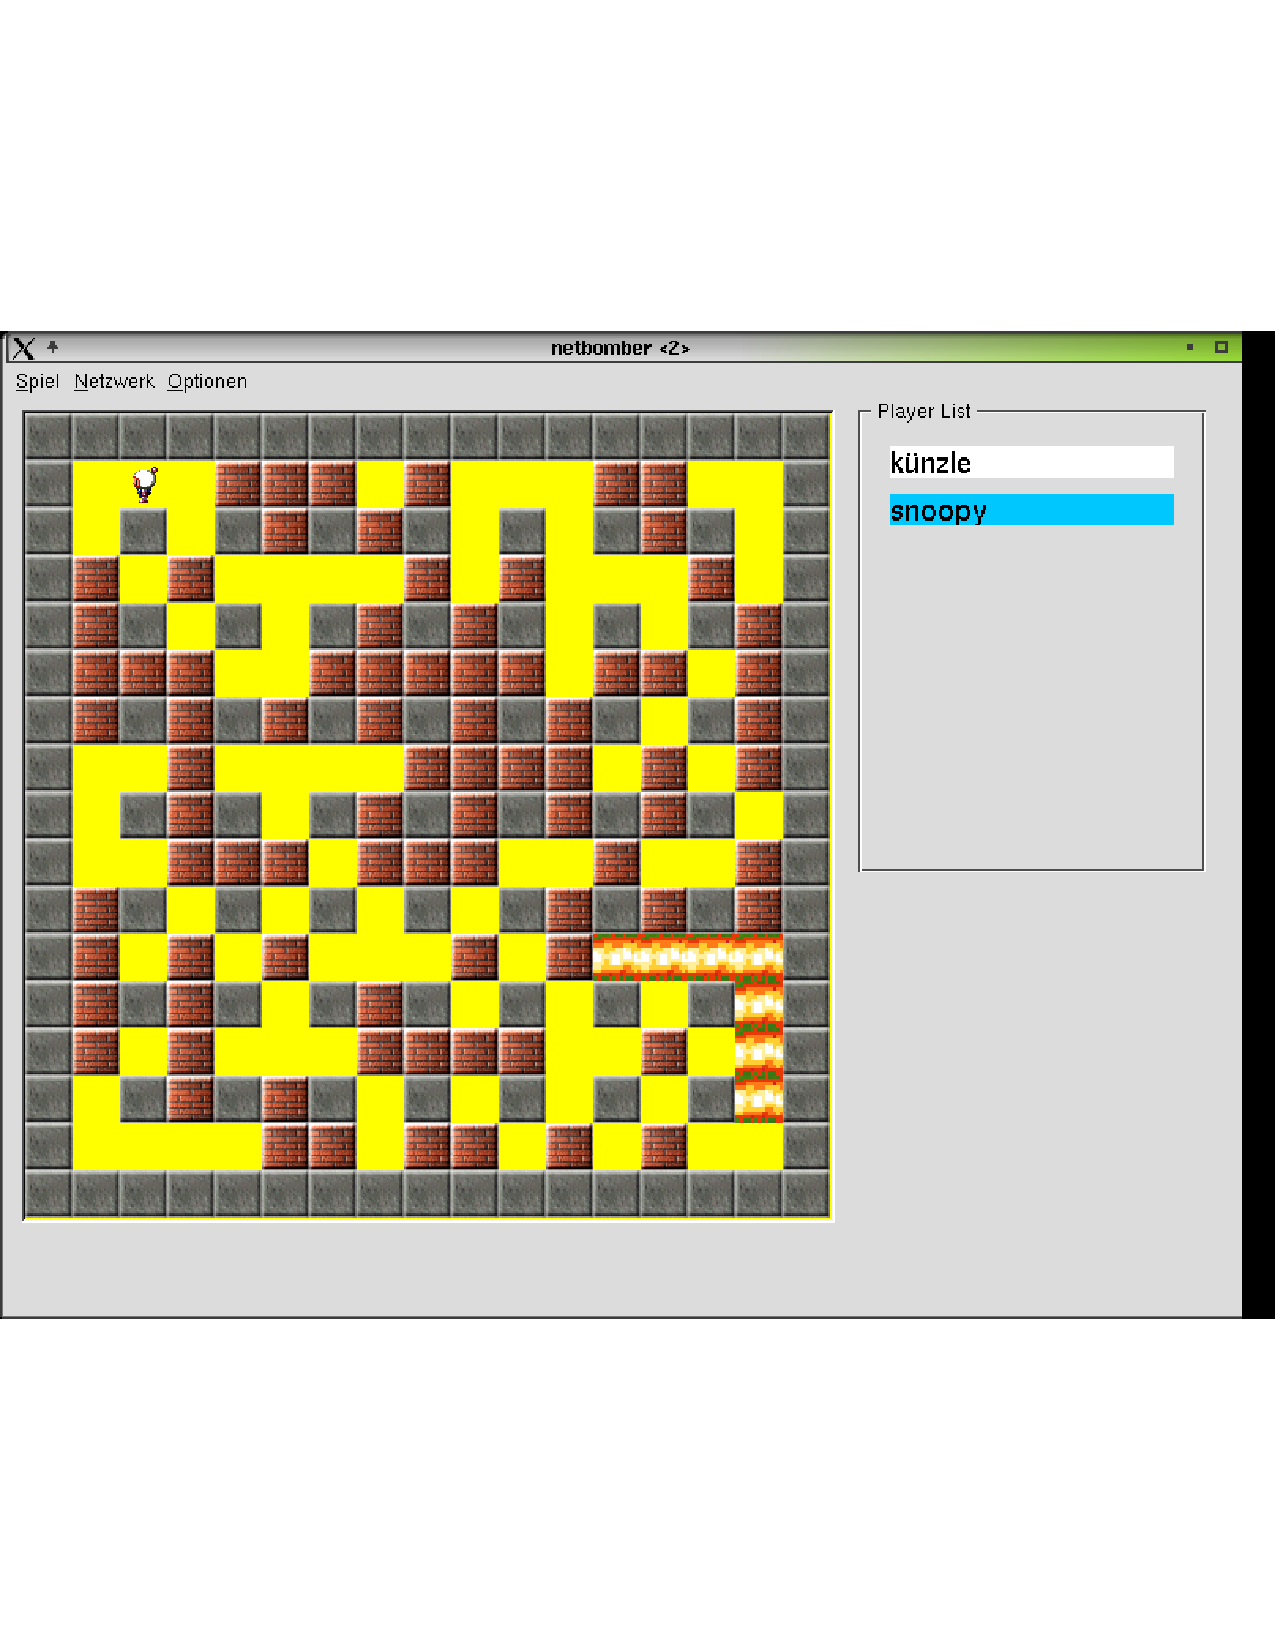
\includegraphics[width=10cm]{./images/spielfeld.pdf} \\
  \end{center}
  \caption{Bomberman Spiel}
\end{figure}

\subsection{Benutzergruppen}
Alle Menschen ob jung oder alt, weiblich oder m"annlich, die Freude an Computerspielen haben.

\subsection{M"ogliche Erweiterungen}
\begin{itemize}
\item Sound Unterst"utzung
\item spezielle Powerup-Icons, die von der Spielfigur aufgenommen werden k"onnen.
\item Highscore Anzeige
\end{itemize}

\subsection{Zu erwartende Probleme}
wurden bereits im Dokument Projektplan eingetragen.

\subsection{Annahmen}
Da die von uns verwendeten Technologien f"ur uns neu sind, sind wir uns bewusst, dass das Risiko vorhanden ist, dass wir
die Anforderungen nicht vollst"andig erf"ullen k"onnen. Dieses Dokument wurde in der Annahme geschrieben, dass wir die
auftretenden Probleme l"osen k"onnen. Ansonsten werden wir die Anforderungen zusammen mit dem Betreuer anpassen.

\subsection{Abh"angikeiten}
Funktionalit"at Qt-Bibliothek und KDE-Bibliothek.

\section{Anforderungen im Einzelnen}

\subsection{Funktionale Anforderungen Iteration 1}


\begin{table}[H]
  \begin{center}
    \begin{tabular}{|p{20mm}| p{85mm}| p{20mm}|}
    \multicolumn{3}{l}{\textbf{Spiel}} \\
    \hline Referenz & Funktion & Priorit"at \\
    \hline A1.1 & Spiel starten & 1 \\
    \hline A1.2 & Spiel beenden & 1 \\
    \hline A1.3 & Spielregeln "uberwachen & 1 \\
    \hline
    \end{tabular}
  \end{center}
  \caption{Spiel Funktionen Iteration 1}
\end{table}

\begin{table}[H]
  \begin{center}
    \begin{tabular}{|p{20mm}|p{85mm}|p{20mm}|}
    \multicolumn{3}{l}{\textbf{Spielfigur}} \\
    \hline Referenz & Funktion & Priorit"at \\
    \hline A2.1 & Figur bewegen & 1 \\
    \hline
    \end{tabular}
  \end{center}
  \caption{Spielfigur Funktionen Iteration 1}
\end{table}


\begin{table}[H]
  \begin{center}
    \begin{tabular}{|p{20mm}|p{85mm}|p{20mm}|}
    \multicolumn{3}{l}{\textbf{Spielfeld}} \\
    \hline Referenz & Funktion & Priorit"at \\
    \hline A3.1 & Hintergrund zeichnen & 1 \\
    \hline A3.2 & Mauern und W"ande zeichnen & 1 \\
    \hline A3.3 & Spielfigur zeichnen & 1 \\
    \hline
    \end{tabular}
  \end{center}
  \caption{Spielfeld Funktionen Iteration 1}
\end{table}


\subsection{Funktionale Anforderungen Ieration 2}


\begin{table}[H]
  \begin{center}
    \begin{tabular}{|p{20mm}|p{85mm}|p{20mm}|}
    \multicolumn{3}{l}{\textbf{Spiel}} \\
    \hline Referenz & Funktion & Priorit"at \\
    \hline A1.4 & Spielstand aktualisieren & 2 \\
    \hline A1.5 & Highscore speichern & 2 \\
    \hline
    \end{tabular}
  \end{center}
  \caption{Funktionen Spiel Iteration 2}
\end{table}



\begin{table}[H]
  \begin{center}
    \begin{tabular}{|p{20mm}|p{85mm}|p{20mm}|}
    \multicolumn{3}{l}{\textbf{Spielfigur}} \\
    \hline Referenz & Funktion & Priorit"at \\
    \hline A2.2 & Bombe legen  & 2 \\
    \hline A2.3 & sterben      & 2 \\
    \hline
    \end{tabular}
  \end{center}
  \caption{Funktionen Spielfigur Iteration 2}
\end{table}



\begin{table}[H]
  \begin{center}
    \begin{tabular}{|p{20mm}|p{85mm}|p{20mm}|}
    \multicolumn{3}{l}{\textbf{Spielfeld}} \\
    \hline Referenz & Funktion & Priorit"at \\
    \hline A3.4 & Wand entfernen & 2 \\
    \hline
    \end{tabular}
  \end{center}
  \caption{Funktionen Spielfeld Iteration 2}
\end{table}



\begin{table}[H]
  \begin{center}
    \begin{tabular}{|p{20mm}|p{85mm}|p{20mm}|}
    \multicolumn{3}{l}{\textbf{Bombe}} \\
    \hline Referenz & Funktion & Priorit"at \\
    \hline A4.1 & explodieren & 2 \\
    \hline A4.2 & Reichweite berechnen & 2 \\
    \hline
    \end{tabular}
  \end{center}
  \caption{Funktionen Bombe Iteration 2}
\end{table}



\begin{table}[H]
  \begin{center}
    \begin{tabular}{|p{20mm}|p{85mm}|p{20mm}|}
    \multicolumn{3}{l}{\textbf{Netzwerk}} \\
    \hline Referenz & Funktion & Priorit"at \\
    \hline A5.1 & Server starten & 2 \\
    \hline A5.2 & Client anmelden & 2 \\
    \hline A5.3 & Spielelement Position "ubermitteln & 2 \\
    \hline A5.4 & Spielsituation synchronisieren & 2 \\
    \hline
    \end{tabular}
  \end{center}
  \caption{Funktionen Netzwerk Iteration 2}
\end{table}

%Use Cases
\subsection{Use Cases Iteration 1}
\subsubsection{UC01 Spiel starten}

\begin{table}[H]
  \begin{center}
    \begin{tabular}{|p{40mm}|p{90mm}|}
    \hline Ausl"osender Aktor & Spieler  \\
    \hline Zweck / Ziel & Spielfeld und Spielelemente zeichnen, Netzwerkverbindung aufbauen  \\
    \hline Priorit"at & 1 \\
    \hline Style & casual \\
    \hline Anforderungen &  Iteration 1: A1.1, A1.2, A3.1, A3.2, A3.3 \\
		                     &  Iteration 2: inkl.A5.1, A5.2, A5.3, A5.4\\
    \hline Vorbedingung & - \\
    \hline Nachbedingung & Spielfeld und Spielelemente gezeichnet, Netzwerkverbindung aufgebaut. \\
    \hline Bemerkungen & - \\
    \hline
    \end{tabular}
  \end{center}
  \caption{UC01 Spiel starten}
\end{table}


\begin{center}
  \begin{tabular}{p{65mm} p{65mm}}
  \multicolumn{2}{l}{\textbf{Grundlegender Ablauf}} \\
  & \\
  \textbf{Aktor} & \textbf{System} \\
  1. Benutzer startet neues Spiel &  \\
  &  2. Leveldaten einlesen  \\
  &  3. Spielfeld zeichnen \\
  &  4. Spielelemente zeichnen \\
  &  5. wartet auf Benutzereingabe\\
  \multicolumn{2}{l}{\textbf{Erweiterungen}} \\
  \(\ast\)a zu jeder Zeit kann der Spieler das Spiel beenden & \\
  \end{tabular}
\end{center}


\subsubsection{UC02 Spielfigur bewegen}

\begin{table}[H]
  \begin{center}
    \begin{tabular}{|p{40mm}|p{90mm}|}
    \hline Ausl"osender Aktor & Spieler \\
    \hline Zweck / Ziel & Aktor kann Spielfigur in horizontaler oder vertikaler Richtung bewegen \\
    \hline Priorit"at & 1\\
    \hline Style & casual \\
    \hline Zu erf"ullende Anforderungen & A1.3, A2.1, A3.3 \\
    \hline Vorbedingungen & UC01 \\
    \hline Nachbedingungen & Die Spielfigur wurde um ein Feld verschoben.\\
    \hline Bemerkungen & Dieser UC kann 1 oder n mal ausgef"uhrt werden. \\
    \hline
    \end{tabular}
  \end{center}
  \caption{UC02 Spielfigur bewegen}
\end{table}


\begin{center}
  \begin{tabular}{p{65mm} p{65mm}}
  \multicolumn{2}{l}{\textbf{Grundlegender Ablauf}} \\
  & \\
  \textbf{Aktor} & \textbf{System} \\
  1. Der Aktor verschiebt die Spielfigur um ein Feld nach links, rechts, oben oder unten. & \\
  & 2. zeichnet die Figur auf dem neuen Feld, sofern das Zielfeld nicht einer Wand oder einer Mauer enstpricht. \\
  \end{tabular}
\end{center}

\subsection{Use Cases Iteration 2}
\subsubsection{UC03 Bombe legen}

\begin{table}[H]
  \begin{center}
    \begin{tabular}{|p{40mm}|p{90mm}|}
    \hline Ausl"osender Aktor & Spieler  \\
    \hline Zweck / Ziel & Der Spieler legt eine Bombe, die nach einer gewissen Zeit explodiert und
		                      alle vernichtbaren Objekte, die sich in Reichweite befinden zerst"ort\\
    \hline Priorit"at & 2 \\
    \hline Style & casual \\
    \hline Anforderungen &  A1.1, A1.3, A2.1, A2.2, A2.3, A3.1, A3.2, A3.3, A3.4, A4.1, A4.2\\
    \hline Vorbedingung & UC01 \\
    \hline Nachbedingung & Objekte die sich innerhalb der Reichweite befunden haben sind zerst"ort. \\
    \hline Bemerkungen & - \\
    \hline
    \end{tabular}
  \end{center}
  \caption{UC03 Bombe legen}
\end{table}


\begin{center}
  \begin{tabular}{p{65mm} p{65mm}}
  \multicolumn{2}{l}{\textbf{Grundlegender Ablauf}} \\
  & \\
  \textbf{Aktor} & \textbf{System} \\
  1. Der Spieler legt eine Bombe &  \\
	2. Der Spieler bewegt sich auf ein anderes Feld& \\
  &  3. Auf dem alten Feld wird eine Bombe dargestellt  \\
  &  4. Ein Timer startet \\
  &  5. Der Timer ist abgelaufen, auf allen Feldern (horizontal und vertikal zur Bombe) in Reichweite 
	wird eine Explosion dargestellt \\
  &  6. Zerst"orbare Elemente, die sich auf diesen Feldern befunden haben werden zerst"ort\\
  \multicolumn{2}{l}{\textbf{Erweiterungen}} \\
  \(\ast\)a zu jeder Zeit kann sich der Spieler auf benachbarte, begehbare Felder bewegen & \\
  \end{tabular}
\end{center}



\subsection{Optional}


\begin{table}[H]
  \begin{center}
    \begin{tabular}{|p{20mm}|p{85mm}|p{20mm}|}
    \multicolumn{3}{l}{\textbf{Spiel}} \\
    \hline Referenz & Funktion & Priorit"at \\
    \hline A1.6 & Spiel pausieren & 3 \\
    \hline A1.7 & Soundeffekte abspielen & 3 \\
    \hline A1.8 & Musik abspielen & 3 \\
    \hline
    \end{tabular}
  \end{center}
  \caption{optionale Funktionen Spiel}
\end{table}



\begin{table}[H]
  \begin{center}
    \begin{tabular}{|p{20mm}|p{85mm}|p{20mm}|}
    \multicolumn{3}{l}{\textbf{Spielfigur}} \\
    \hline Referenz & Funktion & Priorit"at \\
    \hline A2.4 & Bombe-Powerup aufnehmen & 3 \\
    \hline A2.5 & Flamme-Powerup aufnehmen & 3 \\
    \hline
    \end{tabular}
  \end{center}
  \caption{optionale Funktionen Spielfigur}
\end{table}


\begin{table}[H]
  \begin{center}
    \begin{tabular}{|p{20mm}|p{85mm}|p{20mm}|}
    \multicolumn{3}{l}{\textbf{Spieloptionen}} \\
    \hline Referenz & Funktion & Priorit"at \\
    \hline A6.1 & Sound ein/aus & 3 \\
    \hline A6.2 & Highscores anzeigen & 3 \\
    \hline A6.3 & Spielername eingeben & 3 \\
    \hline
    \end{tabular}
  \end{center}
  \caption{Spieloptionen}
\end{table}


\subsection{Leistungs- und Mengenanforderungen}
\label{LeistungsAnforderungen2}
\subsubsection{Leistungsanforderungen}
Um die Spielbarkeit "ubers Netzwerk zu gew"ahrleisten, muss der Spielstatus von allen Spielern mindestens
alle 150ms synchronisiert werden.

\subsubsection{Mengenanforderungen}
Keine.

\subsection{Anforderungen an Schnittstellen}

\subsubsection{Benutzerschnittstelle}
Das System ist mit dem Keyboard und der Maus bedienbar.

\subsubsection{Software Schnittstellen}
Qt, KDE-Library

\subsection{Randbedingungen f"ur den Entwurf}

\subsubsection{"Ubereinstimmungen mit Normen}
SE01/02

\subsubsection{Einschr"ankungen bez"uglich Software}
Lauff"ahig unter KDE 2.2 mit Qt 2.3.1

\subsubsection{Einschr"ankungen bez"uglich Hardware}
Lauff"ahig unter allen UNIX-Derivaten, die KDE unterst"utzen. Die Leistungsanforderungen gelten f"ur ein Netzwerk (mind. 10Mb/s)
ohne zus"atzlichen Datenverkehr.

\subsection{Merkmale}

\subsubsection{Benutzbarkeit}
Die Bedienung des Programms entspricht den g"angigen KDE-Programmen:\\
\href{http://developer.kde.org/documentation/standards/kde/style/basics/index.html}{http://developer.kde.org/documentation/standards/kde/style/basics/index.html}

\subsection{Andere Anforderungen}

\subsubsection{Inbetriebnahme / Installation}
Standardinstallationsweg eines Linux-Quellcodes (configure, make, make install)
In der Datei README finden Sie bez"uglich Inbetriebnahme detaillierte Informationen.

\subsubsection{Konfigurierbarkeit}
Alle Konfigurationen werden gespeichert. Die IP-Adresse des Spielservers kann eingegeben werden.
Optional kann der Spielername eingegeben werden.






\chapter{Supplementary Specification}

\section{Functionality}

\subsection{Error handling}
Fehler werden dem Spieler mittels einer Fehlermeldung gemeldet.
Die Fehler werden nicht persistent in einer log-datei gespeichert.

\subsection{Security}
Das Programm hat keine speziellen Sicherheitsvorkehrungen. Es kommuniziert "uber ein IP-Netz mit den Programmen der anderen Spieler.

\section{Performance}
Mit den unter \ref{LeistungsAnforderungen} auf Seite \pageref{LeistungsAnforderungen} angegebenen Leistungsanforderungen soll ein angenehmes Spielverhalten gew"ahrleistet werden.
\section{Supportability}

\section{Free open source components}
Als Linux-Software-Developers liegt es Nahe, OpenSource Technologien zu verwenden.
(siehe dazu Projektplan, Kapitel Technologien)

\section{Developer Guidelines}

\subsection{Code Guidelines}

\begin{itemize}
  \item Methodennamen beginnen mit Kleinbuchstaben
  \item Klassennamen beginnen mit Grossbuchstaben
  \item Variabeln beginnen mit Kleinbuchstaben
  \item Vor und nach Operations-Zeichen wird ein Abstand gemacht.
  \item Nach zusammengeh"origen Code-Bl"ocken eine leere Zeile einf"ugen.
  \item Bei Klassen die "offnende geschweifte Klammer rechts neben dem Klassennamen und die schliessende auf eine eigene Zeile.
        F"ur alle anderen F"alle die "offnende und schliessende geschweifte Klammer auf eine eigene Zeile.
  \item Code innerhalb geschweifter Klammern wird einger"uckt.
  \item Falls Tabulatoren verwendet werden, in der Entwicklungsumgebung definieren, dass daf"ur Leerzeichen eingef"ugt werden.
  \item Default-Einr"uckung: Zwei Leerzeichen
  \item jede Kommentarzeile mit zwei slashes (//) beginnen.
\end{itemize}

\subsection{GUI Guidelines}
Folgt sp"ater in einem speraten Dokument.

\chapter{Domainanalyse}

\section{Konzeptionelles Modell}

\begin{figure}[H]
  \begin{center}
    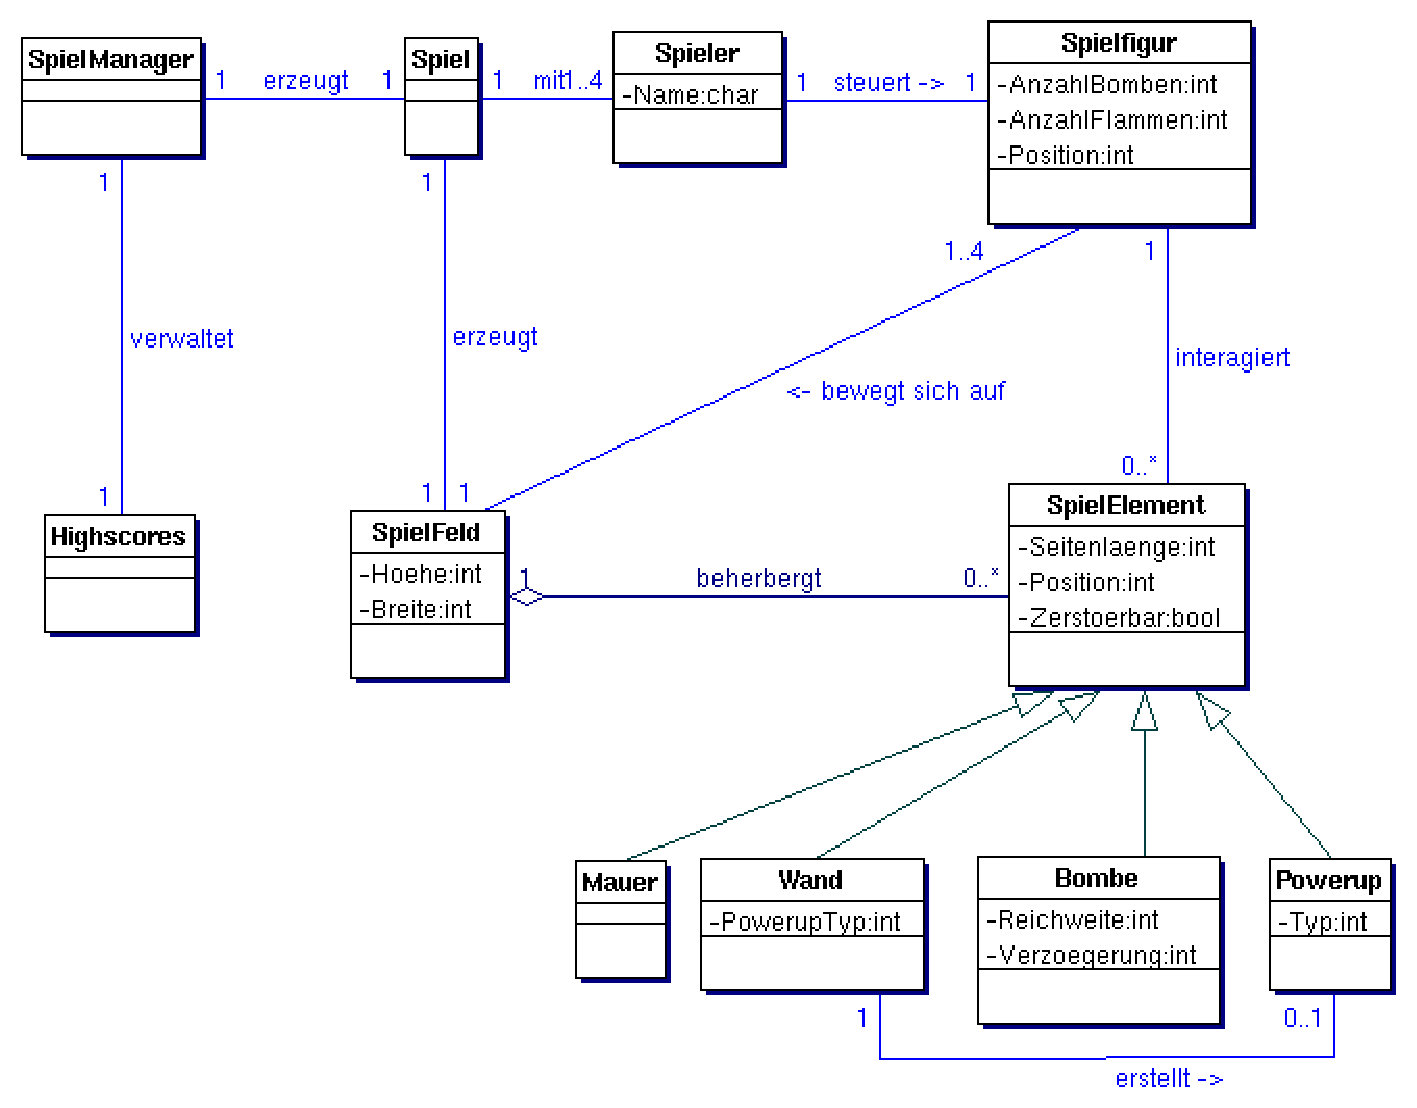
\includegraphics[width=14cm]{./images/domainmodell.pdf}
  \end{center}
  \caption{Domainmodell}
\end{figure}

\subsection{Spielmanager}
Der SpielManager ist f"ur die Initialisierung des Spiels zust�ndig. Er kennt die zwei Spieler und weitere f"ur das Spiel
notwendige Parameter.

\subsection{Spiel}
Das Spiel erzeugt das Spielfeld und positioniert die Spielelemente f"ur den Start des Spiels.

\subsection{Spielfeld}
Das Spielfeld ist der Hintergrund auf dem das eigentliche Spiel stattfindet. Es hat eine bestimmte H"ohe und Breite die zu beginn
festgelegt werden. Auf dem Spielfeld befinden sich die Objekte des Spielfeldes:Spielelemente und Spielfigur. Alle Objekte
des Spielfeldes haben eine Position. Das Spielfeld kennt alle Objekte und ihre Positionen.

\subsection{Spielelement}
Das Spielelement dient als Oberklasse f"ur s"amtliche sich auf dem Spielfeld befindlichen Objekte, ausser der Spielfigur.
Die einheitliche Schnittstelle erleichtert die Realisierung einiger Funktionen wie die Zerst"orung von Objekten usw.
Ein Objekt des Spielfeldes belegt normalerweise ein Feld auf dem Spielfeld.
Es kann "uber das Spielfeld die Belegung der benachbarten Felder abfragen.

\subsection{Spielfigur}
Die Spielfigur ist das einzige Objekt des Spielfeldes das sich auf dem Spielfeld bewegen kann. Sie kann mit den Spielelementen
kommunizieren. Die Spielfigur kann zum Beispiel Bomben erzeugen (legen) oder Powerups aufnehmen. Andererseits wird sie
von Mauern und W"anden am weitergehen gehindert.

\subsection{Mauer}
Die Mauer wird vor Spielbeginn erzeugt und bleibt w"ahrend dem ganzen Spiel an ihrem Platz. Sie kann nicht zerst"ort werden, trotzt
also auch explodierenden Bomben.

\subsection{Wand}
Die Wand wird ebenfalls zu beginn erzeugt, kann aber durch Bomben gesprengt werden und verschwindet in diesem Fall vom Spielfeld.
Eine Wand kann (muss aber nicht) ein Powerup beherbergen. Dieses bleibt auf dem Feld liegen falls die Wand zerst"ort wird.

\subsection{Bombe}
Die Bombe wird von der Spielfigur erzeugt. Dabei werden die Attribute wie Reichweite und Verz"ogerungszeit gesetzt. Danach ist
die Bombe ein eigenst"andiges Spielelement und explodiert entweder nach Ablauf der Verz"ogerungszeit oder wenn sie von einer
anderen Bombe gesprengt wird. Nach dem Explodieren meldet sie ihr Ableben der Spielfigur, die sie erzeugt hat.

\subsection{Powerup}
Ein Powerup ist entweder vom Typ Bombe (eine Bombe mehr in serie) oder vom Typ Flamme (gr"ossere Reichweit) und ist zu Beginn
unter einer Wand verborgen. Es tritt erst in erscheinung wenn die Wand durch eine Bombe zerst"ort wurde.
Betritt eine Spielfigur dasselbe Feld, nimmt sie das Powerup auf und es wird gel"oscht. Wird das Powerup von einer explodierenden
Bombe erfasst, wird es zerst"ort.

\subsection{Spieler}
Der Spieler hat einen Namen und steuert die Spielfigur. Er kann sie in alle 4 Richtungen bewegen und Bomben legen.

\chapter{Software Architektur}

\section{Logische Sicht}
Das System besteht aus prim"ar 4 Schichten (3  Schichten - Architektur plus Netzwerk). Diese beinhalten:
\begin{description}
\item[Schicht 1] Graphisches User Interface (GUI)
\item[Schicht 2] Problem Domain (PD)
\item[Schicht 3] Datenhaltung (DH)
\item[Schicht 4] Netzwerk (bestehend aus Client und Server)
\end{description}

\begin{figure}[H]
  \begin{center}
    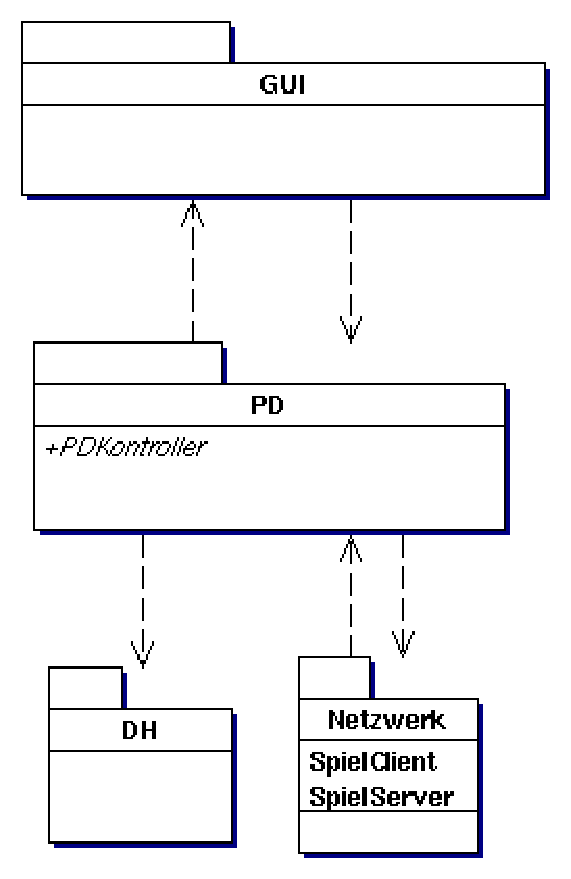
\includegraphics[height=8cm]{./images/architektur.pdf}
  \end{center}
  \caption{Schichtenmodell}
\end{figure}

Diese Architektur haben wir gew"ahlt um eine klare Trennung zwischen den einzelnen Programmteilen zu erreichen. \\
Das graphische User Interface ist die Schnittstelle zum Benutzer. "Uber dieses kann er Eingaben machen oder in unserem Fall erfolgt die Steuerung
der Spielfigur "uber das GUI. \\
Die PD ist die Schicht zwischen GUI und DH. Das heisst sie bekommt und verarbeitet Befehle vom GUI, schreibt Daten in die DH und
ruft Funktionen in der Netzwerkschicht auf. \\
Die Datenhaltung ist daf"ur zust"andig, Daten, die konsistent sein m"ussen zu speichern, damit sie bei einem Neustarten des Spiels wieder
zur Verf"ugung stehen. \\
Die Netzwerkschicht regelt die Daten"ubertragung zwischen dem Server und den Clients.



\section{Netzwerk}

\begin{figure}[hp]
  \begin{center}
    {\rotatebox{90}{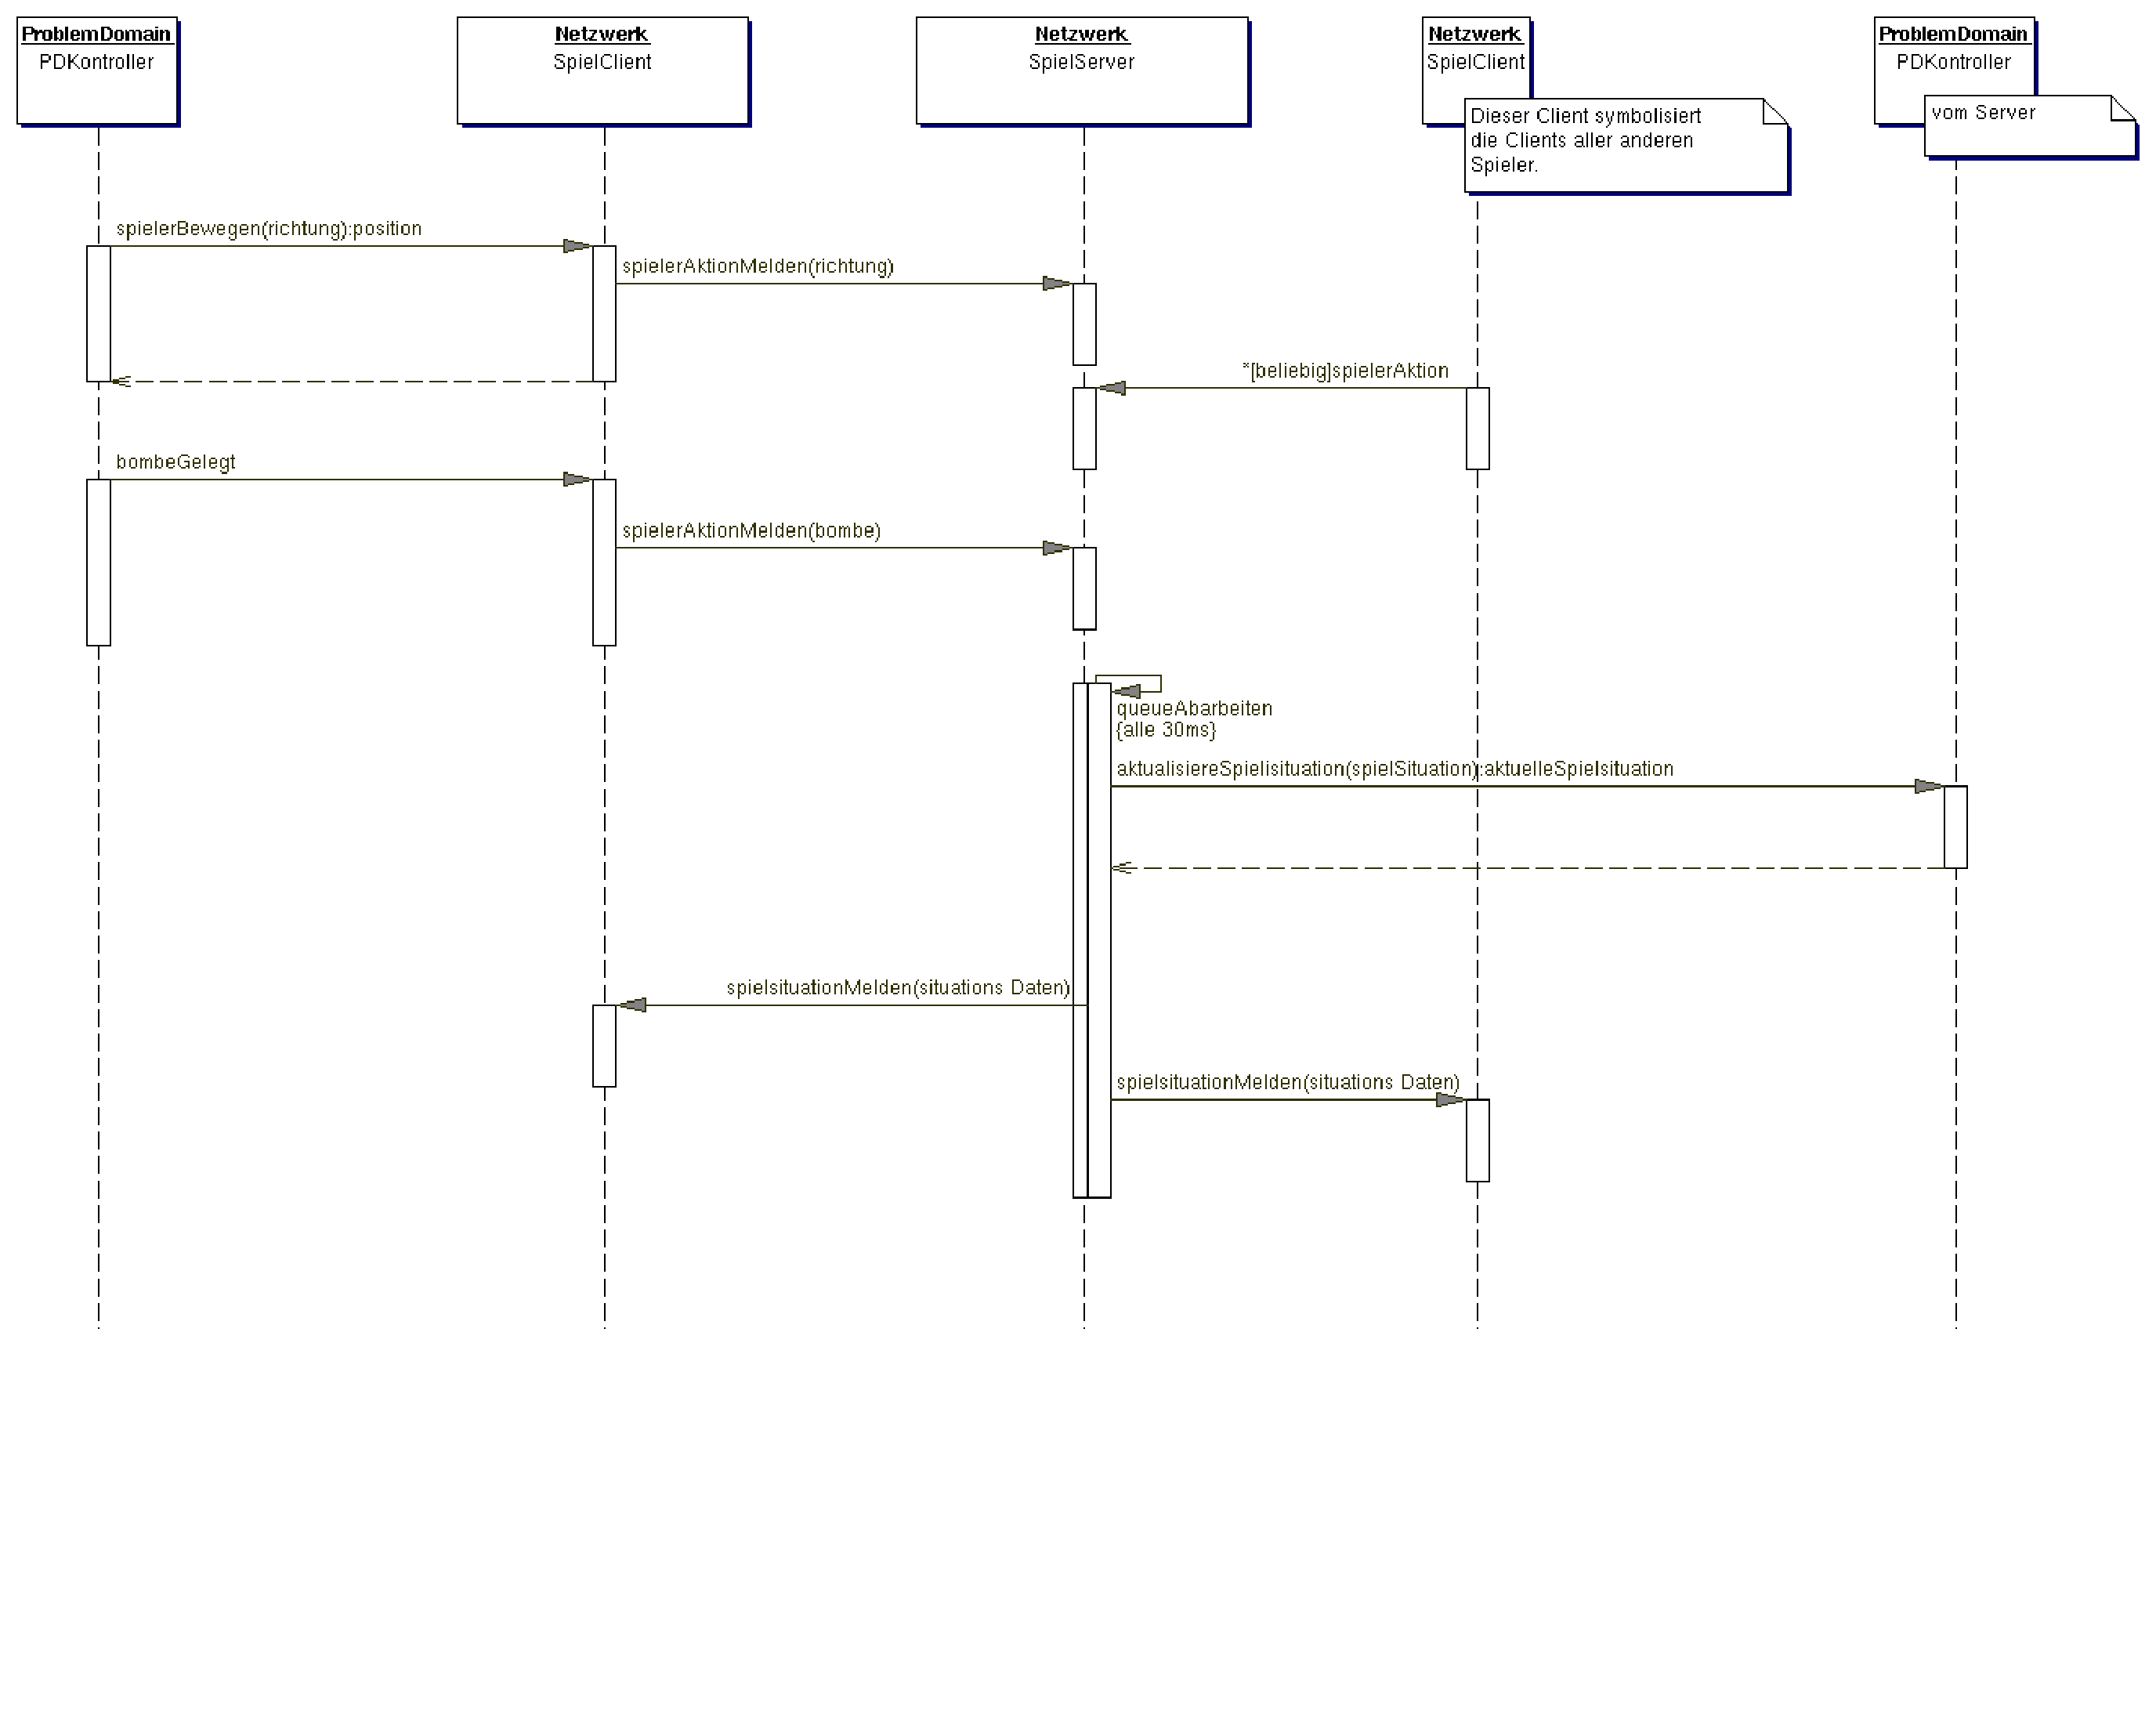
\includegraphics[height=16cm]{./images/netzwerk_aktion.pdf}}}
  \end{center}
  \caption{Interaktionsmodell Netzwerk}
\end{figure}

Das Netzwerk besteht aus einem Server und bis zu vier Clients die miteinander kommunizieren. Dabei kann jeder Client auch Server sein, das heisst
zu Beginn des Spiels entscheidet der Spieler, ob er Server und Client oder nur Client ist. Es kann nur ein Spieler Server sein.
Ist ein Spieler Server und Client, werden die Daten der Mitspieler zu ihm "ubermittelt. Das geschieht folgendermassen: \\
Die aktuellen Bewegungen eines Clients, also eines Spielers, werden zum Server "ubermittelt. Diese Daten werden vom Server
entgegengenommen. Dieser berechnet damit die aktuelle Position und allf"allige Aktionen des Clients. Diese berechnete Postion schickt der Server dann \textit{allen} Clients
zur"uck. Das heisst, jeder Client bekommt vom Server einen Snapshot. Zus"atzlich zur Position beinhaltet dieser wichtige Daten wie zum Beispiel ob
eine Bombe gelegt worden ist oder ein Powerup aufgenommen wurde. Mit diesen Angaben berechnet der Client selbst"andig, was auf dem
Spielfeld passiert. Er macht also dieselben Berechnungen wie der Server. Falls ein Spielelement gel"oscht werden muss,
versucht der Client das zu machen. Da er aber nicht selbst"andig Elemente l"oschen darf, wartet er auf den Befehl des Servers,
das entsprechende Element zu l"oschen. Der Client f"uhrt also nur eine Art Dummy-Funktion aus.
Damit erreichen wir eine bessere Performace wie mit dem Prinzip, bei dem alle Daten vom Server zum Client geschickt werden und zudem
k"onnen wir damit sicherstellen, dass alle Clients den selben Spielstand haben. Die Verbindung l"auft "uber TCP, was das Ankommen
der Pakete sicherstellt. \\
Der Server wurde mit dem Reactor Pattern implementiert. Dieses wird nachfolgend noch genauer erkl"art.

\chapter{Designmodell}

%begin pd design
\section{GUI Externes Design}

\begin{figure}[H]
  \begin{center}
    {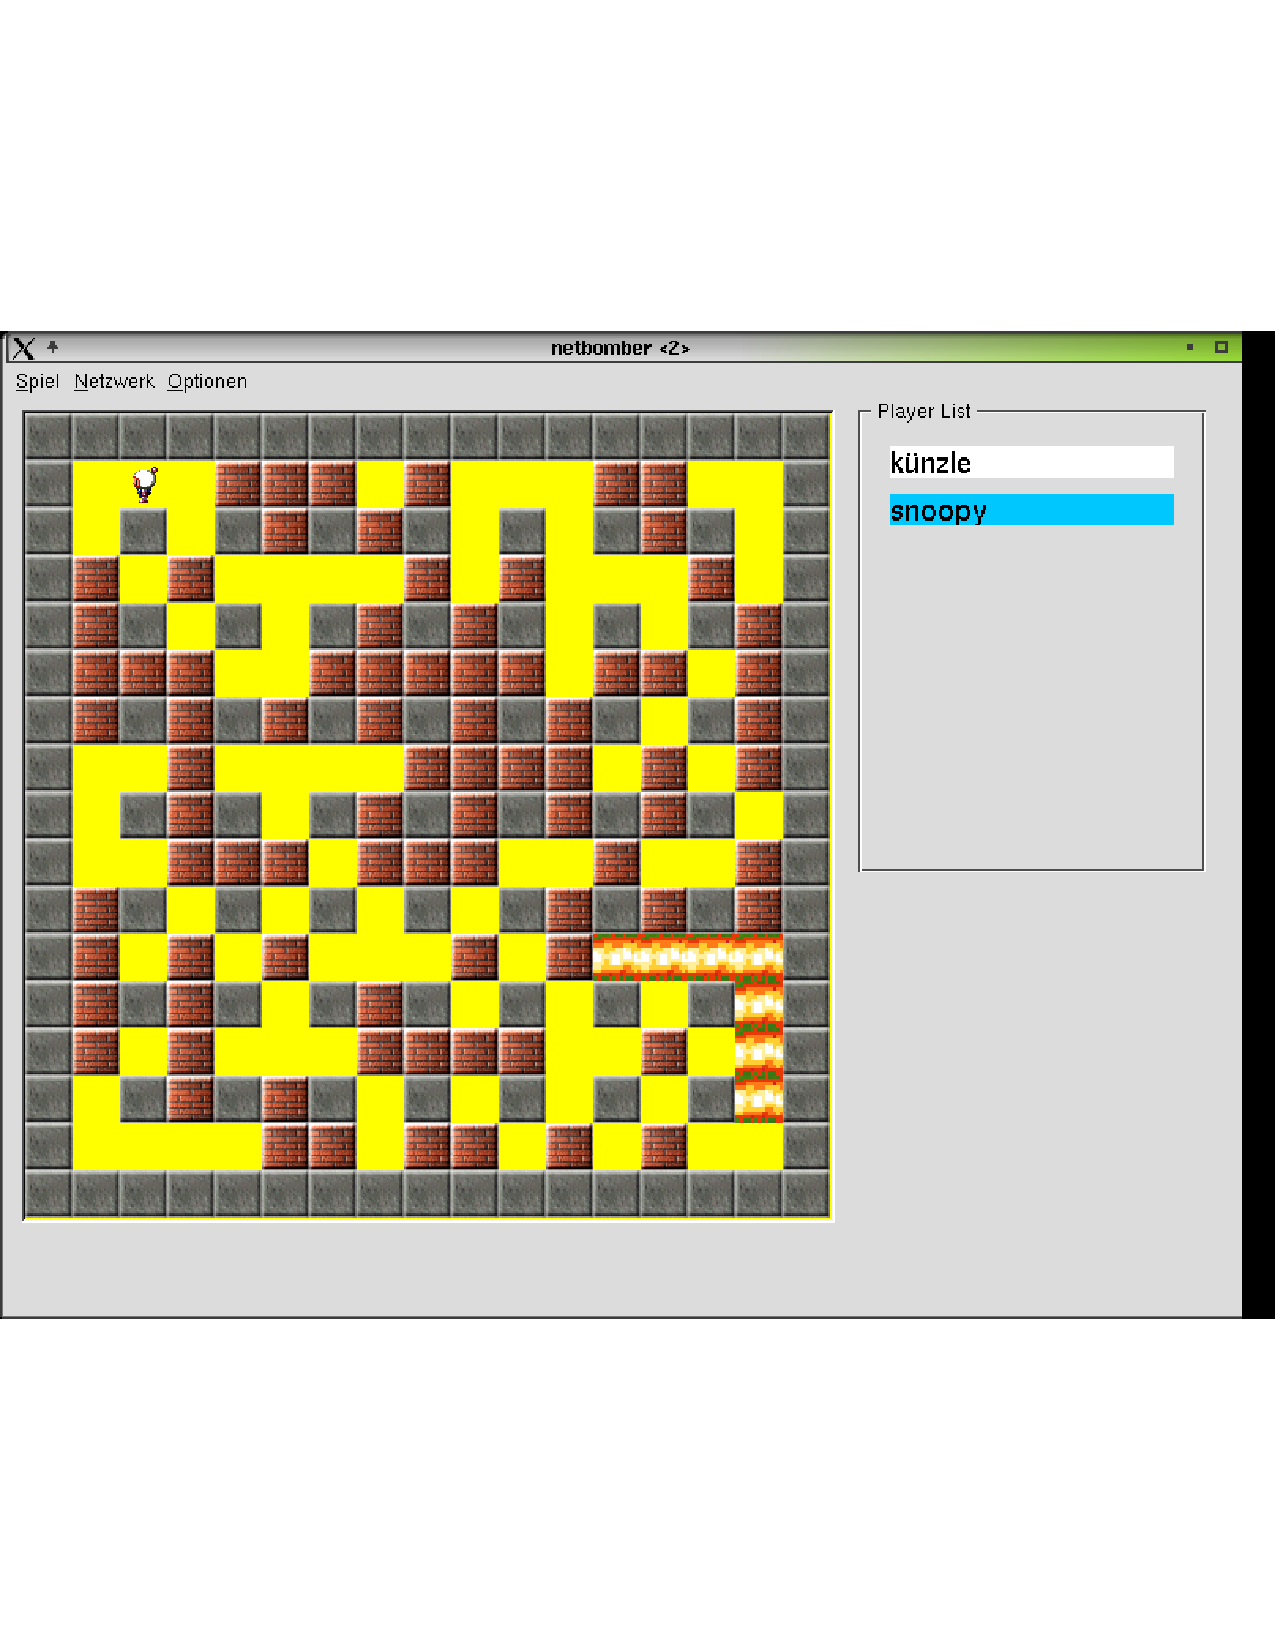
\includegraphics[height=12cm]{./images/spielfeld.pdf}}
  \end{center}
  \caption{Endversion des GUIs}
\end{figure}
Das Spielfeld (links) besteht aus diversen Spielelementen.
Diese werden dynamisch geladen, je nach dem was der Server
verlangt zum Darstellen. Rechts vom Spielfeld befindet sich
die Playerlist. Jeder Spielername wurde unterschiedlich
eingef"arbt, genau so wie die Farbe des entsprechenden Kopfes
der Spielfigur.

Die Farben der Spielfiguren:
\begin{table}[H]
	\begin{center}
		\begin{tabular}{|p{50mm}|p{30mm}|p{60mm}|}
		\hline Spielfigur 1 & Weiss & RGB (255, 255, 255) \\
		\hline Spielfigur 2 & Blau  & RGB (0, 200, 255) \\
		\hline Spielfigur 3 & Gr"un  & RGB (60, 255, 0) \\
		\hline Spielfigur 4 & Violet & RGB (255, 60, 255) \\
		\hline 
	\end{tabular}
	\end{center}
	\caption{Farben der Spielfiguren}
\end{table}


\begin{figure}[H]
  \begin{center}
    {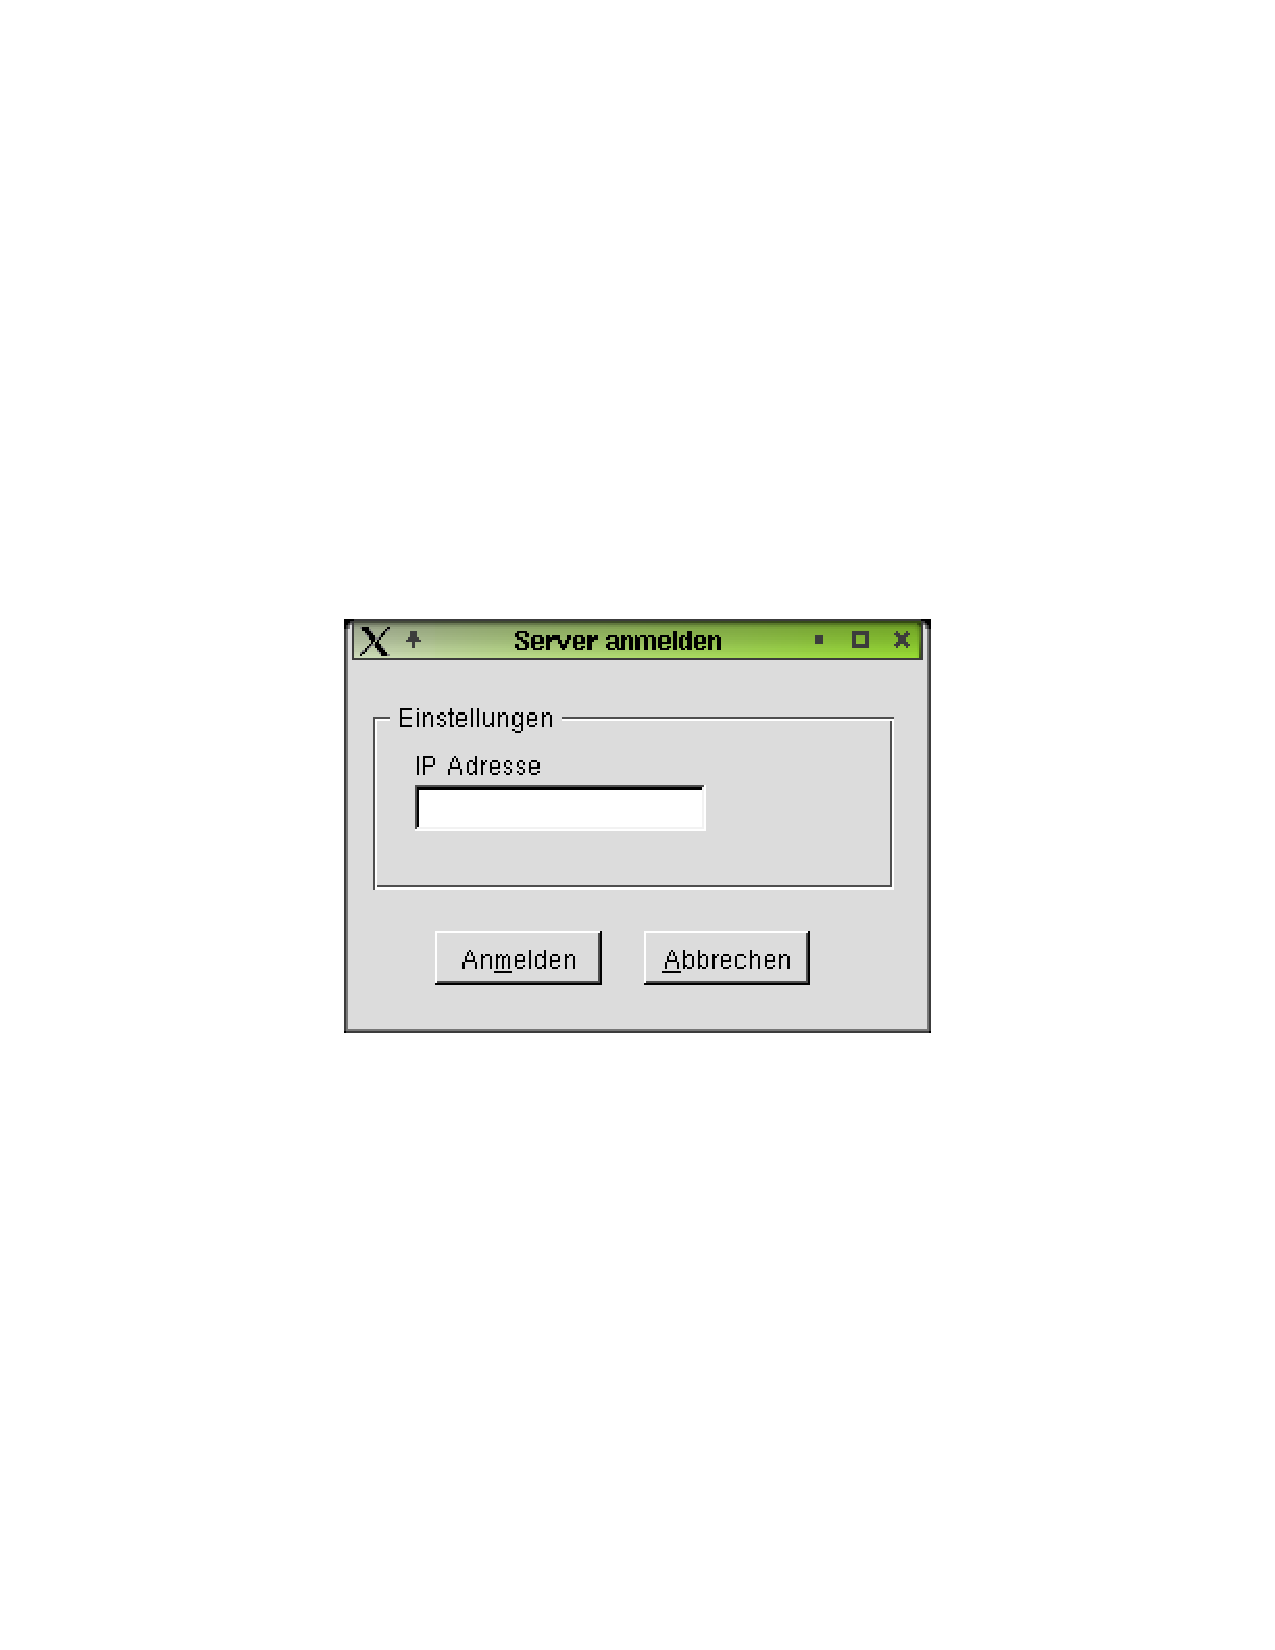
\includegraphics[height=6cm]{./images/joinserver.pdf}}
  \end{center}
  \caption{Snapshot des Dialoges Server anmelden}
\end{figure}

Dieser Dialog dient zum Anmelden an einen Server.

\begin{figure}[H]
  \begin{center}
    {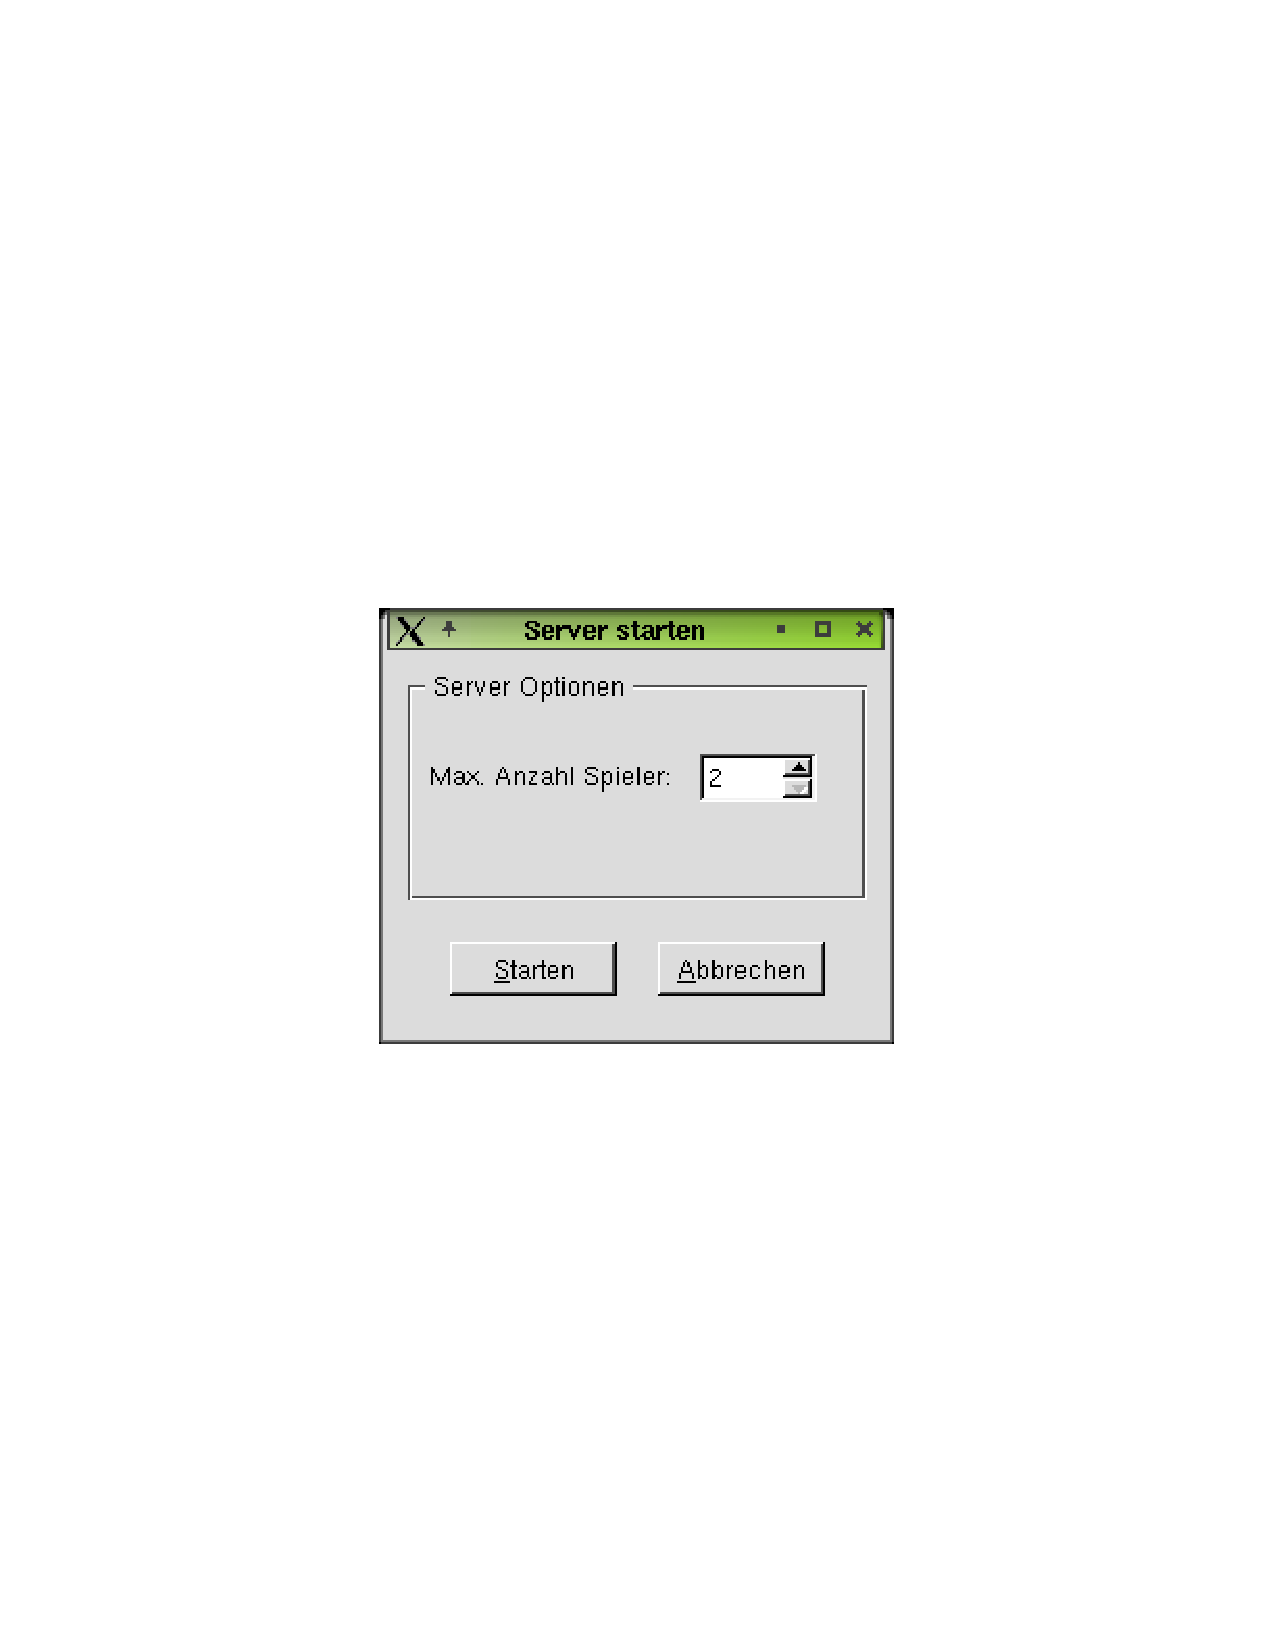
\includegraphics[height=6cm]{./images/startserver.pdf}}
  \end{center}
  \caption{Snapshot des Dialoges Server starten}
\end{figure}

Dieser Dialog dient zum Starten eines Servers.

\begin{figure}[H]
  \begin{center}
    {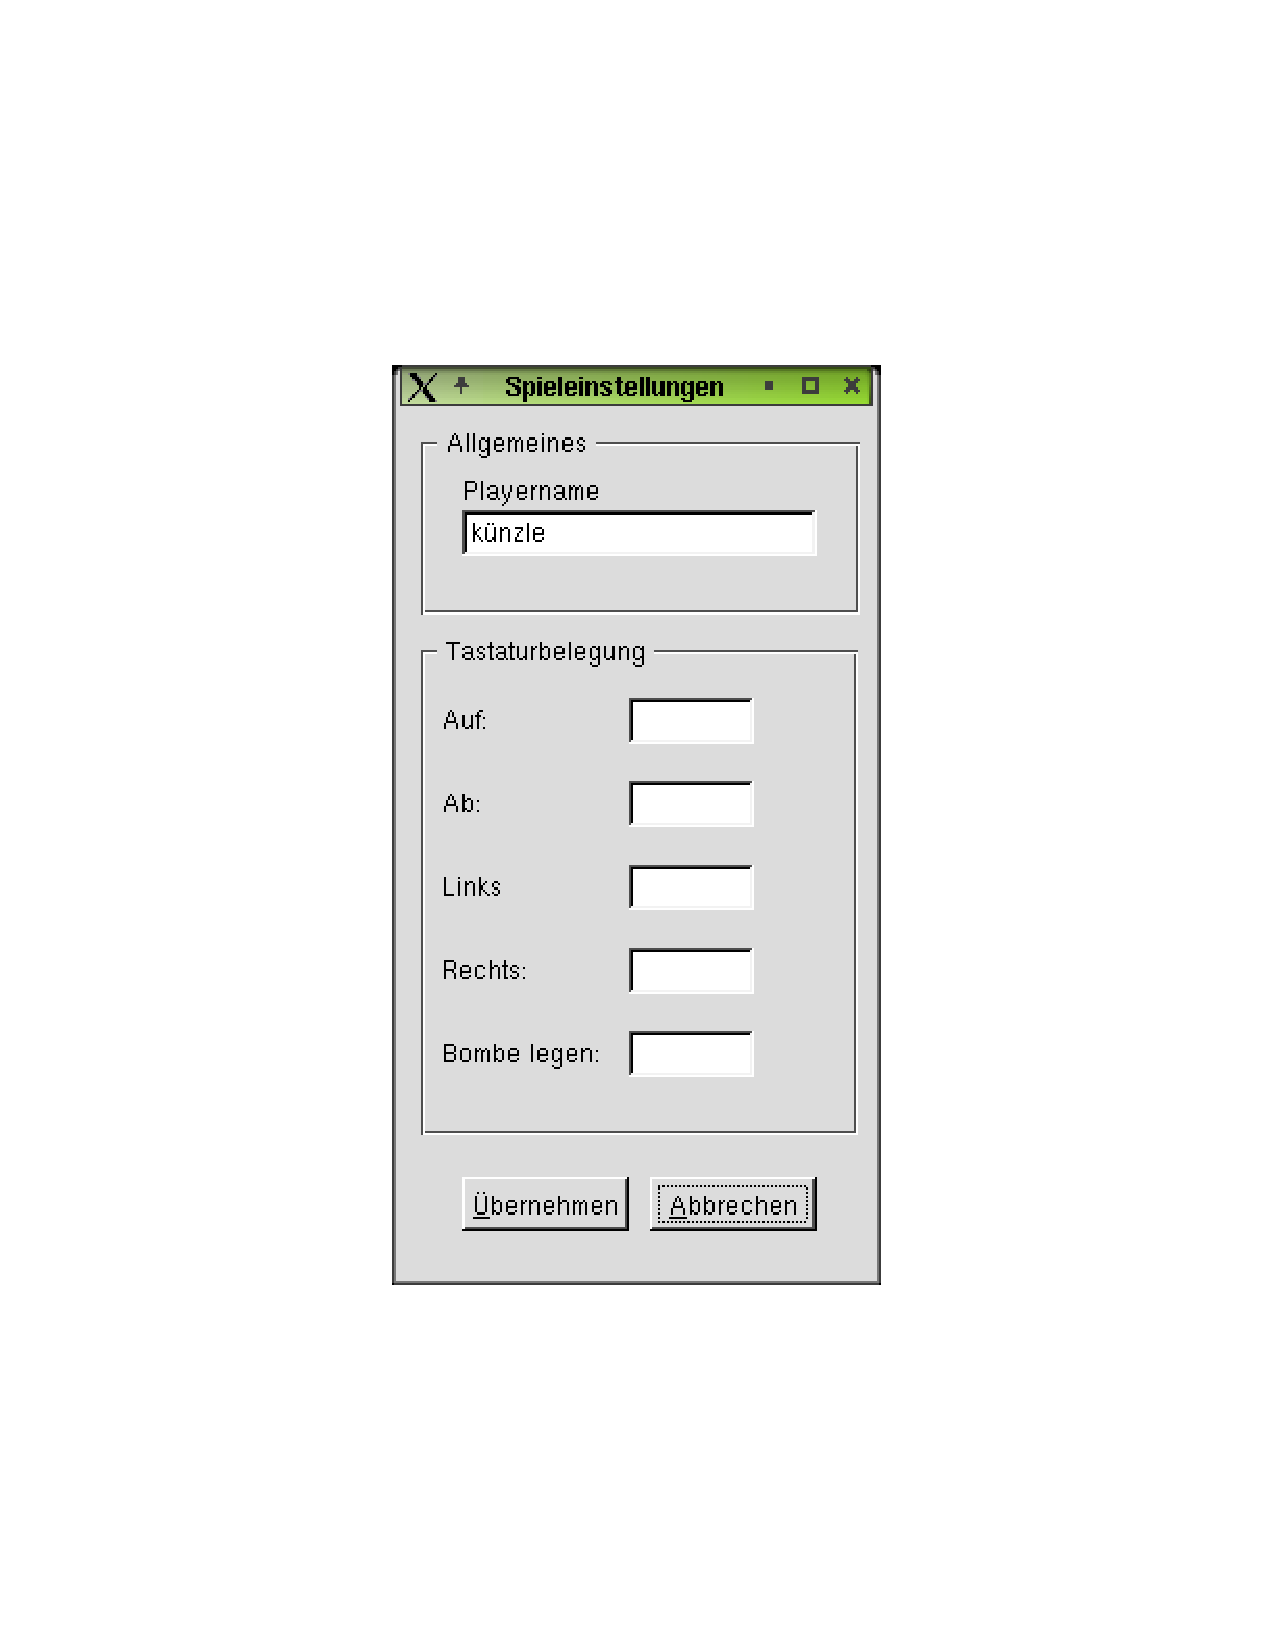
\includegraphics[height=10cm]{./images/settings.pdf}}
  \end{center}
  \caption{Snapshot des Dialoges Einstellungen}
\end{figure}

Dieser Dialog dient prim"ar zum Konfigurieren des Spielernamens.
Leider reichte uns die Zeit nicht mehr, die Tastaturbelegung
variierend zu machen. Vorgesehen war es jedoch in diesem Dialog.


\section{GUI Klassendiagramm}

Das gesamte Klassendiagramm befindet sich im Register Nr. 9.

\section{GUI Sequenzdiagramme}

\begin{figure}[H]
  \begin{center}
    {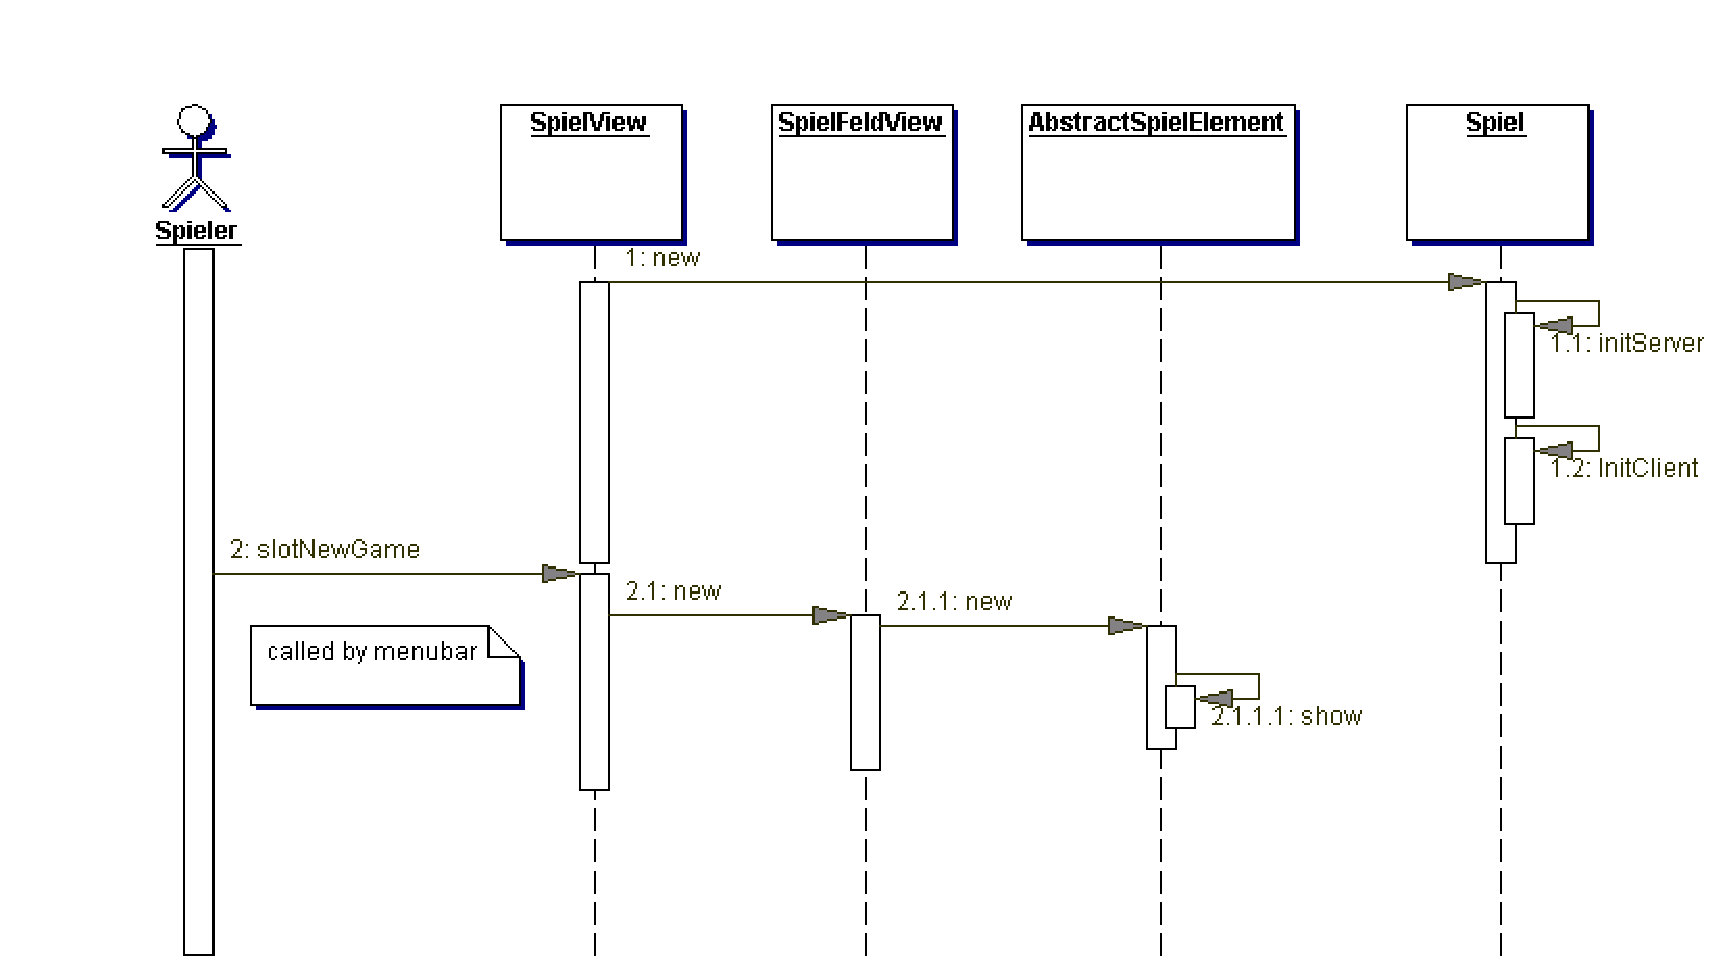
\includegraphics[height=6cm]{./images/neuesSpiel.pdf}}
  \end{center}
  \caption{Sequenzdiagramm f"ur neues Spiel}
\end{figure}



\begin{figure}[H]
  \begin{center}
    {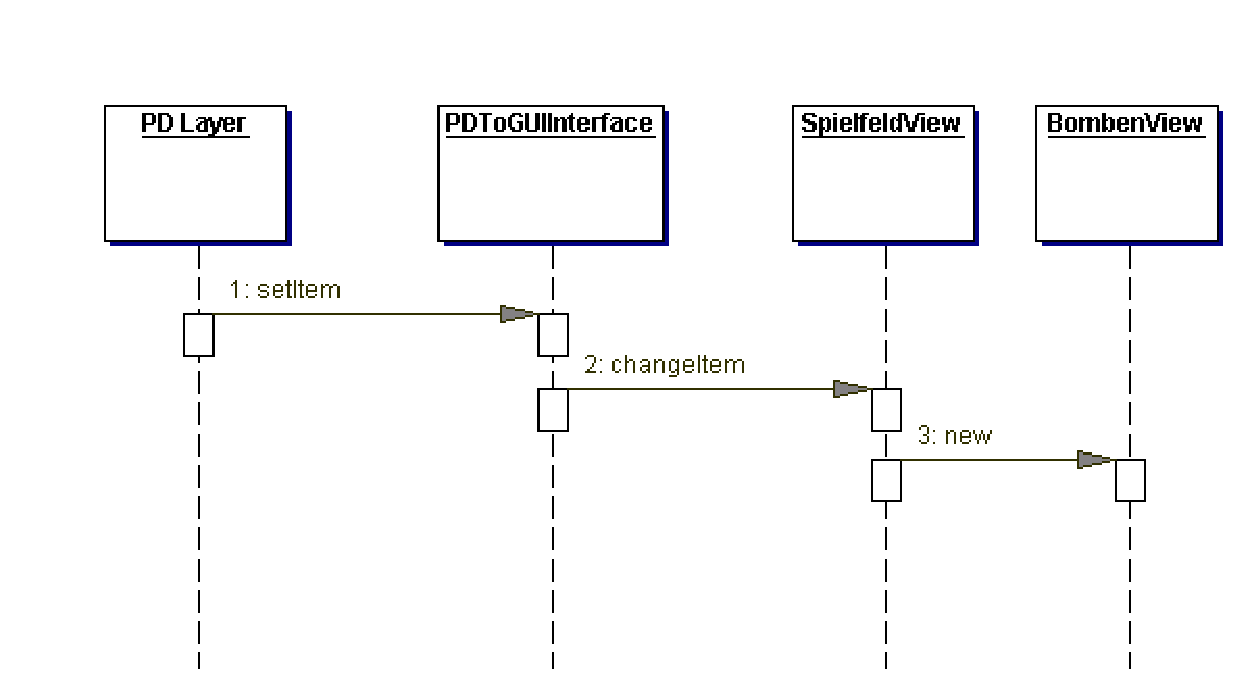
\includegraphics[height=6cm]{./images/bombeLegen.pdf}}
  \end{center}
  \caption{Sequenzdiagramm f"ur Bombe legen}
\end{figure}

Die PD wird hier als Blackbox betrachtet. Diese ruft "uber das
PDToGUIInterface setItem auf, wobei setItem als Parameter
den typ BOMBE und die Koordinaten x und y beinhaltet.
Die PDToGUIInterface Instanz teilt diese Anforderung der SpielfeldView
Instanz mit, welche dann mit dem Erzeugen einer neuen BombenView
Instanz reagiert.

\begin{figure}[H]
  \begin{center}
    {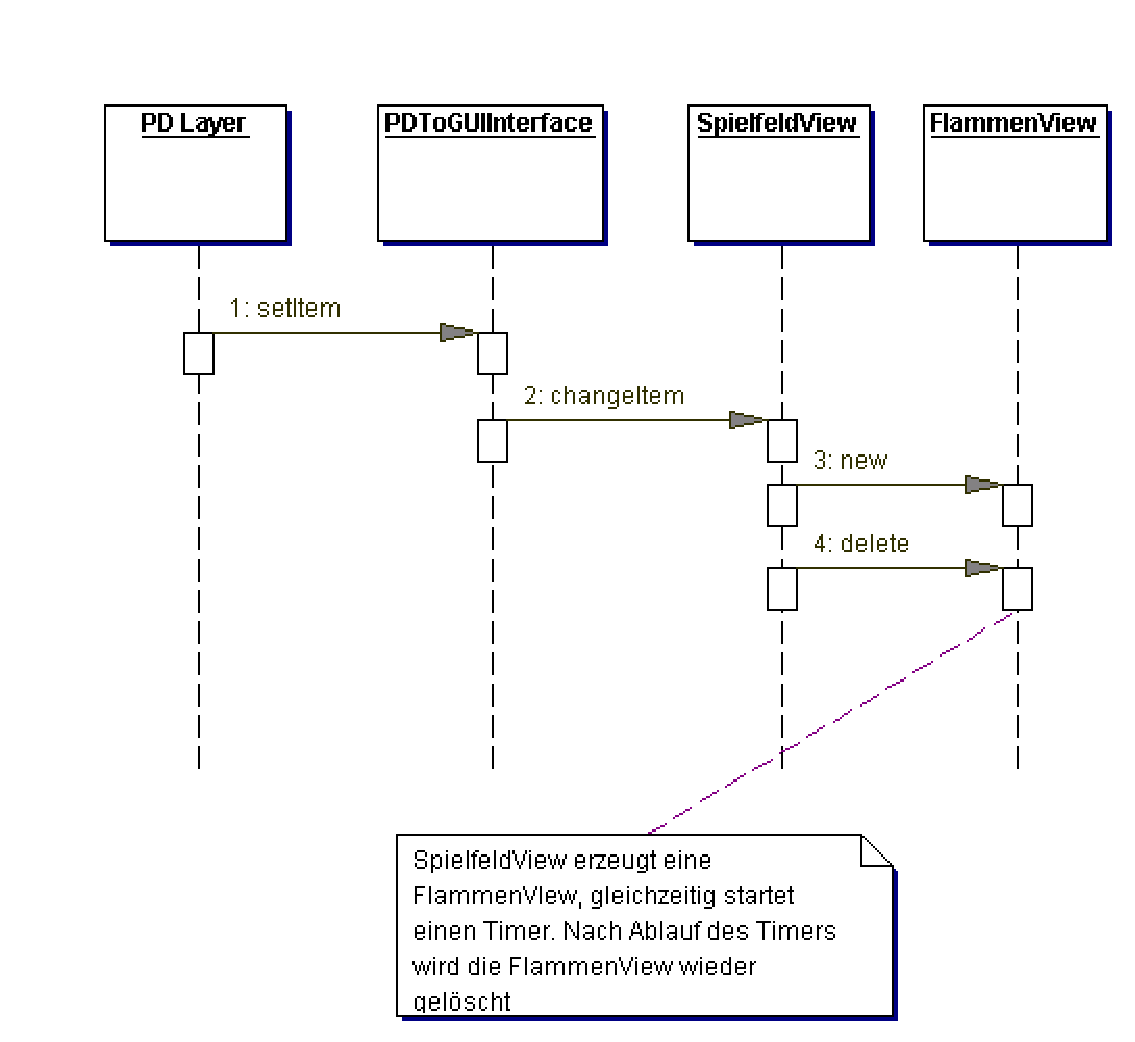
\includegraphics[height=6cm]{./images/neueflamme.pdf}}
  \end{center}
  \caption{Sequenzdiagramm f"ur eine Flamme anzeigen}
\end{figure}

Wieder vom PD Layer her kommt die Anforderung mit einem setItem.
Diesmal mit den Parametern FLAMME als typ und die Koordinaten x und y.
Die PDToGUIInterface Instanz leitet die Anforderung an die Instanz von SpielfeldView
weiter.
Die SpielfeldView Instanz erzeugt danach eine neue FlammenView Instanz. Gleichzeitig
startet einen Timer (QTimer), welcher nach Ablauf den Slot timerDone() aufruft.
In timerDone() wird die FlammenView wieder zerst"ort. Das bewirkt im Spiel selber
das kurze Erscheinen der Flamme, sozusagen explosionsartig.


\section{GUI Klassenbeschreibung}

\subsection{Klasse SpielView}

Die Klasse SpielView enth"alt einzig allein ein Menu. "Uber dieses kann der Spieler
einen Server starten, sich bei einem Server anmelden, Einstellungen vornehmen
und last but not least das Spiel starten bezw. beenden.
Um dies zu erm"oglichen, hat die Klasse SpielView Pointers auf die Klassen
JoinServerView, ServerView und SpielOptView. Diese werden bei den entsprechenden
Slots (Callbacks des Menus), mit show() aufgerufen.
Diese Klasse assoziiert ebenfalls mit der Klasse SpielFeldView, sozusagen
der Hauptklasse des GUIs (siehe unten). Im Konstruktur wird diese erzeugt, jedoch noch
nicht angezeigt. Dies erfolgt erst nachdem der Menupunkt Spiel starten ausgew"ahlt wurde.


\subsection{Klasse SpielFeldView}

Sie ist sozusagen die Kernklasse im GUI Design. Diese Klasse verwaltet alle
sich auf dem Spielfeld befindenen Elementen (Aggregation zu AbstractSpielElementView).
Um das zu erreichen, wird sie von der Klasse QCanvasView abgeleitet. QCanvasView
ist die Pr"asentationsklasse f"ur QCanvasItems, also f"ur einzelne Grafikelementen. Auch das
Keyboard-Eventhandling erfolgt in dieser Klasse. Falls Keyboard-Events auftreten,
werden diese abgefangen, und nur die f"ur das Spiel relevanten Steuersignale werden
der Klasse PDToGUIInterface weitergeleitet, wo sie dann von der PD verarbeitet werden.
Gleichzeitig erh"alt sie von der Klasse GUIToPDInterface Methodenaufrufe, welche das Ver"andern
des UI's zur Folge haben. Dies beinhaltet Items hinzuf"ugen und entfernen (Bombe und Flamme),
die Richtung der Spielfigur festlegen (um das entsprechende Sprite zu laden) und die Figur an
eine andere Koordinate bewegen. Um die Spielfigur eindeutig zu identifizieren, hat die Methode
moveXY() zus"atzlich den Paramter ID, dessen Wert die PD weiss.
Diese Klasse ist fast intelligenzlos. Sie nimmt nur Befehle von der Interfaceklasse entgegen,
oder leitet an diese Steuersignale weiter.

\subsection{Klasse SpielfigurView}

Diese Klasse repr"asentiert die Spielfigur. Sie wird im Konstruktor der Klasse SpielFeldView
erzeugt. Ihre Koordinaten erh"alt sie ebenfalls von der Klasse SpielFeldView.
Um grafisch ansprechende Animationen zu erm"oglichen, ist sie von der Klasse QCanvasSprite
abgeleitet. Diese Klasse erm"oglicht das dynamische Laden von Bildern (Frames), welche
durch entsprechende Methoden zu einer Animation zusammengesetzt werden k"onnen. In der Methode
advance(int step) erfolgt die eigentliche Animation in zwei Schritten: Wenn step 0 ist, hat
man die M"oglichkeit, die Items auf dem Spielfeld auf Kollision zu "uberpr"ufen (collision detection).
Im zweiten Schritt (step ist 1) werden die Items, in unserem Fall die Spielfigur, bewegt.
Diese Methode wird von Qt aufgerufen, vorausgesetzt das setAnimated(true) aiufgerufen wurde.

\subsection{Klasse AbstractSpielElementView}

Diese Klasse wurde von der Klasse QCanvasPolygonalItem abgeleitet. Sie erg"anzt diese
Klasse nur mit den Koordinaten. Gleichzeitig dient sie als Oberklasse f�r alle
auf dem Spielfeld befindenen Elementen, ausser der Spielfigur. Dies ist notwendig,
um die Aggregation zwischen SpielFeldView und AbstractSpielElement zu erreichen.

\subsection{Klasse MauerView}

Sie repr"asentiert auf dem Spielfeld eine unzerst"orbare Mauer. Das Attribut
rtti steht f"ur run time type information. Sie dient zur Identifikation.

\subsection{Klasse BombenView}

Sie repr"asentiert eine Bombe auf dem Spielfeld.

\subsection{Klasse FlammenView}

Sie repr"asentiert eine Flamme auf dem Spielfeld.

\subsection{Klasse ServerView}

Diese Klasse repr"asentiert einen Dialog, "uber welchen
einen Server gestartet werden kann. Als Option kann die
max. Anzahl Spieler festgelegt werden, nach dem Motto
""Server ist K"onig"".
Die Anmeldung erfolgt via den Klassen SpielView und GUIToPDInterface
zur PD mit dem Callback (Slot) bStartenPressed.

\subsection{Klasse JoinServerView}

Diese Klasse repr"asentiert einen Dialog, "uber welchen
sich ein Spieler an einen Server anmelden kann. Das einzige,
was der Spieler tun muss, ist eine g"ultige IP-Adresse
(bei welcher einen NetBomb Server gestartet wurde) eingeben.
Der Anmeldevorgang beginnt nach dem Dr"ucken des Anmelden-Buttons,
bezw. in der Methode bStartenPressed.

\subsection{Klasse SpielOptView}

Sie repr"asentiert einen Dialog, "uber welchen der Spieler
Einstellungen zur Spielersteuerung und seinen Playername
eingeben kann.

\subsection{Klasse GUIToPDInterface}

Sie ist die Kommunikations-Schnittstelle vom GUI zur PD.
Es werden die f"ur das Spiel relevanten Keyboard Events
zur PD weitergeleitet mit keyPressed und keyReleased.
Die PD erh"alt "uber die Schnittstelle die Aufforderung den
Server zu starten mit startServer(). Um sich an einen Server
anzumelden wird dir PD mit joinServer und den Parametern Spielername
bezw. IP  dies entsprechend mitgeteilt.
Um das Spiel schlussendlich zu starten, wird der PD mit startGame()
migeteilt.
Wir w"ahlten das Singleton Pattern der GoF, damit es einerseits nur
einmal instanziert ist, andererseits von jedem beliebigen Ort
zu Verf"ugung steht.

\subsection{Klasse PDToGUIInterface}

"Uber diese Klasse nimmt das GUI die W"unsche der PD entgegen. Alle
Aufrufe gehen danach weiter an die Klasse SpielFeldView.
Auch hier das Singleton Pattern der GoF aus den gleichen Gr"unden wie
bereits erw"ahnt wurde.


%end pd design

%begin pd design

%\section{PD Klassendiagramm}

%\begin{figure}[H]
%  \begin{center}
    %{\rotatebox{90}{\includegraphics[height=...cm]{./images/...}}}
%  \end{center}
%  \caption{Klassendiagramm PD}
%\end{figure}


\section{PD Klassendiagramm}

\begin{figure}[H]
  \begin{center}
    {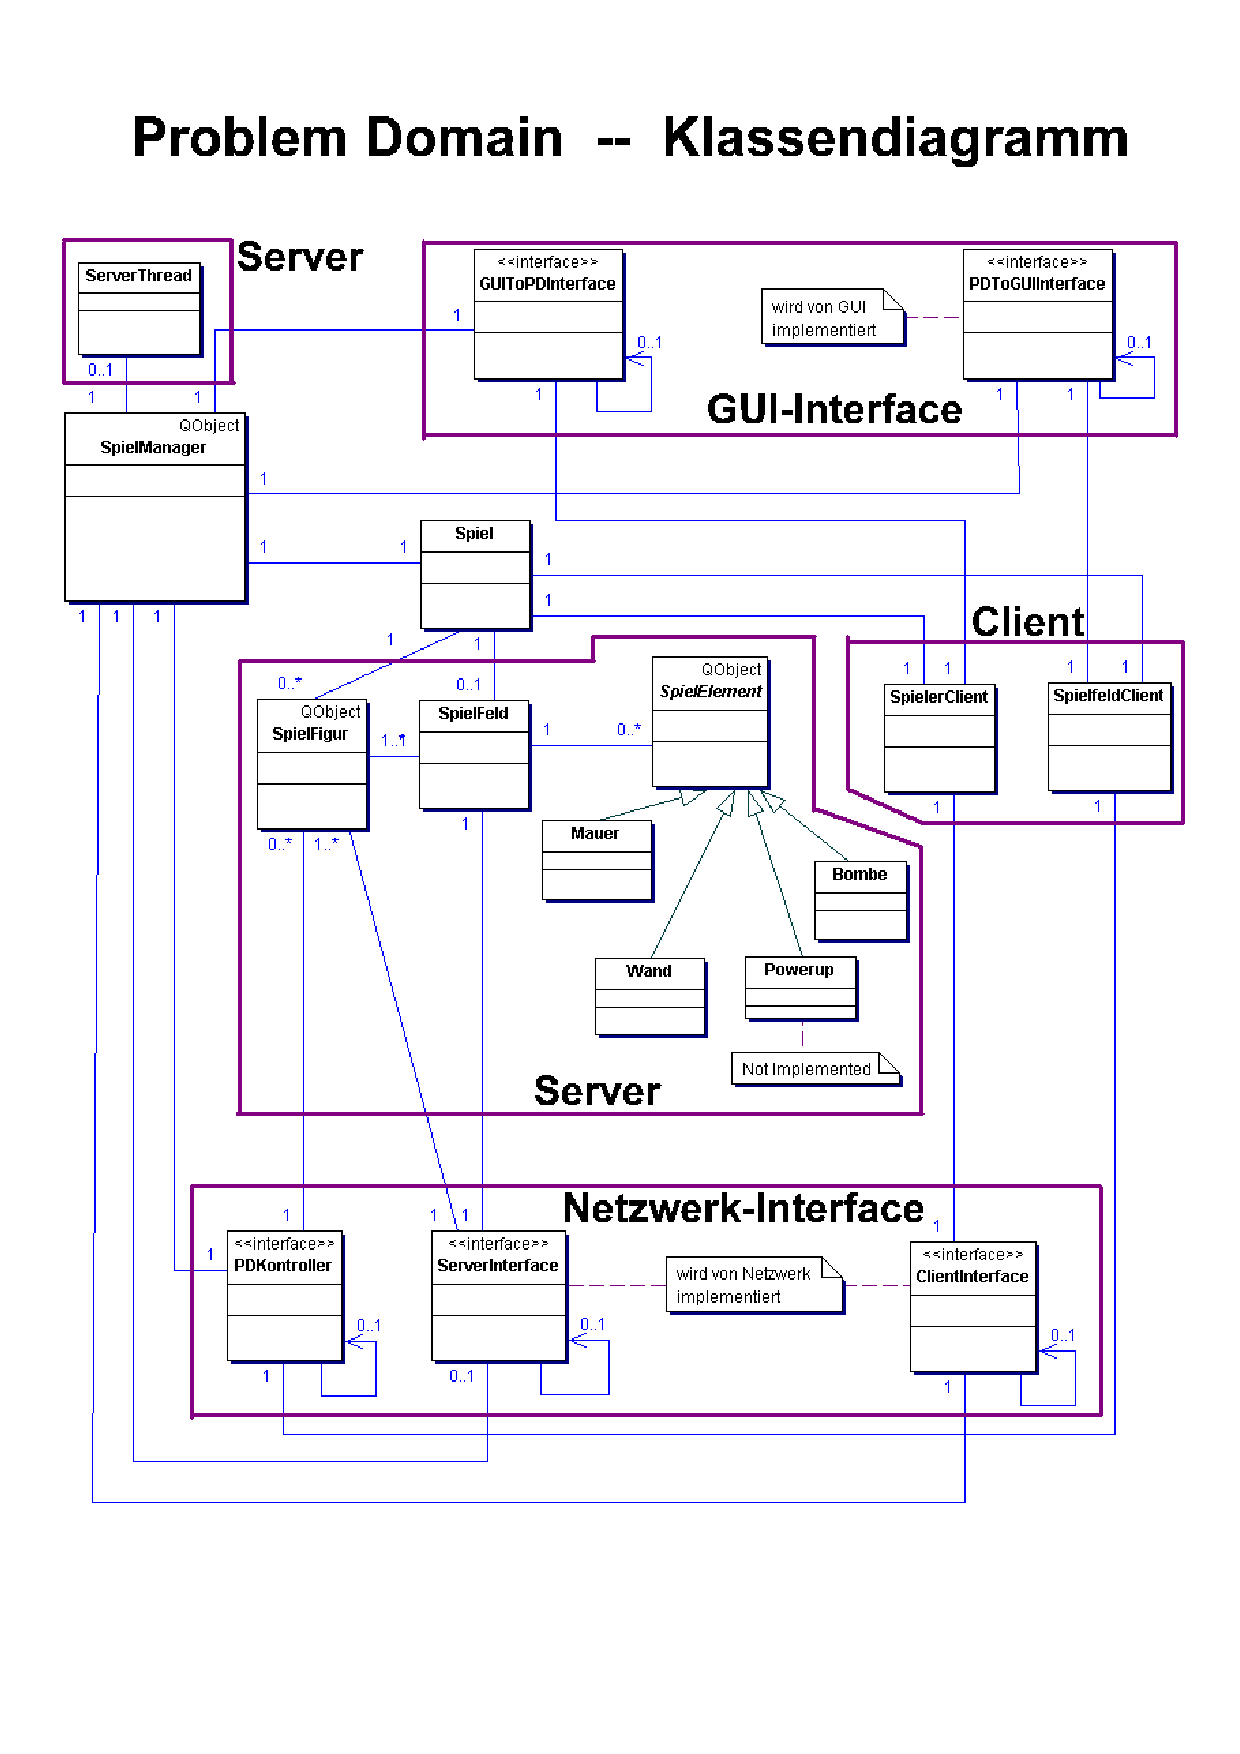
\includegraphics[height=18cm]{./images/pda4g.pdf}}
  \end{center}
  \caption{Klassendiagramm PD (siehe auch A3 Blatt in Register 9)}
\end{figure}

\section{PD Sequenzdiagramme}

\begin{figure}[H]
  \begin{center}
    {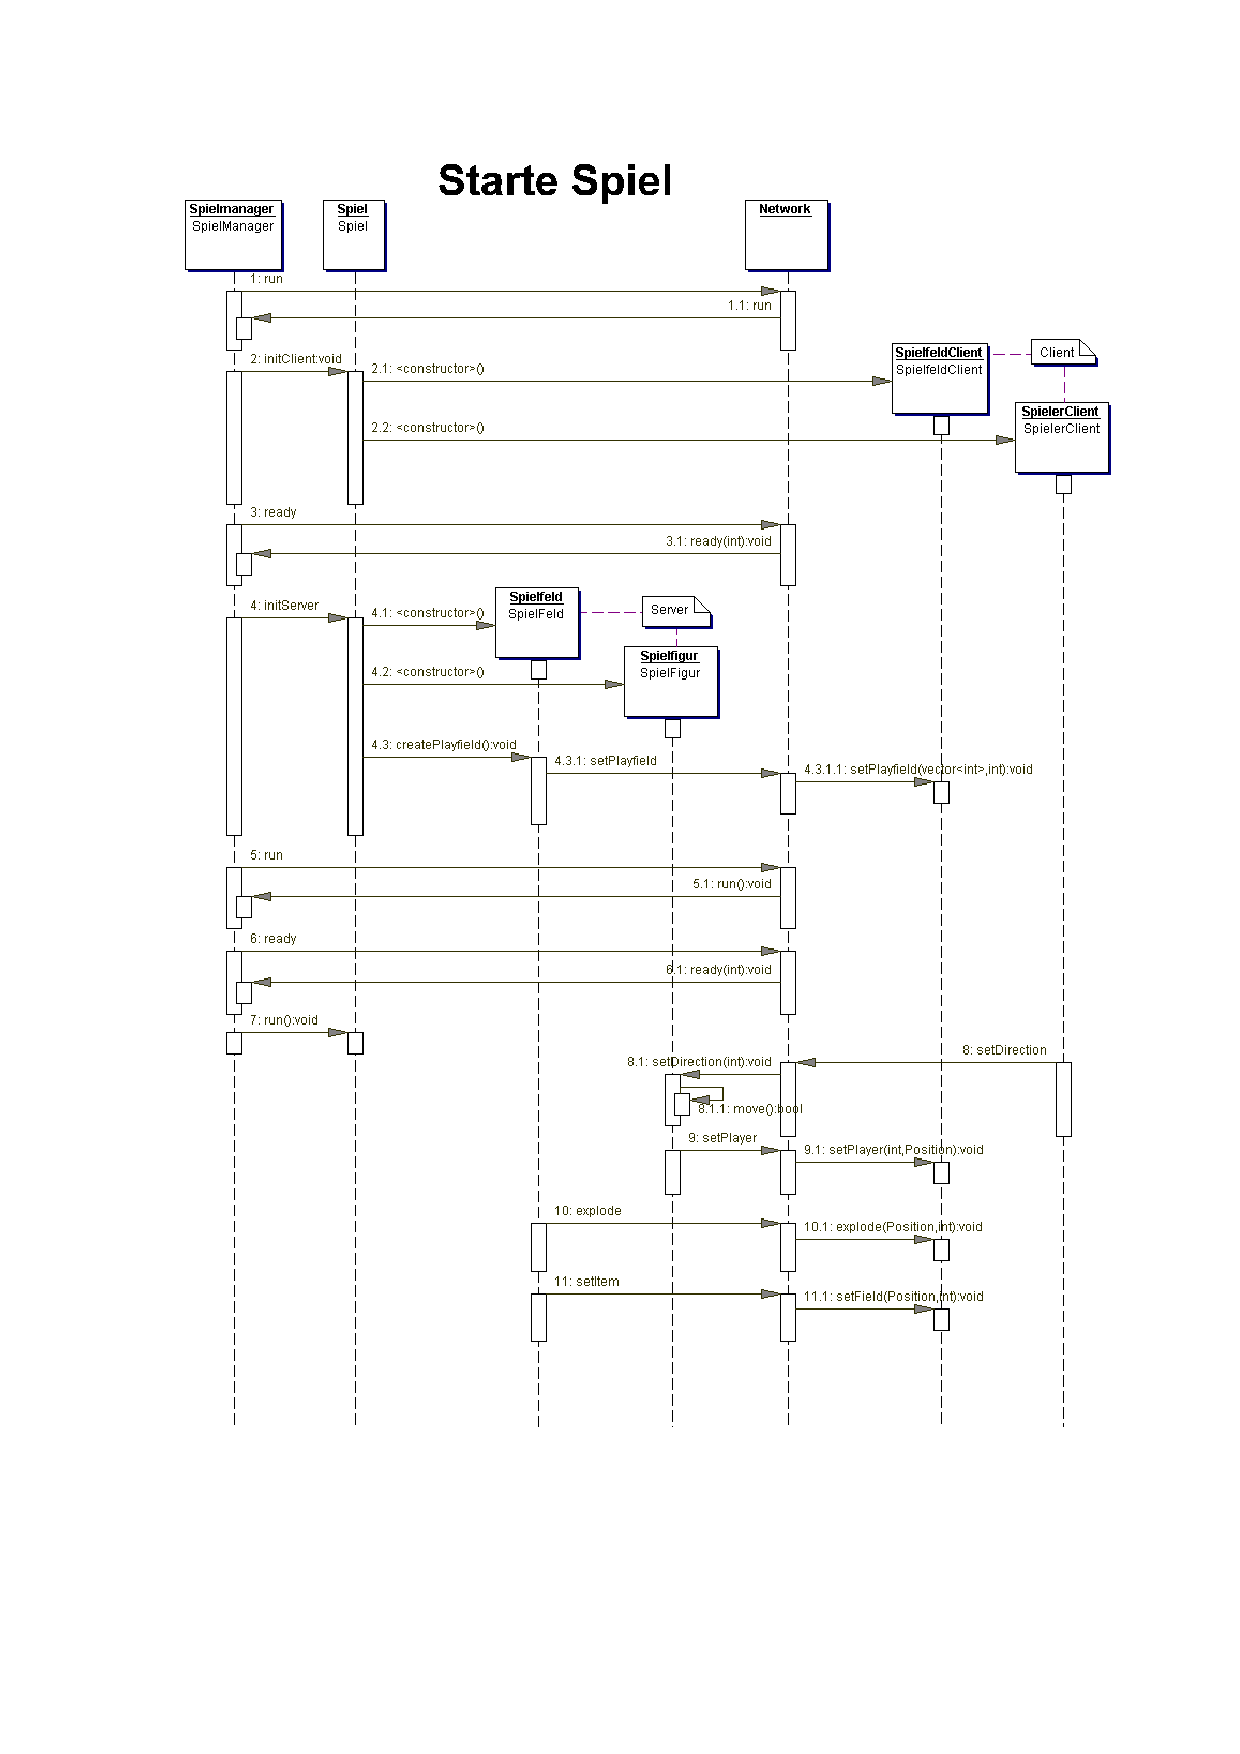
\includegraphics[height=18cm]{./images/startespiel2.pdf}}
  \end{center}
  \caption{Sequenzdiagramm f"ur neues Spiel}
\end{figure}

\begin{figure}[H]
  \begin{center}
    {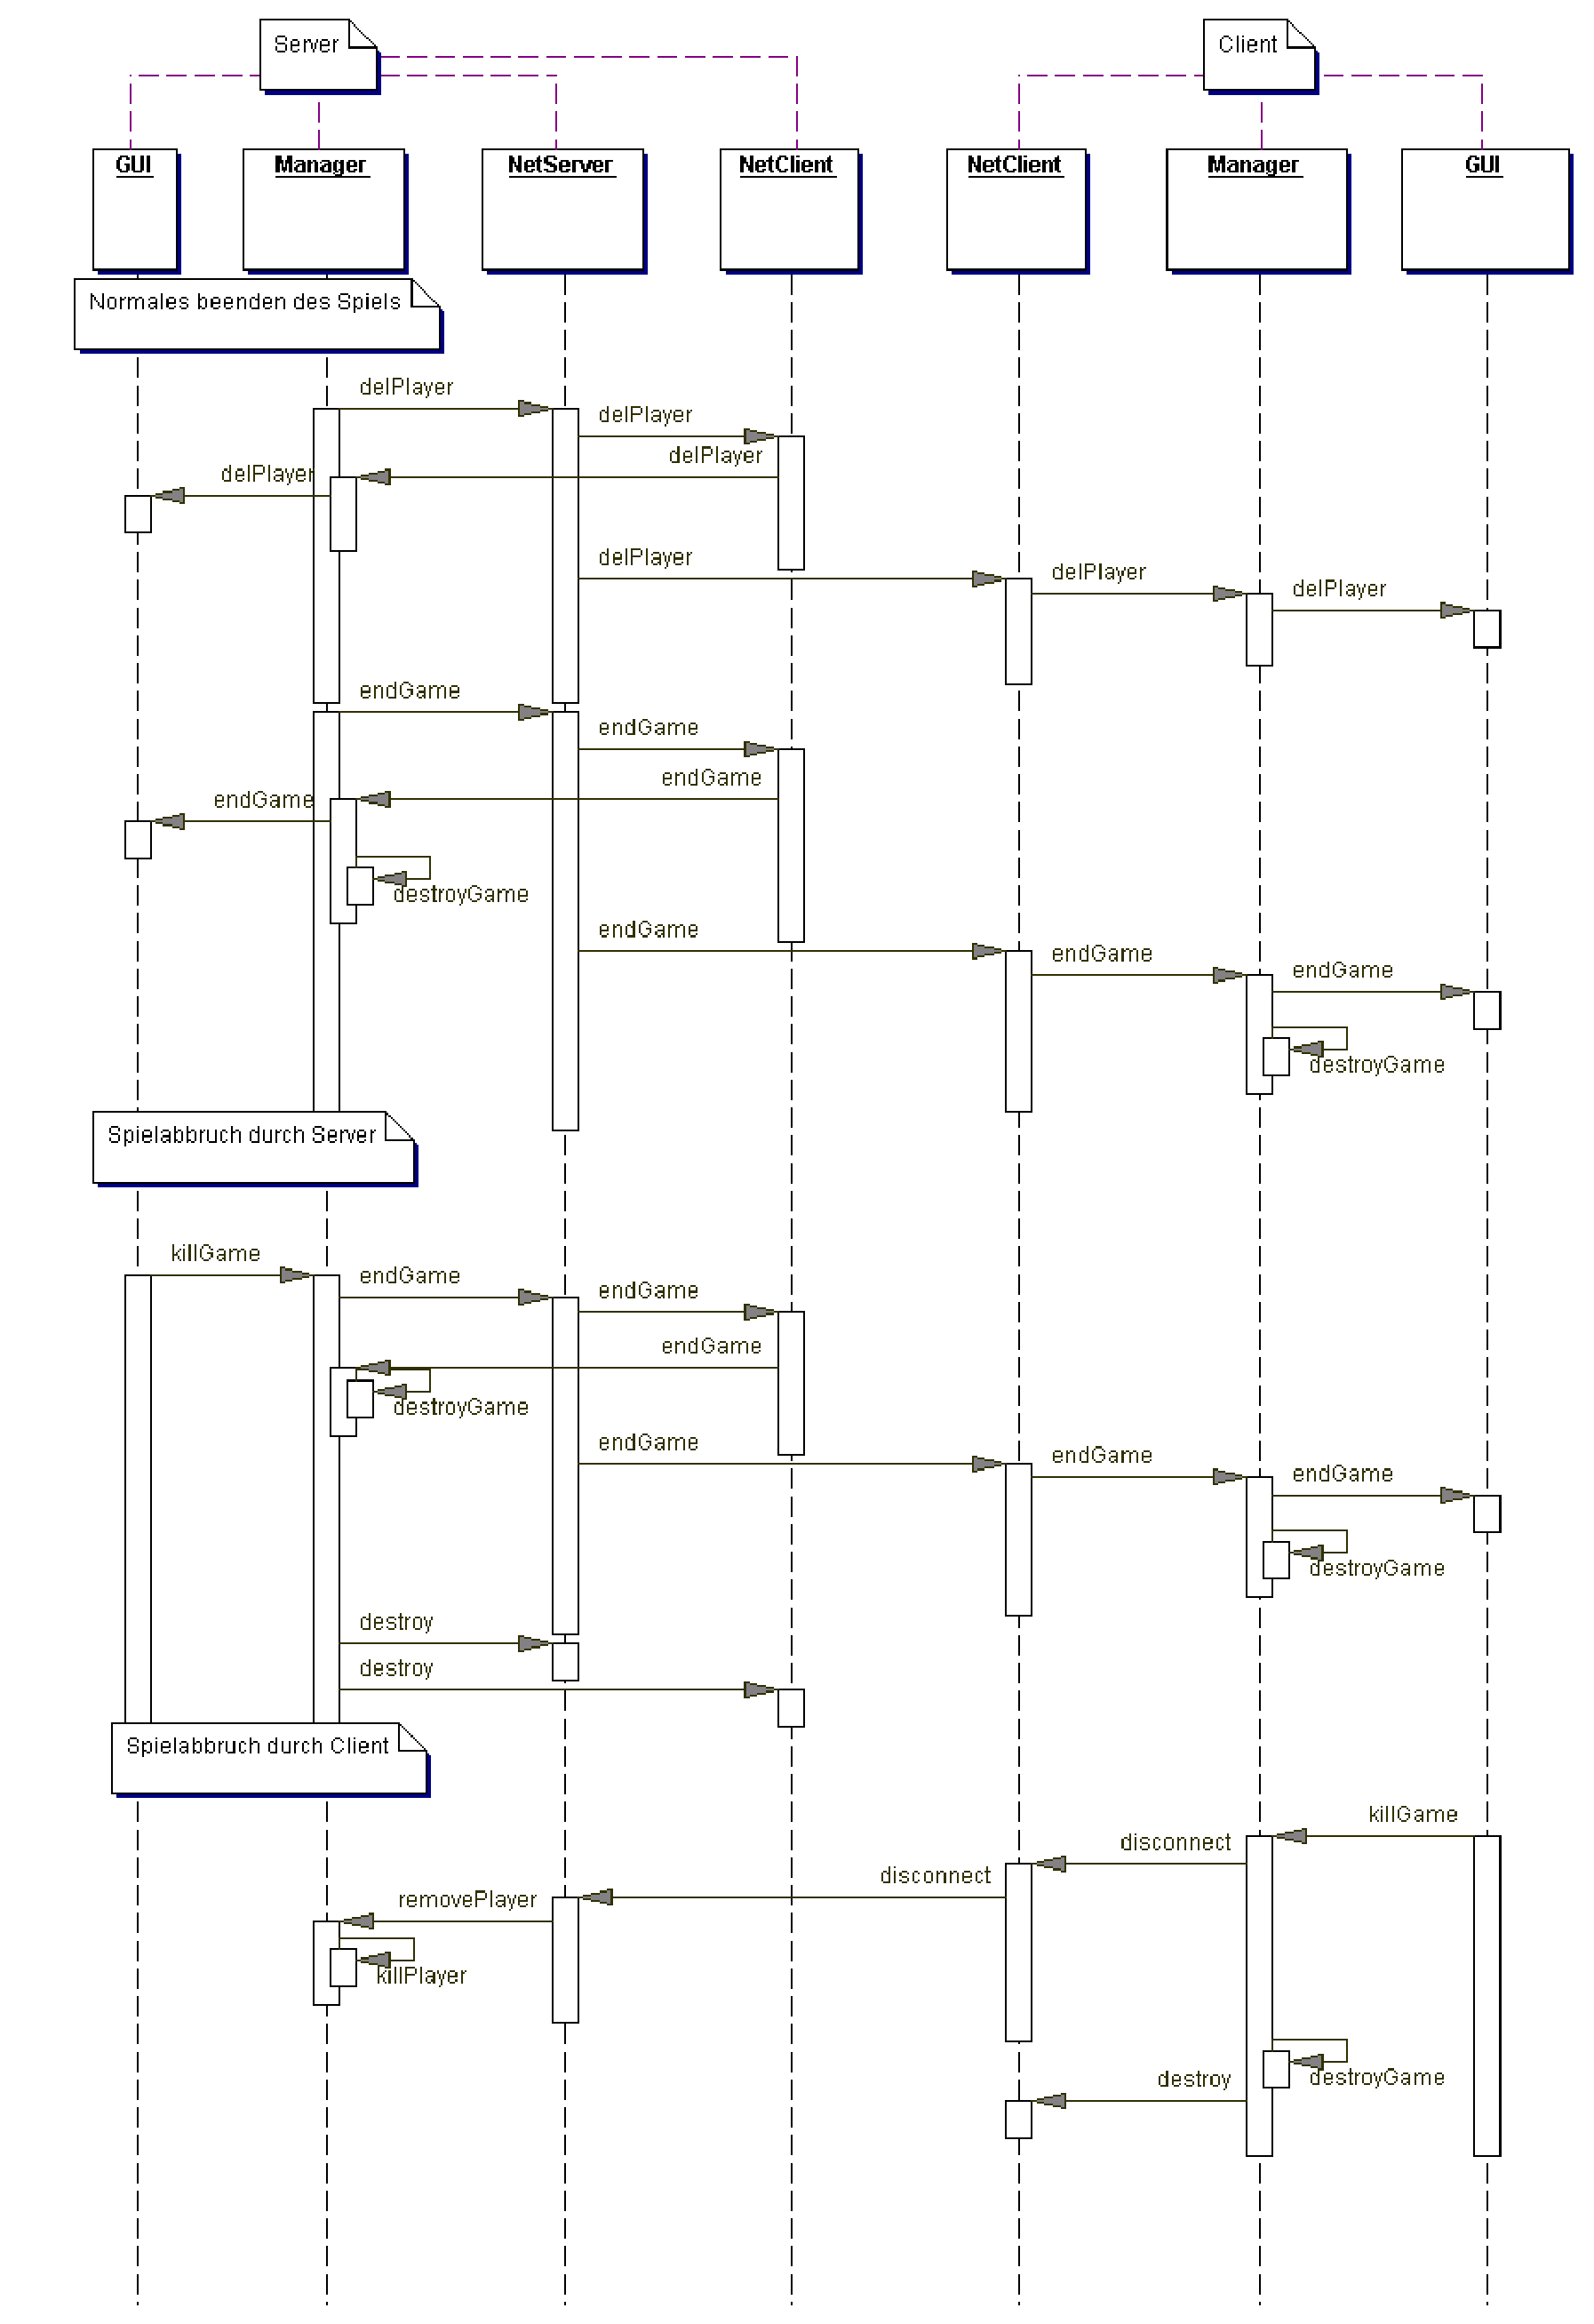
\includegraphics[height=18cm]{./images/endgame.pdf}}
  \end{center}
  \caption{Sequenzdiagramm f"ur das Beenden des Spiels}
\end{figure}

\begin{figure}[H]
  \begin{center}
    {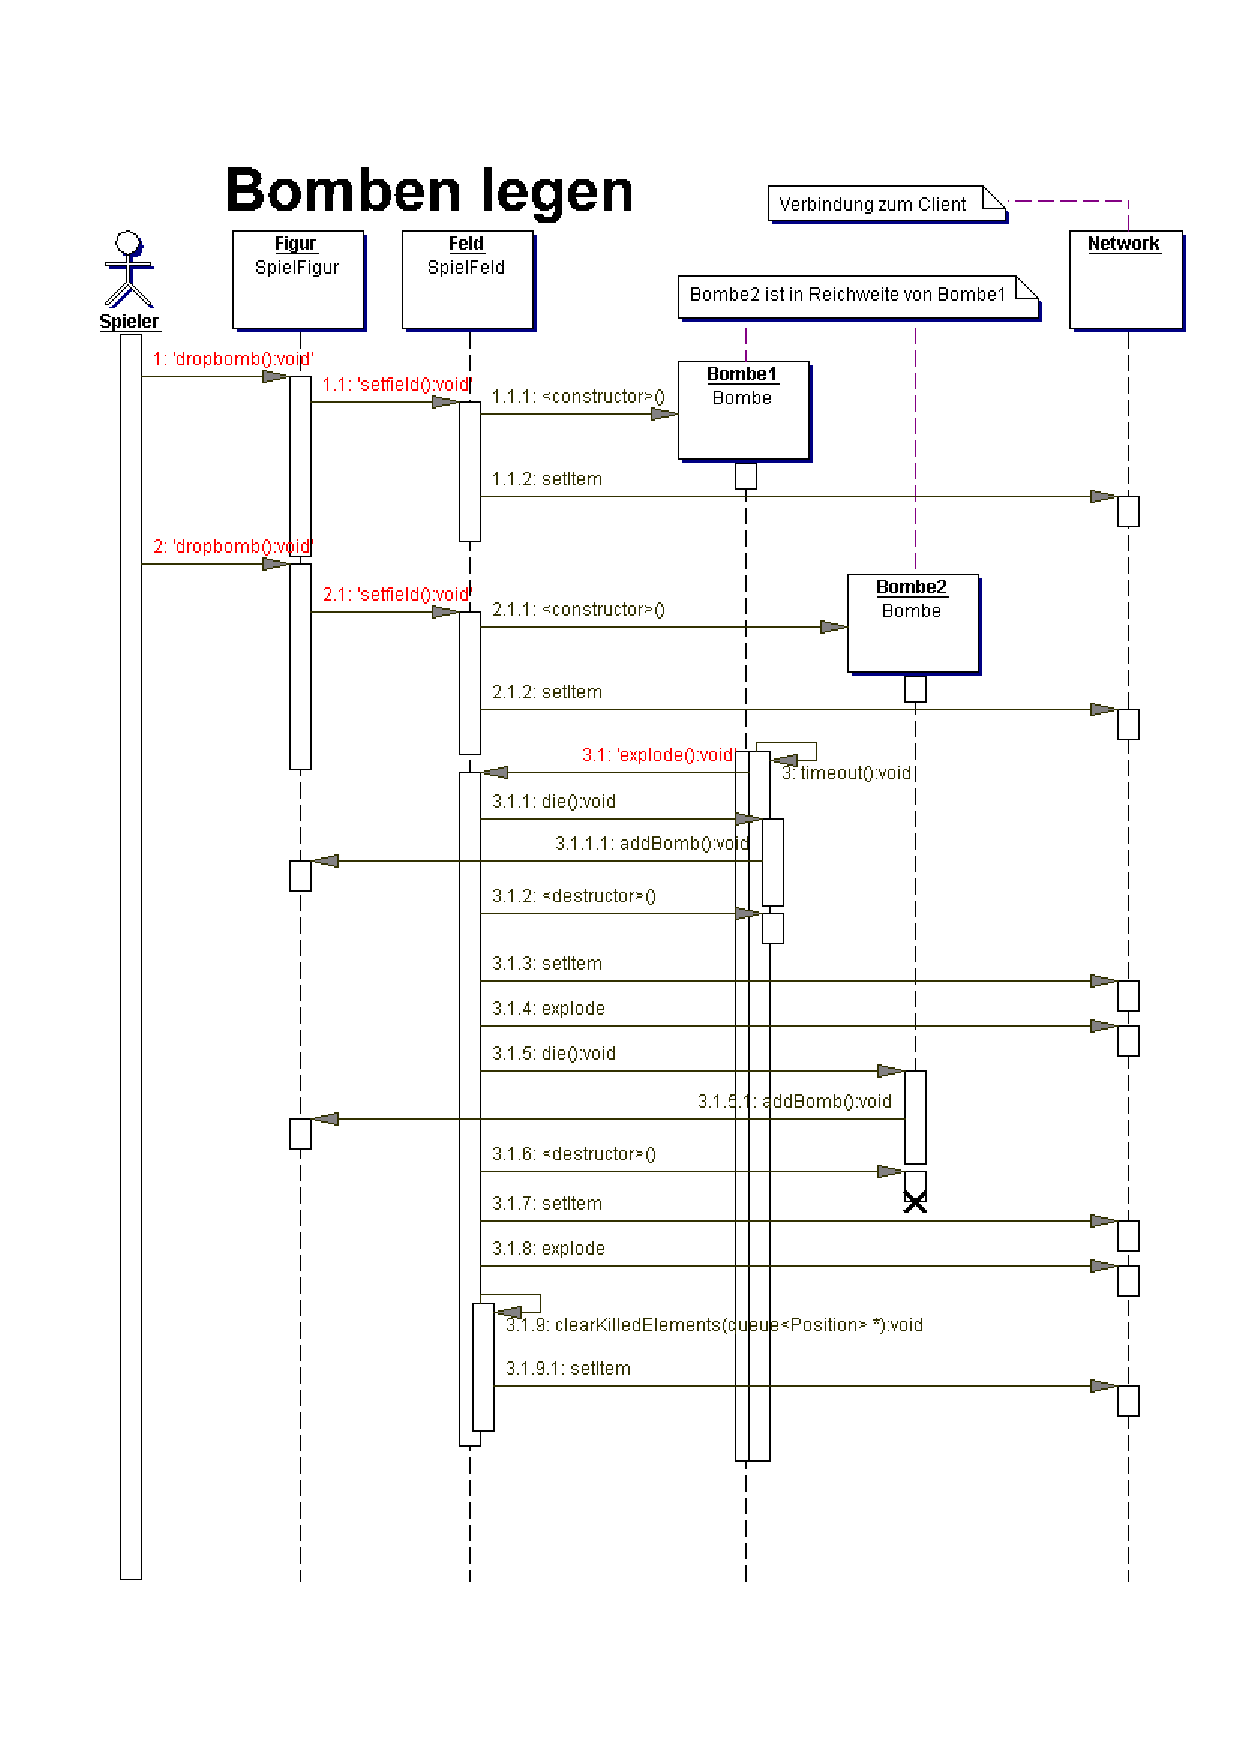
\includegraphics[height=18cm]{./images/bombenlegen.pdf}}
  \end{center}
  \caption{Sequenzdiagramm f"ur das Legen von Bomben}
\end{figure}

% ProblemDomain  Klassenbeschrieb
% 19.4.2002 U.Heimann   Dokument erstellt
% 26.4.2002 U.Heimann   erweitert, korrigiert
%  2.5.2002 U.Heimann   �nderung Client/Server
%  5.6.2002 u.Heimann   �nderung Iteration 2
% 12.7.2002 U.Heimann   Endversion

\section{PD Klassenbeschreibung}
Die endg"ultige Version des Spiels soll "uber ein Netzwerk gespielt werden. Deshalb wird die PD in Server und Client unterteilt.
Die Klassen des Servers sind f"ur die Berechnung des gesamten Spielverlaufs (Positionen, Treffererkennung, ...) verantwortlich.
Der Client konvertiert die Steuerbefehle und schickt sie "uber das Netzwerk an den Server. Der Server berechnet die Auswirkungen
und schickt die "Anderungen zur"uck an alle Clients. Der Client reicht die "Anderungen wiederum an das User Interface weiter.
Jeder Spieler hat auf seinem Rechner eine Instanz des Clients, aber nur einer hat zus"atzlich noch eine Instanz des Servers.

\subsection{Klasse SpielManager}
Der Spielmanager ist f"ur die Verwaltung des Spiels verantwortlich. Er kontrolliert den Verbindungsaufbau
und -abbruch der Clients und erzeugt die zum Spielen notwendigen Objekte.
\subsubsection{Attribute}
\begin{tabular}{p{50mm}p{90mm}}
-serverGame      : bool           &  True wenn dieser PC als Server agiert. \\
-playerConnected : bool[]         &  True wenn mit der entsprechenden ID ein Spieler verbunden ist. \\
-playerName      : string[]       &  Namen der verbundenen Spieler. \\
-playerReady     : bool[]         &  True wenn der Spieler zum Spielen bereit ist. \\
-game            : Spiel*         &  Pointer auf das Spiel-Objekt. \\
-serverThread    : ServerThread*  &  Pointer auf Server-Listening-Thread. \\
-pdMutex         : QMutex*        &  Mutex zum Schutz der PD vor Mehrfachzugriff. \\
-serverMutex     : QMutex*        &  Mutex zum Beenden des Server-Threads. \\
-client          : Client*        &  Pointer auf Client-Objekt, zum Abfragen des Sockets. \\
-clientTimer     : QTimer*        &  Timer zur regelm"assigen Abfrage des Client-Sockets. \\
 & \\
-guiInputInterface      : GUIToPDInterface*  &  Interface  GUI $\rightarrow$ PD \\
-guiOutputInterface     : PDToGUIInterface*  &  Interface  PD  $\rightarrow$ GUI \\
-netInputInterface      : PDKontroller*      &  Interface  NET $\rightarrow$ PD \\
-netOutClientInterface  : ClientInterface*   &  Interface  PD (client) $\rightarrow$ NET \\
-netOutServerInterface  : ServerInterface*   &  Interface  PD (server) $\rightarrow$ NET \\

\end{tabular}
\subsubsection{Funktionen}
\begin{tabular}{p{50mm}p{90mm}}
+startServer(string playerName)        : void  &  Startet den Netzwerk-Server und meldet sich als Spieler an. \\
+joinServer(string ipAddress, string playerName)  : void  &  Startet den Netzwerk-Client und meldet sich beim Server an. \\
+startGame()                           : void  &  Initialisiert und startet das Spiel mit den verbundenen Spielern. \\
+endGame()                             : void  &  Beendet das laufende Spiel. \\
+killGame()                            : void  &  Bricht das laufende Spiel ab. (zu irgendeinem Zeitpunkt) \\
+errorMsg(int msgNr, string addInfo)   : void  &  Bearbeitet Fehlermeldungen vom Netzwerk. \\
 & \\
+newPlayer(int playerID, string playerName) : void  &  Ein neuer Spieler hat sich beim Server angemeldet. \\
+removePlayer(int playerID)            : void  &  Entfernt einen Spieler aus der Spielerliste und entfernt ihn aus dem Spiel. \\
+ready(int playerID)                   : void  &  Setzt den Spieler spielbereit. \\
+distributeMsg(string info)            : void  &  Schickt eine Nachricht an alle verbundenen Clients weiter. \\
 & \\
+connectConfirm()                      : void  &  Best"atigt die Verbindung zum Server. \\
+setPlayerName(int playerID, string name) : void &  Setzt den Namen eines Verbundenen Spielers. \\
+disconnect()                          : void  &  Meldet sich beim Server ab. \\
+run()                                 : void  &  Synchronisiert und startet das Spiel. \\
+infoMsg(string info)                  : void  &  Zeigt eine Nachricht vom Server an. \\
 & \\
-createNetworkServer()                 : void  &  Startet den Server-Listening-Thread. \\
-killNetworkServer()                   : void  &  Beendet den Server-Listening-Thread. \\
-createNetworkClient()                 : void  &  Startet den Client-Timer zur Abfrage des Sockets. \\
-killNetworkClient()                   : void  &  Beendet den Client-Timer. \\
 & \\
-clientTimeout()                       : void  &  wird bei Ablauf des Client-Timers aufgerufen. \\
\end{tabular}


\subsection{Klasse Spiel}
Die Klasse Spiel erzeugt die restliche Spielstruktur (Spielfeld, Spielfiguren) je nach Anzahl
Spieler. Es wird immer ein Client erstellt, und beim Spielf"uhrer zus"atzlich noch ein Server. Sie ist daf"ur verantwortlich,
dass das Spiel mit allen Clients synchronisiert ist bevor das Spiel gestartet wird. \\
\subsubsection{Attribute}
\begin{tabular}{p{50mm}p{90mm}}
-serverFeld  :  Spielfeld*         &  Pointer auf das ServerSpielfeld. \\
-figur[4]    :  Spielfigur*        &  Pointer auf die Spielfiguren des Servers. \\
-clientFeld  :  SpielfeldClient*   &  Pointer auf das ServerSpielfeld. \\
-spieler     :  SpielerClient*     &  Pointer auf die Spielfigur des Clients. \\
\end{tabular}

\subsubsection{Funktionen}
\begin{tabular}{p{50mm}p{90mm}}
+initClient()             : void  &  Initialisiert die Client-Umgebung. \\
+initServer(bool activPlayers[], string playerNames[]) : void  &  Initialisiert die Server-Umgebung. \\
+ready()                  : bool  &  gibt TRUE zur"uck wenn Client bereit ist. \\
+run()                    : void  &  Synchronisiert und startet das Spiel. \\
+killPlayer(int playerID) : void  &  Entfernt einen Spieler vom Spielfeld. \\
-destroyClient()          : void  &  R"aumt die Client-Umgebung nach Spielende auf. \\
-destroyServer()          : void  &  R"aumt die Server-Umgebung nach Spielende auf. \\
\end{tabular}


\subsection{Klasse GUIToPDInterface (Singleton)}
"Uber diese Schnittstelle sendet das User Interface die Tastatureingaben des Spielers an die PD.\\
\subsubsection{Attribute}
\begin{tabular}{p{50mm}p{90mm}}
-manager : SpielManager*   &  Pointer auf den Spielmanager. \\
-spieler : SpielerClient*  &  Pointer auf den Spieler. \\
-pdMutex : QMutex*         &  Sichert die PD vor Mehrfachzugriff ab. \\
\end{tabular}
\subsubsection{Funktionen}
\begin{tabular}{p{50mm}p{90mm}}
+setManager(SpielManager* man, QMutex* pdMut) : void  &  Registriert den Spielmanager. \\
+setPlayer(SpielerClient* player): void  &  Registriert den Spieler. \\
+startServer(const char* player) : void  &  Startet neues Spiel als Server. \\
+joinServer(const char* ipAdress, const char* playerName) : void  &  Startet neues Spiel als Client. \\
+startGame()                     : void  &  Startet das Spiel mit den verbundenen Spielern (nur Server) \\
+killGame()                      : void  &  Beendet das Spiel zu einem beliebigen Zeitpunkt. \\
+keyPressed(int key)             : void  &  Eine Taste wurde gedr"uckt. \\
+keyReleased(int key)            : void  &  Eine Taste wurde losgelassen. \\
\end{tabular}

\subsection{Klasse PDToGUIInterface (Singleton)}
"Uber diese Schnittstelle sendet die PD die "Anderungen des Spielfeldes an das User Interface.
(siehe GUI) \\

\subsection{Klasse ServerInterface}
(siehe Netzwerk)

\subsection{Klasse ClientInterface}
(siehe Netzwerk)

\subsection{Klasse ServerThread}
Separater Thread f"ur die Abfrage des Server-Sockets. (Abgeleitet von QThread) \\
\subsubsection{Attribute}
\begin{tabular}{p{50mm}p{90mm}}
-runServer : QMutex*  &  Synchronisationsobjekt zum Beenden des Serverthreads. \\
-pdMutex   : QMutex*  &  Sichert die PD vor Mehrfachzugriff ab. \\
\end{tabular}
\subsubsection{Funktionen}
\begin{tabular}{p{50mm}p{90mm}}
+run()     : void     &  Ausf"uhrungsroutine des Threads. \\
\end{tabular}

\subsection{Klasse PDKontroller (Singleton)}
Der PDKontroller empf"angt und verarbeitet die Nachrichten vom Netzwerk. Sie ist als Singleton realisert und ist die Schnittstelle
vom Netzwerk zu der PD.
\subsubsection{Attribute}
\begin{tabular}{p{50mm}p{90mm}}
-spielManager : SpielManager*     &  Pointer auf den Manager. \\
-serverFigur  : Spielfigur*[]    &  Pointer auf die Spielfiguren (nur Server) \\
-clientFeld   : SpielfeldClient*  &  Pointer auf das Spielfeld. \\
\end{tabular}
\subsubsection{Funktionen}
\begin{tabular}{p{50mm}p{90mm}}
+setManager(SpielManager* manager) : void  &  Registriert den Spielmanager. \\
+setSpielfigur(int playerID, Spielfigur* figur) : void  &  Registriert eine Spielfigur. \\
+setClientFeld(SpielfeldClient* feld) : void  &  Registriert das Spielfeld. \\
Manager-Funktionen & \\
+newPlayer(int playerID, string playerName) : void  &  Ein neuer Spieler hat sich beim Server angemeldet. \\
+disconnect(int playerID)              : void  &  Ein Spieler hat sich abgemeldet. \\
+disconnect()                          : void  &  Der Server hat sich abgemeldet. \\
+ready(int playerID)                   : void  &  Der Spieler ist spielbereit. \\
+run()                                 : void  &  Spielstart  \\
+endGame()                             : void  &  Beendet das Spiel. \\
+connectConfirm()                      : void  &  Best"atigt die Verbindung zum Server. \\
+receiveMsg(string msg)                : void  &  Empf"angt eine Nachricht vom Server. \\
+receiveMsg(int playerID, string msg)  : void  &  Empf"angt eine Nachricht vom Client (zum Verteilen an alle Clients). \\
+errorMsg(int msgNumber, string addInfo) : void  & Empf"angt eine Fehlermeldung vom Netzwerk. \\
+setPlayerName(int playerID, string name) :  &  Setzt den Namen eines Spielers. \\
Server-Funktionen & \\
+setDirection(int direction, int playerID) : void  &  Setzt neue Laufrichtung des Spielers. \\
+setBombPressed(bool keypressed, int playerID) : void   &  Setzt das Bomben-lege-Flag. \\
Client-Funtionen & \\
+setPlayfield(vector<int> feldinfo, int zeilenbreite) : void  &  Initialisiert das ganze Spielfeld. \\
+setItem(Position position, int item) : void  &  Setzt ein einzelnes Objekt auf dem Spielfeld. \\
+setPlayer(int playerID, Position position) : void  &  Setzt die Position einer Spielfigur. \\
+delPlayer(int playerID) : void  &  L"oscht einen Spieler vom Spielfeld. \\
+explode(Position position, int reichweite) : void  &  L"ost eine Explosion auf dem Spielfeld aus. \\
\end{tabular}


\subsection{Klasse Spielfeld}
Die Klasse Spielfeld enth"alt ein Array das den aktuellen Zustand und die Positionen aller Spielelemente representiert. Sie hat
Zugriff auf alle spielentscheidenden Informationen. \\
\subsubsection{Attribute}
\begin{tabular}{p{50mm}p{90mm}}
-feld         : Spielelement*[]         &  Abbild des aktuellen Spielstandes. Jeder Eintrag im Array entspricht einem Feld. d.h.
                                           es k"onnen nicht mehrere Elemente auf einem Feld sein. (Spielfiguren werden hier
                                           nicht gespeichert!) \\
-player       : Spielfigur[]            &  Zeigerliste auf alle Spielfiguren des aktuellen Spiels. Die Position der Figur ist
                                           bei der Figur gespeichert.\\
-game         : Spiel*                  &  Pointer auf das Spiel-Objekt. \\
-netInterface : ServerInterface*        &  Pointer zum Netzwerk-Interface des Servers. \\
-minPlayers   : int                     &  Sind weniger Spieler als minPlayers auf dem Feld wird das Spiel beendet. \\
\end{tabular}
\subsubsection{Funktionen}
\begin{tabular}{p{50mm}p{90mm}}
+startGame() : void  &  Startet das Spiel. \\
+stopGame() : void  &  Beendet das Spiel. \\
+setField(Position pos, int item, Spielfigur* figur = NULL) : void  &  Setzt ein bestimmtes Element an die Koordinate (x,y). \\
+getField(Position pos) : int item        &  Liefert das Element das sich an der Koordinate (x,y) befindet. \\
+setPlayer(int playerID, Spielfigur* player) : void     &  Meldet einen neuen Spielfigur beim Spielfeld an. \\
+delPlayer(int playerID) : void  &  Meldet den Spieler ab. \\
+explode(Position pos, int reichweite, queue<Position>* toDie = NULL) : void  &  Berechnet die Explosion. \\
-clearKilledElements(queue$<$Position$>$* toDie) : void  &  L"oscht die gesprengten Elemente vom Spielfeld. \\
\end{tabular}

\subsection{Klasse Spielfigur}
Die Klasse Spielfigur enth"alt alle wichtigen Informationen "uber Position und Zustand der Spielfigur. \\
\subsubsection{Attribute}
\begin{tabular}{p{50mm}p{90mm}}
-spielfeld     : Spielfeld*       &  Pointer auf das Spielfeld-Objekt. \\
-pdKontroller  : PDKontroller*    &  Pointer auf den den PD-Kontroller. F"ur ankommende Meldungen vom Netzwerk. \\
-netInterface  : ServerInterface* &  Pointer auf das Netzwerk-Interface. F"ur abgehende Meldungen ans Netzwerk. \\

-playerID      : int       &  Spielernummer  \\
-playerName    : string    &  Name des Spielers. \\
-position      : Position  &  Position der Spielfigur auf dem Spielfeld in (x,y) Koordinaten. \\
-direction     : int       &  Richtung in die die Spielfigur gehen m"ochte. (STAY, UP, DOWN, LEFT, RIGHT) \\
-numberOfBombs : int       &  Die Anzahl Bomben die er noch legen darf. -1 wenn Bombe gelegt wurde, +1 wenn seine Bombe explodiert ist
                              oder ein Bomben-Powerup aufgenommen wurde. \\
-reichweite    : int       &  Reichweite der Bombe in Feldern. Wird der Bombe "ubergeben wenn sie gelegt wird. Wird erh"oht, wenn ein
                              Flammen-Powerup aufgenommen wird. \\
-alive         : bool      &  TRUE wenn die Spielfigur noch lebt. \\
-bombPressed   : bool      &  TRUE wenn die Bomben-lege-Taste gedr"uckt ist. \\
-moveTimer     : QTimer*   &  Timer f"ur die Bewegungs-Verz"ogerung. \\
\end{tabular}
\subsubsection{Funktionen}
\begin{tabular}{p{50mm}p{90mm}}
+setDirection(int dir)          : void   &  Setzt die Laufrichtung der Spielfigur (STAY, UP, DOWN, LEFT, RIGHT). \\
+setBombPressed(bool bomb)      : void   &  Setzt das bombPressd Flag (bomben-lege-Taste gedr"uckt). \\
+getName()                      : string &  Liefert den Namen des Spielers. \\
+getPosition()                : Position &  Liefert die aktuelle Position der Spielfigur. \\
+addBomb()                      : void   &  F"ugt eine Bombe zum Arsenal der Spielfigur hinzu. \\
+wakeup()                       : void   &  Erweckt die Spielfigur zum Leben, erlaubt ihr sich zu bewegen. \\
+die()                          : void   &  Zerst"ort die Spielfigur wenn sie gesprengt wurde. \\
+move()                         : bool   &  Bewegt die Spielfigur um ein Feld in die aktuelle Richtung (direction). \\
+getReichweite()                : int    &  Gibt die Reichweite zur"uck. \\
-dropBomb()                     : void   &  Legt eine Bombe an der aktuellen Position sofern noch Bomben im Arsenal. \\
-checkField(int posx, int posy) : int    &  Pr"uft ob ein Feld auf dem Spielfeld passierbar ist oder nicht. \\
-timerDone()                    : void   &  Wird aufgerufen wenn der moveTimer abgelaufen ist. \\
\end{tabular}

\subsection{Klasse SpielerClient}
Die Klasse Spieler empf"angt die Benutzereingaben, bestimmt die daraus folgenden Aktionen und leitet sie an den Server weiter.\\
\subsubsection{Attribute}
\begin{tabular}{p{50mm}p{90mm}}
-guiInterface : GUIToPDInterface*  &  Pointer zum GUI-Interface, zum Empfang der Benutzereingaben. \\
-netInterface : ClientInterface*   &  Pointer zum Netzwerk-Interface, zum Versenden der Aktionen. \\
-keylist      : bool[5]            &  Speichert die Informationen welche Tasten momentan gedr"uckt sind. \\
-oldDirection : int                &  Die zuletzt "ubermittelte bewegungsrichtung. \\
\end{tabular}
\subsubsection{Funktionen}
\begin{tabular}{p{50mm}p{90mm}}
+keyPressed(int key) : void      &  Eine Taste wurde gedr"uckt. \\
+keyReleased(int key) : void     &  Eine Taste wurde losgelassen. \\
-computeDirection() : void       &  Berechnet die Laufrichtung aus den Daten der keylist und sendet sie an den Server. \\
\end{tabular}

\subsection{Klasse SpielfeldClient}
Die Klasse SpielfeldClient hat ein vereinfachtes Abbild der Spielsituation gespeichert. Sie ben"otigt dieses zur
berechnung der Explosionen. Sie empf"angt alle "Anderungen vom Server und gibt sie ans GUI weiter.\\
\subsubsection{Attribute}
\begin{tabular}{p{50mm}p{90mm}}
-guiInterface   : PDToGUIInterface*  &  Pointer zum GUI-Interface, zum Senden der "Anderungen. \\
-pdKontroller   : PDKontroller*      &  Pointer zum PD-Kontroller, zum Empfangen der Spielfeld"anderungen. \\
-field          : int[][]            &  Vereinfachtes Abbild der Spielsituation. \\
-playerPosition : Position[4]        &  Die Positionen der Spieler auf dem Spielfeld. \\
-readySet       : bool               &  TRUE wenn bereit zum spielen. \\
\end{tabular}
\subsubsection{Funktionen}
\begin{tabular}{p{50mm}p{90mm}}
+setPlayfield(vector<int> feldinfo, int zeilenbreite) :  void  &  Setzt das gesamte Spielfeld. \\
+setField(Position pos, int item)       : void  &  Setzt ein bestimmtes Element an die Koordinate (x,y). \\
+setPlayer(int playerID, Position pos)  : void  &  Setzt die Spielfigur (nr) an die Position (x,y). \\
+delPlayer(int playerID)                : void  &  L"oscht einen Spieler vom Spielfeld. \\
+explode(Position pos, int reichweite)  : void  &  berechnet eine Explosion. \\
\end{tabular}

\subsection{Klasse SpielElement}
Oberklasse aller auf dem Spielfeld platzierbaren Elemente wie Mauer, Wand, Bombe und Powerup (ausser den Spielfiguren). \\
\subsubsection{Attribute}
\begin{tabular}{p{50mm}p{90mm}}
-position    : Position  &  Position des Elements. \\
-elementType : int       &  Typ des Elements. \\
\end{tabular}
\subsubsection{Funktionen}
\begin{tabular}{p{50mm}p{90mm}}
+die()     : SpielElement*  &  Rein Virtuelle Funktion die beim sprengen des Objekts aufgerufen wird. \\
+getType() : int            &  Liefert den Typ des Elements. \\
\end{tabular}

\subsection{Klasse Mauer}
Die Mauer ist vom Spielelement abgeleitet. Sie kann durch eine Explosion nicht zerst"ort werden. Sie hat keine
spezielle Funktionalit"at.\\

\subsection{Klasse Wand}
Die Wand ist vom Spielelement abgeleitet. Sie kann durch eine Explosion zerst"ort werden und erzeugt dabei ev. ein Powerup. \\
\subsubsection{Attribute}
\begin{tabular}{p{50mm}p{90mm}}
-powerupType : int  &  Typ des versteckten Powerups. \\
\end{tabular}
\subsubsection{Funktionen}
\begin{tabular}{p{50mm}p{90mm}}
+getPowerupType() : int  &  Liefert den Typ des versteckten Powerups. \\
\end{tabular}

\subsection{Klasse Bombe}
Die Bombe ist vom Spielelement abgeleitet. Beim Erzeugen startet der Timer, der am Ende eine Explosion und damit
die Zerst"orung der Bombe einleitet. Sie kann durch eine Explosion zerst"ort werden und explodiert dabei selbst. \\
\subsubsection{Attribute}
\begin{tabular}{p{50mm}p{90mm}}
-dropper      : Spielfigur*  &  Pointer auf die Spielfigur die sie erzeugt hat. \\
-playfield    : Spielfeld*   &  Pointer auf das Spielfeld auf dem sie liegt. \\
-explodeTimer : QTimer*      &  Timer zur Verz"ogerung der Explosion. \\
-reichweite   : int          &  Die Reichweite der Explosion, wird beim Erzeugen gesetzt. \\
\end{tabular}
\subsubsection{Funktionen}
\begin{tabular}{p{50mm}p{90mm}}
+getReichweite() : int   &  Liefert die Reichweite der Bombe. \\
-timeout()       : void  &  wird vom Timer aufgerufen wenn er abgelaufen ist. L"ost die Explosion aus. \\
\end{tabular}


%end pd design

% Begin Netzwerk Interface  Design
\section{Netzwerk Interface}

\begin{figure}[H]
  \begin{center}
    {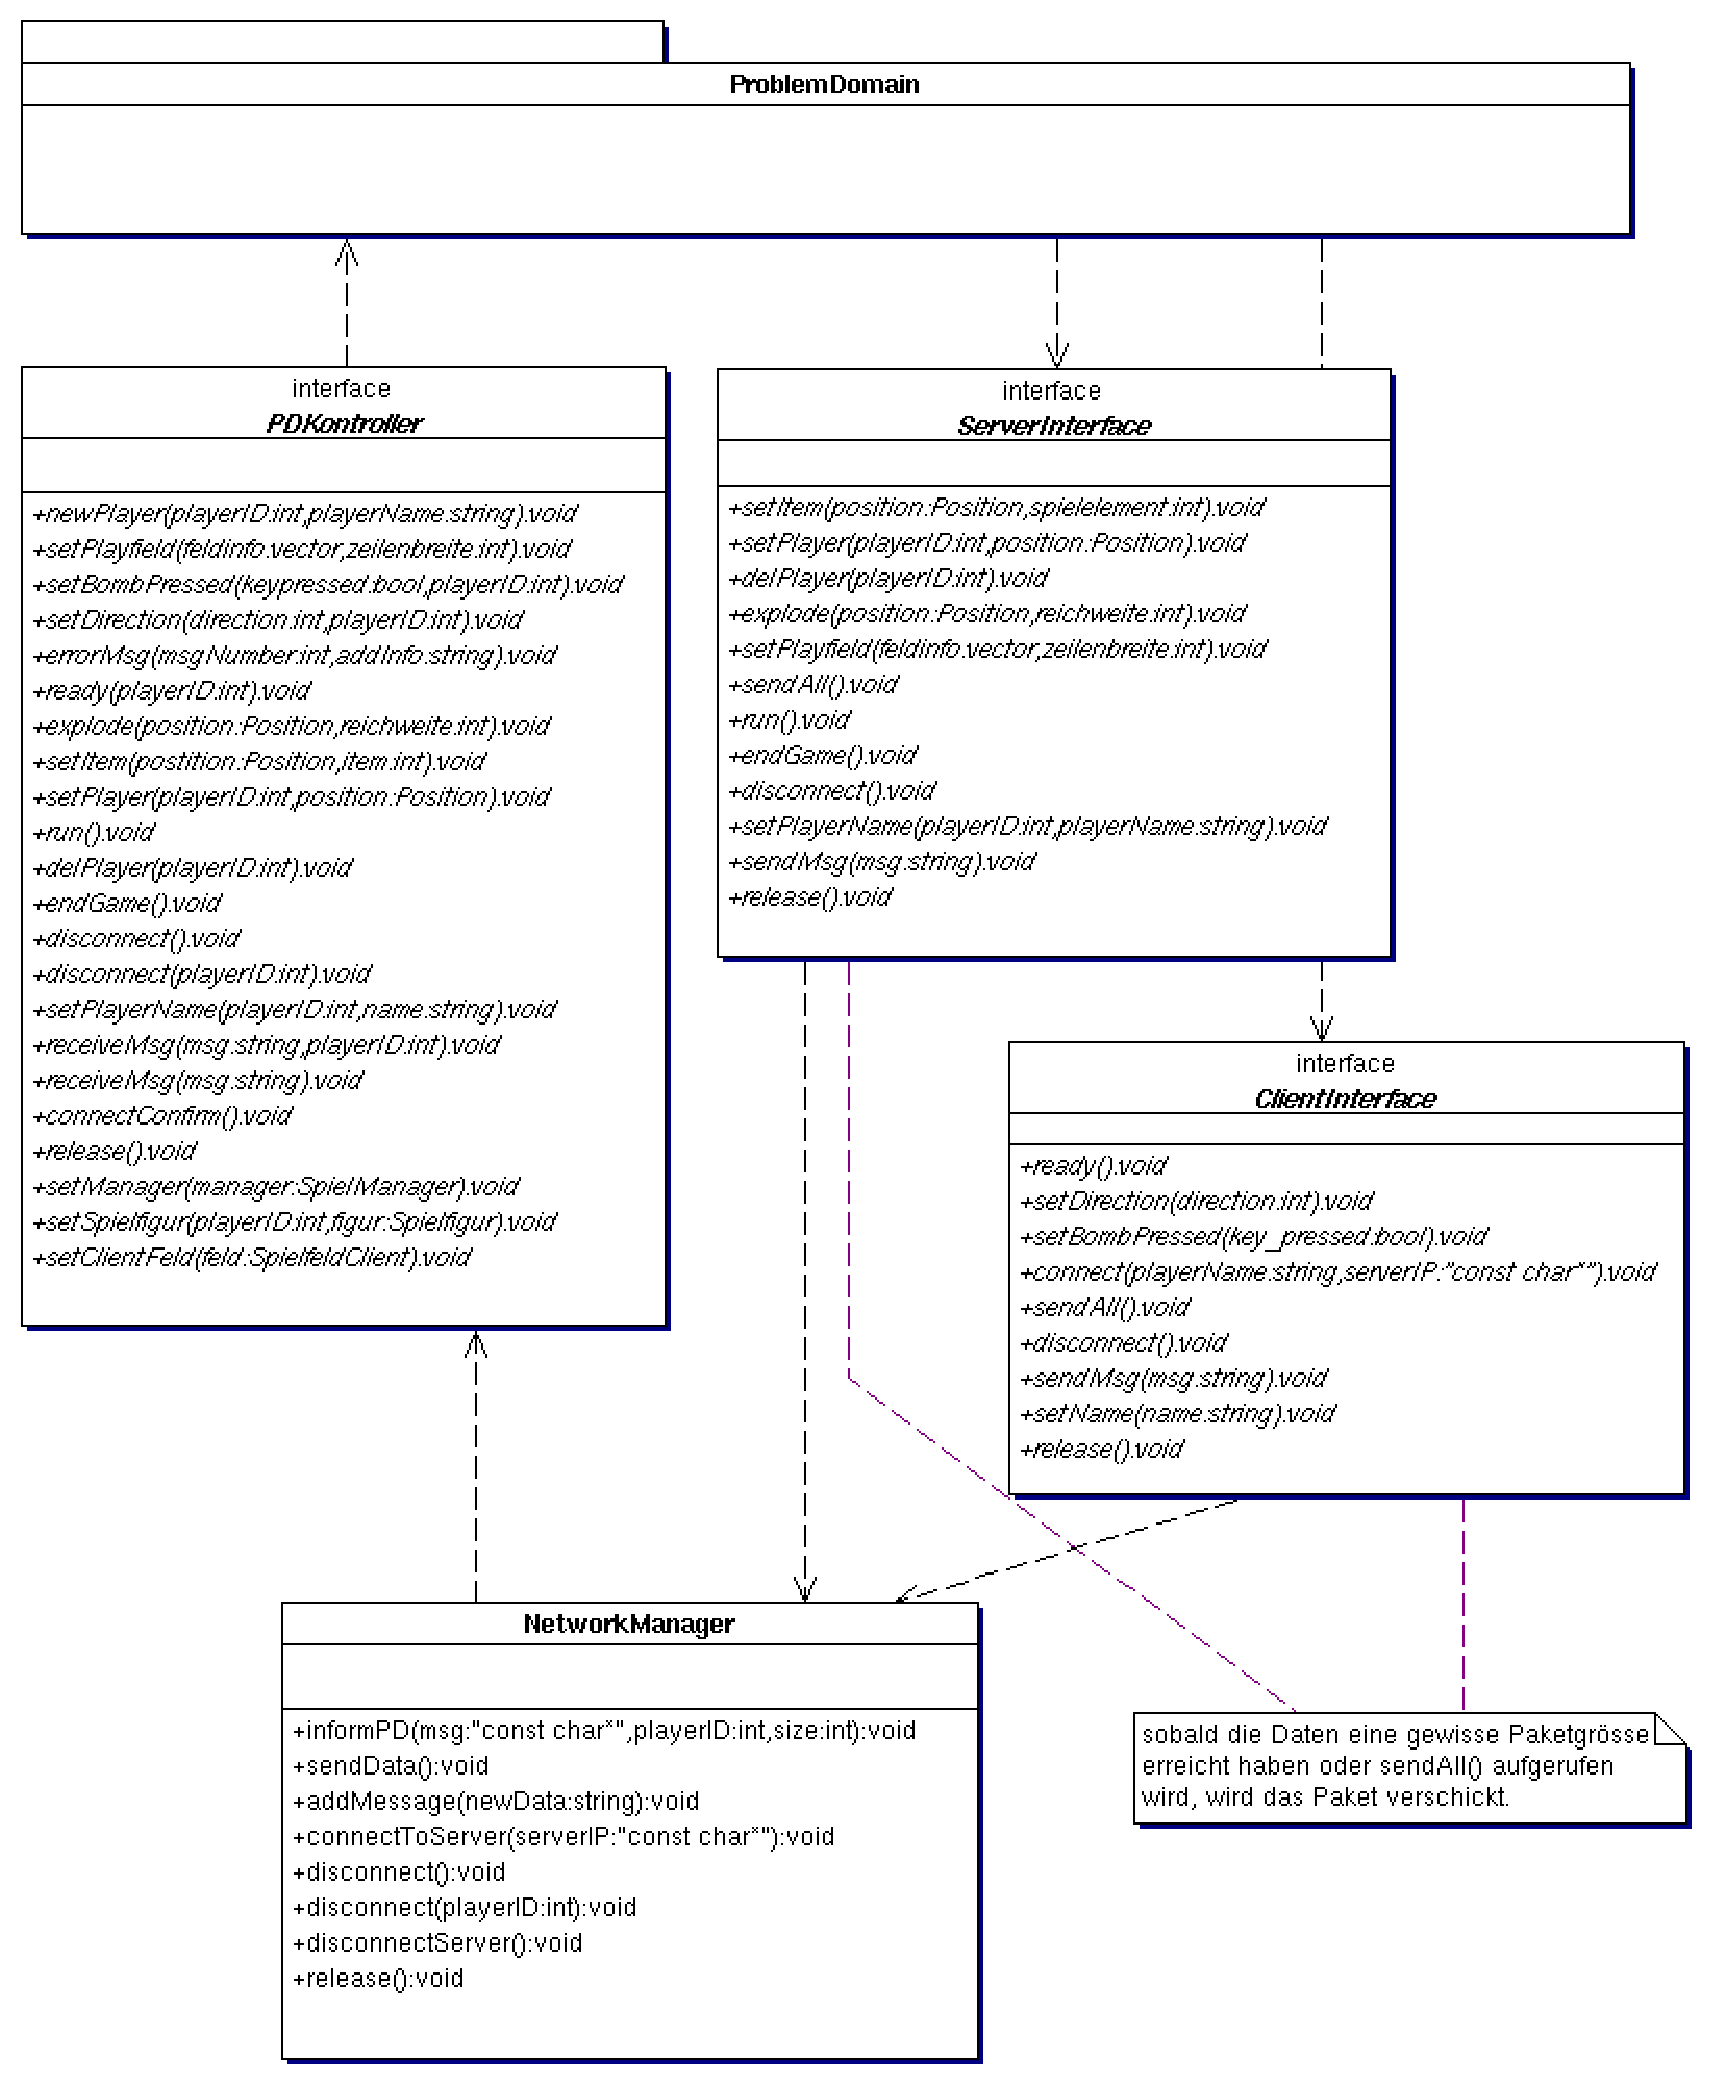
\includegraphics[height=20cm]{./images/netinterface.pdf}}
  \end{center}
  \caption{Interface zwischen Problem Domain und Netzwerk}
\end{figure}

Der Problem Domain stehen die als Singleton implementierten Klassen ServerInterface
und Clientinterface zur Verf"ugung. Die Problem Domain eines Servers verwendet ausschliesslich
das ServerInterface, um mit allen mitspielenden Clients zu kommunizieren. \\
Die Problem Domain eines Clients benutzt das ClientInterface, um sich bei dem Spielserver
anzumelden und ihm Ereignisse zu melden.\\
Die Klassen ServerInterface und ClientInterface rufen ihrerseits Methoden 
der Klasse NetworkManager auf, welcher mit dem Netzwerk kommuniziert. 
Der NetworkManager wird von der Netzwerkschicht aufgerufen und ruft selbst Methoden aus
der Klasse PDKontroller auf.\\
Die Schnittstelle generiert einen tempor"aren String der verschiedene Protokollmessages 
enth"alt. Welche Protokollmessages eingepackt werden ist davon abh"angig, welche Methoden
des Serverinterfaces oder des Clientinterfaces aufgerufen wurden.\\
Dieses Paket wird abgeschickt, sobald es eine gewisse L"ange erreicht hat, oder die Problem Domain
dies durch einen Methodenaufruf ausl"ost.

\section{Netzwerk Interface Klassenbeschreibung}

Verwendete Konstante aus global.h zur Konfiguration des Verhaltens der Schnittstelle:
\\MAX\_STRING\_PAKET\_SIZE. "Ubersteigt der tempor"ar angelegte String der die Nutzdaten 
enth"alt diese L"ange, wird er nach dem Einpacken der letzten Protokollmessage automatisch
verschickt. Zum sofortigen Versenden der Daten kann sowohl im Serverinterface als auch im
Clientinterface die Methode sendAll() aufgerufen werden.
Als Singleton enth"alt diese Klasse auch eine Methode getServerInterface die einen Pointer
auf die Schnittstelle zur"uckgibt.

\subsection{Klasse ServerInterface}
Diese Klasse wird von der Problem Domain des Spielservers benutzt, um Informationen an alle
Spielclients zu schicken. 
Sie ist nach dem Singleton Pattern implementiert.

\subsubsection{Funktionen}
\begin{tabular}{p{50mm}p{90mm}}
+setItem(Position \_pos,int spielelement):void 		 &ein einzelnes Spielelement wird platziert\\
+setPlayer(int playerID, Position \_pos):void 		 &die Spielfigur eines Spielers wird plaziert\\
+delPlayer(int playerID):void;				 &ein Spieler wird aus dem Spiel entfernt\\
+explode(Position \_pos,int reichweite):void		 &signalisiert den Spielclients das Explodieren einer Bombe\\
+setPlayfield(vector$<$int$>$ feldinfo,int zeilenbreite):void&verschickt Spielfelddaten; feldinfo enth"alt Spielelemente;
							  zeilenbreite gibt die Anzahl Felder in einer Horizontalen
							  des Spielfeldes an\\
+sendAll():void 				 	 &l"ost das Versenden des zusammengesetzten Datenpaketes aus\\
+getServerInterface(): ServerInterface*		         &gibt eine Instanz des Serverinterfaces zur"uck\\
+run():void &Startet das Spiel auf den Clients\\
+endGame():void &Signalisiert den Clients das Spielende\\
+disconnect():void&Meldet den Server bei den Clients ab\\
+setPlayerName(int playerID,string playerName):void&Informiert die Clients "uber den Namen eines Spielers\\
+sendMsg(string msg):void&Verschickt an alle Clients eine Nachricht\\
+release():void&l"oscht den Singleton, wenn es keine Referenzen mehr darauf gibt\\
\end{tabular}

\subsection{Klasse ClientInterface}
Das Clientinterface wird von der Problem Domain des Spielclients benutzt, um
Informationen an den Server zu schicken. Sie ist nach dem Singleton Pattern
implementiert.
Als Singleton enth"alt diese Klasse auch eine Methode getClientInterface die einen Pointer
auf die Schnittstelle zur"uckgibt.

\subsubsection{Funktionen}
\begin{tabular}{p{50mm}p{90mm}}
+ready():void 		 &Spielclient meldet sich bereit\\
+setDirection(int direciton):void 		 &Der Server wird "uber die Ausrichtung der Figur informiert\\
+setBombPressed(bool key\_pressed):void;				 &Signalisiert, dass der Spieler Bomben legt\\
+connect(string playerName, const char* serverIP):void		 &Nimmt eine Verbindung zum Spielserver auf\\
+setName(string player\_name):void&Setzt auf dem Server den Spielernamen\\
+sendAll():void 				 	 &l"ost das Versenden des zusammengesetzten Datenpaketes aus\\
+getClientInterface(): ClientInterface*&gibt eine Instanz des Clientinterfaces zur"uck\\
+release():void&l"oscht den Singleton, wenn es keine Referenzen darauf mehr gibt\\
+disconnect():void&Meldet den Client beim Server ab\\
+sendMsg(string msg):void&f"ugt dem tempor"aren Nachrichtenpaket(siehe \ref{Nachrichtenpaket})
 eine Nachricht(siehe \ref{Nachricht}) hinzu\\
\end{tabular}


\subsection{Klasse NetworkManager}
Der NetworkManager wird vom ClientInterface und dem ServerInterface verwendet, um
mit dem Netzwerk zu interagieren. Er speichert die zu versendenden Nachrichten
bis das Nachrichtenpaket eine gewisse Gr"osse hat (s.h. Nachrichtenpaket) oder
dies von einem Interface verlangt wird.\\
Er erh"alt "ubers Netzwerk Nachrichtenpakete und wertet sie aus. Die erhaltene
Information verwendet er um entsprechende Methoden im PDKontroller aufzurufen.
Als Singleton enth"alt diese Klasse auch eine Methode getNetwrokManager die einen Pointer
auf die Schnittstelle zur"uckgibt.

\subsubsection{Funktionen}
\begin{tabular}{p{50mm}p{90mm}}
+getNetworkManager(): NetworkManager*&gibt eine Instanz des NetworkManagers zur"uck\\
+sendData():void&verschickt das zusammengesetzte Nachrichtenpaket(siehe \ref{Nachrichtenpaket}) an den Server\\
+sendServerData():void&verschickt das zusammengesetzte Nachrichtenpaket(siehe \ref{Nachrichtenpaket}) an alle Clients\\
+addMessage(string newData):void&f"ugt dem Nachrichtenpaket(siehe \ref{Nachrichtenpaket}) eine Nachricht (siehe \ref{Nachricht})
	hinzu\\
+informPD(const char* msg,int playerID,int size):void&interpretiert das Nachrichtenpaket(siehe \ref{Nachrichtenpaket}) und ruft die
  entsprechenden Methoden in der Klasse PDKontroller auf\\
+connectToServer(const char* serverIP):void&stellt eine Verbindung zum Server her\\
+release():void&l"oscht den Singleton, wenn es keine Referenz mehr darauf gibt\\
+disconnect():void&Meldet den Client beim Server ab\\
+disconnect(int playerID):void&informiert die PD, falls ein Client nicht mehr erreicht werden kann \\
+disconnectServer():void&ist eine bereitgestellte Methode f"ur das Abmelden des Servers\\
\end{tabular}


\subsection{Klasse StringConverter}
Der StringConverter ist eine Klasse die vom ServerInterface und dem ClientInterface
benutzt wird um Nachrichtencodes und -daten in Pakete zu packen.\\
Der NetworkManager verwendet diese Klasse, um die Nachrichtenpakete wieder
auszupacken und zu interpretieren. Dabei werden Zahlenwerte in Hexadezimalzahlen umgewandelt.

\subsection{Netzwerkprotokoll}
Die Kommunikation zwischen Server und Clients geschieht durch den Austausch von Nachrichtenpaketen
, die verschiedene Nachrichten enthalten k"onnen. Jede Nachricht enth"alt zur Identifikation einen Nachrichtencode.
\subsection{Nachricht}
\label{Nachricht}
Eine Nachricht besteht aus einem Nachrichtencode(siehe \ref{Nachrichtencode}) und einem Datenstring.
\subsubsection{Nachrichtencodes}
\label{Nachrichtencode}
Die Nachrichtencodes charakterisieren den Typ einer Nachricht. Dieser Typ dient dem NetworkManager
zur Identifikation der Methoden und dem Format der Nachrichtendaten. Er wertet die Nachricht aus und ruft
die entsprechende Methode mit den entsprechenden Parametern im PDKontroller auf.\\
\\
In der Datei global.h sind folgende Nachrichten Codes definiert:

\begin {tabular}{p{50mm}p{90mm}}
SET\_ITEM       & = 0\\
SET\_PLAYER     & = 1\\
DEL\_PLAYER     & = 2\\
EXPLODE        & = 3\\
SET\_PLAYFIELD  & = 4\\
REGISTER\_PLAYER& = 5\\
READY          & = 6\\
SET\_DIRECTION  & = 7\\
SET\_BOMB\_KEY   & = 8\\
SET\_NAME       & = 9\\
END\_GAME       & = 10\\
RUN            & = 11\\
DISCONNECT\_SERVER & = 12\\
DISCONNECT\_CLIENT & = 13\\
\end{tabular}
\subsection{Nachrichtenpaket}
\label{Nachrichtenpaket}
Ein Nachrichtenpaket ist ein aus verschiedenen Nachrichten zusammengesetzter String. Eine einzelne Nachricht
besteht aus einem Nachrichtencode und Daten. Es gibt aber auch Nachrichtentypen ohne zus"atzliche Daten.



% Ende Netzwerk Interface  Design

% Begin Netzwerk Design
% Begin Netzwerk Design
\section{Netzwerk Klassendiagramm}

\begin{figure}[H]
  \begin{center}
		\rotatebox{90}{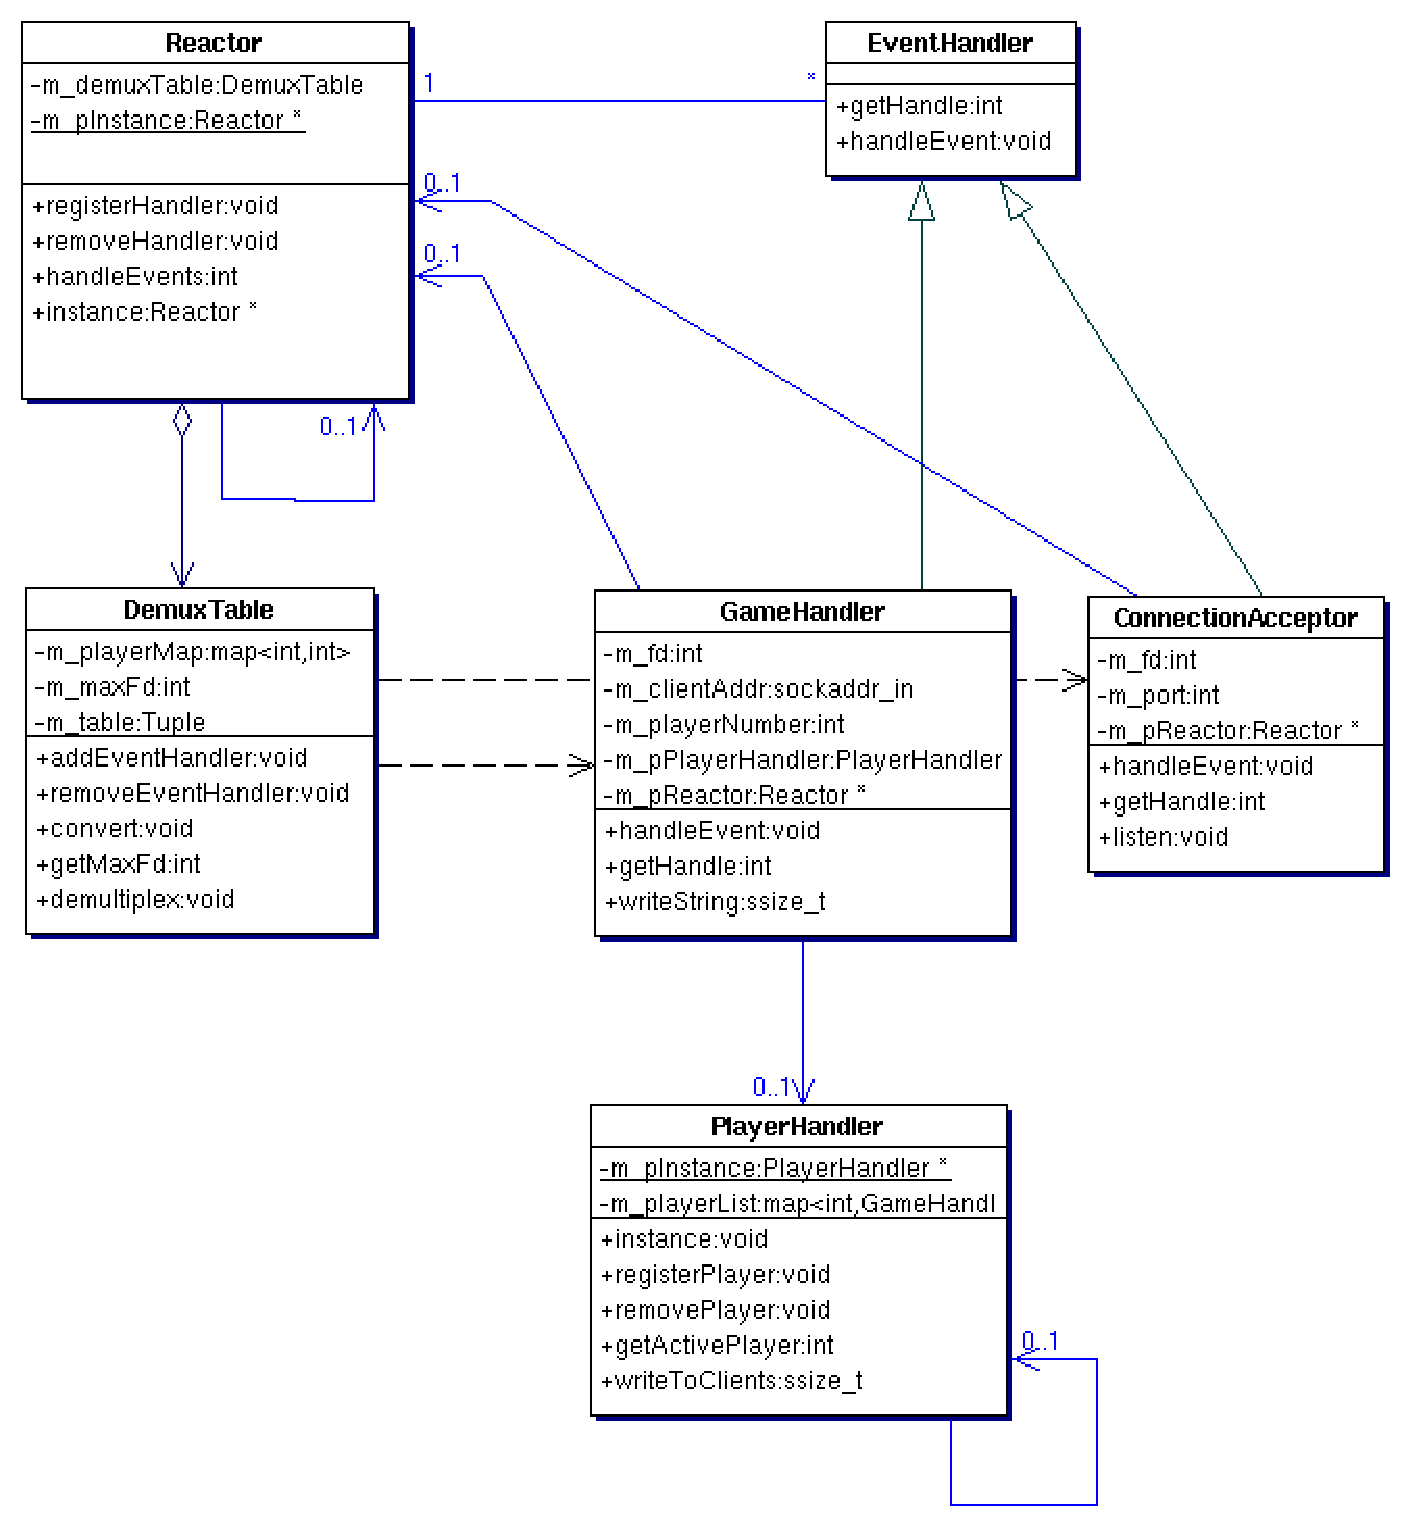
\includegraphics[width=12cm]{./images/reactor_klassendiagramm.pdf}}
  \end{center}
  \caption{Klassendiagramm Netzwerk/Server}
\end{figure}

\subsection{Beschreibung des Reactor Patterns}
Das Problem, dass sich bei einem Spiel, das erstens gewissen Geschwindigkeitsanforderungen gen"ugen muss und zweitens mehrere 
(mehr als 2) Mitspieler hat, ist, dass die Netzerwerkkommunikation speziell gel"ost werden muss, da alle Clients zu einem
nicht vorhersehbaren Zeitpunkt Meldungen zum Server schicken k"onnen. Da die Systemfunktionen, die f"ur die Kommunikation ben"otigt
werden (also read() und write() ) blockierend sind, muss entweder f"ur jeden Client ein seperater Prozess gestartet werden oder es 
muss ein geeignetes Pattern verwendet werden. Die erste L"osung w"are sehr einfach zu implementieren (wird auch sehr oft gemacht, zum
Beispiel bei Web Anwendungen), hat aber den Nachteil, dass bei einer Anwendung wie der unsrigen Interprozesskommunikation erforderlich
gewesen w"are, was sehr m"uhsam zu implementieren ist und auch Performance Nachteile mit sich bringt.
Die zweite L"osung mit dem Pattern erschien uns deshalb vorteilhafter, obwohl es auch nicht einfacher zu implementieren ist, 
aber die sinnvollere L"osung f"ur ein Spiel ist. 

Das Reactor Pattern hat folgende Vorteile
\begin{itemize}
	\item Wartezeiten und Antwortezeiten des Servers werden k"urzer da nicht blockierend auf einen Event eines einzigen Clients gewartet wird.
	\item Datendurchsatz wird erh"ort, da keine Daten zwischen einzelnen Prozessen ausgetauscht werden m"ussen.
	\item Sehr gute Wartungs- und Erweiterungseigenschaften, da "Anderungen nur an einem Ort gemacht werden m"ussen.
	\item Es ist kein Multithreading und keine Synchronisation im Server n"otig
\end{itemize}

Erreicht wird dies, indem synchron auf das Eintreffen von Ereignissen von verschiedenen Orten (Clients) gewartet wird. Diese Ereignisse
werden entgegengenommen, ausgewertet und an die bereitgestellten services weitergeleitet. Die Klassen und Methoden des Reactor 
Patterns werden in den folgenden Abschnitten erkl"art.
	
	
\subsection{Klasse Reactor (Singleton)}
Die Klasse ist daf"ur verantwortlich, die select() Funktion aufzurufen und anhand der Resultate, die sie von dieser Funktion erh"alt,
Reaktionen auszuf"uhren. Das heisst konkret, dass die select() Funktion, welche eine System Funktion ist, eine Meldung gibt, wenn ein 
Event eintrifft. Falls dies geschieht, ist die Reactor Klasse daf"ur verantwortlich, das richtige Handler Objekt (ConnectionAcceptor oder
GameHandler) aufzurufen. Damit stellt diese Klasse eine Abstraktion der select() Funktion dar und ist daf"ur verantwortlich, dass die
Handler Funktionen read() und connect() nur aufgerufen werden, wenn es tats"achlich n"otig ist. Damit wird gew"ahrleistet, dass
das System nicht blockiert, sondern dass alle Clients sehr schnell bedient und abgefragt werden k"onnen.
\subsubsection{Funktionen}
\begin{tabular}{p{50mm}p{90mm}}
	+registerHandler(EventHandler* pEventHandler, EventType eventType) : void  &  registriert einen neuen Event Handler (ConnectionAcceptor
	oder GameHandler) mit dem dazugeh"origen Event Typ in der Demultiplex Tabelle. \\
	+removeHandler(EventHandler* pEventHandler, EventType eventType)  : void  &  entfernt den Event Handler aus der Demultiplex Tabelle \\
	+handleEvents() : int     & f"uhrt die select() Funktion aus und ruft die 
	entsprechende Methode im ConnectionAcceptor bzw. im GameHandler auf. \\
	+instance() : Reactor* & gibt die Reactorinstanz zur"uck. \\ 
\end{tabular}


\subsection{Klasse EventHandler}
Diese Klasse ist eine rein virtuelle Klasse und stellt die Schnittstelle f"ur die abgeleiteten Klassen ConnectionAcceptor und GameHandler dar.

\subsection{Klasse ConnectionAcceptor}
Der ConnectionAcceptor ist daf"ur zust"andig, Verbindungsanfragen zu regeln. Das heisst, wenn sich ein Client mit dem Server verbinden m"ochte,
macht der ConnectionAcceptor eine neue Verbindung auf der Serverseite (erstellt einen neuen Filedeskriptor)
und falls es keine Fehler dabei gibt, wird ein neuer GameHandler erstellt.
\subsubsection{Funktionen}
\begin{tabular}{p{50mm}p{90mm}}
	+listen() : void & stellt einen Filedeskriptor mit der richtigen Struktur um Verbindungsanfragen entgegenzunehmen zur Verf"ugung und 
	registriert diesen beim Reactor. \\
	+handleEvent(int fd, EventType eventType) : void & ist eine "uberschriebene Funktion der Klasse EventHandler. Diese ist zust"andig, ankommende
	Anfragen f"ur eine Verbindung entgegenzunehmen und wenn kein Fehler auftritt, wird die Verbindung akzeptiert und ein neues GameHandler Objekt erstellt. \\
	+getHandle() : int & gibt den Filedeskriptor, der in der listen() Funktion bereitgestellt wurde zur"uck. \\
\end{tabular}

\subsection{Klasse GameHandler}
F"ur jeden Client, der sich verbunden hat, gibt es ein GameHandler Objekt. Dieses Objekt regelt die ganze Kommunikation zwischen Client und
Server f"ur diesen bestimmten Client. Das heisst, er nimmt alles, was vom Client zum Server geschickt wird entgegen und schreibt alles
vom Server zum Client. 
\subsubsection{Funktionen}
\begin{tabular}{p{50mm}p{90mm}}
	+handleEvent(int fd, EventType eventType) : void & ist eine "uberschriebene Funktion der Klasse EventHandler. Sie nimmt die
	Strings, die vom Client an den Server "ubermittelt wurden an und gibt diese an die PD weiter. \\
	+getHandle() : int & gibt den Filedeskriptor, der den GameHandler identifiziert zur"uck. \\
	+writeToClient(const char* str, size\_t n) : ssize\_t & Schreibt die Strings, die von der PD an die Clients "ubermittelt werden sollen zu dem
	Client, f"ur den das GameHandler Objekt zust"andig ist. \\
\end{tabular}

\subsection{Klasse DemuxTable}
Die Demultiplex Tabelle ist dazu da, die Filedeskriptoren mit ihren entsprechenden Eventtypen zu registrieren, 
damit bei einer Anfrage des Clients das richtige GameHandler Objekt
aufgerufen werden kann. Das heisst in dieser Tabelle sind alle File Deskriptoren mit den zugeh"origen Events gespeichert.
\subsubsection{Funktionen}
\begin{tabular}{p{50mm}p{90mm}}
	+convert(fd\_set\& read\_fds, fd\_set\& except\_fds) : void & konvertiert die Event-Typen um herauszufinden, was f"ur ein Event ansteht 
	(ein read oder connect Event)\\
	+addEventHandler(int fd, EventHandler* pEventHandler, EventType eventType) : void & ein EventHandler wird mit seinem Event Typ 
	in der Tabelle registriert.\\
	+removeEventHandler(int fd) : void & der EventHandler wird wieder aus der Tabelle entfernt.\\
	+getMaxFd() : int & der Zahlenwert des gr"ossten Filedeskriptors wird zur"uckgegeben.\\
	+demultiplex(int fdCount, fd\_set\& read\_fds, fd\_set\& except\_fds) : void & es wird anhand des Event-Typs in der Tabelle
	und des anstehenden Events herausgefunden, welche handleEvent() Funktion aufgerufen werden muss.\\
\end{tabular}

\section{Klasse PlayerHandler(Singleton)}
Im Netzwerk werden noch Assoziationen zwischen Filedeskriptor und Player (also Client) gemacht. Die PlayerHandler Klasse ist
von der Funktion her (nicht vom Aufbau) "ahnlich wie die Demultiplex Tabelle. Sie speichert f"ur jeden Client, also f"ur jeden GameHandler
einen Zeiger, damit sie diesen kennt. Wenn nun eine Meldung von der ServerPD an die Clients geschickt werden soll, wird in dieser Klasse
die entsprechende write() Funktion in allen GameHandler Objekten aufgerufen.
\subsubsection{Funktionen}
\begin{tabular}{p{50mm}p{90mm}}
	+registerPlayer(GameHandler* pGameHandler) : void & Wenn sich ein neuer Spieler angemeldet hat, wird hier das zugeh"orige GameHandler
	Objekt, das den Spieler identifiziert, registriert\\
	+removePlayer(GameHandler* pGameHandler) : void & Wenn die Verbindung zu einem Spieler nicht mehr besteht, wird der GameHandler dieses 
	Spielers hier entfernt.\\
	+getActivePlayer(GameHandler* pGameHandler) : int & gibt die Spielernummer (1-4) zur"uck. \\
	+instance() : WriteHandler* & die Instanz des PlayerHandler wird zur"uckgegeben. \\
\end{tabular}


\subsection{Client (Singleton)}
Die Client Klasse steuert die ganze Verbindung auf der Seite des Clients. Er macht die Verbindung zum Server, schickt daten an diesen und liest 
auch die Daten, die vom Server geschickt werden.
\subsubsection{Funktionen}
\begin{tabular}{p{50mm}p{90mm}}
	+makeConnection(const char* strPtr): int & er"offnet eine Verbindung zum Server mit der angegebenen IP\_Nummer und gibt den 
	Filedeskriptor, der diese Verbindung identifiziert zur"uck. \\
	+writeString(const char* str, size\_t n) : ssizt\_t & Schickt eine Meldung zum Server und gibt die L"ange der geschriebenen Zeichenkette
	zur"uck\\
	+readString() : ssize\_t & liest die Meldung vom Server und gibt die L"ange der Nachricht zur"uck. Die Funktion wird in einem
	eigenen Thread ausgef"uhrt, damit eine Meldung m"oglichst schnell entgegengenommen werden kann.\\
	+close() : void & schliesst die Verbindung zum Server \\
	+instance() : WriteHandler* & die Instanz des Clients wird zur"uckgegeben. \\
\end{tabular}


\section{Netzwerk Sequenzdiagramme}

\begin{figure}[H]
  \begin{center}
   \rotatebox{90}{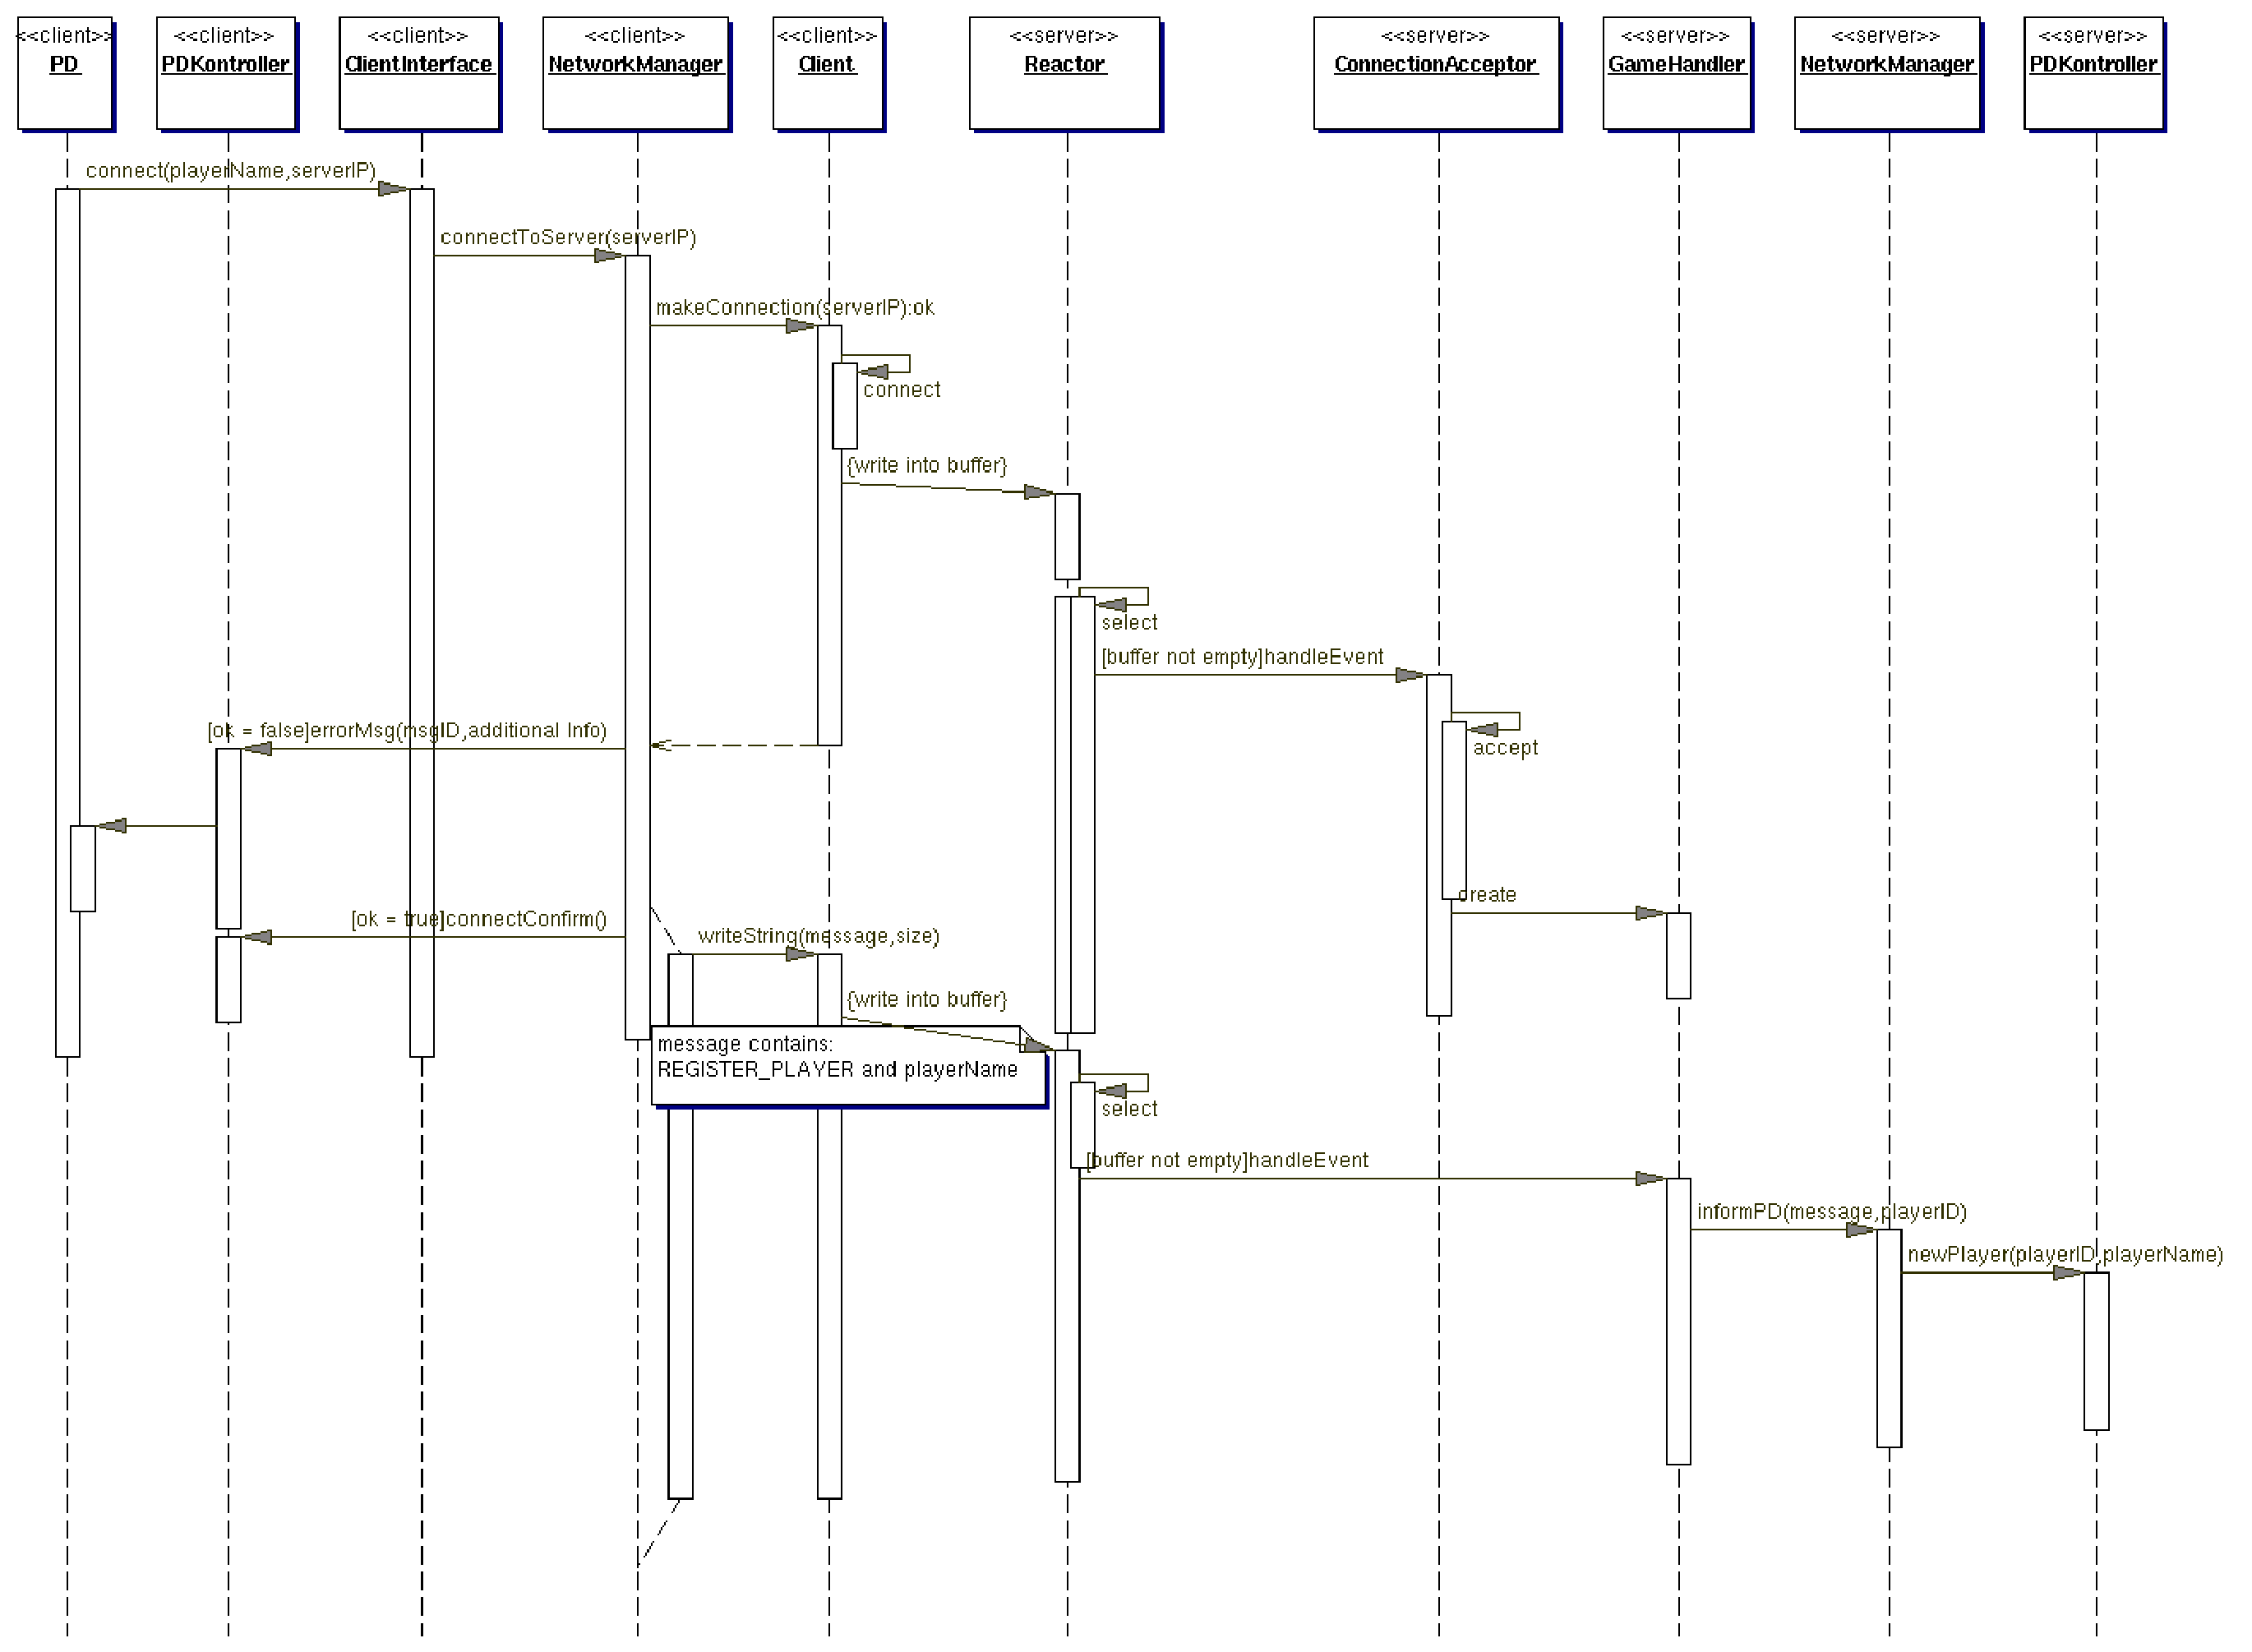
\includegraphics[width=18cm]{./images/clientconnect.pdf}}
  \end{center}
  \caption{Anmeldung des Clients bei einem Spiel}
\end{figure}

\begin{figure}[H]
  \begin{center}
    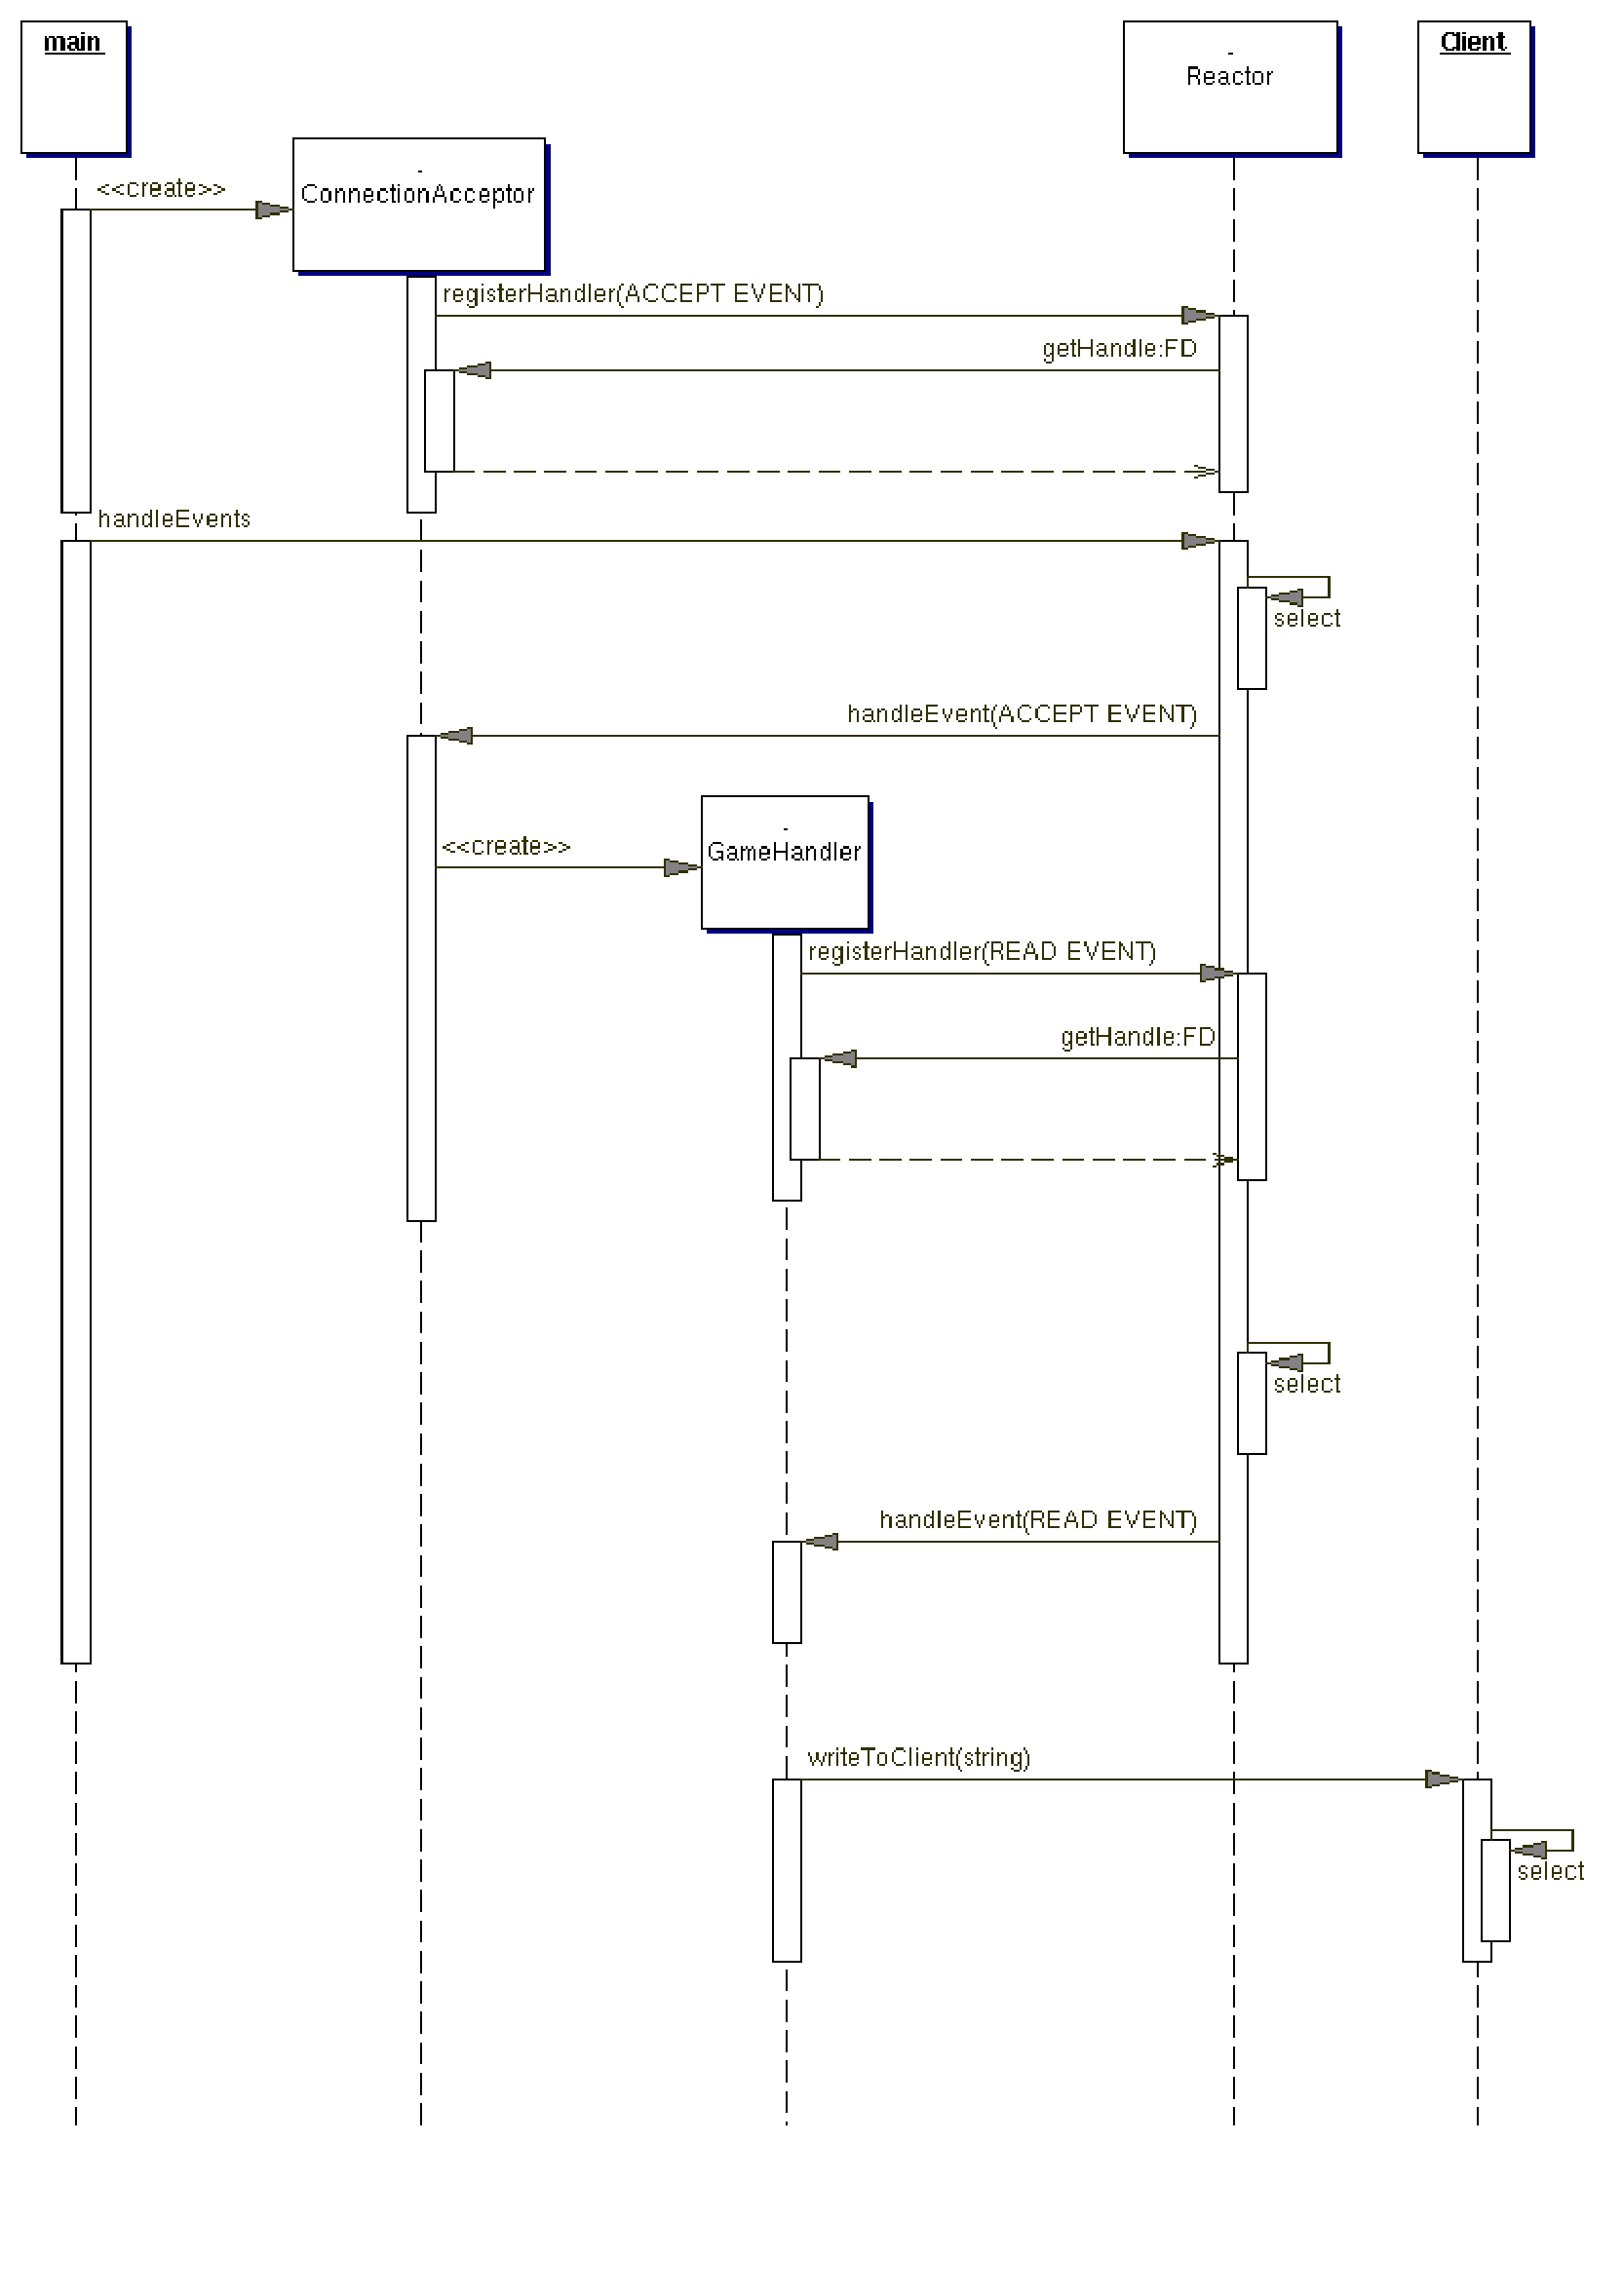
\includegraphics[width=12cm]{./images/sequenz_reactor.pdf}
  \end{center}
  \caption{Sequenzdiagramm Ablauf Server}
\end{figure}

\subsection{Erkl"arung Sequenzdiagramm Ablauf Server}
Im main Programm wird zuerst ein Objekt des ConnectionAcceptor erstellt. Dieser registriert sich anschliessend beim Reactor
und meldet damit, dass er f"ur ACCEPT EVENTS, das heisst f"ur ankommende Anfragen f"ur eine Verbindung, zust"andig ist.
Der Reactor registriert den ConnectionAcceptor in der Demultiplex Tabelle. Damit ist der erste Schritt gemacht und der Server
ist bereit, ankommende Verbindungsanfragen entgegenzunehmen.

Wenn das abgeschlossen ist, wird im Hauptprogramm (in einem eigenen Prozess) fortlaufend die Funktion handleEvents() des 
Reactors aufgerufen. Dieser f"uhrt den Systemaufruf select() durch, der pr"uft, ob eine Anfrage vorhanden ist. Ist dies der 
Fall, pr"uft er die Anfrage und im ersten Schritt wird das eine Verbindungsanfrage sein. Darauf ruft er handleEvent() im ConnectionAcceptor
auf, der die Anfrage entgegennimmt und bearbeitet. Falls es dabei keine Fehler gibt, wird ein neuer GameHandler erzeugt, der sich
gleich wieder beim Reactor registriert, diesmal aber f"ur READ EVENTS. Danach ist der Ablauf derselbe wie im ConnectionAcceptor.

Von nun an wird fortlaufend gepr"uft, ob eine Anfrage anliegt und wenn ja, wird der Typ der Anfrage ermittelt (READ oder ACCEPT Event) 
und die enstprechende Funktion im richtigen Objekt aufgerufen.

%end netzwerk design


%End Netzwerk Design


\part{Iteration 2}
% keine Vision notwendig f�r Iteration 2
% \chapter{Vision}

\section{Ausgangslage und Motivation}

Bomberman, ein unterhaltsames Spiel f"ur mehrere Spieler soll netztauglich und auf Linux portiert werden.
Bei herk"omlichen Windows-Versionen f"ur mehrere Spieler gestaltet sich
die gleichzeitig an einer Tastatur erfolgende Bedienung als "ausserst unkonfortabel. Ebenso stehen oft nicht
gleich drei weitere Mitspieler vor Ort zur Verf"ugung, darum soll eine Netzwerk taugliche Version geschaffen werden.
Das Spiel hat keine komplizierten Spielregeln.
Es soll mit einer ganzheitlich einfachen Handhabung realisiert werden, damit man unverz"uglich in
den Mehrspieler-Spielgenuss eintauchen kann.
\\
Da wir unser eigener Auftraggeber sind, begr"undet sich unsere Motivation auch in der Bew"altigung technologischer,
software-engineering orientierter und zwischenmenschlicher Aufgaben. Herausforderungen, die wir uns selber aufstellen.

\section{Features}

\subsection{Iteration 1}
\begin{itemize}{}{}
\item 1 Spielermodus
\item Spielfeld mit W"anden und Mauern
\item Spielfigur kann man bewegen
\item optional: Die Bewegungen des Spielers werden "ubers Netzwerk "ubertragen und auf einem anderen Rechner angezeigt
\end{itemize}

\subsection{Iteration 2}
\begin{itemize}{}{}
\item Es k"onnen Bomben gelegt werden, die explodieren
\item Spieler k"onnen sterben
\item Es k"onnen 4 Spieler zusammen "ubers Netzwerk spielen
\end{itemize}

\subsection{Optionen der Iteration 2}
\begin{itemize}
\item Es gibt Icons die der Spielfigur spezielle F"ahigkeiten verleihen
\item Soundeffekte sind zu h"oren
\item Hintergrundmusik ist zu h"oren
\item es gibt einen Pausemodus
\item eine Highscore der besten Spieler ist verf"ugbar
\end{itemize}

\section{Herausforderungen}

\subsection{Implementation}
\begin{itemize}{}{}
\item Animierte Grafik und Sound auf Linux
\item Netzwerk Implementation
\item Ablauf der Synchronisation des Spieles zwischen verschiedenen Rechnern
\end{itemize}

\subsection{Technologie}
\begin{itemize}{}{}
\item Linux
\item Dokumentation mit \LaTeX\
\item Design Software Together
\item Qt (Graphikbibliothek f"ur KDE Desktop)
\end{itemize}


\subsection{anderer Art}
\begin{itemize}{}{}
\item \textbf{{Zielgerichtetes Arbeiten}} \\
Durch die begrenzte, pro Woche zur Verf"ugung stehende Zeit(Ziel max. 4-8) und die vielseitige
 Aufgabenstellung, m"ussen wir zwangsl"aufig streng zielgerichtet arbeiten, um die Meilensteine
 erf"ullen zu k"onnen.

\item \textbf{{Teamwork (2"<Teamitglieder)}} \\
Ein Team mit mehr als zwei Personen erlaubt keine \textit{philosophischen}  Gruppendiskussionen mehr.
Es kann weder auf eine Traktandenliste f"ur Sitzungen, noch auf eine streng sachliche pro/contra
Argumentation w"ahrend einer Diskussion verzichtet werden.

\item \textbf{{Kompromissbereitschaft}} \\
Es muss von Perfektionismus zu notwendiger Zweckm"assigkeit hingearbeitet werden.

\item \textbf{{Eigeninitiative}} \\
Unser Team hat praktisch keine Erfahrungen aus gr"osseren Projekten mit gr"osseren Teams.
Gefragt sind Eigeninitiative zur Arbeit an eigener Teambereitschaft und Lernbereitschaft (nicht
nur f"ur Technologie sondern auch im Teambildungsprozess und Selbstorganisation).
\\
\textit{Anpacken ist angesagt, aber nicht blind ohne Priorisierung und Ziel sondern
        mit Blick zum Horziont und vereinten Kr"aften.
        }
\end{itemize}

\chapter{Anforderungsspezifikation}

\section{Einf"uhrung}

\subsection{Zweck}
Dieses Kapitel legt die Anforderungen an das Programm \textsc{NetBomb} fest.

\subsection{G"ultigkeitsbereich}
Semesterarbeit Software Engineering, Sommersemester 2002

\subsection{Definitionen, Akronyme, Abk"urzungen}
Siehe Anhang \ref{glossar} auf Seite \pageref{glossar}.

\section{Allgemeine Beschreibung}
\subsection{Spielregeln}

Ziel des Spiels ist es, die gegnerische Spielfigur mittels einer Bombe und dessen Bombenstrahl zu eliminieren.
Im Spiel gibt es zwei Spielfiguren, eine fixe Anzahl Mauern und eine variable Anzahl W"ande.
Die Spielfigur kann W"ande sprengen, Mauern sind unzerst"orbar.
Die Spielfigur kann weder durch W"ande noch durch Mauern gehen.
Unter gesprengten W"anden k"onnen sich Bomben oder Feuersymbole befinden. Das Aufheben einer Bombe erlaubt der Spielfigur
das Legen einer zus"atzlichen Bombe in Serie. Das Aufheben einer Flamme erlaubt der Spielfigur einen um ein Feld
l"angerer Bombenstrahl.
Die zwei Spielfiguren sind gegenseitig transparent. Sie k"onnen sich kreuzen.

\begin{figure}[H]
  \begin{center}
    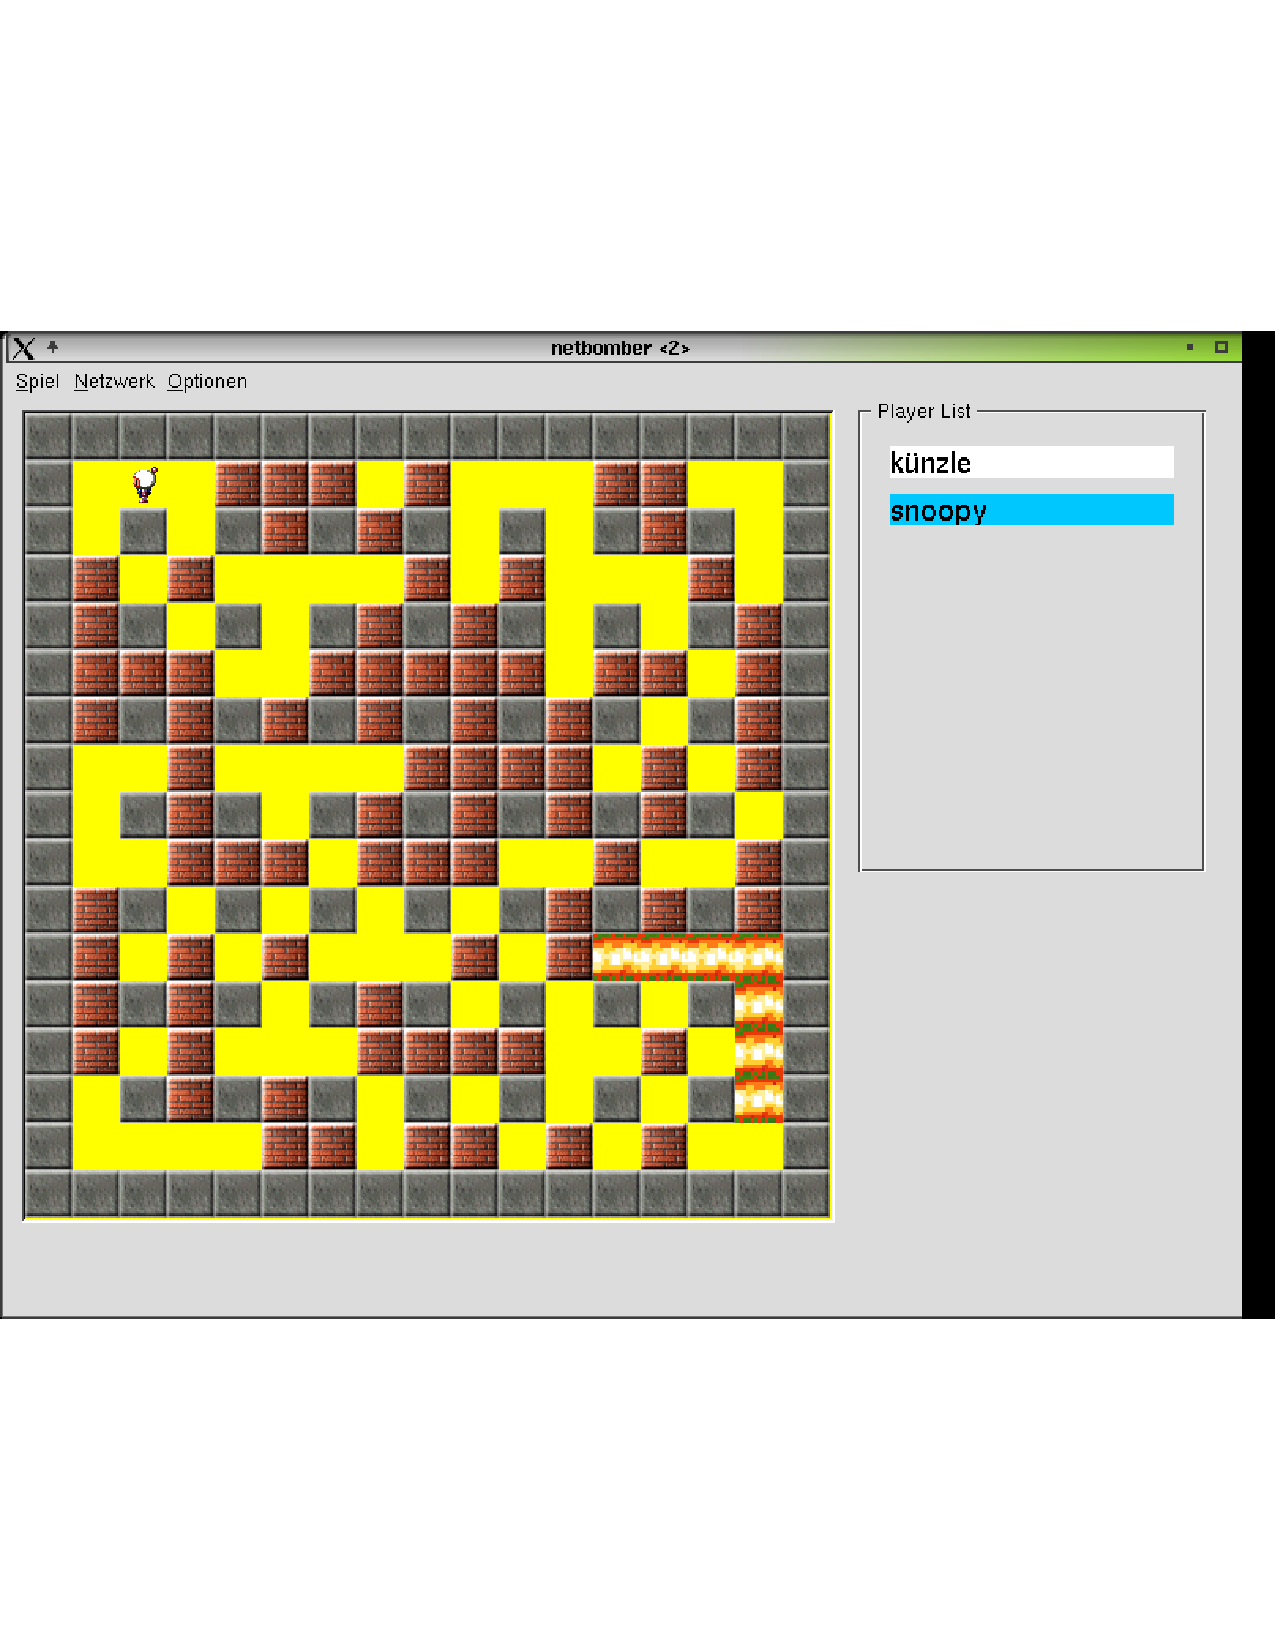
\includegraphics[width=10cm]{./images/spielfeld.pdf} \\
  \end{center}
  \caption{Bomberman Spiel}
\end{figure}

\subsection{Benutzergruppen}
Alle Menschen ob jung oder alt, weiblich oder m"annlich, die Freude an Computerspielen haben.

\subsection{M"ogliche Erweiterungen}
\begin{itemize}
\item Sound Unterst"utzung
\item spezielle Powerup-Icons, die von der Spielfigur aufgenommen werden k"onnen.
\item Highscore Anzeige
\end{itemize}

\subsection{Zu erwartende Probleme}
wurden bereits im Dokument Projektplan eingetragen.

\subsection{Annahmen}
Da die von uns verwendeten Technologien f"ur uns neu sind, sind wir uns bewusst, dass das Risiko vorhanden ist, dass wir
die Anforderungen nicht vollst"andig erf"ullen k"onnen. Dieses Dokument wurde in der Annahme geschrieben, dass wir die
auftretenden Probleme l"osen k"onnen. Ansonsten werden wir die Anforderungen zusammen mit dem Betreuer anpassen.

\subsection{Abh"angikeiten}
Funktionalit"at Qt-Bibliothek und KDE-Bibliothek.

\section{Anforderungen im Einzelnen}

\subsection{Funktionale Anforderungen Iteration 1}


\begin{table}[H]
  \begin{center}
    \begin{tabular}{|p{20mm}| p{85mm}| p{20mm}|}
    \multicolumn{3}{l}{\textbf{Spiel}} \\
    \hline Referenz & Funktion & Priorit"at \\
    \hline A1.1 & Spiel starten & 1 \\
    \hline A1.2 & Spiel beenden & 1 \\
    \hline A1.3 & Spielregeln "uberwachen & 1 \\
    \hline
    \end{tabular}
  \end{center}
  \caption{Spiel Funktionen Iteration 1}
\end{table}

\begin{table}[H]
  \begin{center}
    \begin{tabular}{|p{20mm}|p{85mm}|p{20mm}|}
    \multicolumn{3}{l}{\textbf{Spielfigur}} \\
    \hline Referenz & Funktion & Priorit"at \\
    \hline A2.1 & Figur bewegen & 1 \\
    \hline
    \end{tabular}
  \end{center}
  \caption{Spielfigur Funktionen Iteration 1}
\end{table}


\begin{table}[H]
  \begin{center}
    \begin{tabular}{|p{20mm}|p{85mm}|p{20mm}|}
    \multicolumn{3}{l}{\textbf{Spielfeld}} \\
    \hline Referenz & Funktion & Priorit"at \\
    \hline A3.1 & Hintergrund zeichnen & 1 \\
    \hline A3.2 & Mauern und W"ande zeichnen & 1 \\
    \hline A3.3 & Spielfigur zeichnen & 1 \\
    \hline
    \end{tabular}
  \end{center}
  \caption{Spielfeld Funktionen Iteration 1}
\end{table}


\subsection{Funktionale Anforderungen Ieration 2}


\begin{table}[H]
  \begin{center}
    \begin{tabular}{|p{20mm}|p{85mm}|p{20mm}|}
    \multicolumn{3}{l}{\textbf{Spiel}} \\
    \hline Referenz & Funktion & Priorit"at \\
    \hline A1.4 & Spielstand aktualisieren & 2 \\
    \hline A1.5 & Highscore speichern & 2 \\
    \hline
    \end{tabular}
  \end{center}
  \caption{Funktionen Spiel Iteration 2}
\end{table}



\begin{table}[H]
  \begin{center}
    \begin{tabular}{|p{20mm}|p{85mm}|p{20mm}|}
    \multicolumn{3}{l}{\textbf{Spielfigur}} \\
    \hline Referenz & Funktion & Priorit"at \\
    \hline A2.2 & Bombe legen  & 2 \\
    \hline A2.3 & sterben      & 2 \\
    \hline
    \end{tabular}
  \end{center}
  \caption{Funktionen Spielfigur Iteration 2}
\end{table}



\begin{table}[H]
  \begin{center}
    \begin{tabular}{|p{20mm}|p{85mm}|p{20mm}|}
    \multicolumn{3}{l}{\textbf{Spielfeld}} \\
    \hline Referenz & Funktion & Priorit"at \\
    \hline A3.4 & Wand entfernen & 2 \\
    \hline
    \end{tabular}
  \end{center}
  \caption{Funktionen Spielfeld Iteration 2}
\end{table}



\begin{table}[H]
  \begin{center}
    \begin{tabular}{|p{20mm}|p{85mm}|p{20mm}|}
    \multicolumn{3}{l}{\textbf{Bombe}} \\
    \hline Referenz & Funktion & Priorit"at \\
    \hline A4.1 & explodieren & 2 \\
    \hline A4.2 & Reichweite berechnen & 2 \\
    \hline
    \end{tabular}
  \end{center}
  \caption{Funktionen Bombe Iteration 2}
\end{table}



\begin{table}[H]
  \begin{center}
    \begin{tabular}{|p{20mm}|p{85mm}|p{20mm}|}
    \multicolumn{3}{l}{\textbf{Netzwerk}} \\
    \hline Referenz & Funktion & Priorit"at \\
    \hline A5.1 & Server starten & 2 \\
    \hline A5.2 & Client anmelden & 2 \\
    \hline A5.3 & Spielelement Position "ubermitteln & 2 \\
    \hline A5.4 & Spielsituation synchronisieren & 2 \\
    \hline
    \end{tabular}
  \end{center}
  \caption{Funktionen Netzwerk Iteration 2}
\end{table}

%Use Cases
\subsection{Use Cases Iteration 1}
\subsubsection{UC01 Spiel starten}

\begin{table}[H]
  \begin{center}
    \begin{tabular}{|p{40mm}|p{90mm}|}
    \hline Ausl"osender Aktor & Spieler  \\
    \hline Zweck / Ziel & Spielfeld und Spielelemente zeichnen, Netzwerkverbindung aufbauen  \\
    \hline Priorit"at & 1 \\
    \hline Style & casual \\
    \hline Anforderungen &  Iteration 1: A1.1, A1.2, A3.1, A3.2, A3.3 \\
		                     &  Iteration 2: inkl.A5.1, A5.2, A5.3, A5.4\\
    \hline Vorbedingung & - \\
    \hline Nachbedingung & Spielfeld und Spielelemente gezeichnet, Netzwerkverbindung aufgebaut. \\
    \hline Bemerkungen & - \\
    \hline
    \end{tabular}
  \end{center}
  \caption{UC01 Spiel starten}
\end{table}


\begin{center}
  \begin{tabular}{p{65mm} p{65mm}}
  \multicolumn{2}{l}{\textbf{Grundlegender Ablauf}} \\
  & \\
  \textbf{Aktor} & \textbf{System} \\
  1. Benutzer startet neues Spiel &  \\
  &  2. Leveldaten einlesen  \\
  &  3. Spielfeld zeichnen \\
  &  4. Spielelemente zeichnen \\
  &  5. wartet auf Benutzereingabe\\
  \multicolumn{2}{l}{\textbf{Erweiterungen}} \\
  \(\ast\)a zu jeder Zeit kann der Spieler das Spiel beenden & \\
  \end{tabular}
\end{center}


\subsubsection{UC02 Spielfigur bewegen}

\begin{table}[H]
  \begin{center}
    \begin{tabular}{|p{40mm}|p{90mm}|}
    \hline Ausl"osender Aktor & Spieler \\
    \hline Zweck / Ziel & Aktor kann Spielfigur in horizontaler oder vertikaler Richtung bewegen \\
    \hline Priorit"at & 1\\
    \hline Style & casual \\
    \hline Zu erf"ullende Anforderungen & A1.3, A2.1, A3.3 \\
    \hline Vorbedingungen & UC01 \\
    \hline Nachbedingungen & Die Spielfigur wurde um ein Feld verschoben.\\
    \hline Bemerkungen & Dieser UC kann 1 oder n mal ausgef"uhrt werden. \\
    \hline
    \end{tabular}
  \end{center}
  \caption{UC02 Spielfigur bewegen}
\end{table}


\begin{center}
  \begin{tabular}{p{65mm} p{65mm}}
  \multicolumn{2}{l}{\textbf{Grundlegender Ablauf}} \\
  & \\
  \textbf{Aktor} & \textbf{System} \\
  1. Der Aktor verschiebt die Spielfigur um ein Feld nach links, rechts, oben oder unten. & \\
  & 2. zeichnet die Figur auf dem neuen Feld, sofern das Zielfeld nicht einer Wand oder einer Mauer enstpricht. \\
  \end{tabular}
\end{center}

\subsection{Use Cases Iteration 2}
\subsubsection{UC03 Bombe legen}

\begin{table}[H]
  \begin{center}
    \begin{tabular}{|p{40mm}|p{90mm}|}
    \hline Ausl"osender Aktor & Spieler  \\
    \hline Zweck / Ziel & Der Spieler legt eine Bombe, die nach einer gewissen Zeit explodiert und
		                      alle vernichtbaren Objekte, die sich in Reichweite befinden zerst"ort\\
    \hline Priorit"at & 2 \\
    \hline Style & casual \\
    \hline Anforderungen &  A1.1, A1.3, A2.1, A2.2, A2.3, A3.1, A3.2, A3.3, A3.4, A4.1, A4.2\\
    \hline Vorbedingung & UC01 \\
    \hline Nachbedingung & Objekte die sich innerhalb der Reichweite befunden haben sind zerst"ort. \\
    \hline Bemerkungen & - \\
    \hline
    \end{tabular}
  \end{center}
  \caption{UC03 Bombe legen}
\end{table}


\begin{center}
  \begin{tabular}{p{65mm} p{65mm}}
  \multicolumn{2}{l}{\textbf{Grundlegender Ablauf}} \\
  & \\
  \textbf{Aktor} & \textbf{System} \\
  1. Der Spieler legt eine Bombe &  \\
	2. Der Spieler bewegt sich auf ein anderes Feld& \\
  &  3. Auf dem alten Feld wird eine Bombe dargestellt  \\
  &  4. Ein Timer startet \\
  &  5. Der Timer ist abgelaufen, auf allen Feldern (horizontal und vertikal zur Bombe) in Reichweite 
	wird eine Explosion dargestellt \\
  &  6. Zerst"orbare Elemente, die sich auf diesen Feldern befunden haben werden zerst"ort\\
  \multicolumn{2}{l}{\textbf{Erweiterungen}} \\
  \(\ast\)a zu jeder Zeit kann sich der Spieler auf benachbarte, begehbare Felder bewegen & \\
  \end{tabular}
\end{center}



\subsection{Optional}


\begin{table}[H]
  \begin{center}
    \begin{tabular}{|p{20mm}|p{85mm}|p{20mm}|}
    \multicolumn{3}{l}{\textbf{Spiel}} \\
    \hline Referenz & Funktion & Priorit"at \\
    \hline A1.6 & Spiel pausieren & 3 \\
    \hline A1.7 & Soundeffekte abspielen & 3 \\
    \hline A1.8 & Musik abspielen & 3 \\
    \hline
    \end{tabular}
  \end{center}
  \caption{optionale Funktionen Spiel}
\end{table}



\begin{table}[H]
  \begin{center}
    \begin{tabular}{|p{20mm}|p{85mm}|p{20mm}|}
    \multicolumn{3}{l}{\textbf{Spielfigur}} \\
    \hline Referenz & Funktion & Priorit"at \\
    \hline A2.4 & Bombe-Powerup aufnehmen & 3 \\
    \hline A2.5 & Flamme-Powerup aufnehmen & 3 \\
    \hline
    \end{tabular}
  \end{center}
  \caption{optionale Funktionen Spielfigur}
\end{table}


\begin{table}[H]
  \begin{center}
    \begin{tabular}{|p{20mm}|p{85mm}|p{20mm}|}
    \multicolumn{3}{l}{\textbf{Spieloptionen}} \\
    \hline Referenz & Funktion & Priorit"at \\
    \hline A6.1 & Sound ein/aus & 3 \\
    \hline A6.2 & Highscores anzeigen & 3 \\
    \hline A6.3 & Spielername eingeben & 3 \\
    \hline
    \end{tabular}
  \end{center}
  \caption{Spieloptionen}
\end{table}


\subsection{Leistungs- und Mengenanforderungen}
\label{LeistungsAnforderungen2}
\subsubsection{Leistungsanforderungen}
Um die Spielbarkeit "ubers Netzwerk zu gew"ahrleisten, muss der Spielstatus von allen Spielern mindestens
alle 150ms synchronisiert werden.

\subsubsection{Mengenanforderungen}
Keine.

\subsection{Anforderungen an Schnittstellen}

\subsubsection{Benutzerschnittstelle}
Das System ist mit dem Keyboard und der Maus bedienbar.

\subsubsection{Software Schnittstellen}
Qt, KDE-Library

\subsection{Randbedingungen f"ur den Entwurf}

\subsubsection{"Ubereinstimmungen mit Normen}
SE01/02

\subsubsection{Einschr"ankungen bez"uglich Software}
Lauff"ahig unter KDE 2.2 mit Qt 2.3.1

\subsubsection{Einschr"ankungen bez"uglich Hardware}
Lauff"ahig unter allen UNIX-Derivaten, die KDE unterst"utzen. Die Leistungsanforderungen gelten f"ur ein Netzwerk (mind. 10Mb/s)
ohne zus"atzlichen Datenverkehr.

\subsection{Merkmale}

\subsubsection{Benutzbarkeit}
Die Bedienung des Programms entspricht den g"angigen KDE-Programmen:\\
\href{http://developer.kde.org/documentation/standards/kde/style/basics/index.html}{http://developer.kde.org/documentation/standards/kde/style/basics/index.html}

\subsection{Andere Anforderungen}

\subsubsection{Inbetriebnahme / Installation}
Standardinstallationsweg eines Linux-Quellcodes (configure, make, make install)
In der Datei README finden Sie bez"uglich Inbetriebnahme detaillierte Informationen.

\subsubsection{Konfigurierbarkeit}
Alle Konfigurationen werden gespeichert. Die IP-Adresse des Spielservers kann eingegeben werden.
Optional kann der Spielername eingegeben werden.






\chapter{Supplementary Specification}

\section{Functionality}

\subsection{Error handling}
Fehler werden dem Spieler mittels einer Fehlermeldung gemeldet.
Die Fehler werden nicht persistent in einer log-datei gespeichert.

\subsection{Security}
Das Programm hat keine speziellen Sicherheitsvorkehrungen. Es kommuniziert "uber ein IP-Netz mit den Programmen der anderen Spieler.

\section{Performance}
Mit den unter \ref{LeistungsAnforderungen} auf Seite \pageref{LeistungsAnforderungen} angegebenen Leistungsanforderungen soll ein angenehmes Spielverhalten gew"ahrleistet werden.
\section{Supportability}

\section{Free open source components}
Als Linux-Software-Developers liegt es Nahe, OpenSource Technologien zu verwenden.
(siehe dazu Projektplan, Kapitel Technologien)

\section{Developer Guidelines}

\subsection{Code Guidelines}

\begin{itemize}
  \item Methodennamen beginnen mit Kleinbuchstaben
  \item Klassennamen beginnen mit Grossbuchstaben
  \item Variabeln beginnen mit Kleinbuchstaben
  \item Vor und nach Operations-Zeichen wird ein Abstand gemacht.
  \item Nach zusammengeh"origen Code-Bl"ocken eine leere Zeile einf"ugen.
  \item Bei Klassen die "offnende geschweifte Klammer rechts neben dem Klassennamen und die schliessende auf eine eigene Zeile.
        F"ur alle anderen F"alle die "offnende und schliessende geschweifte Klammer auf eine eigene Zeile.
  \item Code innerhalb geschweifter Klammern wird einger"uckt.
  \item Falls Tabulatoren verwendet werden, in der Entwicklungsumgebung definieren, dass daf"ur Leerzeichen eingef"ugt werden.
  \item Default-Einr"uckung: Zwei Leerzeichen
  \item jede Kommentarzeile mit zwei slashes (//) beginnen.
\end{itemize}

\subsection{GUI Guidelines}
Folgt sp"ater in einem speraten Dokument.

\chapter{Domainanalyse}

\section{Konzeptionelles Modell}

\begin{figure}[H]
  \begin{center}
    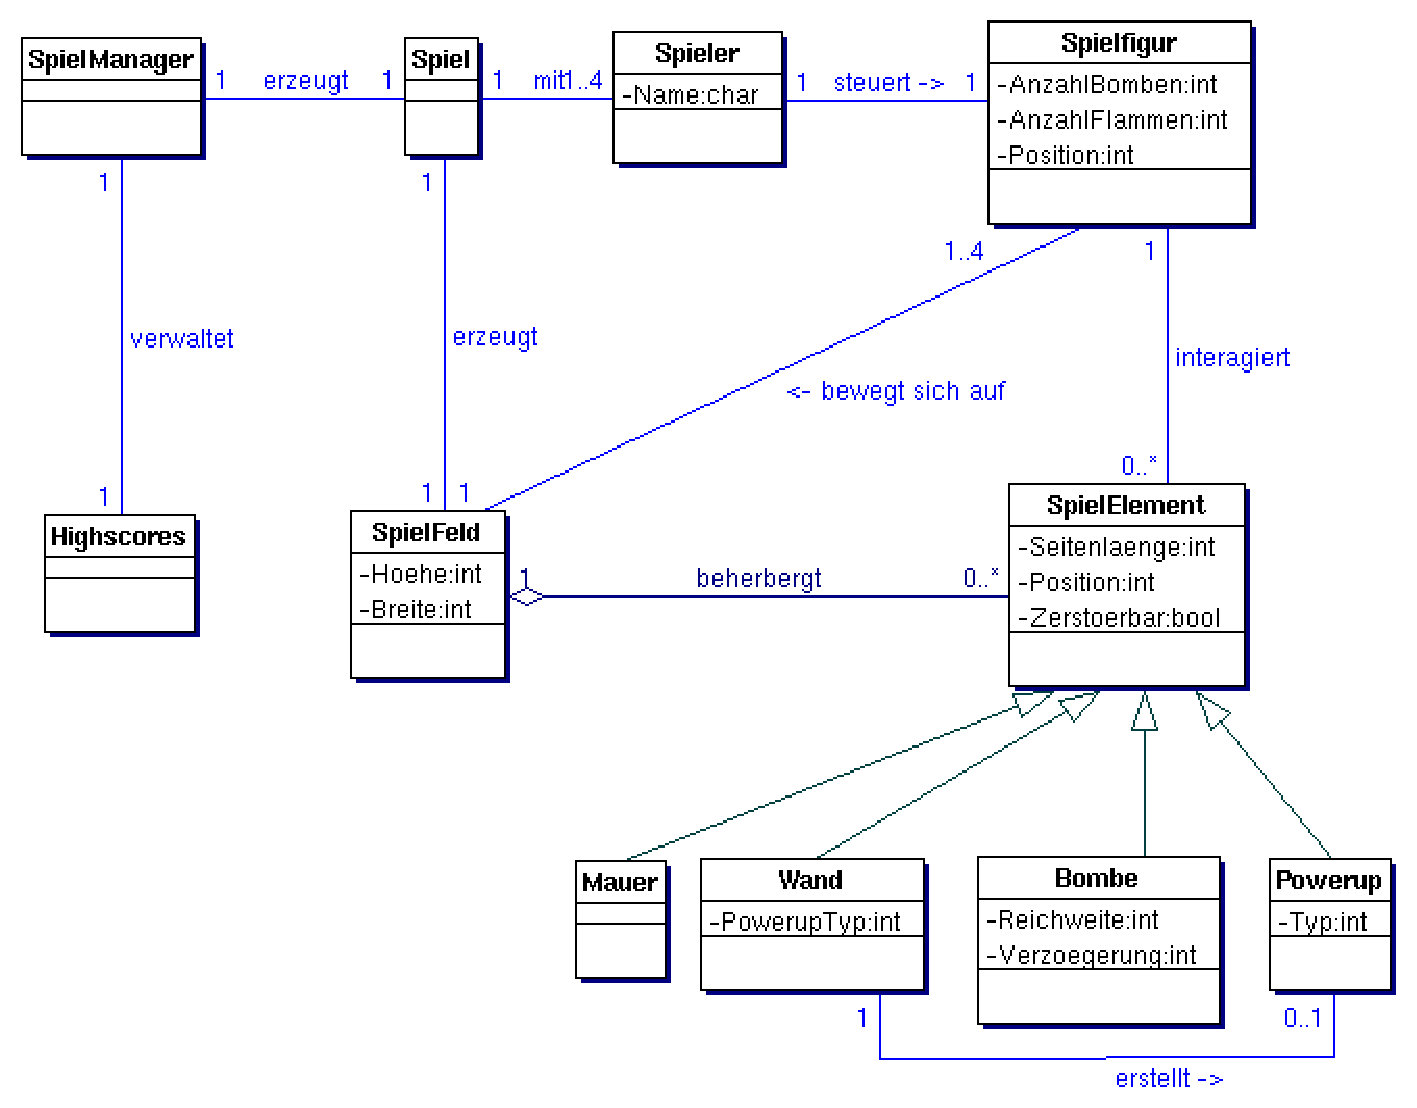
\includegraphics[width=14cm]{./images/domainmodell.pdf}
  \end{center}
  \caption{Domainmodell}
\end{figure}

\subsection{Spielmanager}
Der SpielManager ist f"ur die Initialisierung des Spiels zust�ndig. Er kennt die zwei Spieler und weitere f"ur das Spiel
notwendige Parameter.

\subsection{Spiel}
Das Spiel erzeugt das Spielfeld und positioniert die Spielelemente f"ur den Start des Spiels.

\subsection{Spielfeld}
Das Spielfeld ist der Hintergrund auf dem das eigentliche Spiel stattfindet. Es hat eine bestimmte H"ohe und Breite die zu beginn
festgelegt werden. Auf dem Spielfeld befinden sich die Objekte des Spielfeldes:Spielelemente und Spielfigur. Alle Objekte
des Spielfeldes haben eine Position. Das Spielfeld kennt alle Objekte und ihre Positionen.

\subsection{Spielelement}
Das Spielelement dient als Oberklasse f"ur s"amtliche sich auf dem Spielfeld befindlichen Objekte, ausser der Spielfigur.
Die einheitliche Schnittstelle erleichtert die Realisierung einiger Funktionen wie die Zerst"orung von Objekten usw.
Ein Objekt des Spielfeldes belegt normalerweise ein Feld auf dem Spielfeld.
Es kann "uber das Spielfeld die Belegung der benachbarten Felder abfragen.

\subsection{Spielfigur}
Die Spielfigur ist das einzige Objekt des Spielfeldes das sich auf dem Spielfeld bewegen kann. Sie kann mit den Spielelementen
kommunizieren. Die Spielfigur kann zum Beispiel Bomben erzeugen (legen) oder Powerups aufnehmen. Andererseits wird sie
von Mauern und W"anden am weitergehen gehindert.

\subsection{Mauer}
Die Mauer wird vor Spielbeginn erzeugt und bleibt w"ahrend dem ganzen Spiel an ihrem Platz. Sie kann nicht zerst"ort werden, trotzt
also auch explodierenden Bomben.

\subsection{Wand}
Die Wand wird ebenfalls zu beginn erzeugt, kann aber durch Bomben gesprengt werden und verschwindet in diesem Fall vom Spielfeld.
Eine Wand kann (muss aber nicht) ein Powerup beherbergen. Dieses bleibt auf dem Feld liegen falls die Wand zerst"ort wird.

\subsection{Bombe}
Die Bombe wird von der Spielfigur erzeugt. Dabei werden die Attribute wie Reichweite und Verz"ogerungszeit gesetzt. Danach ist
die Bombe ein eigenst"andiges Spielelement und explodiert entweder nach Ablauf der Verz"ogerungszeit oder wenn sie von einer
anderen Bombe gesprengt wird. Nach dem Explodieren meldet sie ihr Ableben der Spielfigur, die sie erzeugt hat.

\subsection{Powerup}
Ein Powerup ist entweder vom Typ Bombe (eine Bombe mehr in serie) oder vom Typ Flamme (gr"ossere Reichweit) und ist zu Beginn
unter einer Wand verborgen. Es tritt erst in erscheinung wenn die Wand durch eine Bombe zerst"ort wurde.
Betritt eine Spielfigur dasselbe Feld, nimmt sie das Powerup auf und es wird gel"oscht. Wird das Powerup von einer explodierenden
Bombe erfasst, wird es zerst"ort.

\subsection{Spieler}
Der Spieler hat einen Namen und steuert die Spielfigur. Er kann sie in alle 4 Richtungen bewegen und Bomben legen.

\chapter{Software Architektur}

\section{Logische Sicht}
Das System besteht aus prim"ar 4 Schichten (3  Schichten - Architektur plus Netzwerk). Diese beinhalten:
\begin{description}
\item[Schicht 1] Graphisches User Interface (GUI)
\item[Schicht 2] Problem Domain (PD)
\item[Schicht 3] Datenhaltung (DH)
\item[Schicht 4] Netzwerk (bestehend aus Client und Server)
\end{description}

\begin{figure}[H]
  \begin{center}
    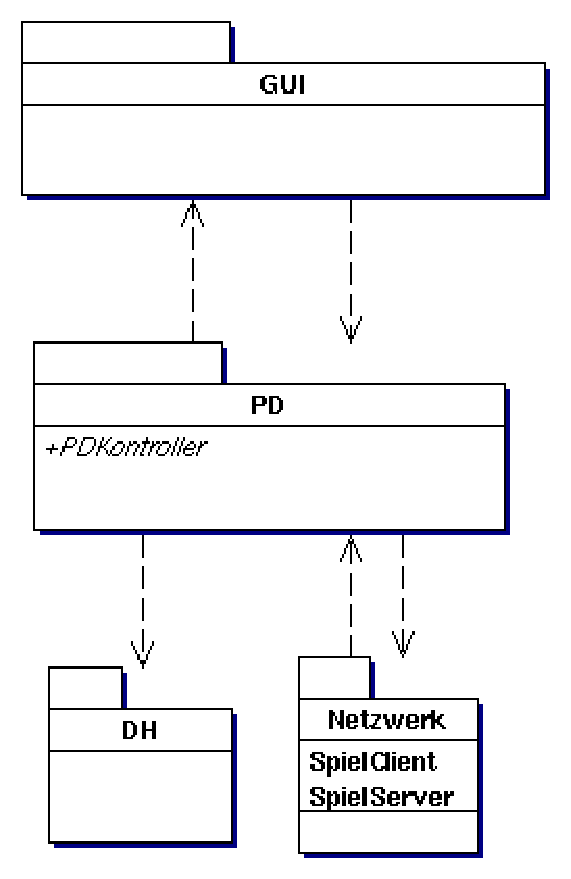
\includegraphics[height=8cm]{./images/architektur.pdf}
  \end{center}
  \caption{Schichtenmodell}
\end{figure}

Diese Architektur haben wir gew"ahlt um eine klare Trennung zwischen den einzelnen Programmteilen zu erreichen. \\
Das graphische User Interface ist die Schnittstelle zum Benutzer. "Uber dieses kann er Eingaben machen oder in unserem Fall erfolgt die Steuerung
der Spielfigur "uber das GUI. \\
Die PD ist die Schicht zwischen GUI und DH. Das heisst sie bekommt und verarbeitet Befehle vom GUI, schreibt Daten in die DH und
ruft Funktionen in der Netzwerkschicht auf. \\
Die Datenhaltung ist daf"ur zust"andig, Daten, die konsistent sein m"ussen zu speichern, damit sie bei einem Neustarten des Spiels wieder
zur Verf"ugung stehen. \\
Die Netzwerkschicht regelt die Daten"ubertragung zwischen dem Server und den Clients.



\section{Netzwerk}

\begin{figure}[hp]
  \begin{center}
    {\rotatebox{90}{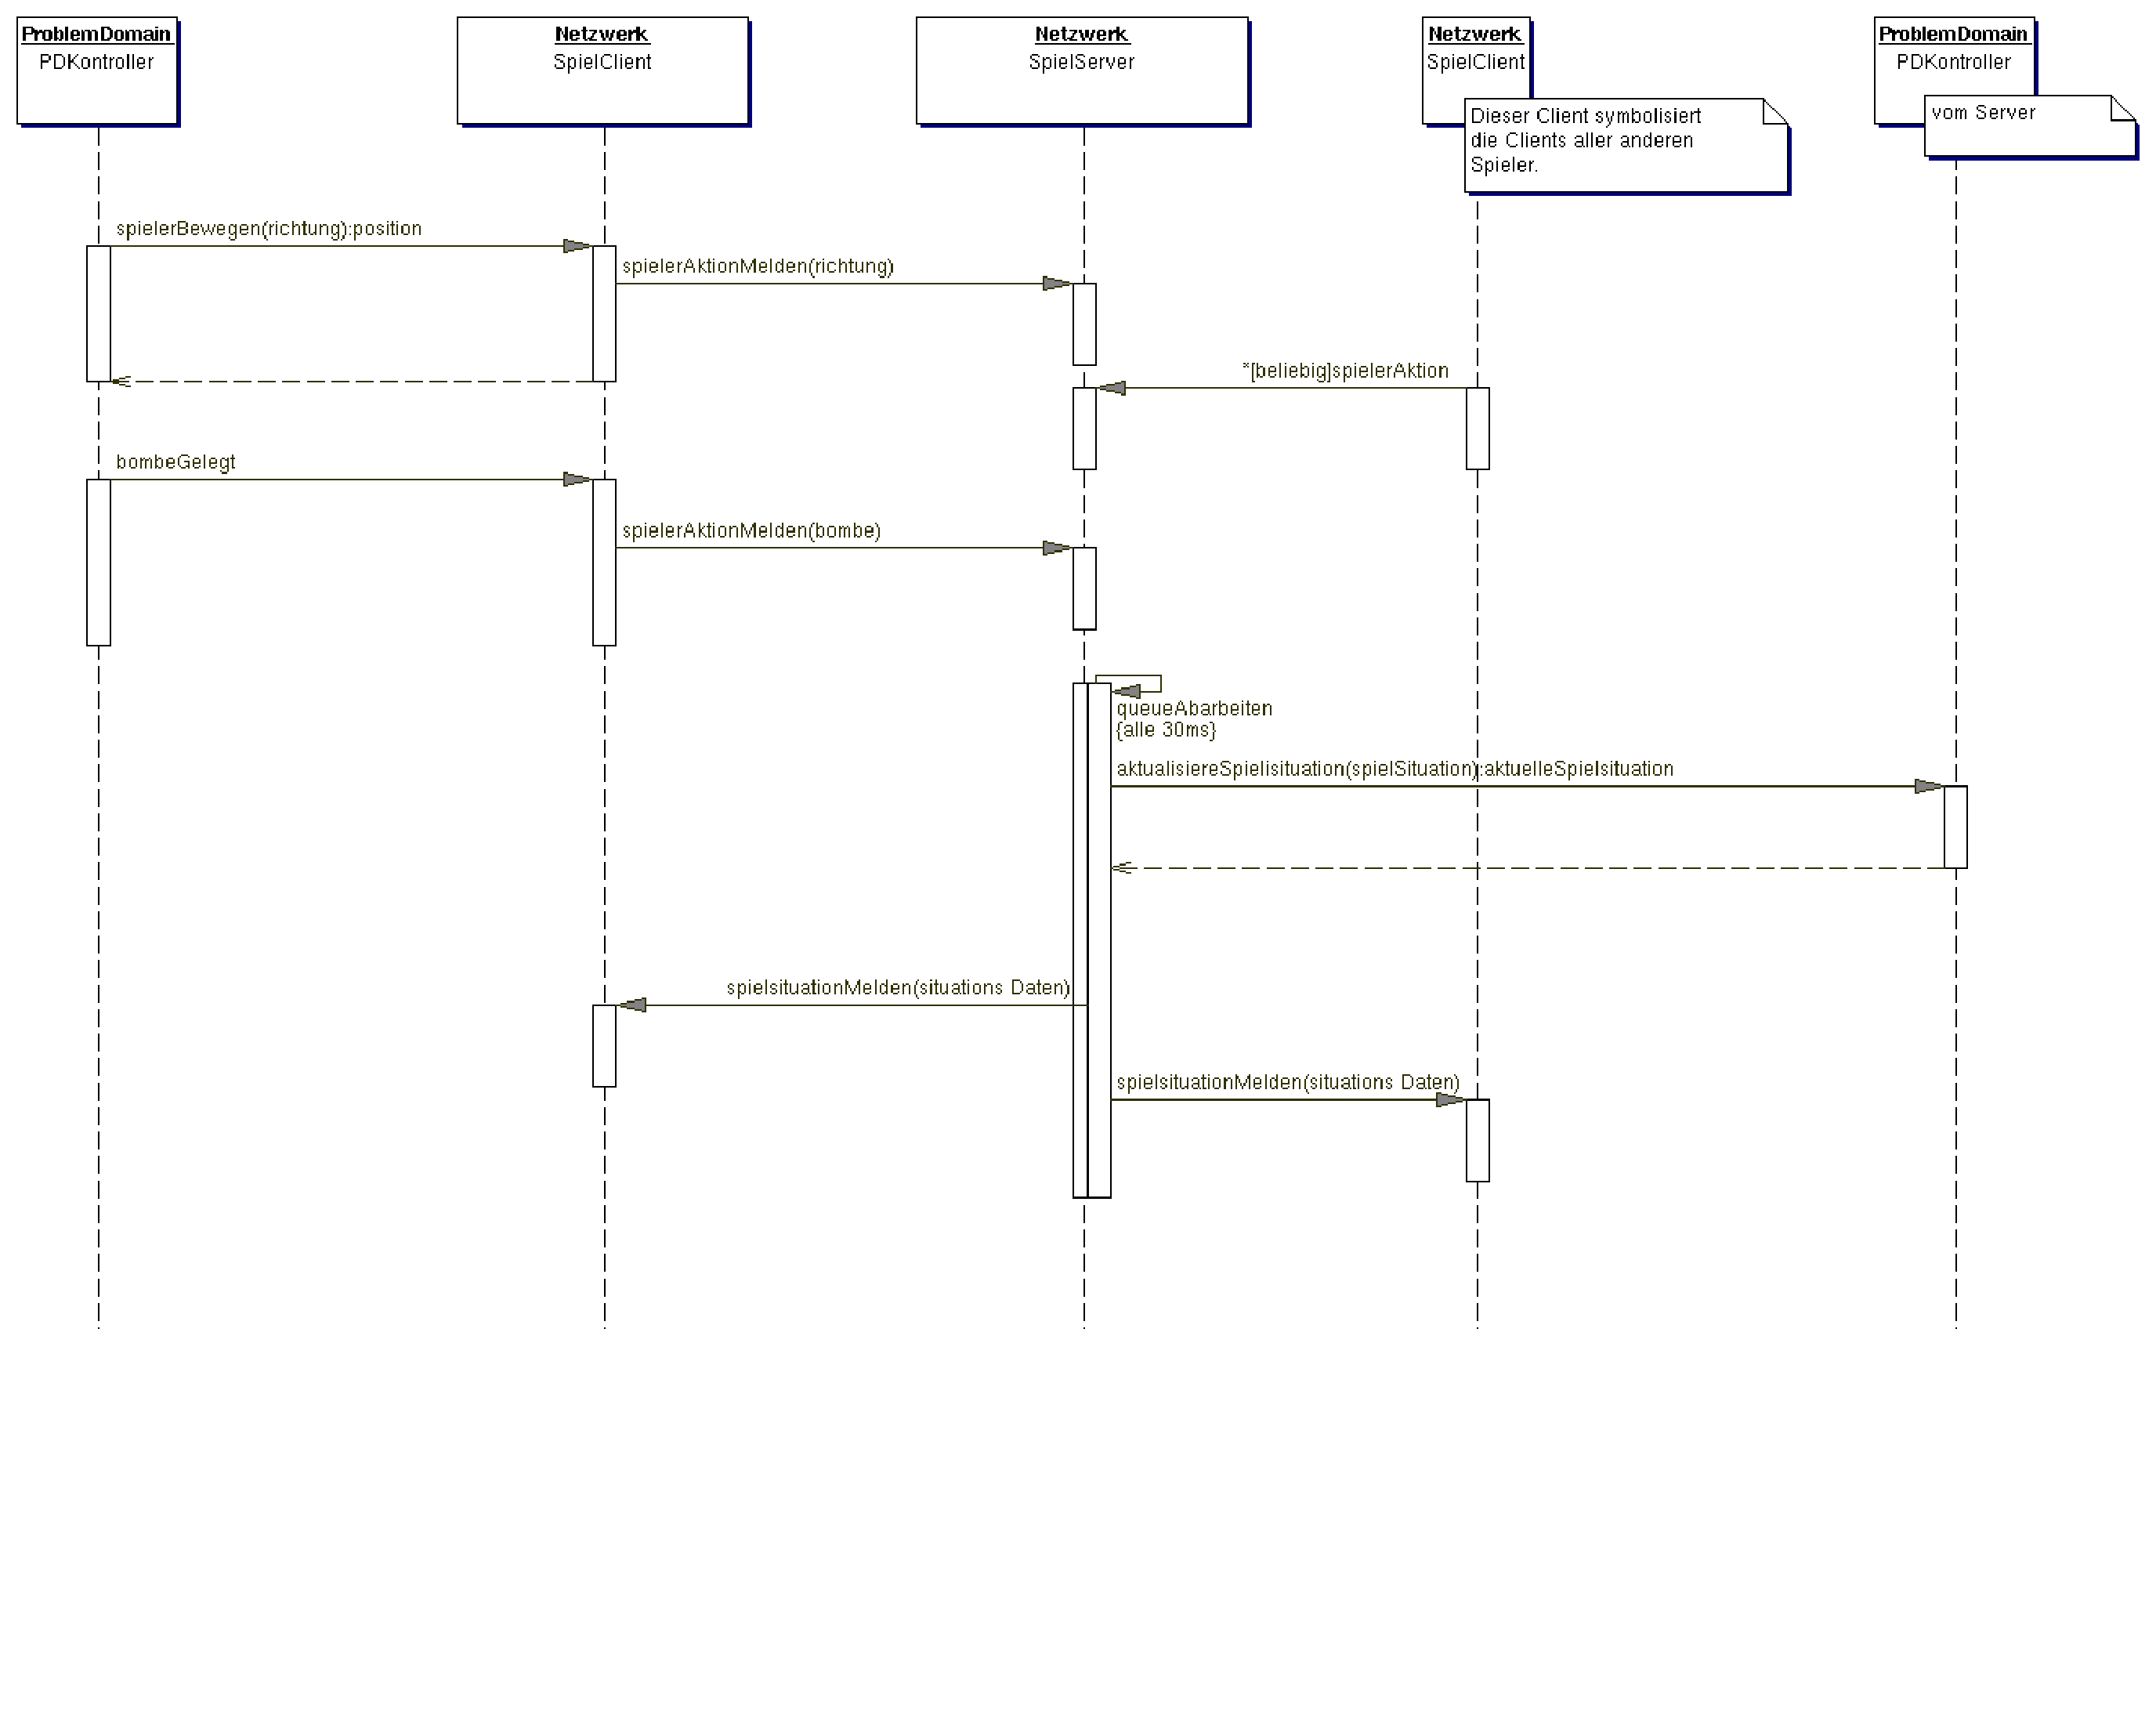
\includegraphics[height=16cm]{./images/netzwerk_aktion.pdf}}}
  \end{center}
  \caption{Interaktionsmodell Netzwerk}
\end{figure}

Das Netzwerk besteht aus einem Server und bis zu vier Clients die miteinander kommunizieren. Dabei kann jeder Client auch Server sein, das heisst
zu Beginn des Spiels entscheidet der Spieler, ob er Server und Client oder nur Client ist. Es kann nur ein Spieler Server sein.
Ist ein Spieler Server und Client, werden die Daten der Mitspieler zu ihm "ubermittelt. Das geschieht folgendermassen: \\
Die aktuellen Bewegungen eines Clients, also eines Spielers, werden zum Server "ubermittelt. Diese Daten werden vom Server
entgegengenommen. Dieser berechnet damit die aktuelle Position und allf"allige Aktionen des Clients. Diese berechnete Postion schickt der Server dann \textit{allen} Clients
zur"uck. Das heisst, jeder Client bekommt vom Server einen Snapshot. Zus"atzlich zur Position beinhaltet dieser wichtige Daten wie zum Beispiel ob
eine Bombe gelegt worden ist oder ein Powerup aufgenommen wurde. Mit diesen Angaben berechnet der Client selbst"andig, was auf dem
Spielfeld passiert. Er macht also dieselben Berechnungen wie der Server. Falls ein Spielelement gel"oscht werden muss,
versucht der Client das zu machen. Da er aber nicht selbst"andig Elemente l"oschen darf, wartet er auf den Befehl des Servers,
das entsprechende Element zu l"oschen. Der Client f"uhrt also nur eine Art Dummy-Funktion aus.
Damit erreichen wir eine bessere Performace wie mit dem Prinzip, bei dem alle Daten vom Server zum Client geschickt werden und zudem
k"onnen wir damit sicherstellen, dass alle Clients den selben Spielstand haben. Die Verbindung l"auft "uber TCP, was das Ankommen
der Pakete sicherstellt. \\
Der Server wurde mit dem Reactor Pattern implementiert. Dieses wird nachfolgend noch genauer erkl"art.

\chapter{Designmodell}

%begin pd design
\section{GUI Externes Design}

\begin{figure}[H]
  \begin{center}
    {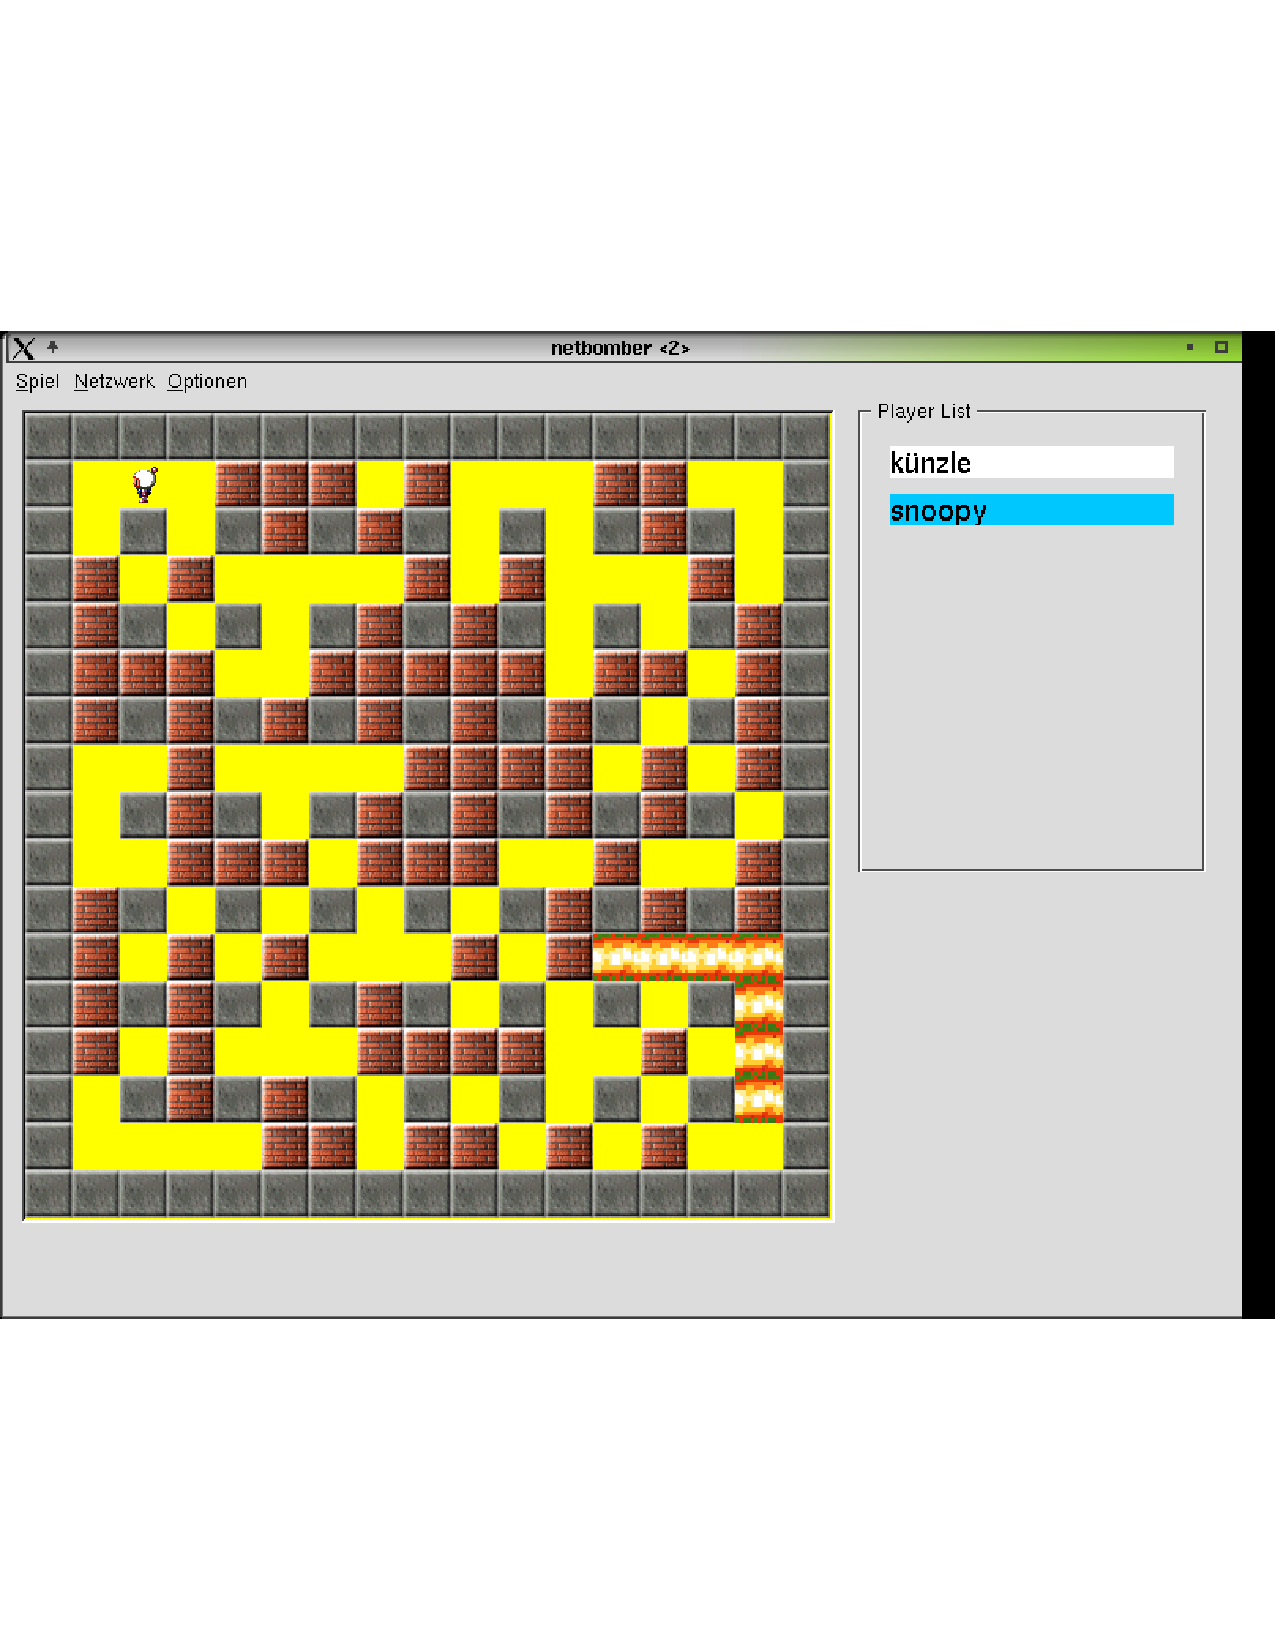
\includegraphics[height=12cm]{./images/spielfeld.pdf}}
  \end{center}
  \caption{Endversion des GUIs}
\end{figure}
Das Spielfeld (links) besteht aus diversen Spielelementen.
Diese werden dynamisch geladen, je nach dem was der Server
verlangt zum Darstellen. Rechts vom Spielfeld befindet sich
die Playerlist. Jeder Spielername wurde unterschiedlich
eingef"arbt, genau so wie die Farbe des entsprechenden Kopfes
der Spielfigur.

Die Farben der Spielfiguren:
\begin{table}[H]
	\begin{center}
		\begin{tabular}{|p{50mm}|p{30mm}|p{60mm}|}
		\hline Spielfigur 1 & Weiss & RGB (255, 255, 255) \\
		\hline Spielfigur 2 & Blau  & RGB (0, 200, 255) \\
		\hline Spielfigur 3 & Gr"un  & RGB (60, 255, 0) \\
		\hline Spielfigur 4 & Violet & RGB (255, 60, 255) \\
		\hline 
	\end{tabular}
	\end{center}
	\caption{Farben der Spielfiguren}
\end{table}


\begin{figure}[H]
  \begin{center}
    {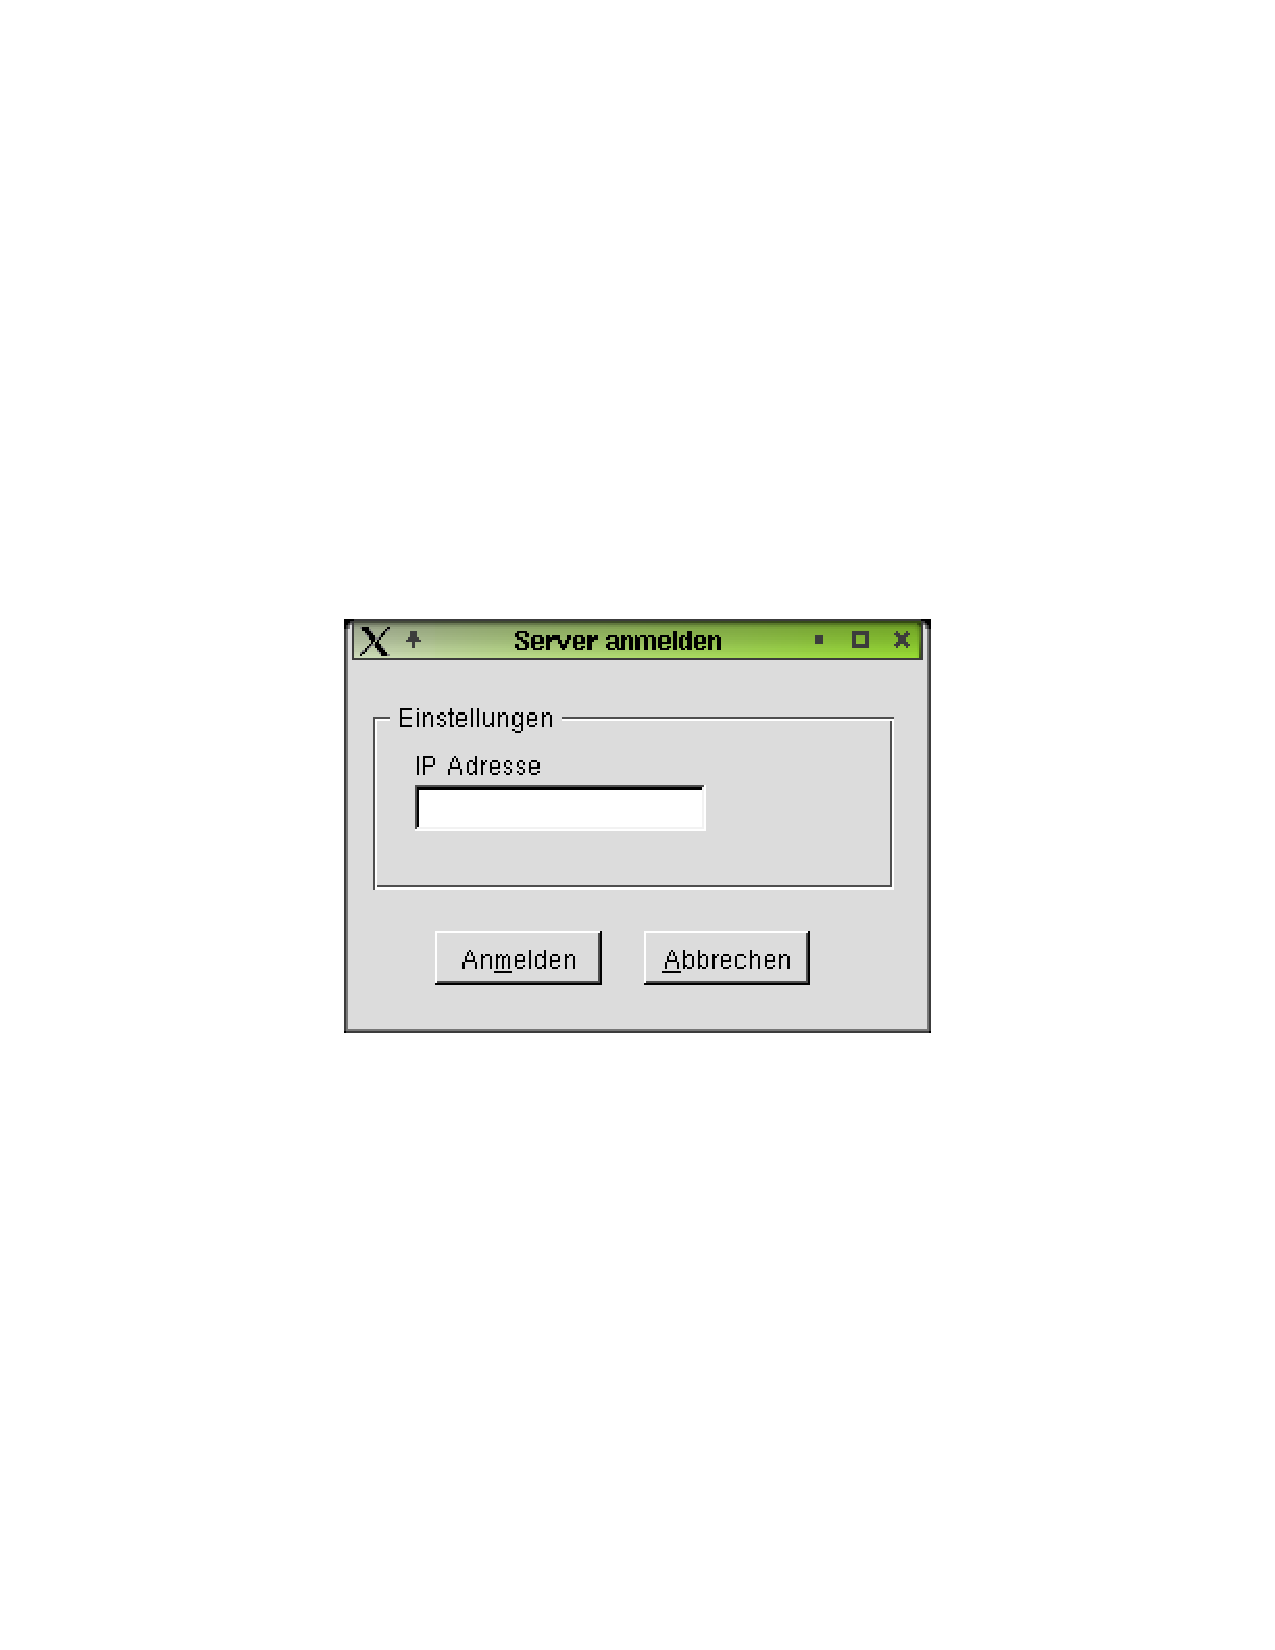
\includegraphics[height=6cm]{./images/joinserver.pdf}}
  \end{center}
  \caption{Snapshot des Dialoges Server anmelden}
\end{figure}

Dieser Dialog dient zum Anmelden an einen Server.

\begin{figure}[H]
  \begin{center}
    {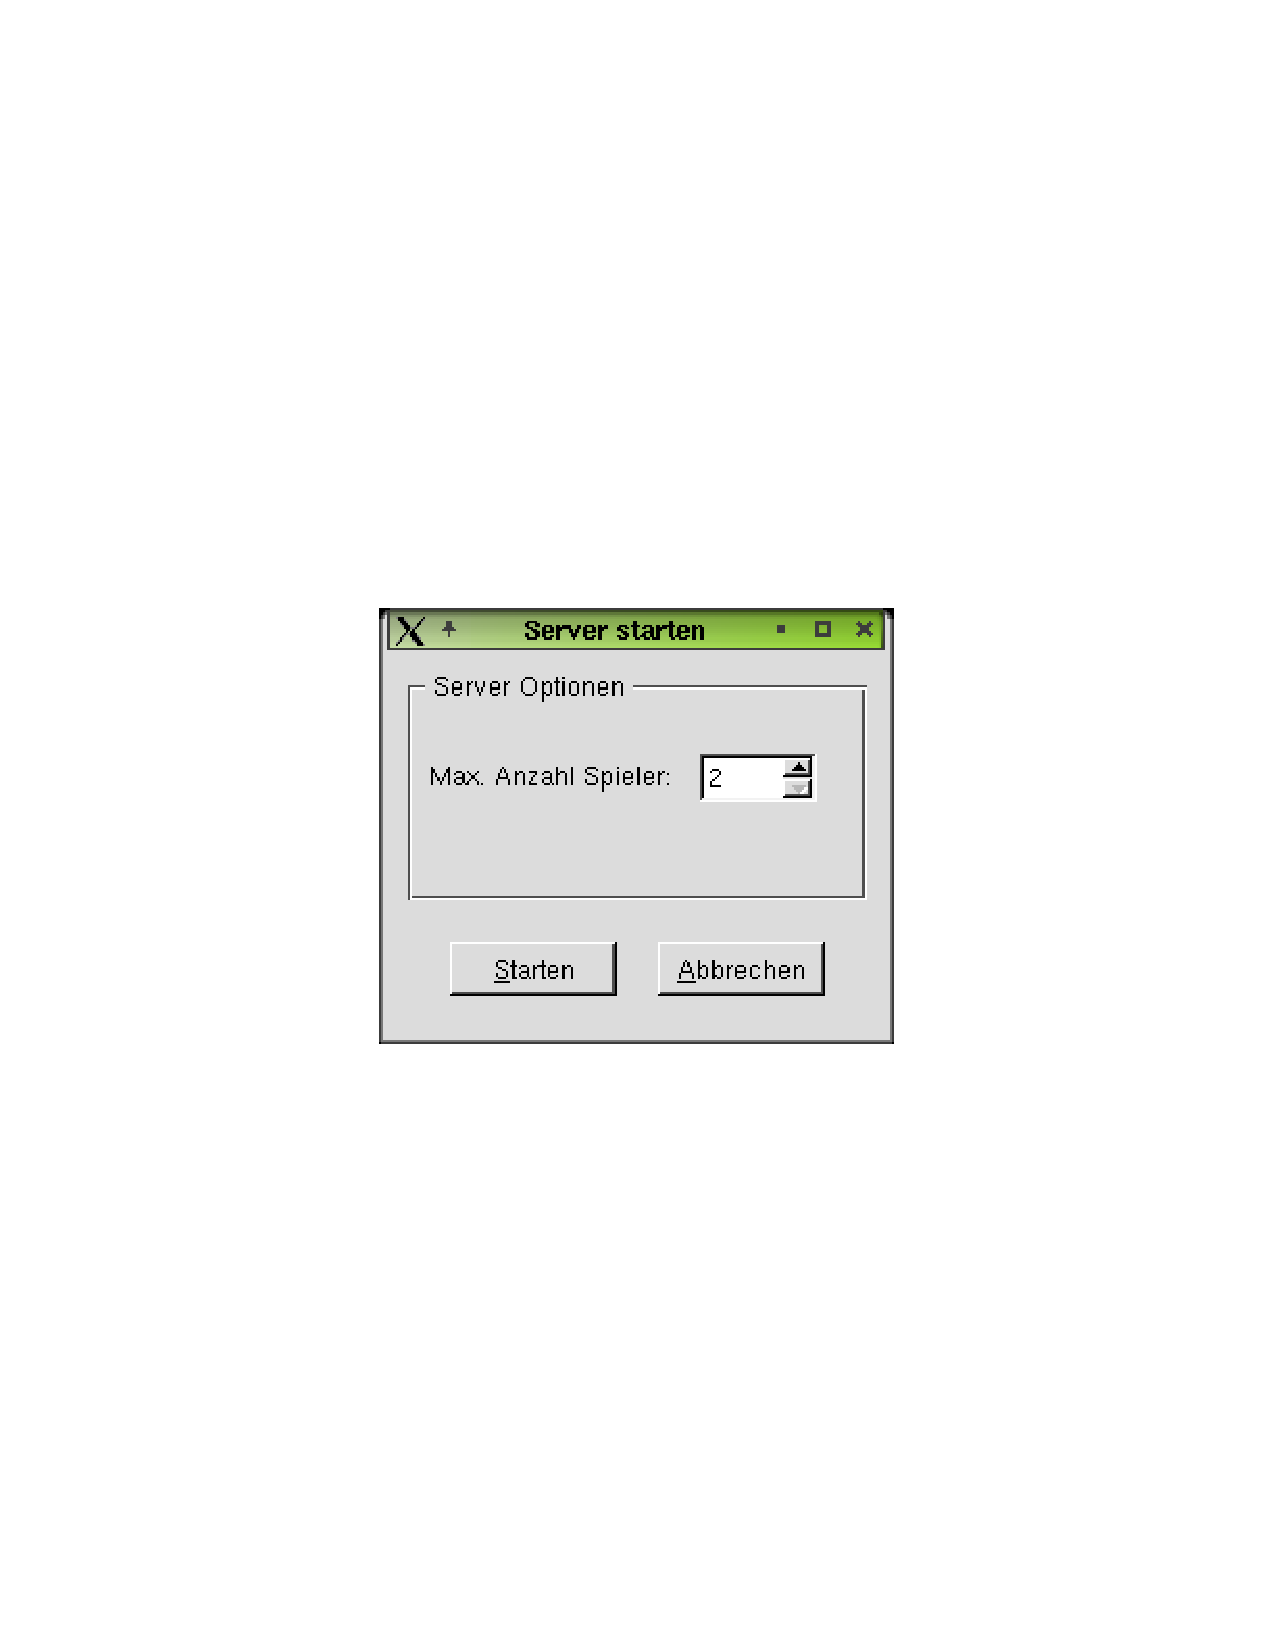
\includegraphics[height=6cm]{./images/startserver.pdf}}
  \end{center}
  \caption{Snapshot des Dialoges Server starten}
\end{figure}

Dieser Dialog dient zum Starten eines Servers.

\begin{figure}[H]
  \begin{center}
    {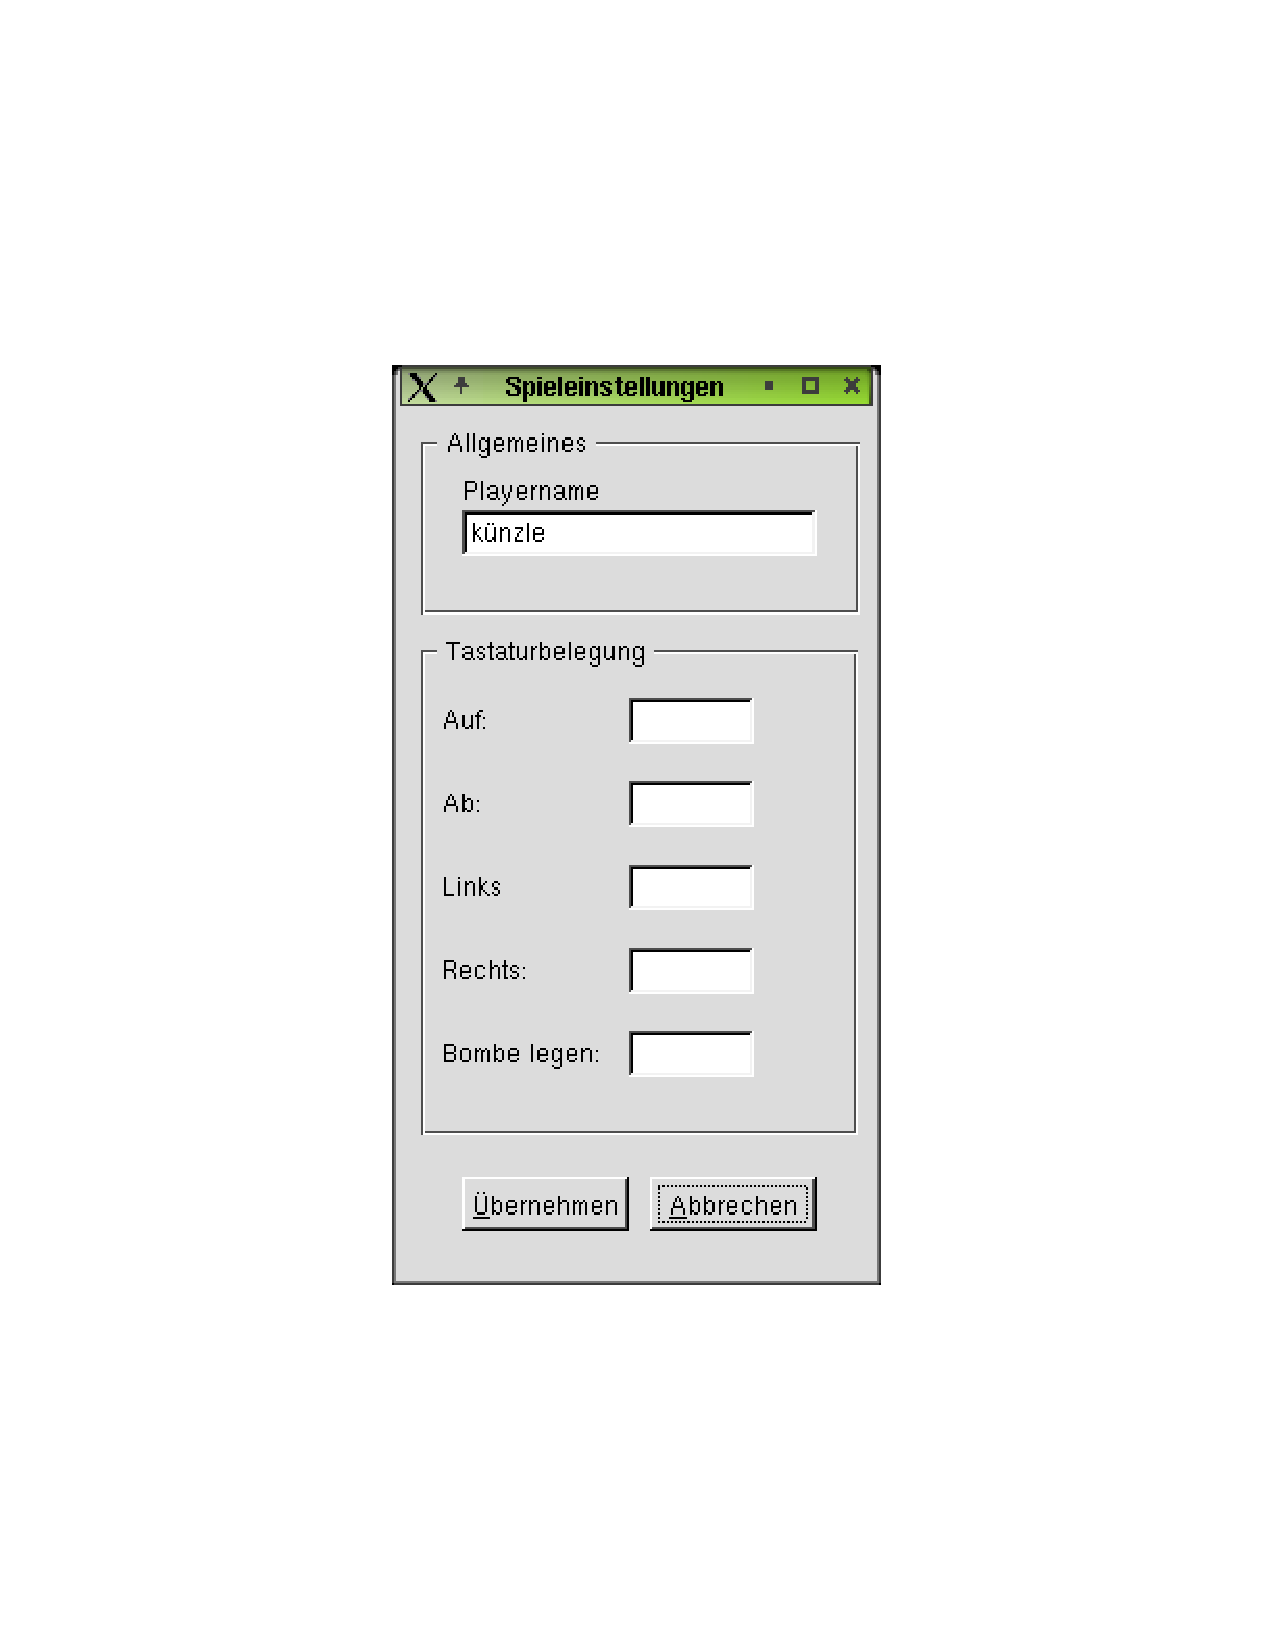
\includegraphics[height=10cm]{./images/settings.pdf}}
  \end{center}
  \caption{Snapshot des Dialoges Einstellungen}
\end{figure}

Dieser Dialog dient prim"ar zum Konfigurieren des Spielernamens.
Leider reichte uns die Zeit nicht mehr, die Tastaturbelegung
variierend zu machen. Vorgesehen war es jedoch in diesem Dialog.


\section{GUI Klassendiagramm}

Das gesamte Klassendiagramm befindet sich im Register Nr. 9.

\section{GUI Sequenzdiagramme}

\begin{figure}[H]
  \begin{center}
    {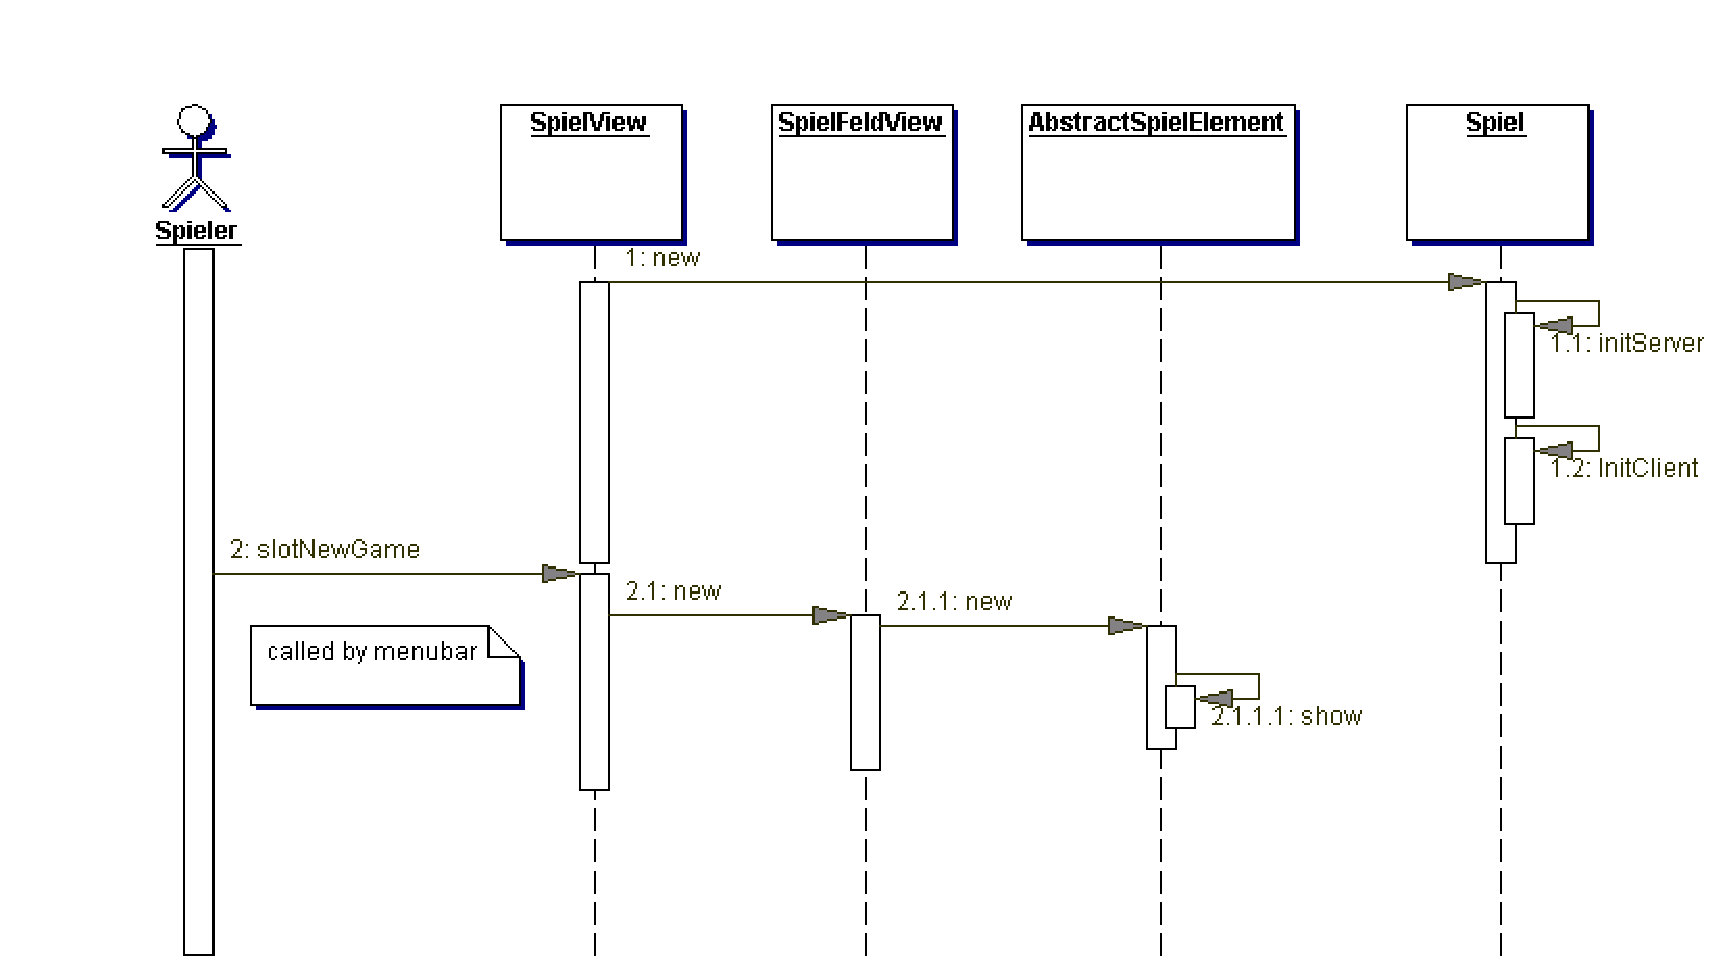
\includegraphics[height=6cm]{./images/neuesSpiel.pdf}}
  \end{center}
  \caption{Sequenzdiagramm f"ur neues Spiel}
\end{figure}



\begin{figure}[H]
  \begin{center}
    {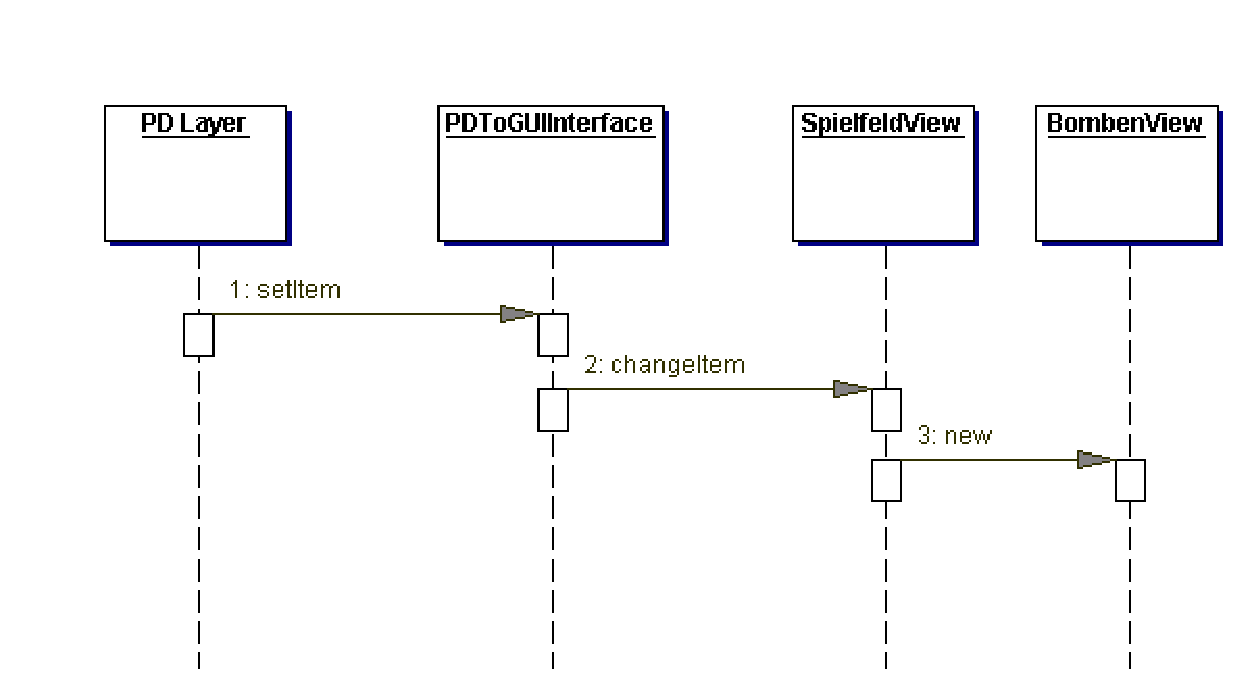
\includegraphics[height=6cm]{./images/bombeLegen.pdf}}
  \end{center}
  \caption{Sequenzdiagramm f"ur Bombe legen}
\end{figure}

Die PD wird hier als Blackbox betrachtet. Diese ruft "uber das
PDToGUIInterface setItem auf, wobei setItem als Parameter
den typ BOMBE und die Koordinaten x und y beinhaltet.
Die PDToGUIInterface Instanz teilt diese Anforderung der SpielfeldView
Instanz mit, welche dann mit dem Erzeugen einer neuen BombenView
Instanz reagiert.

\begin{figure}[H]
  \begin{center}
    {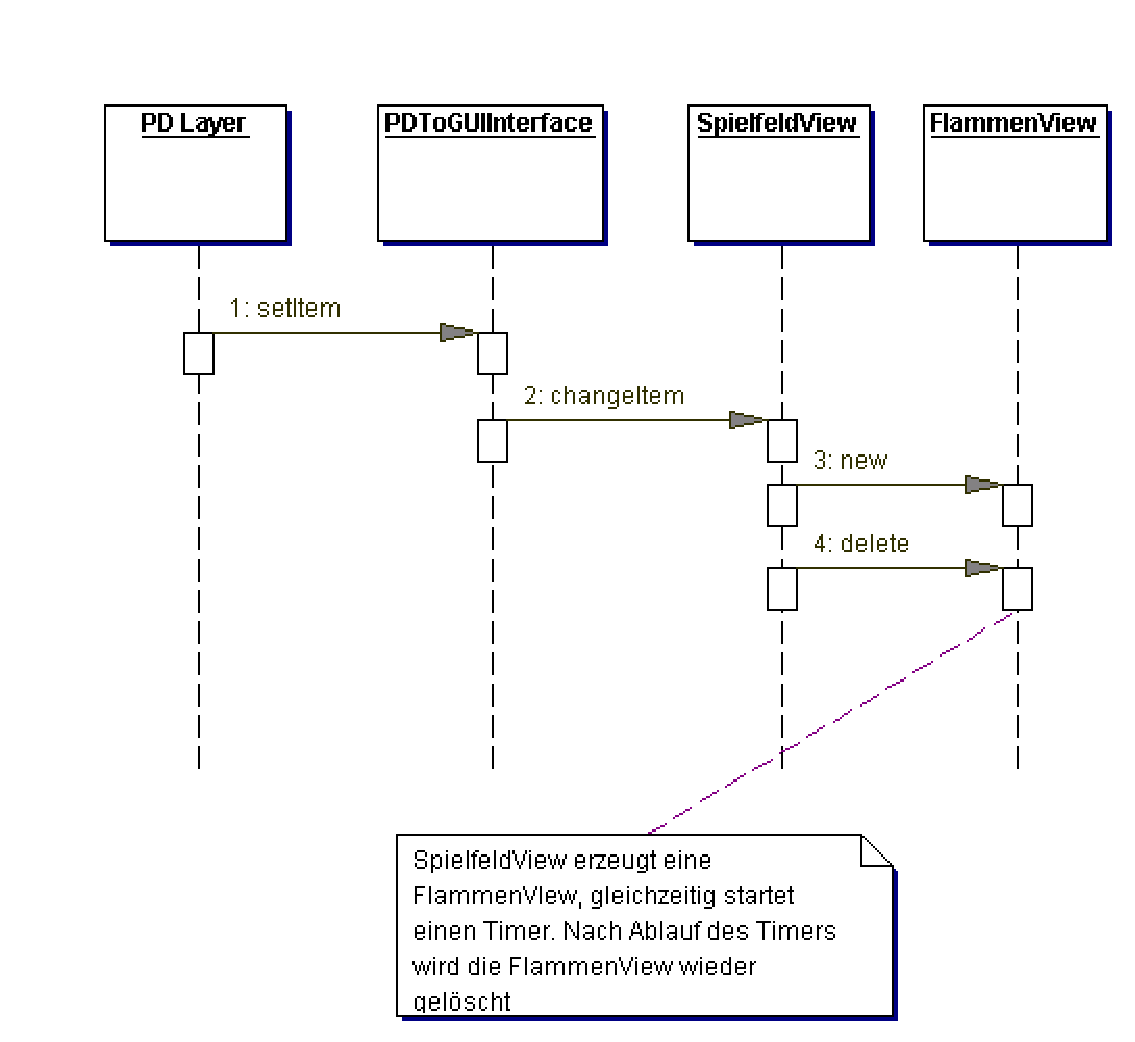
\includegraphics[height=6cm]{./images/neueflamme.pdf}}
  \end{center}
  \caption{Sequenzdiagramm f"ur eine Flamme anzeigen}
\end{figure}

Wieder vom PD Layer her kommt die Anforderung mit einem setItem.
Diesmal mit den Parametern FLAMME als typ und die Koordinaten x und y.
Die PDToGUIInterface Instanz leitet die Anforderung an die Instanz von SpielfeldView
weiter.
Die SpielfeldView Instanz erzeugt danach eine neue FlammenView Instanz. Gleichzeitig
startet einen Timer (QTimer), welcher nach Ablauf den Slot timerDone() aufruft.
In timerDone() wird die FlammenView wieder zerst"ort. Das bewirkt im Spiel selber
das kurze Erscheinen der Flamme, sozusagen explosionsartig.


\section{GUI Klassenbeschreibung}

\subsection{Klasse SpielView}

Die Klasse SpielView enth"alt einzig allein ein Menu. "Uber dieses kann der Spieler
einen Server starten, sich bei einem Server anmelden, Einstellungen vornehmen
und last but not least das Spiel starten bezw. beenden.
Um dies zu erm"oglichen, hat die Klasse SpielView Pointers auf die Klassen
JoinServerView, ServerView und SpielOptView. Diese werden bei den entsprechenden
Slots (Callbacks des Menus), mit show() aufgerufen.
Diese Klasse assoziiert ebenfalls mit der Klasse SpielFeldView, sozusagen
der Hauptklasse des GUIs (siehe unten). Im Konstruktur wird diese erzeugt, jedoch noch
nicht angezeigt. Dies erfolgt erst nachdem der Menupunkt Spiel starten ausgew"ahlt wurde.


\subsection{Klasse SpielFeldView}

Sie ist sozusagen die Kernklasse im GUI Design. Diese Klasse verwaltet alle
sich auf dem Spielfeld befindenen Elementen (Aggregation zu AbstractSpielElementView).
Um das zu erreichen, wird sie von der Klasse QCanvasView abgeleitet. QCanvasView
ist die Pr"asentationsklasse f"ur QCanvasItems, also f"ur einzelne Grafikelementen. Auch das
Keyboard-Eventhandling erfolgt in dieser Klasse. Falls Keyboard-Events auftreten,
werden diese abgefangen, und nur die f"ur das Spiel relevanten Steuersignale werden
der Klasse PDToGUIInterface weitergeleitet, wo sie dann von der PD verarbeitet werden.
Gleichzeitig erh"alt sie von der Klasse GUIToPDInterface Methodenaufrufe, welche das Ver"andern
des UI's zur Folge haben. Dies beinhaltet Items hinzuf"ugen und entfernen (Bombe und Flamme),
die Richtung der Spielfigur festlegen (um das entsprechende Sprite zu laden) und die Figur an
eine andere Koordinate bewegen. Um die Spielfigur eindeutig zu identifizieren, hat die Methode
moveXY() zus"atzlich den Paramter ID, dessen Wert die PD weiss.
Diese Klasse ist fast intelligenzlos. Sie nimmt nur Befehle von der Interfaceklasse entgegen,
oder leitet an diese Steuersignale weiter.

\subsection{Klasse SpielfigurView}

Diese Klasse repr"asentiert die Spielfigur. Sie wird im Konstruktor der Klasse SpielFeldView
erzeugt. Ihre Koordinaten erh"alt sie ebenfalls von der Klasse SpielFeldView.
Um grafisch ansprechende Animationen zu erm"oglichen, ist sie von der Klasse QCanvasSprite
abgeleitet. Diese Klasse erm"oglicht das dynamische Laden von Bildern (Frames), welche
durch entsprechende Methoden zu einer Animation zusammengesetzt werden k"onnen. In der Methode
advance(int step) erfolgt die eigentliche Animation in zwei Schritten: Wenn step 0 ist, hat
man die M"oglichkeit, die Items auf dem Spielfeld auf Kollision zu "uberpr"ufen (collision detection).
Im zweiten Schritt (step ist 1) werden die Items, in unserem Fall die Spielfigur, bewegt.
Diese Methode wird von Qt aufgerufen, vorausgesetzt das setAnimated(true) aiufgerufen wurde.

\subsection{Klasse AbstractSpielElementView}

Diese Klasse wurde von der Klasse QCanvasPolygonalItem abgeleitet. Sie erg"anzt diese
Klasse nur mit den Koordinaten. Gleichzeitig dient sie als Oberklasse f�r alle
auf dem Spielfeld befindenen Elementen, ausser der Spielfigur. Dies ist notwendig,
um die Aggregation zwischen SpielFeldView und AbstractSpielElement zu erreichen.

\subsection{Klasse MauerView}

Sie repr"asentiert auf dem Spielfeld eine unzerst"orbare Mauer. Das Attribut
rtti steht f"ur run time type information. Sie dient zur Identifikation.

\subsection{Klasse BombenView}

Sie repr"asentiert eine Bombe auf dem Spielfeld.

\subsection{Klasse FlammenView}

Sie repr"asentiert eine Flamme auf dem Spielfeld.

\subsection{Klasse ServerView}

Diese Klasse repr"asentiert einen Dialog, "uber welchen
einen Server gestartet werden kann. Als Option kann die
max. Anzahl Spieler festgelegt werden, nach dem Motto
""Server ist K"onig"".
Die Anmeldung erfolgt via den Klassen SpielView und GUIToPDInterface
zur PD mit dem Callback (Slot) bStartenPressed.

\subsection{Klasse JoinServerView}

Diese Klasse repr"asentiert einen Dialog, "uber welchen
sich ein Spieler an einen Server anmelden kann. Das einzige,
was der Spieler tun muss, ist eine g"ultige IP-Adresse
(bei welcher einen NetBomb Server gestartet wurde) eingeben.
Der Anmeldevorgang beginnt nach dem Dr"ucken des Anmelden-Buttons,
bezw. in der Methode bStartenPressed.

\subsection{Klasse SpielOptView}

Sie repr"asentiert einen Dialog, "uber welchen der Spieler
Einstellungen zur Spielersteuerung und seinen Playername
eingeben kann.

\subsection{Klasse GUIToPDInterface}

Sie ist die Kommunikations-Schnittstelle vom GUI zur PD.
Es werden die f"ur das Spiel relevanten Keyboard Events
zur PD weitergeleitet mit keyPressed und keyReleased.
Die PD erh"alt "uber die Schnittstelle die Aufforderung den
Server zu starten mit startServer(). Um sich an einen Server
anzumelden wird dir PD mit joinServer und den Parametern Spielername
bezw. IP  dies entsprechend mitgeteilt.
Um das Spiel schlussendlich zu starten, wird der PD mit startGame()
migeteilt.
Wir w"ahlten das Singleton Pattern der GoF, damit es einerseits nur
einmal instanziert ist, andererseits von jedem beliebigen Ort
zu Verf"ugung steht.

\subsection{Klasse PDToGUIInterface}

"Uber diese Klasse nimmt das GUI die W"unsche der PD entgegen. Alle
Aufrufe gehen danach weiter an die Klasse SpielFeldView.
Auch hier das Singleton Pattern der GoF aus den gleichen Gr"unden wie
bereits erw"ahnt wurde.


%end pd design

%begin pd design

%\section{PD Klassendiagramm}

%\begin{figure}[H]
%  \begin{center}
    %{\rotatebox{90}{\includegraphics[height=...cm]{./images/...}}}
%  \end{center}
%  \caption{Klassendiagramm PD}
%\end{figure}


\section{PD Klassendiagramm}

\begin{figure}[H]
  \begin{center}
    {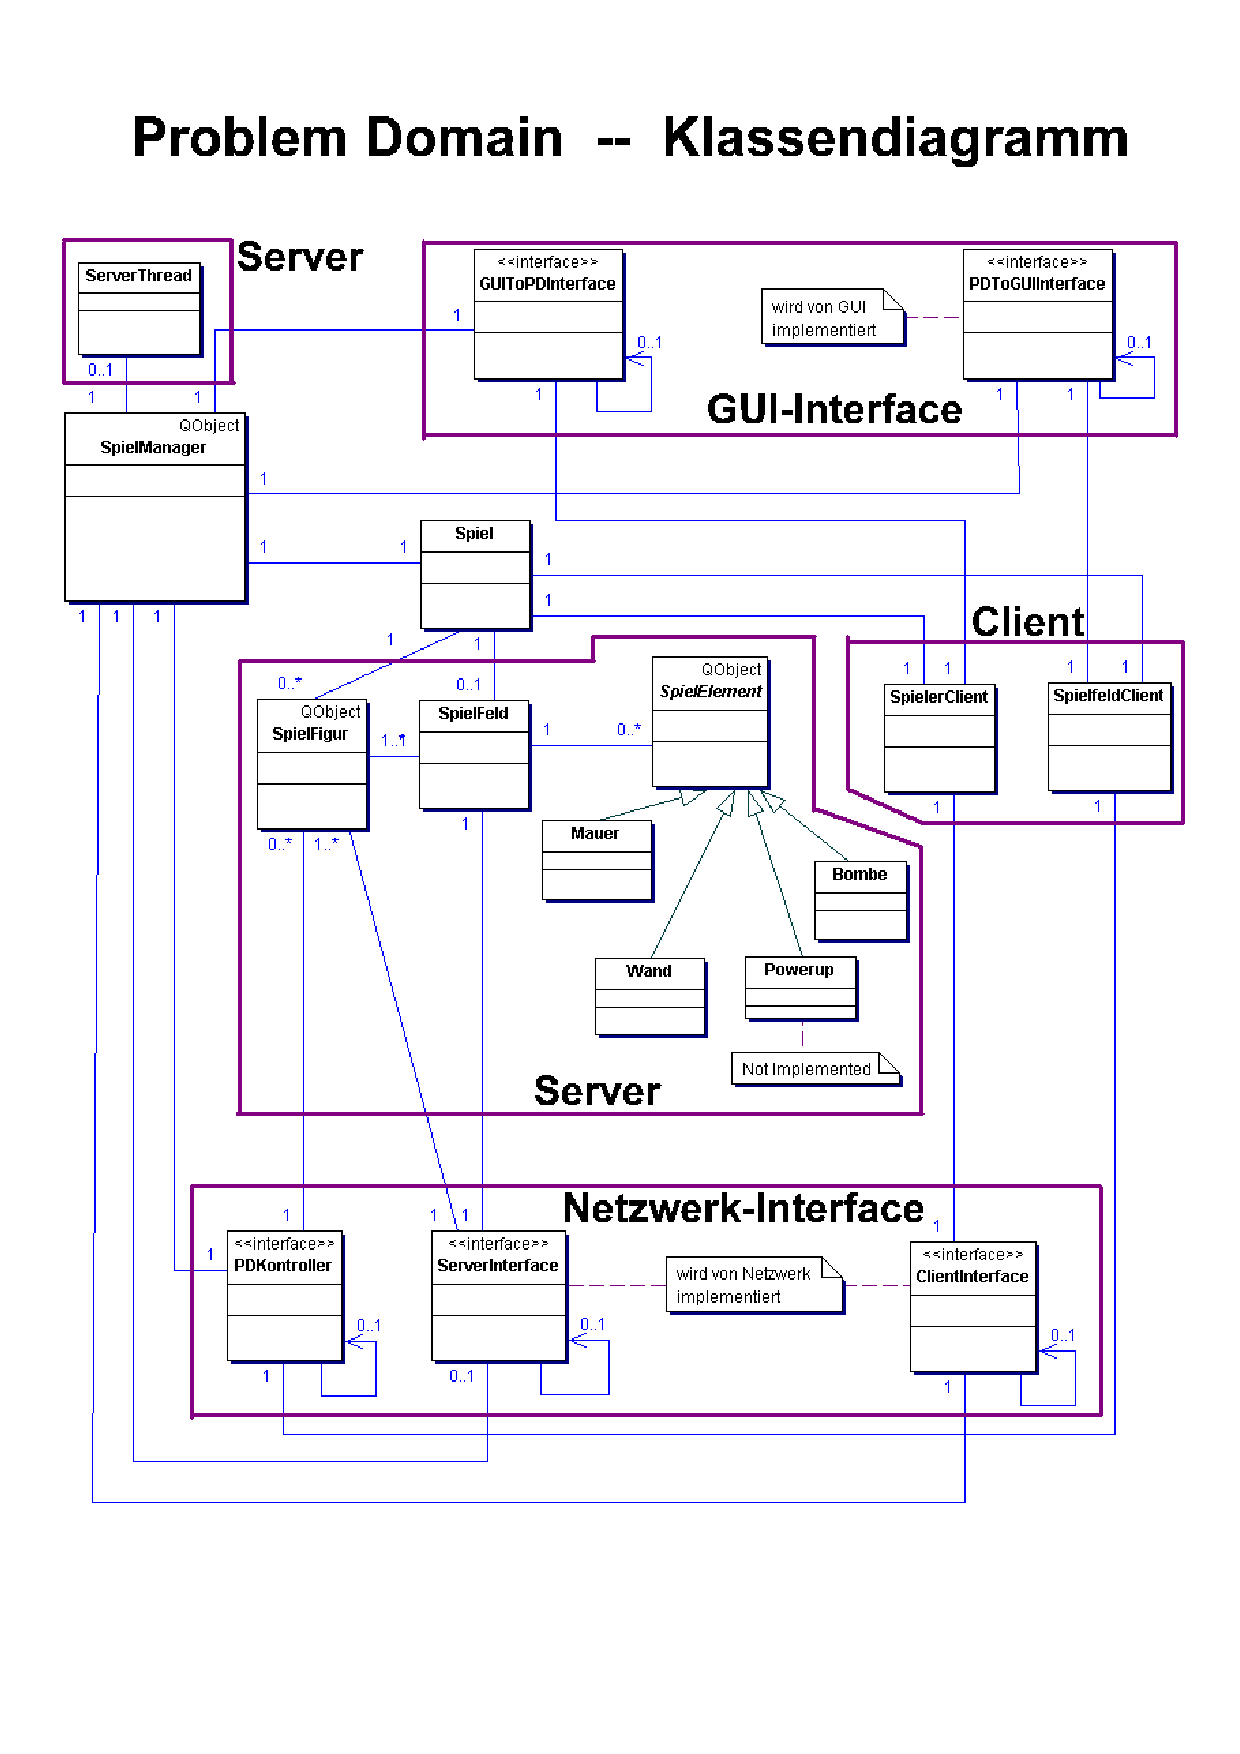
\includegraphics[height=18cm]{./images/pda4g.pdf}}
  \end{center}
  \caption{Klassendiagramm PD (siehe auch A3 Blatt in Register 9)}
\end{figure}

\section{PD Sequenzdiagramme}

\begin{figure}[H]
  \begin{center}
    {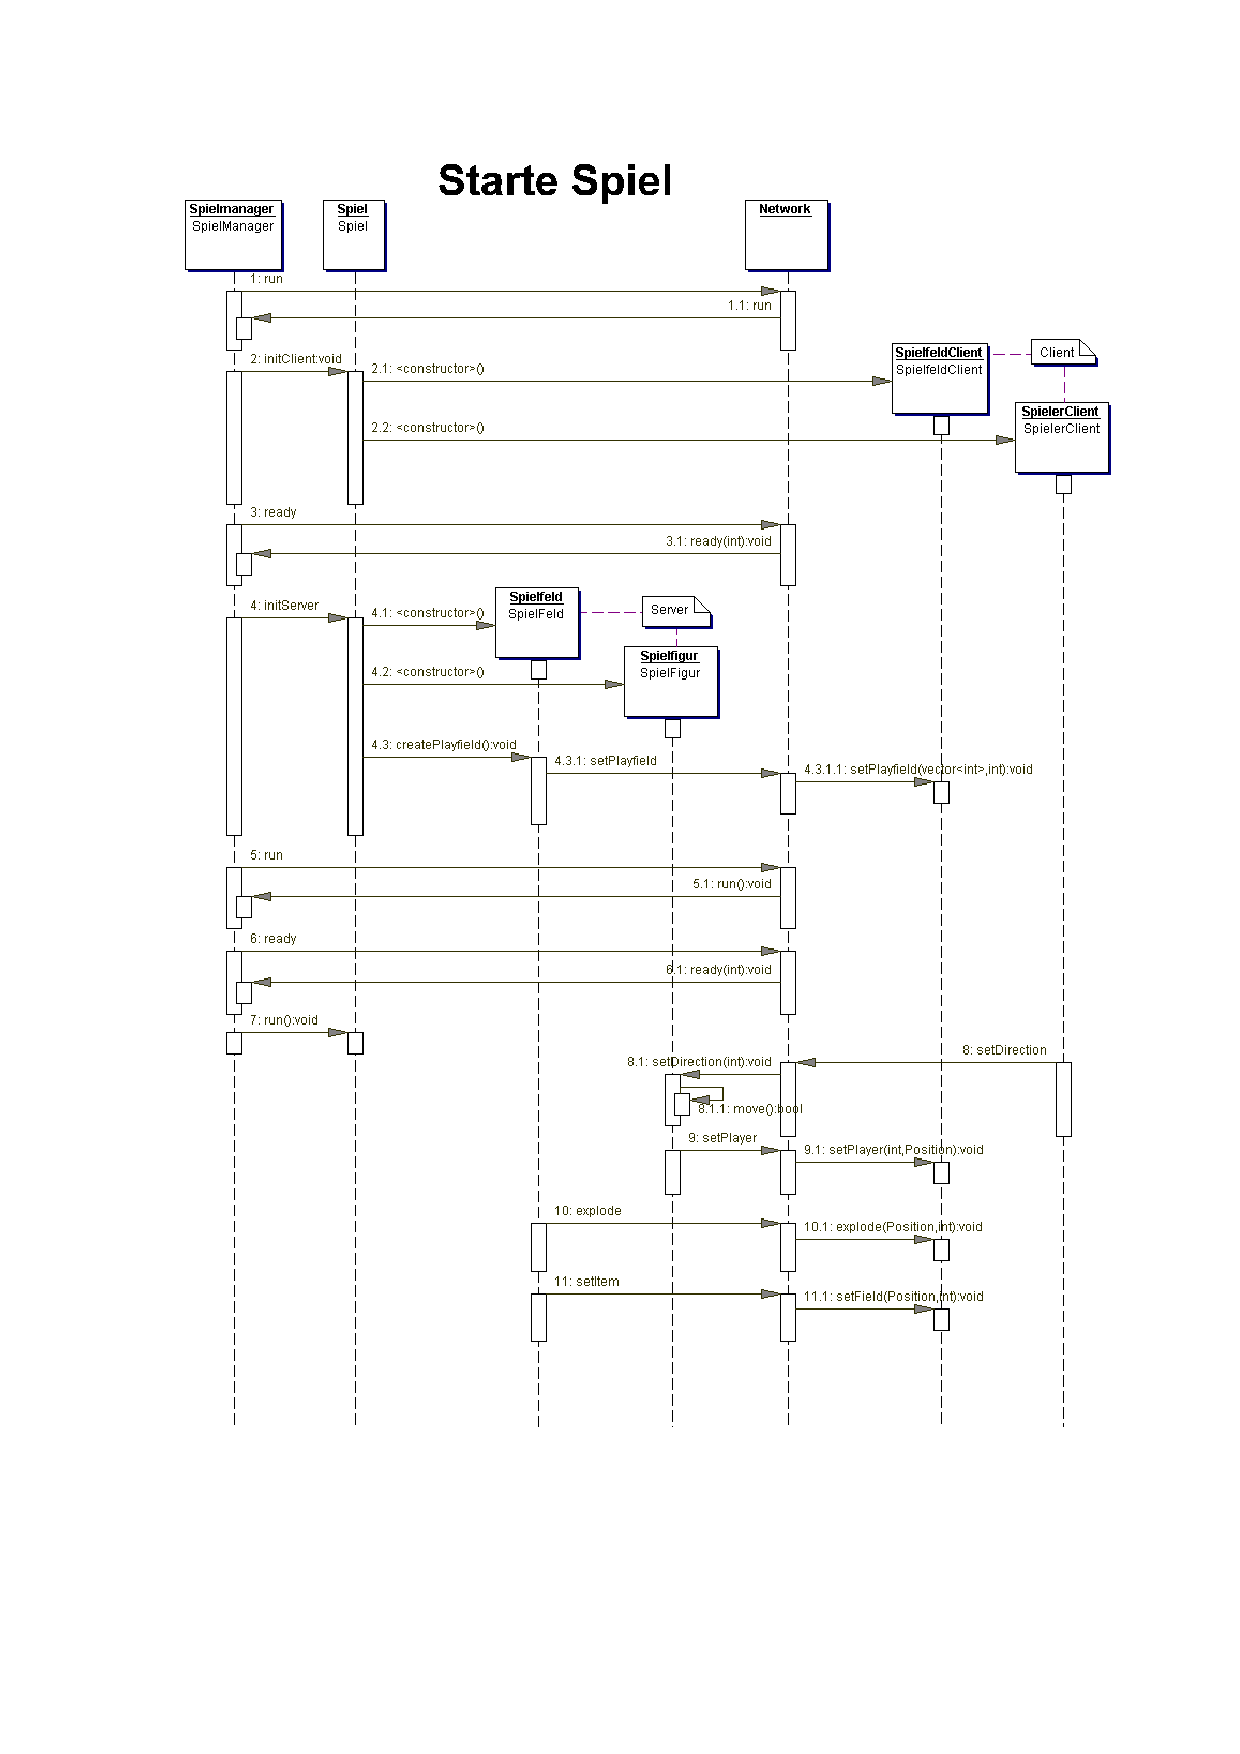
\includegraphics[height=18cm]{./images/startespiel2.pdf}}
  \end{center}
  \caption{Sequenzdiagramm f"ur neues Spiel}
\end{figure}

\begin{figure}[H]
  \begin{center}
    {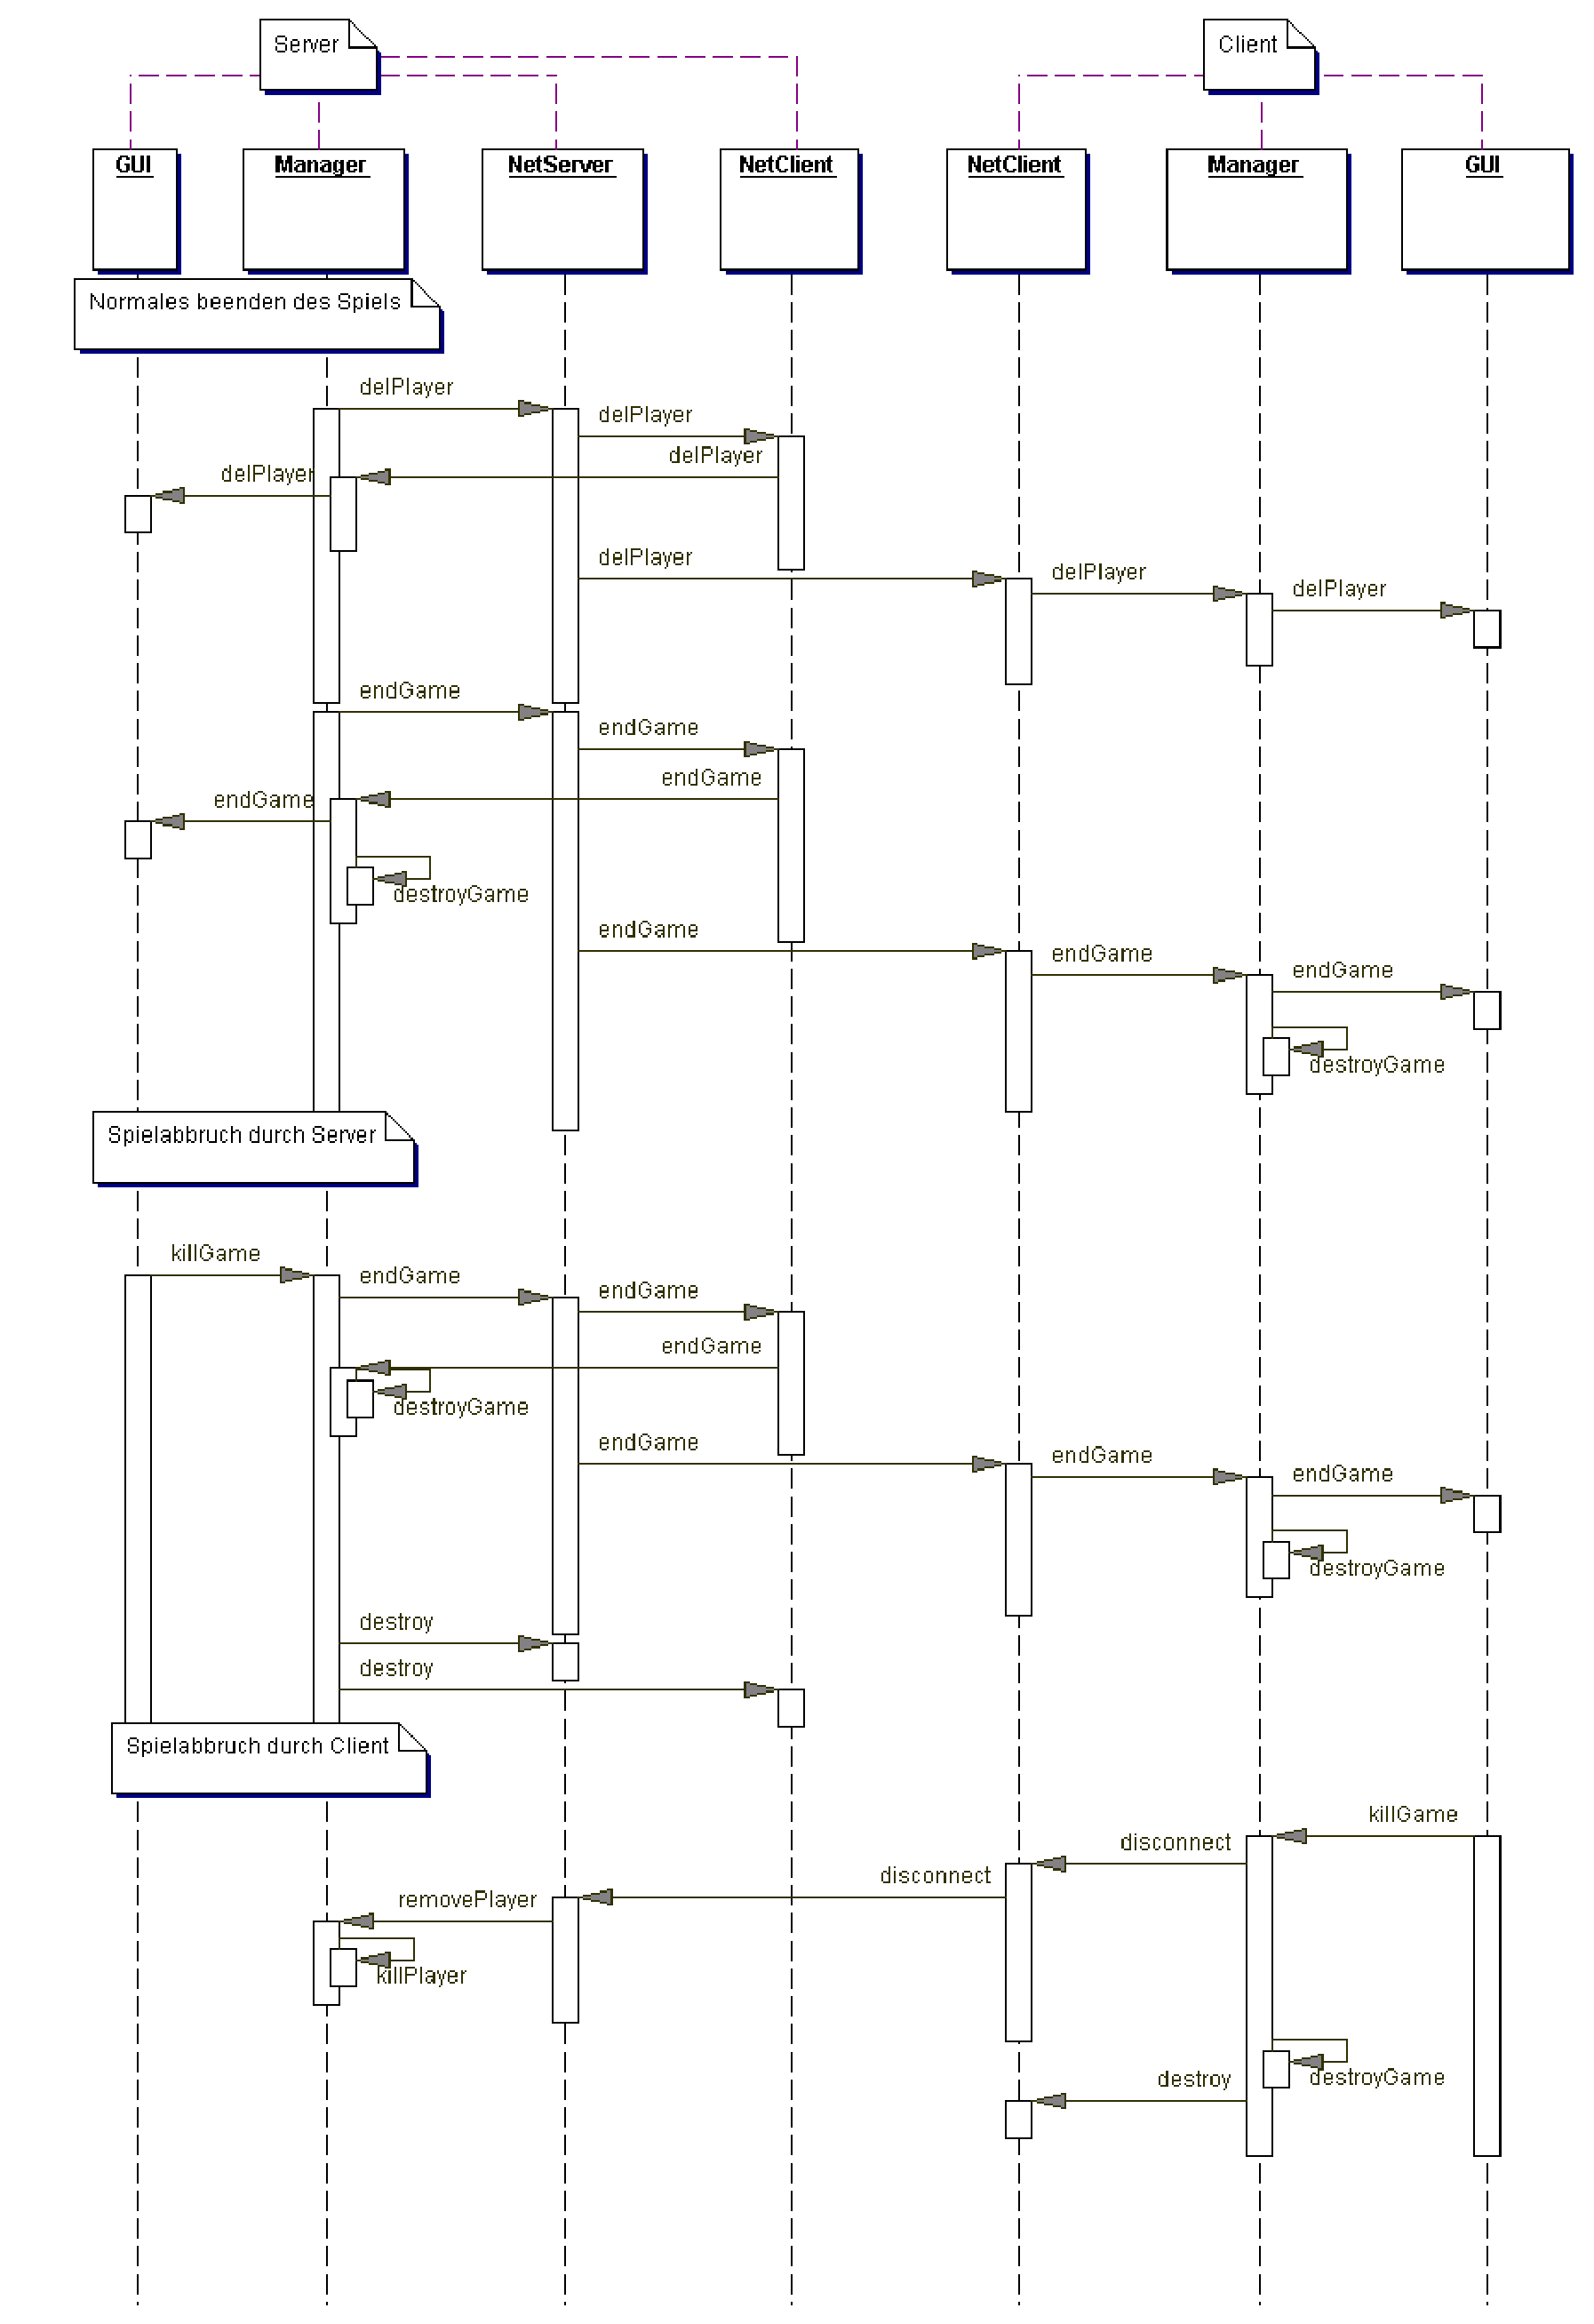
\includegraphics[height=18cm]{./images/endgame.pdf}}
  \end{center}
  \caption{Sequenzdiagramm f"ur das Beenden des Spiels}
\end{figure}

\begin{figure}[H]
  \begin{center}
    {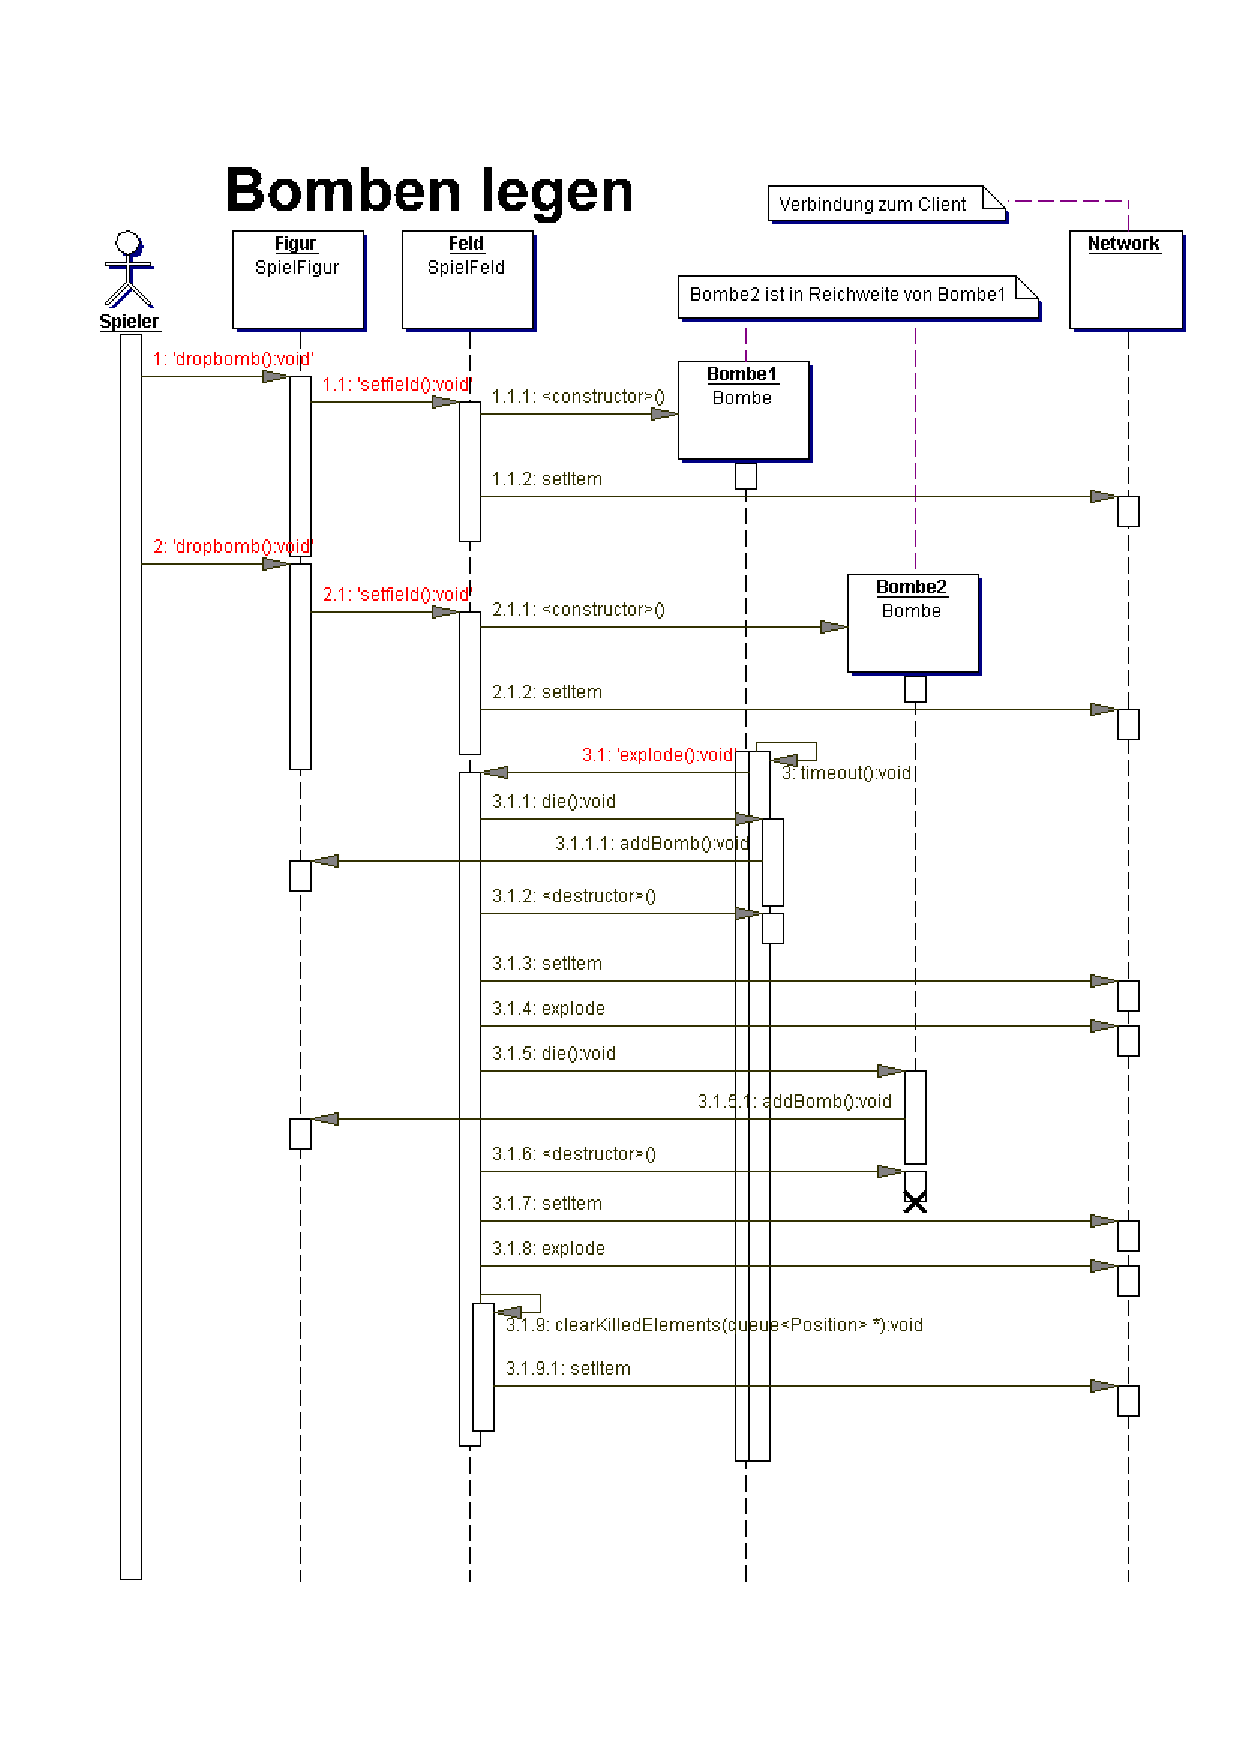
\includegraphics[height=18cm]{./images/bombenlegen.pdf}}
  \end{center}
  \caption{Sequenzdiagramm f"ur das Legen von Bomben}
\end{figure}

% ProblemDomain  Klassenbeschrieb
% 19.4.2002 U.Heimann   Dokument erstellt
% 26.4.2002 U.Heimann   erweitert, korrigiert
%  2.5.2002 U.Heimann   �nderung Client/Server
%  5.6.2002 u.Heimann   �nderung Iteration 2
% 12.7.2002 U.Heimann   Endversion

\section{PD Klassenbeschreibung}
Die endg"ultige Version des Spiels soll "uber ein Netzwerk gespielt werden. Deshalb wird die PD in Server und Client unterteilt.
Die Klassen des Servers sind f"ur die Berechnung des gesamten Spielverlaufs (Positionen, Treffererkennung, ...) verantwortlich.
Der Client konvertiert die Steuerbefehle und schickt sie "uber das Netzwerk an den Server. Der Server berechnet die Auswirkungen
und schickt die "Anderungen zur"uck an alle Clients. Der Client reicht die "Anderungen wiederum an das User Interface weiter.
Jeder Spieler hat auf seinem Rechner eine Instanz des Clients, aber nur einer hat zus"atzlich noch eine Instanz des Servers.

\subsection{Klasse SpielManager}
Der Spielmanager ist f"ur die Verwaltung des Spiels verantwortlich. Er kontrolliert den Verbindungsaufbau
und -abbruch der Clients und erzeugt die zum Spielen notwendigen Objekte.
\subsubsection{Attribute}
\begin{tabular}{p{50mm}p{90mm}}
-serverGame      : bool           &  True wenn dieser PC als Server agiert. \\
-playerConnected : bool[]         &  True wenn mit der entsprechenden ID ein Spieler verbunden ist. \\
-playerName      : string[]       &  Namen der verbundenen Spieler. \\
-playerReady     : bool[]         &  True wenn der Spieler zum Spielen bereit ist. \\
-game            : Spiel*         &  Pointer auf das Spiel-Objekt. \\
-serverThread    : ServerThread*  &  Pointer auf Server-Listening-Thread. \\
-pdMutex         : QMutex*        &  Mutex zum Schutz der PD vor Mehrfachzugriff. \\
-serverMutex     : QMutex*        &  Mutex zum Beenden des Server-Threads. \\
-client          : Client*        &  Pointer auf Client-Objekt, zum Abfragen des Sockets. \\
-clientTimer     : QTimer*        &  Timer zur regelm"assigen Abfrage des Client-Sockets. \\
 & \\
-guiInputInterface      : GUIToPDInterface*  &  Interface  GUI $\rightarrow$ PD \\
-guiOutputInterface     : PDToGUIInterface*  &  Interface  PD  $\rightarrow$ GUI \\
-netInputInterface      : PDKontroller*      &  Interface  NET $\rightarrow$ PD \\
-netOutClientInterface  : ClientInterface*   &  Interface  PD (client) $\rightarrow$ NET \\
-netOutServerInterface  : ServerInterface*   &  Interface  PD (server) $\rightarrow$ NET \\

\end{tabular}
\subsubsection{Funktionen}
\begin{tabular}{p{50mm}p{90mm}}
+startServer(string playerName)        : void  &  Startet den Netzwerk-Server und meldet sich als Spieler an. \\
+joinServer(string ipAddress, string playerName)  : void  &  Startet den Netzwerk-Client und meldet sich beim Server an. \\
+startGame()                           : void  &  Initialisiert und startet das Spiel mit den verbundenen Spielern. \\
+endGame()                             : void  &  Beendet das laufende Spiel. \\
+killGame()                            : void  &  Bricht das laufende Spiel ab. (zu irgendeinem Zeitpunkt) \\
+errorMsg(int msgNr, string addInfo)   : void  &  Bearbeitet Fehlermeldungen vom Netzwerk. \\
 & \\
+newPlayer(int playerID, string playerName) : void  &  Ein neuer Spieler hat sich beim Server angemeldet. \\
+removePlayer(int playerID)            : void  &  Entfernt einen Spieler aus der Spielerliste und entfernt ihn aus dem Spiel. \\
+ready(int playerID)                   : void  &  Setzt den Spieler spielbereit. \\
+distributeMsg(string info)            : void  &  Schickt eine Nachricht an alle verbundenen Clients weiter. \\
 & \\
+connectConfirm()                      : void  &  Best"atigt die Verbindung zum Server. \\
+setPlayerName(int playerID, string name) : void &  Setzt den Namen eines Verbundenen Spielers. \\
+disconnect()                          : void  &  Meldet sich beim Server ab. \\
+run()                                 : void  &  Synchronisiert und startet das Spiel. \\
+infoMsg(string info)                  : void  &  Zeigt eine Nachricht vom Server an. \\
 & \\
-createNetworkServer()                 : void  &  Startet den Server-Listening-Thread. \\
-killNetworkServer()                   : void  &  Beendet den Server-Listening-Thread. \\
-createNetworkClient()                 : void  &  Startet den Client-Timer zur Abfrage des Sockets. \\
-killNetworkClient()                   : void  &  Beendet den Client-Timer. \\
 & \\
-clientTimeout()                       : void  &  wird bei Ablauf des Client-Timers aufgerufen. \\
\end{tabular}


\subsection{Klasse Spiel}
Die Klasse Spiel erzeugt die restliche Spielstruktur (Spielfeld, Spielfiguren) je nach Anzahl
Spieler. Es wird immer ein Client erstellt, und beim Spielf"uhrer zus"atzlich noch ein Server. Sie ist daf"ur verantwortlich,
dass das Spiel mit allen Clients synchronisiert ist bevor das Spiel gestartet wird. \\
\subsubsection{Attribute}
\begin{tabular}{p{50mm}p{90mm}}
-serverFeld  :  Spielfeld*         &  Pointer auf das ServerSpielfeld. \\
-figur[4]    :  Spielfigur*        &  Pointer auf die Spielfiguren des Servers. \\
-clientFeld  :  SpielfeldClient*   &  Pointer auf das ServerSpielfeld. \\
-spieler     :  SpielerClient*     &  Pointer auf die Spielfigur des Clients. \\
\end{tabular}

\subsubsection{Funktionen}
\begin{tabular}{p{50mm}p{90mm}}
+initClient()             : void  &  Initialisiert die Client-Umgebung. \\
+initServer(bool activPlayers[], string playerNames[]) : void  &  Initialisiert die Server-Umgebung. \\
+ready()                  : bool  &  gibt TRUE zur"uck wenn Client bereit ist. \\
+run()                    : void  &  Synchronisiert und startet das Spiel. \\
+killPlayer(int playerID) : void  &  Entfernt einen Spieler vom Spielfeld. \\
-destroyClient()          : void  &  R"aumt die Client-Umgebung nach Spielende auf. \\
-destroyServer()          : void  &  R"aumt die Server-Umgebung nach Spielende auf. \\
\end{tabular}


\subsection{Klasse GUIToPDInterface (Singleton)}
"Uber diese Schnittstelle sendet das User Interface die Tastatureingaben des Spielers an die PD.\\
\subsubsection{Attribute}
\begin{tabular}{p{50mm}p{90mm}}
-manager : SpielManager*   &  Pointer auf den Spielmanager. \\
-spieler : SpielerClient*  &  Pointer auf den Spieler. \\
-pdMutex : QMutex*         &  Sichert die PD vor Mehrfachzugriff ab. \\
\end{tabular}
\subsubsection{Funktionen}
\begin{tabular}{p{50mm}p{90mm}}
+setManager(SpielManager* man, QMutex* pdMut) : void  &  Registriert den Spielmanager. \\
+setPlayer(SpielerClient* player): void  &  Registriert den Spieler. \\
+startServer(const char* player) : void  &  Startet neues Spiel als Server. \\
+joinServer(const char* ipAdress, const char* playerName) : void  &  Startet neues Spiel als Client. \\
+startGame()                     : void  &  Startet das Spiel mit den verbundenen Spielern (nur Server) \\
+killGame()                      : void  &  Beendet das Spiel zu einem beliebigen Zeitpunkt. \\
+keyPressed(int key)             : void  &  Eine Taste wurde gedr"uckt. \\
+keyReleased(int key)            : void  &  Eine Taste wurde losgelassen. \\
\end{tabular}

\subsection{Klasse PDToGUIInterface (Singleton)}
"Uber diese Schnittstelle sendet die PD die "Anderungen des Spielfeldes an das User Interface.
(siehe GUI) \\

\subsection{Klasse ServerInterface}
(siehe Netzwerk)

\subsection{Klasse ClientInterface}
(siehe Netzwerk)

\subsection{Klasse ServerThread}
Separater Thread f"ur die Abfrage des Server-Sockets. (Abgeleitet von QThread) \\
\subsubsection{Attribute}
\begin{tabular}{p{50mm}p{90mm}}
-runServer : QMutex*  &  Synchronisationsobjekt zum Beenden des Serverthreads. \\
-pdMutex   : QMutex*  &  Sichert die PD vor Mehrfachzugriff ab. \\
\end{tabular}
\subsubsection{Funktionen}
\begin{tabular}{p{50mm}p{90mm}}
+run()     : void     &  Ausf"uhrungsroutine des Threads. \\
\end{tabular}

\subsection{Klasse PDKontroller (Singleton)}
Der PDKontroller empf"angt und verarbeitet die Nachrichten vom Netzwerk. Sie ist als Singleton realisert und ist die Schnittstelle
vom Netzwerk zu der PD.
\subsubsection{Attribute}
\begin{tabular}{p{50mm}p{90mm}}
-spielManager : SpielManager*     &  Pointer auf den Manager. \\
-serverFigur  : Spielfigur*[]    &  Pointer auf die Spielfiguren (nur Server) \\
-clientFeld   : SpielfeldClient*  &  Pointer auf das Spielfeld. \\
\end{tabular}
\subsubsection{Funktionen}
\begin{tabular}{p{50mm}p{90mm}}
+setManager(SpielManager* manager) : void  &  Registriert den Spielmanager. \\
+setSpielfigur(int playerID, Spielfigur* figur) : void  &  Registriert eine Spielfigur. \\
+setClientFeld(SpielfeldClient* feld) : void  &  Registriert das Spielfeld. \\
Manager-Funktionen & \\
+newPlayer(int playerID, string playerName) : void  &  Ein neuer Spieler hat sich beim Server angemeldet. \\
+disconnect(int playerID)              : void  &  Ein Spieler hat sich abgemeldet. \\
+disconnect()                          : void  &  Der Server hat sich abgemeldet. \\
+ready(int playerID)                   : void  &  Der Spieler ist spielbereit. \\
+run()                                 : void  &  Spielstart  \\
+endGame()                             : void  &  Beendet das Spiel. \\
+connectConfirm()                      : void  &  Best"atigt die Verbindung zum Server. \\
+receiveMsg(string msg)                : void  &  Empf"angt eine Nachricht vom Server. \\
+receiveMsg(int playerID, string msg)  : void  &  Empf"angt eine Nachricht vom Client (zum Verteilen an alle Clients). \\
+errorMsg(int msgNumber, string addInfo) : void  & Empf"angt eine Fehlermeldung vom Netzwerk. \\
+setPlayerName(int playerID, string name) :  &  Setzt den Namen eines Spielers. \\
Server-Funktionen & \\
+setDirection(int direction, int playerID) : void  &  Setzt neue Laufrichtung des Spielers. \\
+setBombPressed(bool keypressed, int playerID) : void   &  Setzt das Bomben-lege-Flag. \\
Client-Funtionen & \\
+setPlayfield(vector<int> feldinfo, int zeilenbreite) : void  &  Initialisiert das ganze Spielfeld. \\
+setItem(Position position, int item) : void  &  Setzt ein einzelnes Objekt auf dem Spielfeld. \\
+setPlayer(int playerID, Position position) : void  &  Setzt die Position einer Spielfigur. \\
+delPlayer(int playerID) : void  &  L"oscht einen Spieler vom Spielfeld. \\
+explode(Position position, int reichweite) : void  &  L"ost eine Explosion auf dem Spielfeld aus. \\
\end{tabular}


\subsection{Klasse Spielfeld}
Die Klasse Spielfeld enth"alt ein Array das den aktuellen Zustand und die Positionen aller Spielelemente representiert. Sie hat
Zugriff auf alle spielentscheidenden Informationen. \\
\subsubsection{Attribute}
\begin{tabular}{p{50mm}p{90mm}}
-feld         : Spielelement*[]         &  Abbild des aktuellen Spielstandes. Jeder Eintrag im Array entspricht einem Feld. d.h.
                                           es k"onnen nicht mehrere Elemente auf einem Feld sein. (Spielfiguren werden hier
                                           nicht gespeichert!) \\
-player       : Spielfigur[]            &  Zeigerliste auf alle Spielfiguren des aktuellen Spiels. Die Position der Figur ist
                                           bei der Figur gespeichert.\\
-game         : Spiel*                  &  Pointer auf das Spiel-Objekt. \\
-netInterface : ServerInterface*        &  Pointer zum Netzwerk-Interface des Servers. \\
-minPlayers   : int                     &  Sind weniger Spieler als minPlayers auf dem Feld wird das Spiel beendet. \\
\end{tabular}
\subsubsection{Funktionen}
\begin{tabular}{p{50mm}p{90mm}}
+startGame() : void  &  Startet das Spiel. \\
+stopGame() : void  &  Beendet das Spiel. \\
+setField(Position pos, int item, Spielfigur* figur = NULL) : void  &  Setzt ein bestimmtes Element an die Koordinate (x,y). \\
+getField(Position pos) : int item        &  Liefert das Element das sich an der Koordinate (x,y) befindet. \\
+setPlayer(int playerID, Spielfigur* player) : void     &  Meldet einen neuen Spielfigur beim Spielfeld an. \\
+delPlayer(int playerID) : void  &  Meldet den Spieler ab. \\
+explode(Position pos, int reichweite, queue<Position>* toDie = NULL) : void  &  Berechnet die Explosion. \\
-clearKilledElements(queue$<$Position$>$* toDie) : void  &  L"oscht die gesprengten Elemente vom Spielfeld. \\
\end{tabular}

\subsection{Klasse Spielfigur}
Die Klasse Spielfigur enth"alt alle wichtigen Informationen "uber Position und Zustand der Spielfigur. \\
\subsubsection{Attribute}
\begin{tabular}{p{50mm}p{90mm}}
-spielfeld     : Spielfeld*       &  Pointer auf das Spielfeld-Objekt. \\
-pdKontroller  : PDKontroller*    &  Pointer auf den den PD-Kontroller. F"ur ankommende Meldungen vom Netzwerk. \\
-netInterface  : ServerInterface* &  Pointer auf das Netzwerk-Interface. F"ur abgehende Meldungen ans Netzwerk. \\

-playerID      : int       &  Spielernummer  \\
-playerName    : string    &  Name des Spielers. \\
-position      : Position  &  Position der Spielfigur auf dem Spielfeld in (x,y) Koordinaten. \\
-direction     : int       &  Richtung in die die Spielfigur gehen m"ochte. (STAY, UP, DOWN, LEFT, RIGHT) \\
-numberOfBombs : int       &  Die Anzahl Bomben die er noch legen darf. -1 wenn Bombe gelegt wurde, +1 wenn seine Bombe explodiert ist
                              oder ein Bomben-Powerup aufgenommen wurde. \\
-reichweite    : int       &  Reichweite der Bombe in Feldern. Wird der Bombe "ubergeben wenn sie gelegt wird. Wird erh"oht, wenn ein
                              Flammen-Powerup aufgenommen wird. \\
-alive         : bool      &  TRUE wenn die Spielfigur noch lebt. \\
-bombPressed   : bool      &  TRUE wenn die Bomben-lege-Taste gedr"uckt ist. \\
-moveTimer     : QTimer*   &  Timer f"ur die Bewegungs-Verz"ogerung. \\
\end{tabular}
\subsubsection{Funktionen}
\begin{tabular}{p{50mm}p{90mm}}
+setDirection(int dir)          : void   &  Setzt die Laufrichtung der Spielfigur (STAY, UP, DOWN, LEFT, RIGHT). \\
+setBombPressed(bool bomb)      : void   &  Setzt das bombPressd Flag (bomben-lege-Taste gedr"uckt). \\
+getName()                      : string &  Liefert den Namen des Spielers. \\
+getPosition()                : Position &  Liefert die aktuelle Position der Spielfigur. \\
+addBomb()                      : void   &  F"ugt eine Bombe zum Arsenal der Spielfigur hinzu. \\
+wakeup()                       : void   &  Erweckt die Spielfigur zum Leben, erlaubt ihr sich zu bewegen. \\
+die()                          : void   &  Zerst"ort die Spielfigur wenn sie gesprengt wurde. \\
+move()                         : bool   &  Bewegt die Spielfigur um ein Feld in die aktuelle Richtung (direction). \\
+getReichweite()                : int    &  Gibt die Reichweite zur"uck. \\
-dropBomb()                     : void   &  Legt eine Bombe an der aktuellen Position sofern noch Bomben im Arsenal. \\
-checkField(int posx, int posy) : int    &  Pr"uft ob ein Feld auf dem Spielfeld passierbar ist oder nicht. \\
-timerDone()                    : void   &  Wird aufgerufen wenn der moveTimer abgelaufen ist. \\
\end{tabular}

\subsection{Klasse SpielerClient}
Die Klasse Spieler empf"angt die Benutzereingaben, bestimmt die daraus folgenden Aktionen und leitet sie an den Server weiter.\\
\subsubsection{Attribute}
\begin{tabular}{p{50mm}p{90mm}}
-guiInterface : GUIToPDInterface*  &  Pointer zum GUI-Interface, zum Empfang der Benutzereingaben. \\
-netInterface : ClientInterface*   &  Pointer zum Netzwerk-Interface, zum Versenden der Aktionen. \\
-keylist      : bool[5]            &  Speichert die Informationen welche Tasten momentan gedr"uckt sind. \\
-oldDirection : int                &  Die zuletzt "ubermittelte bewegungsrichtung. \\
\end{tabular}
\subsubsection{Funktionen}
\begin{tabular}{p{50mm}p{90mm}}
+keyPressed(int key) : void      &  Eine Taste wurde gedr"uckt. \\
+keyReleased(int key) : void     &  Eine Taste wurde losgelassen. \\
-computeDirection() : void       &  Berechnet die Laufrichtung aus den Daten der keylist und sendet sie an den Server. \\
\end{tabular}

\subsection{Klasse SpielfeldClient}
Die Klasse SpielfeldClient hat ein vereinfachtes Abbild der Spielsituation gespeichert. Sie ben"otigt dieses zur
berechnung der Explosionen. Sie empf"angt alle "Anderungen vom Server und gibt sie ans GUI weiter.\\
\subsubsection{Attribute}
\begin{tabular}{p{50mm}p{90mm}}
-guiInterface   : PDToGUIInterface*  &  Pointer zum GUI-Interface, zum Senden der "Anderungen. \\
-pdKontroller   : PDKontroller*      &  Pointer zum PD-Kontroller, zum Empfangen der Spielfeld"anderungen. \\
-field          : int[][]            &  Vereinfachtes Abbild der Spielsituation. \\
-playerPosition : Position[4]        &  Die Positionen der Spieler auf dem Spielfeld. \\
-readySet       : bool               &  TRUE wenn bereit zum spielen. \\
\end{tabular}
\subsubsection{Funktionen}
\begin{tabular}{p{50mm}p{90mm}}
+setPlayfield(vector<int> feldinfo, int zeilenbreite) :  void  &  Setzt das gesamte Spielfeld. \\
+setField(Position pos, int item)       : void  &  Setzt ein bestimmtes Element an die Koordinate (x,y). \\
+setPlayer(int playerID, Position pos)  : void  &  Setzt die Spielfigur (nr) an die Position (x,y). \\
+delPlayer(int playerID)                : void  &  L"oscht einen Spieler vom Spielfeld. \\
+explode(Position pos, int reichweite)  : void  &  berechnet eine Explosion. \\
\end{tabular}

\subsection{Klasse SpielElement}
Oberklasse aller auf dem Spielfeld platzierbaren Elemente wie Mauer, Wand, Bombe und Powerup (ausser den Spielfiguren). \\
\subsubsection{Attribute}
\begin{tabular}{p{50mm}p{90mm}}
-position    : Position  &  Position des Elements. \\
-elementType : int       &  Typ des Elements. \\
\end{tabular}
\subsubsection{Funktionen}
\begin{tabular}{p{50mm}p{90mm}}
+die()     : SpielElement*  &  Rein Virtuelle Funktion die beim sprengen des Objekts aufgerufen wird. \\
+getType() : int            &  Liefert den Typ des Elements. \\
\end{tabular}

\subsection{Klasse Mauer}
Die Mauer ist vom Spielelement abgeleitet. Sie kann durch eine Explosion nicht zerst"ort werden. Sie hat keine
spezielle Funktionalit"at.\\

\subsection{Klasse Wand}
Die Wand ist vom Spielelement abgeleitet. Sie kann durch eine Explosion zerst"ort werden und erzeugt dabei ev. ein Powerup. \\
\subsubsection{Attribute}
\begin{tabular}{p{50mm}p{90mm}}
-powerupType : int  &  Typ des versteckten Powerups. \\
\end{tabular}
\subsubsection{Funktionen}
\begin{tabular}{p{50mm}p{90mm}}
+getPowerupType() : int  &  Liefert den Typ des versteckten Powerups. \\
\end{tabular}

\subsection{Klasse Bombe}
Die Bombe ist vom Spielelement abgeleitet. Beim Erzeugen startet der Timer, der am Ende eine Explosion und damit
die Zerst"orung der Bombe einleitet. Sie kann durch eine Explosion zerst"ort werden und explodiert dabei selbst. \\
\subsubsection{Attribute}
\begin{tabular}{p{50mm}p{90mm}}
-dropper      : Spielfigur*  &  Pointer auf die Spielfigur die sie erzeugt hat. \\
-playfield    : Spielfeld*   &  Pointer auf das Spielfeld auf dem sie liegt. \\
-explodeTimer : QTimer*      &  Timer zur Verz"ogerung der Explosion. \\
-reichweite   : int          &  Die Reichweite der Explosion, wird beim Erzeugen gesetzt. \\
\end{tabular}
\subsubsection{Funktionen}
\begin{tabular}{p{50mm}p{90mm}}
+getReichweite() : int   &  Liefert die Reichweite der Bombe. \\
-timeout()       : void  &  wird vom Timer aufgerufen wenn er abgelaufen ist. L"ost die Explosion aus. \\
\end{tabular}


%end pd design

% Begin Netzwerk Interface  Design
\section{Netzwerk Interface}

\begin{figure}[H]
  \begin{center}
    {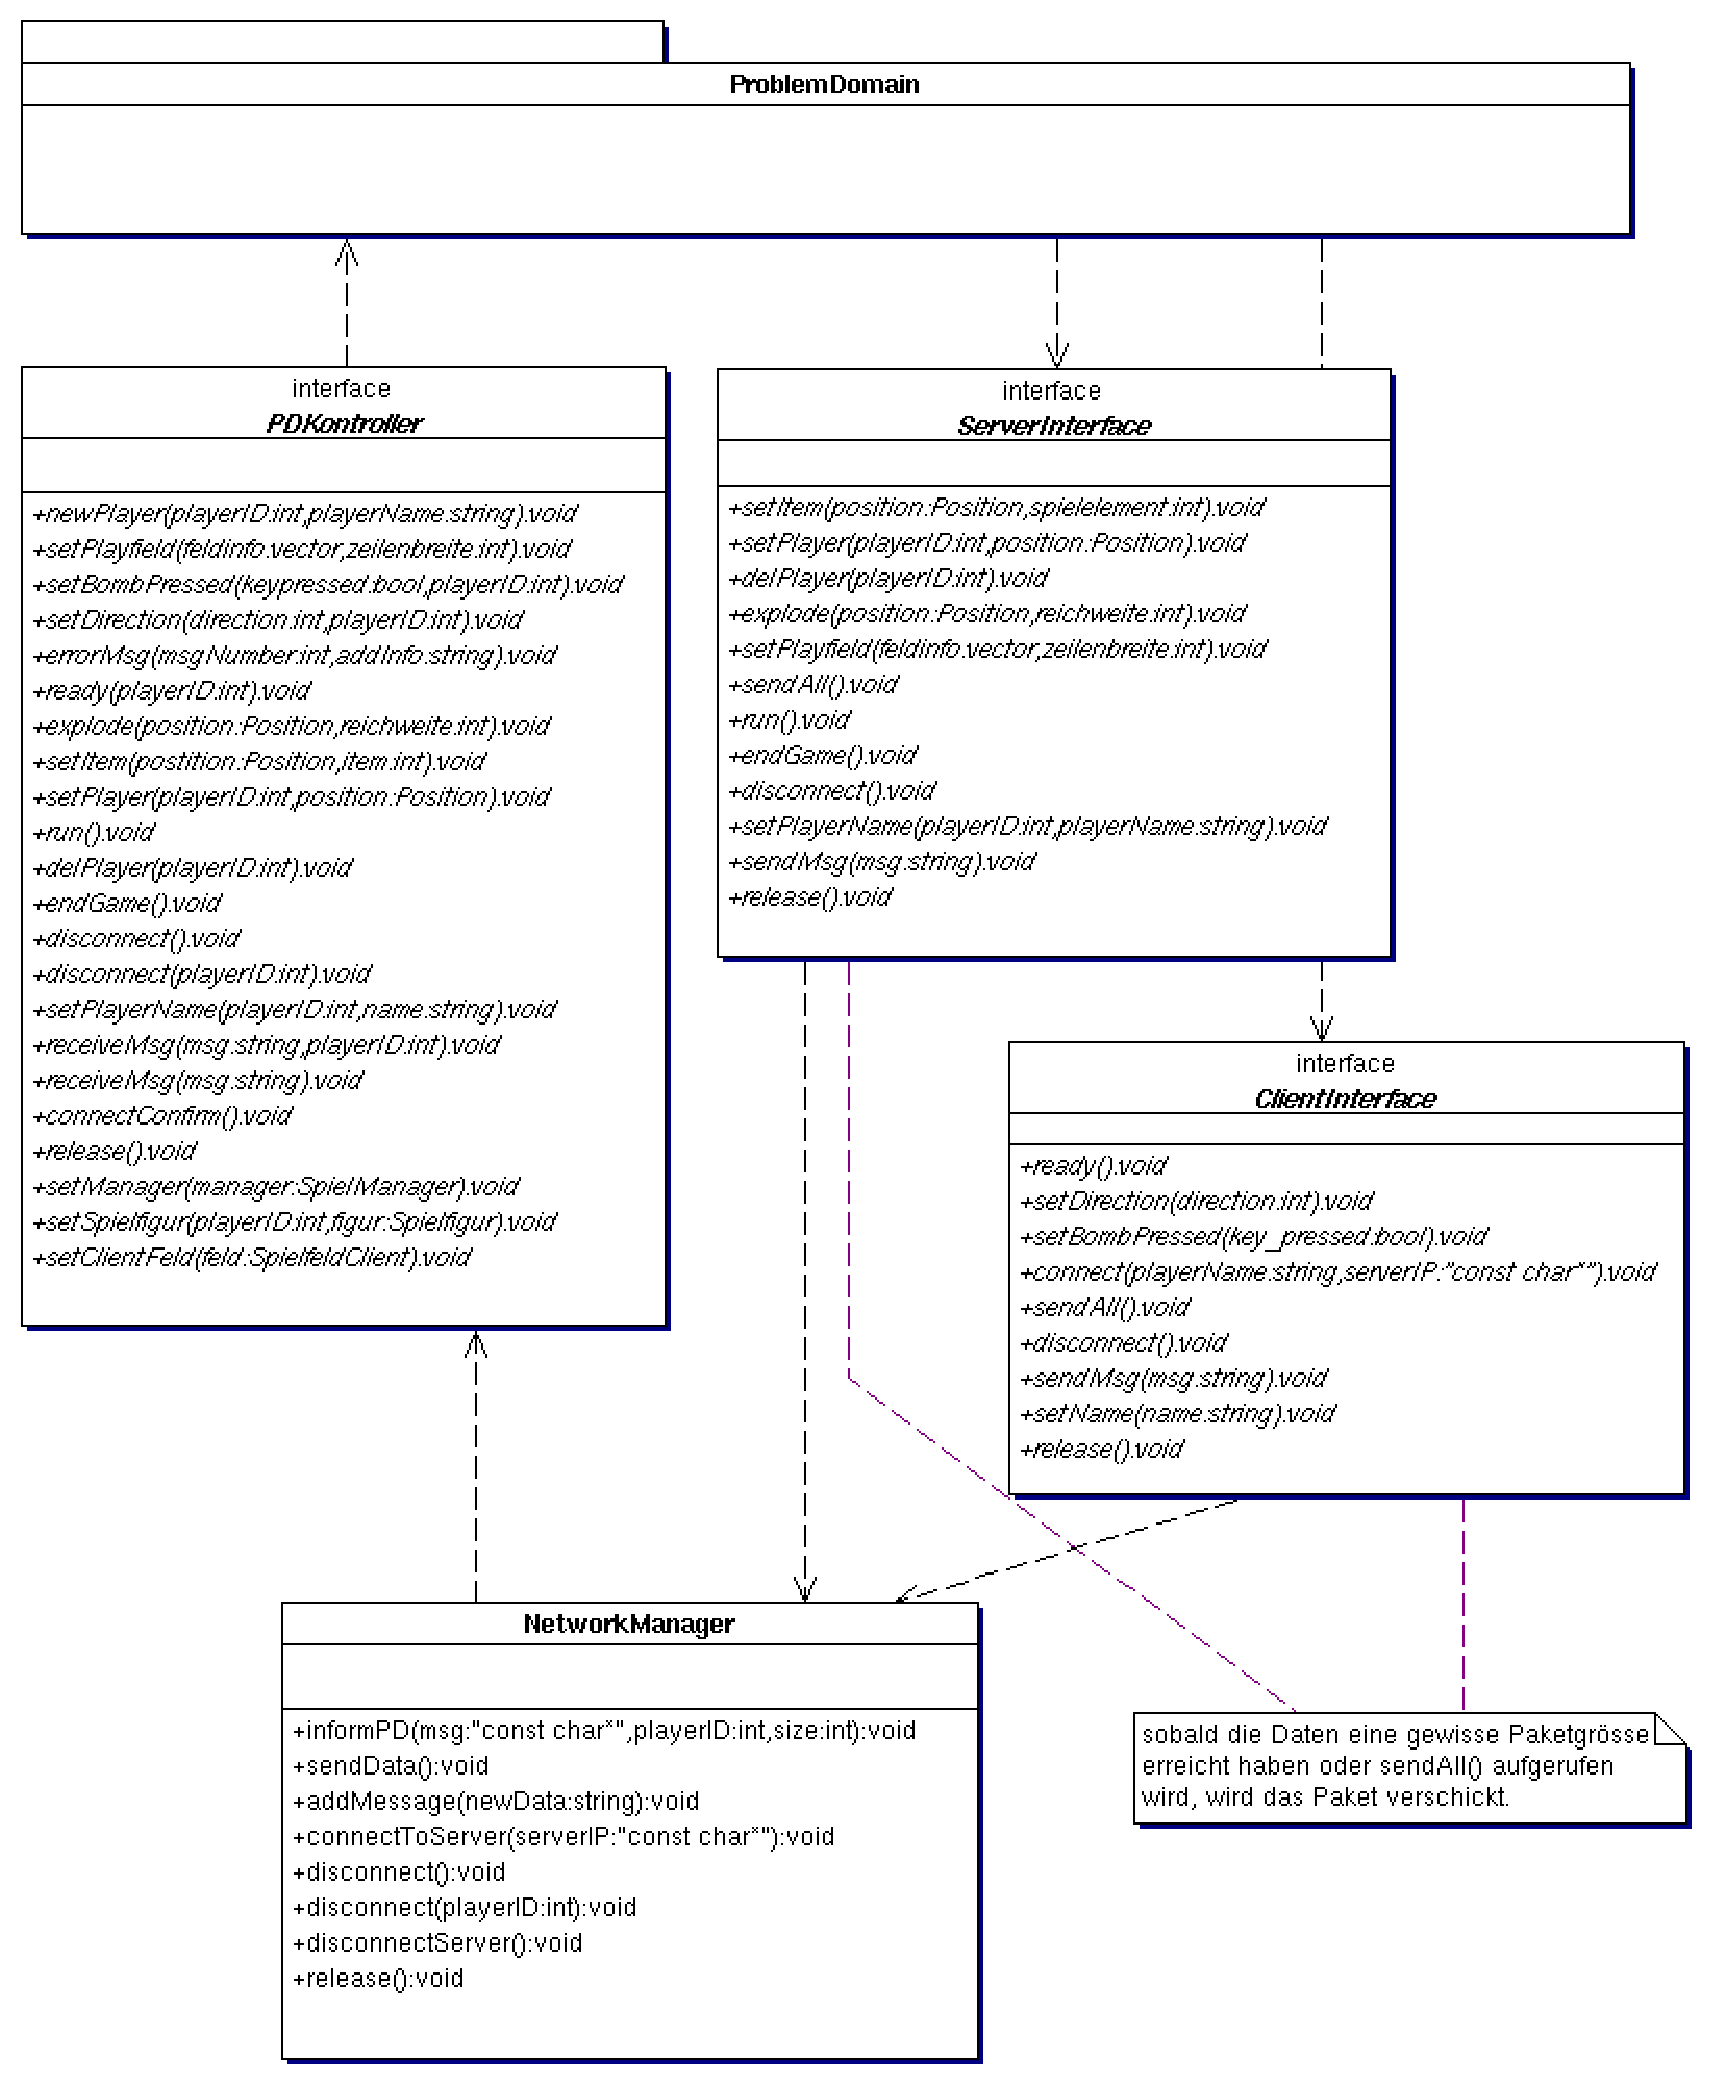
\includegraphics[height=20cm]{./images/netinterface.pdf}}
  \end{center}
  \caption{Interface zwischen Problem Domain und Netzwerk}
\end{figure}

Der Problem Domain stehen die als Singleton implementierten Klassen ServerInterface
und Clientinterface zur Verf"ugung. Die Problem Domain eines Servers verwendet ausschliesslich
das ServerInterface, um mit allen mitspielenden Clients zu kommunizieren. \\
Die Problem Domain eines Clients benutzt das ClientInterface, um sich bei dem Spielserver
anzumelden und ihm Ereignisse zu melden.\\
Die Klassen ServerInterface und ClientInterface rufen ihrerseits Methoden 
der Klasse NetworkManager auf, welcher mit dem Netzwerk kommuniziert. 
Der NetworkManager wird von der Netzwerkschicht aufgerufen und ruft selbst Methoden aus
der Klasse PDKontroller auf.\\
Die Schnittstelle generiert einen tempor"aren String der verschiedene Protokollmessages 
enth"alt. Welche Protokollmessages eingepackt werden ist davon abh"angig, welche Methoden
des Serverinterfaces oder des Clientinterfaces aufgerufen wurden.\\
Dieses Paket wird abgeschickt, sobald es eine gewisse L"ange erreicht hat, oder die Problem Domain
dies durch einen Methodenaufruf ausl"ost.

\section{Netzwerk Interface Klassenbeschreibung}

Verwendete Konstante aus global.h zur Konfiguration des Verhaltens der Schnittstelle:
\\MAX\_STRING\_PAKET\_SIZE. "Ubersteigt der tempor"ar angelegte String der die Nutzdaten 
enth"alt diese L"ange, wird er nach dem Einpacken der letzten Protokollmessage automatisch
verschickt. Zum sofortigen Versenden der Daten kann sowohl im Serverinterface als auch im
Clientinterface die Methode sendAll() aufgerufen werden.
Als Singleton enth"alt diese Klasse auch eine Methode getServerInterface die einen Pointer
auf die Schnittstelle zur"uckgibt.

\subsection{Klasse ServerInterface}
Diese Klasse wird von der Problem Domain des Spielservers benutzt, um Informationen an alle
Spielclients zu schicken. 
Sie ist nach dem Singleton Pattern implementiert.

\subsubsection{Funktionen}
\begin{tabular}{p{50mm}p{90mm}}
+setItem(Position \_pos,int spielelement):void 		 &ein einzelnes Spielelement wird platziert\\
+setPlayer(int playerID, Position \_pos):void 		 &die Spielfigur eines Spielers wird plaziert\\
+delPlayer(int playerID):void;				 &ein Spieler wird aus dem Spiel entfernt\\
+explode(Position \_pos,int reichweite):void		 &signalisiert den Spielclients das Explodieren einer Bombe\\
+setPlayfield(vector$<$int$>$ feldinfo,int zeilenbreite):void&verschickt Spielfelddaten; feldinfo enth"alt Spielelemente;
							  zeilenbreite gibt die Anzahl Felder in einer Horizontalen
							  des Spielfeldes an\\
+sendAll():void 				 	 &l"ost das Versenden des zusammengesetzten Datenpaketes aus\\
+getServerInterface(): ServerInterface*		         &gibt eine Instanz des Serverinterfaces zur"uck\\
+run():void &Startet das Spiel auf den Clients\\
+endGame():void &Signalisiert den Clients das Spielende\\
+disconnect():void&Meldet den Server bei den Clients ab\\
+setPlayerName(int playerID,string playerName):void&Informiert die Clients "uber den Namen eines Spielers\\
+sendMsg(string msg):void&Verschickt an alle Clients eine Nachricht\\
+release():void&l"oscht den Singleton, wenn es keine Referenzen mehr darauf gibt\\
\end{tabular}

\subsection{Klasse ClientInterface}
Das Clientinterface wird von der Problem Domain des Spielclients benutzt, um
Informationen an den Server zu schicken. Sie ist nach dem Singleton Pattern
implementiert.
Als Singleton enth"alt diese Klasse auch eine Methode getClientInterface die einen Pointer
auf die Schnittstelle zur"uckgibt.

\subsubsection{Funktionen}
\begin{tabular}{p{50mm}p{90mm}}
+ready():void 		 &Spielclient meldet sich bereit\\
+setDirection(int direciton):void 		 &Der Server wird "uber die Ausrichtung der Figur informiert\\
+setBombPressed(bool key\_pressed):void;				 &Signalisiert, dass der Spieler Bomben legt\\
+connect(string playerName, const char* serverIP):void		 &Nimmt eine Verbindung zum Spielserver auf\\
+setName(string player\_name):void&Setzt auf dem Server den Spielernamen\\
+sendAll():void 				 	 &l"ost das Versenden des zusammengesetzten Datenpaketes aus\\
+getClientInterface(): ClientInterface*&gibt eine Instanz des Clientinterfaces zur"uck\\
+release():void&l"oscht den Singleton, wenn es keine Referenzen darauf mehr gibt\\
+disconnect():void&Meldet den Client beim Server ab\\
+sendMsg(string msg):void&f"ugt dem tempor"aren Nachrichtenpaket(siehe \ref{Nachrichtenpaket})
 eine Nachricht(siehe \ref{Nachricht}) hinzu\\
\end{tabular}


\subsection{Klasse NetworkManager}
Der NetworkManager wird vom ClientInterface und dem ServerInterface verwendet, um
mit dem Netzwerk zu interagieren. Er speichert die zu versendenden Nachrichten
bis das Nachrichtenpaket eine gewisse Gr"osse hat (s.h. Nachrichtenpaket) oder
dies von einem Interface verlangt wird.\\
Er erh"alt "ubers Netzwerk Nachrichtenpakete und wertet sie aus. Die erhaltene
Information verwendet er um entsprechende Methoden im PDKontroller aufzurufen.
Als Singleton enth"alt diese Klasse auch eine Methode getNetwrokManager die einen Pointer
auf die Schnittstelle zur"uckgibt.

\subsubsection{Funktionen}
\begin{tabular}{p{50mm}p{90mm}}
+getNetworkManager(): NetworkManager*&gibt eine Instanz des NetworkManagers zur"uck\\
+sendData():void&verschickt das zusammengesetzte Nachrichtenpaket(siehe \ref{Nachrichtenpaket}) an den Server\\
+sendServerData():void&verschickt das zusammengesetzte Nachrichtenpaket(siehe \ref{Nachrichtenpaket}) an alle Clients\\
+addMessage(string newData):void&f"ugt dem Nachrichtenpaket(siehe \ref{Nachrichtenpaket}) eine Nachricht (siehe \ref{Nachricht})
	hinzu\\
+informPD(const char* msg,int playerID,int size):void&interpretiert das Nachrichtenpaket(siehe \ref{Nachrichtenpaket}) und ruft die
  entsprechenden Methoden in der Klasse PDKontroller auf\\
+connectToServer(const char* serverIP):void&stellt eine Verbindung zum Server her\\
+release():void&l"oscht den Singleton, wenn es keine Referenz mehr darauf gibt\\
+disconnect():void&Meldet den Client beim Server ab\\
+disconnect(int playerID):void&informiert die PD, falls ein Client nicht mehr erreicht werden kann \\
+disconnectServer():void&ist eine bereitgestellte Methode f"ur das Abmelden des Servers\\
\end{tabular}


\subsection{Klasse StringConverter}
Der StringConverter ist eine Klasse die vom ServerInterface und dem ClientInterface
benutzt wird um Nachrichtencodes und -daten in Pakete zu packen.\\
Der NetworkManager verwendet diese Klasse, um die Nachrichtenpakete wieder
auszupacken und zu interpretieren. Dabei werden Zahlenwerte in Hexadezimalzahlen umgewandelt.

\subsection{Netzwerkprotokoll}
Die Kommunikation zwischen Server und Clients geschieht durch den Austausch von Nachrichtenpaketen
, die verschiedene Nachrichten enthalten k"onnen. Jede Nachricht enth"alt zur Identifikation einen Nachrichtencode.
\subsection{Nachricht}
\label{Nachricht}
Eine Nachricht besteht aus einem Nachrichtencode(siehe \ref{Nachrichtencode}) und einem Datenstring.
\subsubsection{Nachrichtencodes}
\label{Nachrichtencode}
Die Nachrichtencodes charakterisieren den Typ einer Nachricht. Dieser Typ dient dem NetworkManager
zur Identifikation der Methoden und dem Format der Nachrichtendaten. Er wertet die Nachricht aus und ruft
die entsprechende Methode mit den entsprechenden Parametern im PDKontroller auf.\\
\\
In der Datei global.h sind folgende Nachrichten Codes definiert:

\begin {tabular}{p{50mm}p{90mm}}
SET\_ITEM       & = 0\\
SET\_PLAYER     & = 1\\
DEL\_PLAYER     & = 2\\
EXPLODE        & = 3\\
SET\_PLAYFIELD  & = 4\\
REGISTER\_PLAYER& = 5\\
READY          & = 6\\
SET\_DIRECTION  & = 7\\
SET\_BOMB\_KEY   & = 8\\
SET\_NAME       & = 9\\
END\_GAME       & = 10\\
RUN            & = 11\\
DISCONNECT\_SERVER & = 12\\
DISCONNECT\_CLIENT & = 13\\
\end{tabular}
\subsection{Nachrichtenpaket}
\label{Nachrichtenpaket}
Ein Nachrichtenpaket ist ein aus verschiedenen Nachrichten zusammengesetzter String. Eine einzelne Nachricht
besteht aus einem Nachrichtencode und Daten. Es gibt aber auch Nachrichtentypen ohne zus"atzliche Daten.



% Ende Netzwerk Interface  Design

% Begin Netzwerk Design
% Begin Netzwerk Design
\section{Netzwerk Klassendiagramm}

\begin{figure}[H]
  \begin{center}
		\rotatebox{90}{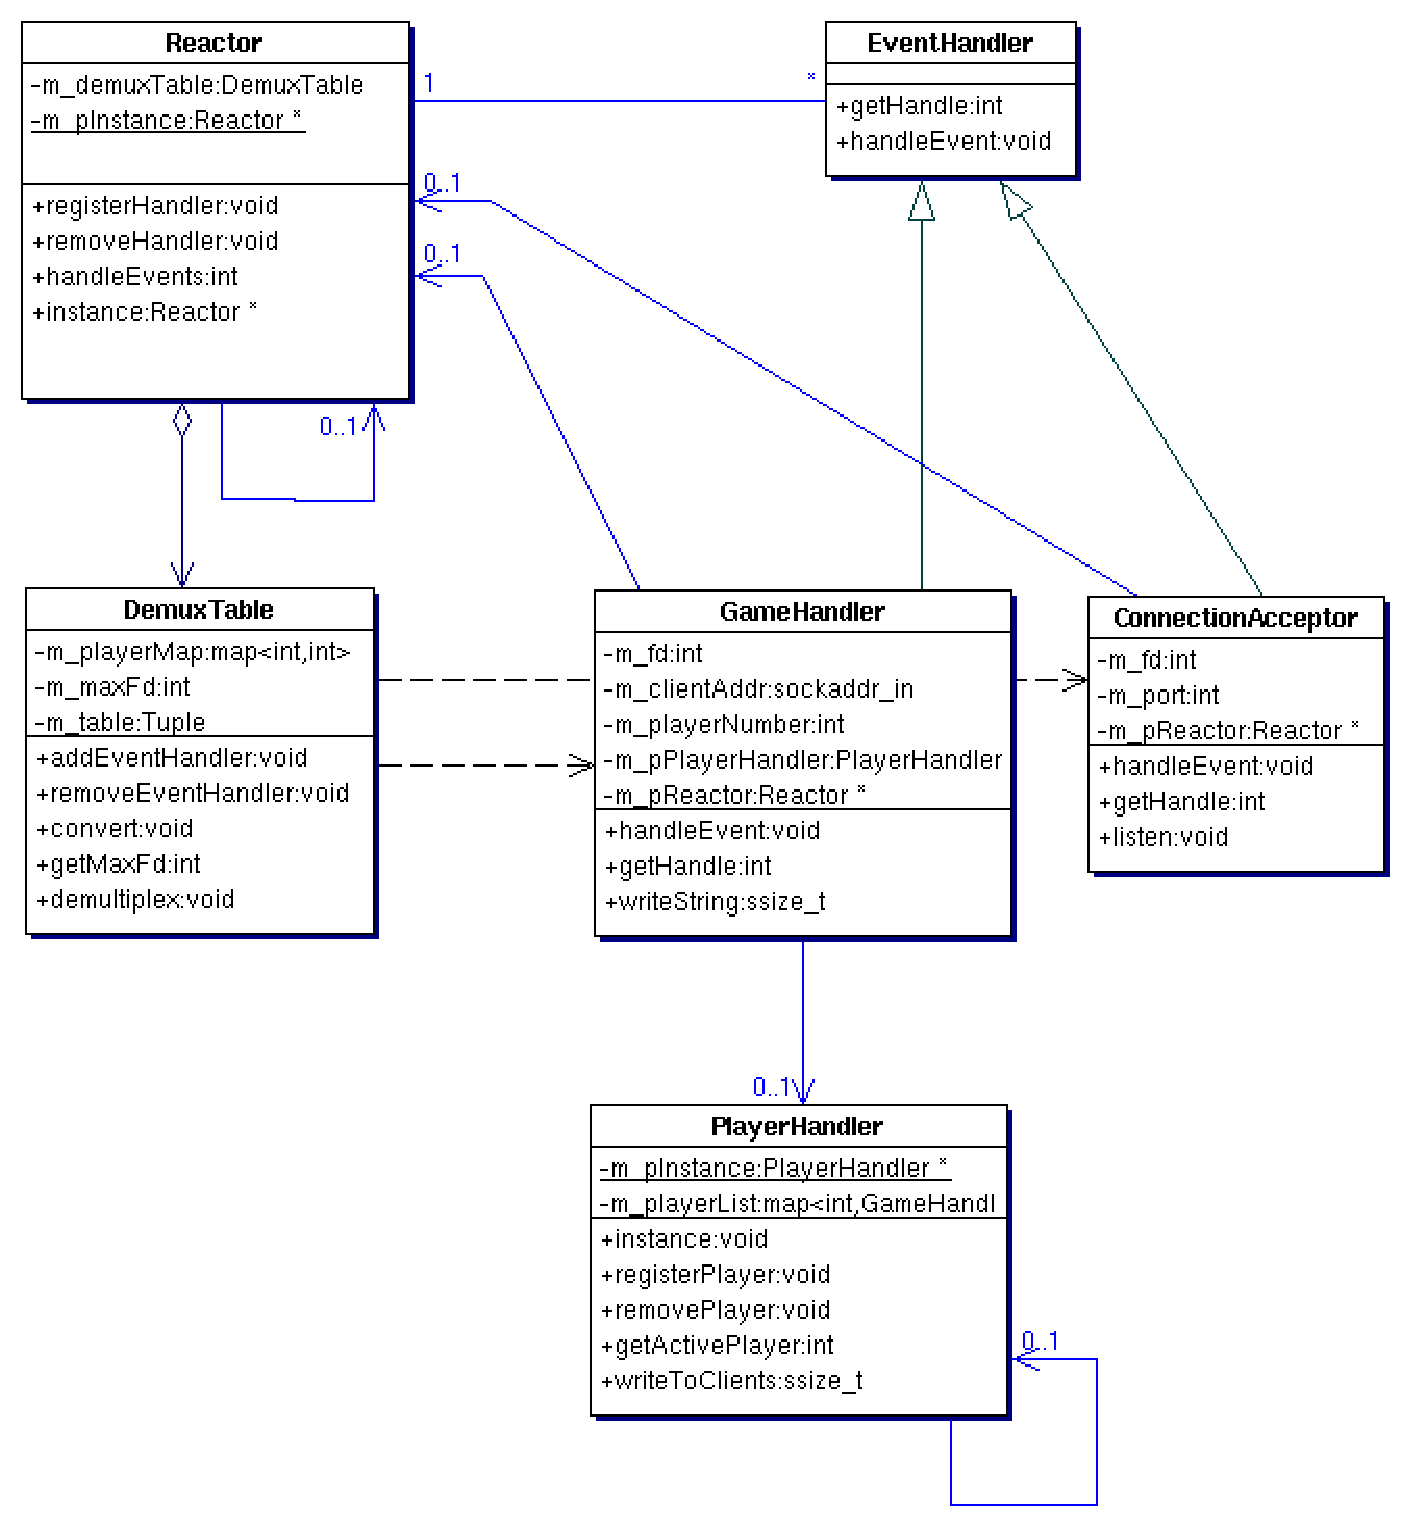
\includegraphics[width=12cm]{./images/reactor_klassendiagramm.pdf}}
  \end{center}
  \caption{Klassendiagramm Netzwerk/Server}
\end{figure}

\subsection{Beschreibung des Reactor Patterns}
Das Problem, dass sich bei einem Spiel, das erstens gewissen Geschwindigkeitsanforderungen gen"ugen muss und zweitens mehrere 
(mehr als 2) Mitspieler hat, ist, dass die Netzerwerkkommunikation speziell gel"ost werden muss, da alle Clients zu einem
nicht vorhersehbaren Zeitpunkt Meldungen zum Server schicken k"onnen. Da die Systemfunktionen, die f"ur die Kommunikation ben"otigt
werden (also read() und write() ) blockierend sind, muss entweder f"ur jeden Client ein seperater Prozess gestartet werden oder es 
muss ein geeignetes Pattern verwendet werden. Die erste L"osung w"are sehr einfach zu implementieren (wird auch sehr oft gemacht, zum
Beispiel bei Web Anwendungen), hat aber den Nachteil, dass bei einer Anwendung wie der unsrigen Interprozesskommunikation erforderlich
gewesen w"are, was sehr m"uhsam zu implementieren ist und auch Performance Nachteile mit sich bringt.
Die zweite L"osung mit dem Pattern erschien uns deshalb vorteilhafter, obwohl es auch nicht einfacher zu implementieren ist, 
aber die sinnvollere L"osung f"ur ein Spiel ist. 

Das Reactor Pattern hat folgende Vorteile
\begin{itemize}
	\item Wartezeiten und Antwortezeiten des Servers werden k"urzer da nicht blockierend auf einen Event eines einzigen Clients gewartet wird.
	\item Datendurchsatz wird erh"ort, da keine Daten zwischen einzelnen Prozessen ausgetauscht werden m"ussen.
	\item Sehr gute Wartungs- und Erweiterungseigenschaften, da "Anderungen nur an einem Ort gemacht werden m"ussen.
	\item Es ist kein Multithreading und keine Synchronisation im Server n"otig
\end{itemize}

Erreicht wird dies, indem synchron auf das Eintreffen von Ereignissen von verschiedenen Orten (Clients) gewartet wird. Diese Ereignisse
werden entgegengenommen, ausgewertet und an die bereitgestellten services weitergeleitet. Die Klassen und Methoden des Reactor 
Patterns werden in den folgenden Abschnitten erkl"art.
	
	
\subsection{Klasse Reactor (Singleton)}
Die Klasse ist daf"ur verantwortlich, die select() Funktion aufzurufen und anhand der Resultate, die sie von dieser Funktion erh"alt,
Reaktionen auszuf"uhren. Das heisst konkret, dass die select() Funktion, welche eine System Funktion ist, eine Meldung gibt, wenn ein 
Event eintrifft. Falls dies geschieht, ist die Reactor Klasse daf"ur verantwortlich, das richtige Handler Objekt (ConnectionAcceptor oder
GameHandler) aufzurufen. Damit stellt diese Klasse eine Abstraktion der select() Funktion dar und ist daf"ur verantwortlich, dass die
Handler Funktionen read() und connect() nur aufgerufen werden, wenn es tats"achlich n"otig ist. Damit wird gew"ahrleistet, dass
das System nicht blockiert, sondern dass alle Clients sehr schnell bedient und abgefragt werden k"onnen.
\subsubsection{Funktionen}
\begin{tabular}{p{50mm}p{90mm}}
	+registerHandler(EventHandler* pEventHandler, EventType eventType) : void  &  registriert einen neuen Event Handler (ConnectionAcceptor
	oder GameHandler) mit dem dazugeh"origen Event Typ in der Demultiplex Tabelle. \\
	+removeHandler(EventHandler* pEventHandler, EventType eventType)  : void  &  entfernt den Event Handler aus der Demultiplex Tabelle \\
	+handleEvents() : int     & f"uhrt die select() Funktion aus und ruft die 
	entsprechende Methode im ConnectionAcceptor bzw. im GameHandler auf. \\
	+instance() : Reactor* & gibt die Reactorinstanz zur"uck. \\ 
\end{tabular}


\subsection{Klasse EventHandler}
Diese Klasse ist eine rein virtuelle Klasse und stellt die Schnittstelle f"ur die abgeleiteten Klassen ConnectionAcceptor und GameHandler dar.

\subsection{Klasse ConnectionAcceptor}
Der ConnectionAcceptor ist daf"ur zust"andig, Verbindungsanfragen zu regeln. Das heisst, wenn sich ein Client mit dem Server verbinden m"ochte,
macht der ConnectionAcceptor eine neue Verbindung auf der Serverseite (erstellt einen neuen Filedeskriptor)
und falls es keine Fehler dabei gibt, wird ein neuer GameHandler erstellt.
\subsubsection{Funktionen}
\begin{tabular}{p{50mm}p{90mm}}
	+listen() : void & stellt einen Filedeskriptor mit der richtigen Struktur um Verbindungsanfragen entgegenzunehmen zur Verf"ugung und 
	registriert diesen beim Reactor. \\
	+handleEvent(int fd, EventType eventType) : void & ist eine "uberschriebene Funktion der Klasse EventHandler. Diese ist zust"andig, ankommende
	Anfragen f"ur eine Verbindung entgegenzunehmen und wenn kein Fehler auftritt, wird die Verbindung akzeptiert und ein neues GameHandler Objekt erstellt. \\
	+getHandle() : int & gibt den Filedeskriptor, der in der listen() Funktion bereitgestellt wurde zur"uck. \\
\end{tabular}

\subsection{Klasse GameHandler}
F"ur jeden Client, der sich verbunden hat, gibt es ein GameHandler Objekt. Dieses Objekt regelt die ganze Kommunikation zwischen Client und
Server f"ur diesen bestimmten Client. Das heisst, er nimmt alles, was vom Client zum Server geschickt wird entgegen und schreibt alles
vom Server zum Client. 
\subsubsection{Funktionen}
\begin{tabular}{p{50mm}p{90mm}}
	+handleEvent(int fd, EventType eventType) : void & ist eine "uberschriebene Funktion der Klasse EventHandler. Sie nimmt die
	Strings, die vom Client an den Server "ubermittelt wurden an und gibt diese an die PD weiter. \\
	+getHandle() : int & gibt den Filedeskriptor, der den GameHandler identifiziert zur"uck. \\
	+writeToClient(const char* str, size\_t n) : ssize\_t & Schreibt die Strings, die von der PD an die Clients "ubermittelt werden sollen zu dem
	Client, f"ur den das GameHandler Objekt zust"andig ist. \\
\end{tabular}

\subsection{Klasse DemuxTable}
Die Demultiplex Tabelle ist dazu da, die Filedeskriptoren mit ihren entsprechenden Eventtypen zu registrieren, 
damit bei einer Anfrage des Clients das richtige GameHandler Objekt
aufgerufen werden kann. Das heisst in dieser Tabelle sind alle File Deskriptoren mit den zugeh"origen Events gespeichert.
\subsubsection{Funktionen}
\begin{tabular}{p{50mm}p{90mm}}
	+convert(fd\_set\& read\_fds, fd\_set\& except\_fds) : void & konvertiert die Event-Typen um herauszufinden, was f"ur ein Event ansteht 
	(ein read oder connect Event)\\
	+addEventHandler(int fd, EventHandler* pEventHandler, EventType eventType) : void & ein EventHandler wird mit seinem Event Typ 
	in der Tabelle registriert.\\
	+removeEventHandler(int fd) : void & der EventHandler wird wieder aus der Tabelle entfernt.\\
	+getMaxFd() : int & der Zahlenwert des gr"ossten Filedeskriptors wird zur"uckgegeben.\\
	+demultiplex(int fdCount, fd\_set\& read\_fds, fd\_set\& except\_fds) : void & es wird anhand des Event-Typs in der Tabelle
	und des anstehenden Events herausgefunden, welche handleEvent() Funktion aufgerufen werden muss.\\
\end{tabular}

\section{Klasse PlayerHandler(Singleton)}
Im Netzwerk werden noch Assoziationen zwischen Filedeskriptor und Player (also Client) gemacht. Die PlayerHandler Klasse ist
von der Funktion her (nicht vom Aufbau) "ahnlich wie die Demultiplex Tabelle. Sie speichert f"ur jeden Client, also f"ur jeden GameHandler
einen Zeiger, damit sie diesen kennt. Wenn nun eine Meldung von der ServerPD an die Clients geschickt werden soll, wird in dieser Klasse
die entsprechende write() Funktion in allen GameHandler Objekten aufgerufen.
\subsubsection{Funktionen}
\begin{tabular}{p{50mm}p{90mm}}
	+registerPlayer(GameHandler* pGameHandler) : void & Wenn sich ein neuer Spieler angemeldet hat, wird hier das zugeh"orige GameHandler
	Objekt, das den Spieler identifiziert, registriert\\
	+removePlayer(GameHandler* pGameHandler) : void & Wenn die Verbindung zu einem Spieler nicht mehr besteht, wird der GameHandler dieses 
	Spielers hier entfernt.\\
	+getActivePlayer(GameHandler* pGameHandler) : int & gibt die Spielernummer (1-4) zur"uck. \\
	+instance() : WriteHandler* & die Instanz des PlayerHandler wird zur"uckgegeben. \\
\end{tabular}


\subsection{Client (Singleton)}
Die Client Klasse steuert die ganze Verbindung auf der Seite des Clients. Er macht die Verbindung zum Server, schickt daten an diesen und liest 
auch die Daten, die vom Server geschickt werden.
\subsubsection{Funktionen}
\begin{tabular}{p{50mm}p{90mm}}
	+makeConnection(const char* strPtr): int & er"offnet eine Verbindung zum Server mit der angegebenen IP\_Nummer und gibt den 
	Filedeskriptor, der diese Verbindung identifiziert zur"uck. \\
	+writeString(const char* str, size\_t n) : ssizt\_t & Schickt eine Meldung zum Server und gibt die L"ange der geschriebenen Zeichenkette
	zur"uck\\
	+readString() : ssize\_t & liest die Meldung vom Server und gibt die L"ange der Nachricht zur"uck. Die Funktion wird in einem
	eigenen Thread ausgef"uhrt, damit eine Meldung m"oglichst schnell entgegengenommen werden kann.\\
	+close() : void & schliesst die Verbindung zum Server \\
	+instance() : WriteHandler* & die Instanz des Clients wird zur"uckgegeben. \\
\end{tabular}


\section{Netzwerk Sequenzdiagramme}

\begin{figure}[H]
  \begin{center}
   \rotatebox{90}{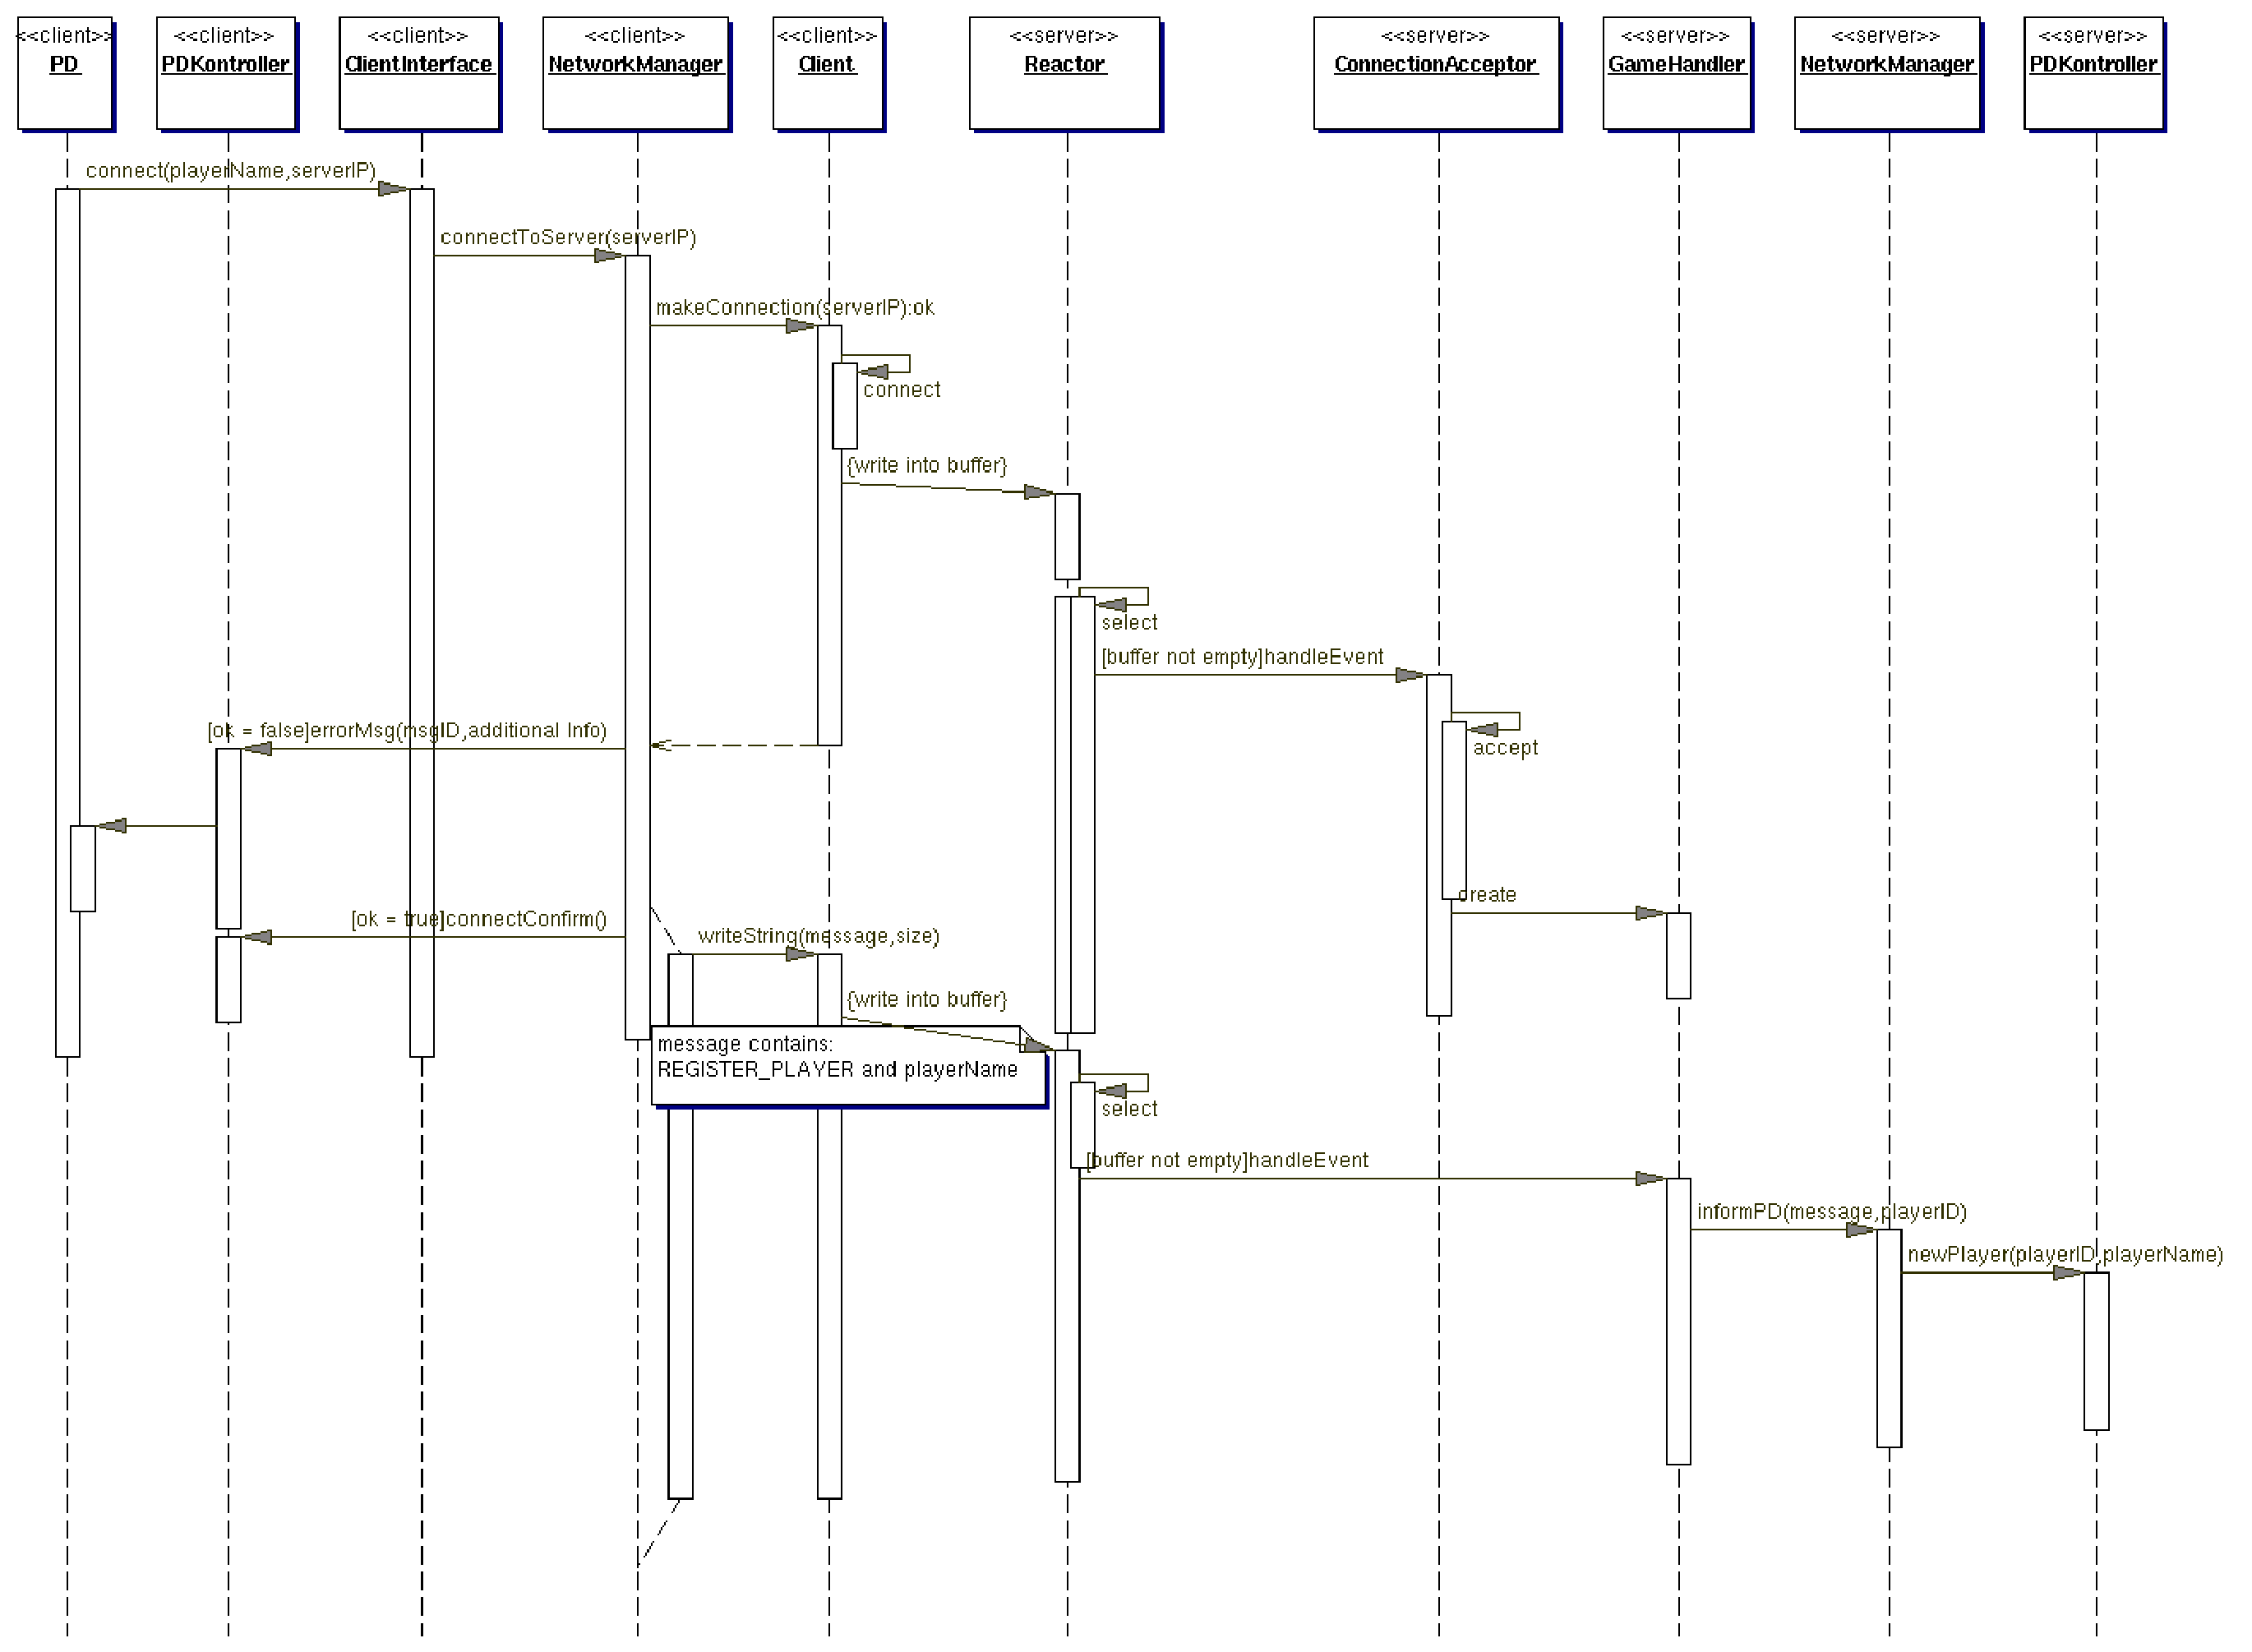
\includegraphics[width=18cm]{./images/clientconnect.pdf}}
  \end{center}
  \caption{Anmeldung des Clients bei einem Spiel}
\end{figure}

\begin{figure}[H]
  \begin{center}
    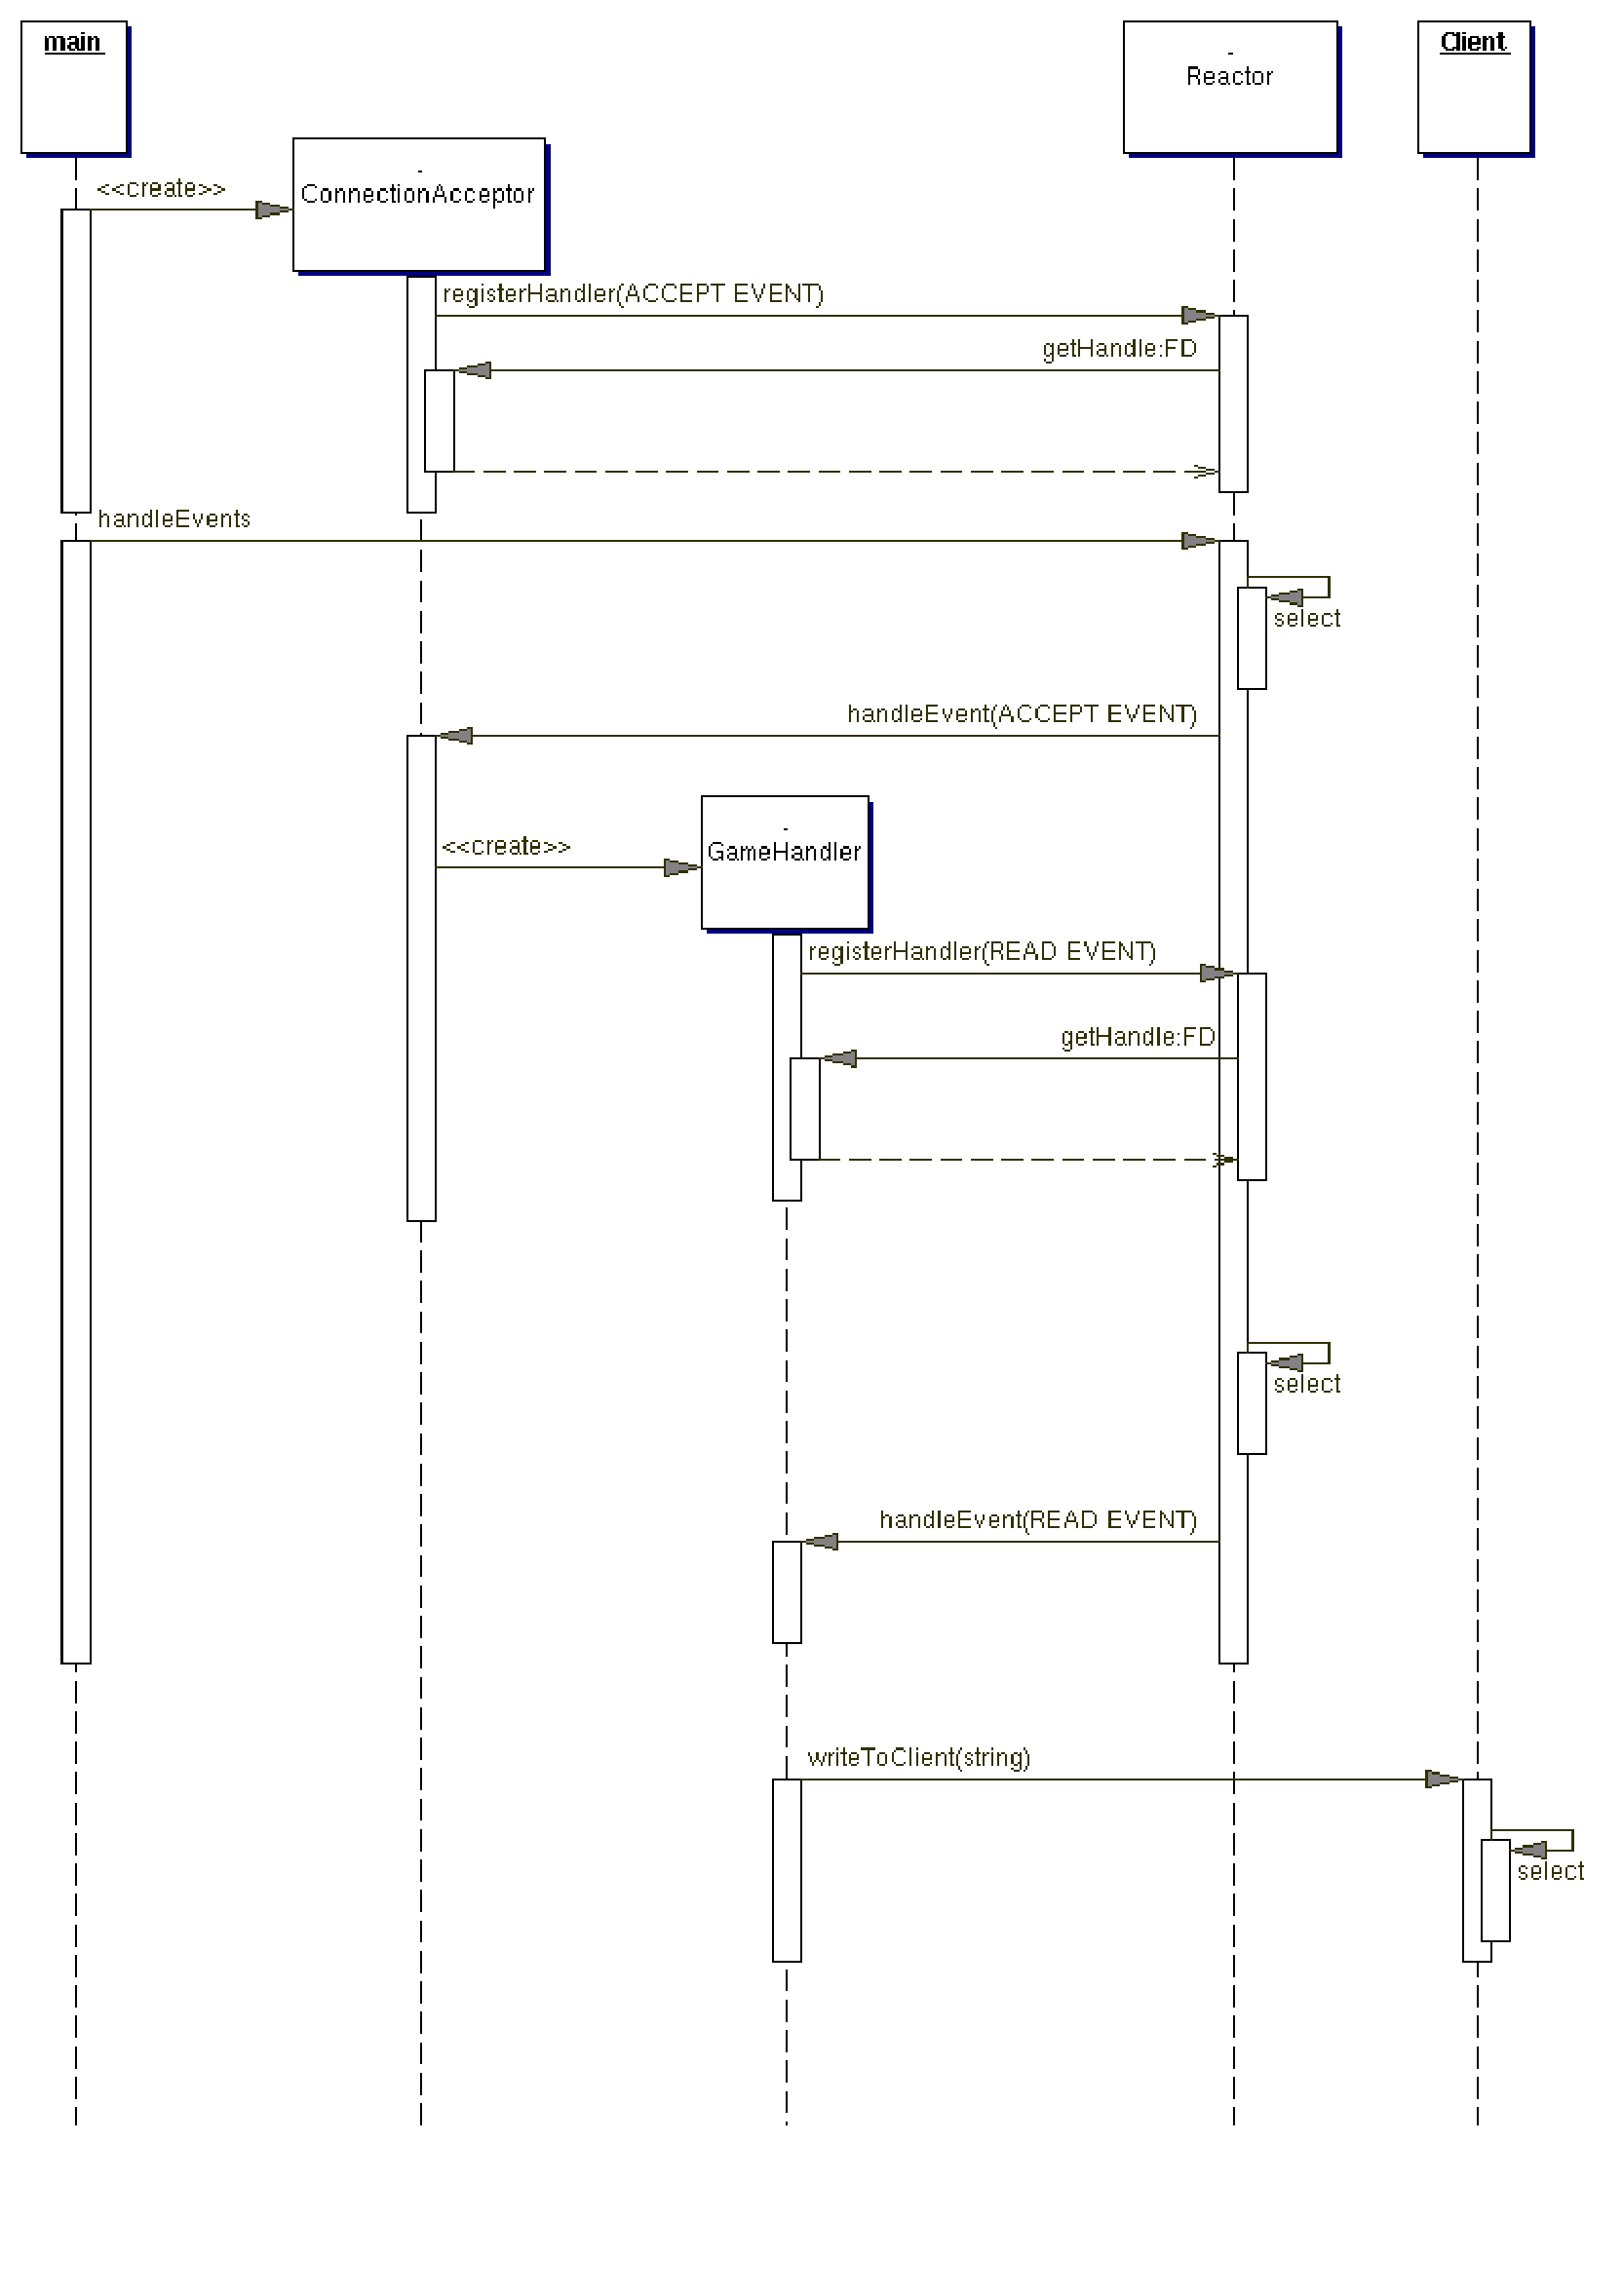
\includegraphics[width=12cm]{./images/sequenz_reactor.pdf}
  \end{center}
  \caption{Sequenzdiagramm Ablauf Server}
\end{figure}

\subsection{Erkl"arung Sequenzdiagramm Ablauf Server}
Im main Programm wird zuerst ein Objekt des ConnectionAcceptor erstellt. Dieser registriert sich anschliessend beim Reactor
und meldet damit, dass er f"ur ACCEPT EVENTS, das heisst f"ur ankommende Anfragen f"ur eine Verbindung, zust"andig ist.
Der Reactor registriert den ConnectionAcceptor in der Demultiplex Tabelle. Damit ist der erste Schritt gemacht und der Server
ist bereit, ankommende Verbindungsanfragen entgegenzunehmen.

Wenn das abgeschlossen ist, wird im Hauptprogramm (in einem eigenen Prozess) fortlaufend die Funktion handleEvents() des 
Reactors aufgerufen. Dieser f"uhrt den Systemaufruf select() durch, der pr"uft, ob eine Anfrage vorhanden ist. Ist dies der 
Fall, pr"uft er die Anfrage und im ersten Schritt wird das eine Verbindungsanfrage sein. Darauf ruft er handleEvent() im ConnectionAcceptor
auf, der die Anfrage entgegennimmt und bearbeitet. Falls es dabei keine Fehler gibt, wird ein neuer GameHandler erzeugt, der sich
gleich wieder beim Reactor registriert, diesmal aber f"ur READ EVENTS. Danach ist der Ablauf derselbe wie im ConnectionAcceptor.

Von nun an wird fortlaufend gepr"uft, ob eine Anfrage anliegt und wenn ja, wird der Typ der Anfrage ermittelt (READ oder ACCEPT Event) 
und die enstprechende Funktion im richtigen Objekt aufgerufen.

%end netzwerk design


%End Netzwerk Design

\chapter{Abschlusstest}
\begin{tabular}{p{30mm}p{70mm}}
Durchgef"uhrt am: &  11.7.2002 \\
Tester          : &  U. Heimann  \\

\end{tabular}
\linebreak

\section{Normaler Spielablauf}

\subsection{Spiel starten als Server}
\begin{tabular}{|p{50mm}|p{70mm}|p{20mm}|}
\hline
\textbf{Aktion} & \textbf{Erwartetes Ergebnis} & \textbf{Ergebnis}  \\
\hline
Programm von der Konsole aus Starten.  &
Programm startet, GUI wird angezeigt.  &
OK \\
\hline
Spielername im Dialog 'Spieleinstellungen' setzen, mit '"Ubernehmen' best"atigen.  &
Name wird "ubernommen (nicht sichtbar), Dialog verschwindet.  &
OK  \\
\hline
Netzwerkserver starten, 'Netzwerk $\rightarrow$  Spielserver starten...'  &
Dialog 'Server starten' erscheint.  &
OK  \\
\hline
Mit 'Starten' den Server starten.  &
Server wird gestartet (nicht sichtbar), der Spieler wird am eigenen Server mit dem eingegebenen Namen
  angemeldet. Es erscheint ein Dialog der die Verbindung best"atigt. Der eingegebene Name erscheint
  zuoberst in der Playerliste.  &
OK \\
\hline
Warten bis sich ein weiterer Spieler angemeldet hat.  &
Der Name des anderen Spielers erscheint in der Playerliste.  &
OK  \\
\hline
Mit 'Spiel $\rightarrow$ Neues Spiel..' das Spiel starten.  &
Spielumgebung wird erstellt. Spielfelddaten werden "ubermittelt. Das Spielfeld wird angezeigt.
  Wenn s"amtliche Spieler bereit sind wird das Spiel freigegeben.  &
OK  \\
\hline
\end{tabular}

\subsection{Spiel starten als Client}
\begin{tabular}{|p{50mm}|p{70mm}|p{20mm}|}
\hline
\textbf{Aktion} & \textbf{Erwartetes Ergebnis} & \textbf{Ergebnis}  \\
\hline
Programm von der Konsole aus Starten.  &
Programm startet, GUI wird angezeigt.  &
OK \\
\hline
Spielername im Dialog 'Spieleinstellungen' setzen, mit '"Ubernehmen' best"atigen.  &
Name wird "ubernommen (nicht sichtbar), Dialog verschwindet.  &
OK  \\
\hline
An einem Server anmelden, 'Netzwerk $\rightarrow$ Spielserver anmelden...'  &
Dialog 'Server anmelden' erscheint.  &
OK  \\
\hline
IP Adresse des Servers eingeben und mit 'Anmelden' best"atigen.  &
Der Spieler wird am Server mit dem eingegebenen Namen angemeldet. Es erscheint ein Dialog der die
  Verbindung best"atigt. Der eingegebene Name erscheint in der Playerliste.  &
OK \\
\hline
Warten bis sich weitere Spieler angemeldet haben.  &
Der Name der anderen Spieler erscheint in der Playerliste.  &
OK  \\
\hline
Warten bis der Server das Spiel startet.  &
Spielumgebung wird erstellt. Spielfelddaten werden "ubermittelt. Das Spielfeld wird angezeigt.
  Wenn s"amtliche Spieler bereit sind wird das Spiel freigegeben.  &
OK  \\
\hline
\end{tabular}

\subsection{Spielen}

\begin{tabular}{|p{50mm}|p{70mm}|p{20mm}|}
\hline
\textbf{Aktion} & \textbf{Erwartetes Ergebnis} & \textbf{Ergebnis}  \\

\hline
Mit den Pfeiltasten wird die Spielfigur auf den freien Feldern bewegt.  &
Die eigene Spielfigur bewegt sich gem"ass den Anweisungen.  &
OK  \\
\hline
Mit der Leertaste wird eine Bombe gelegt.  &
Auf dem Spielfeld an der Position der Spielfigur wird eine Bombe angezeigt. &
OK  \\
\hline
Die Bombe explodiert nach einer bestimmten Zeit von selbst.  &
Auf dem Spielfeld wird der Feuerstrahl angezeigt. W"ande die vom Feuerstrahl getroffen werden, werden
  gel"oscht. Der Feuerstrahl verschwindet von selbst wieder.  &
OK  \\
\hline
Mehrere Bomben werden zeitlich versetzt nebeneinander gelegt.  &
Die Explosion der ersten Bombe l"ost die anderen Bomben ebenfalls aus.  &
OK  \\
\hline
Der andere Spieler bewegt seine Spielfigur und legt Bomben.  &
Die Spielfigur des Gegners bewegt sich auf dem Spielfeld gem"ass den Anweisungen des Gegners auf dem anderen
  Computer. Bomben werden angezeigt und explodieren. &
OK  \\
\hline
Eine Spielfigur wird von einem Feuerstrahl getroffen.  &
Die getroffene Spielfigur wird vom Spielfeld entfernt. Wenn nur noch ein Spieler auf dem Feld ist, erscheint
  eine Meldung mit dem Namen des Siegers. Das Spiel wird beendet. &
OK  \\
\hline
Der Server startet mit 'Spiel $\rightarrow$ Neues Spiel..' ein neues Spiel.  &
Ein neues Spielfeld wird angezeiget. Alle Spieler sind wieder dabei und k"onnen mitspielen.  &
OK  \\
\hline
\end{tabular}


\subsection{Spiel beenden}

\begin{tabular}{|p{50mm}|p{70mm}|p{20mm}|}
\hline
\textbf{Aktion} & \textbf{Erwartetes Ergebnis} & \textbf{Ergebnis}  \\
\hline
Ein Spieler (nicht der Server) schliesst seine Anwendung.  &
Der Spieler wird beim Server abgemeldet und das Programm wird geschlossen. Die verbliebenen Spieler
  erhalten eine Meldung, dass sich der Spieler abgemeldet hat. Der Name des Spielers verschwindet aus
  der Playerliste.  &
OK  \\
\hline
Der Spieler mit dem Server schliesst seine Anwendung.  &
Der Server meldet sich bei allen Clients ab und das Programm wird geschlossen. Die verbliebenen Spieler
  erhalten eine Meldung, dass sich der Server abgemeldet hat. S"amtliche Namen der Spieler verschwinden
  aus der Playerlist.  &
OK  \\
\hline
\end{tabular}


\section{Varianten Spielablauf}

\subsection{Spiel starten}

\begin{tabular}{|p{50mm}|p{70mm}|p{20mm}|}
\hline
\textbf{Aktion} & \textbf{Erwartetes Ergebnis} & \textbf{Ergebnis}  \\
\hline
Spiel vom Konqueror aus starten.  &
Spiel startet, GUI wird angezeigt.  &
FAILED   \\
 & & Das Spiel wird gestartet, die Grafiken f"ur das Spielfeld werden jedoch nicht gefunden. \\
\hline
Ein neuer Spieler versucht sich w"ahrend eines laufenden Spiels eine Verbindung aufzubauen.  &
Der Spieler kann die Verbindung aufbauen, kann aber keinen Einfluss auf das laufende Spiel nehmen.
  Beim n"achsten Spielstart spielt der Spieler auch mit.  &
OK  \\
\hline
Ein Spieler gibt vor dem Anmelden am Server keinen Spielernamen ein.  &
Er erscheint in der Playerliste als 'anonymous'.  &
OK  \\
\hline

\end{tabular}


\section{Fehlerf"alle}

\begin{tabular}{|p{50mm}|p{70mm}|p{20mm}|}
\hline
\textbf{Aktion} & \textbf{Erwartetes Ergebnis} & \textbf{Ergebnis}  \\
\hline
Der Spieler gibt beim Verbinden mit einem Server eine ung"ultige IP ein. &
Es wird eine Meldung ausgegeben, dass mit dem Server keine Verbindung aufgebaut werden konnte.  &
OK  \\
\hline
Mitten im Spiel schliesst ein Spieler (nicht der Server) seine Anwendung.  &
Die Figur des Spielers wird zerst"ort und verschwindet vom Spielfeld. Der Name des Spielers wird aus der
  Playerliste entfernt. Das Spiel l"auft weiter.  &
OK \\
\hline
Mitten im Spiel schliesst der Server seine Anwendung.  &
Das Spiel wird beendet. Die verbliebenen Spieler erhalten eine Meldung, und s"amtliche Namen werden aus
  der Playerliste gel"oscht.  &
OK \\
\hline
\end{tabular}


\chapter{Buglist}


\begin{tabular}{|p{5mm}|p{60mm}|p{65mm}|p{10mm}|}
\hline
\textbf{Nr.} & \textbf{Fehlerbild} & \textbf{M"ogliche Ursache} & \textbf{Status}  \\
\hline
1 &
Spielfiguren werden erst angezeigt wenn sie bewegt werden.  &
Positionen der Figuren werden beim Spielfeldaufbau nicht "ubermittelt.  &
FIXED  \\
\hline
2 &
Wenn ein Spieler die Verbindung abbricht wird der Name in der Playerliste nicht gel"oscht.  &
Im GUI wird auf das 'removePlayer' Ereigniss nicht reagiert.  &
FIXED  \\
\hline
3 &
Wenn das Programm beendet wird muss ca. 30 - 60 Sekunden gewartet werden bis wieder ein Server gestartet
  werden kann.  &
Eventuell wird der verwendete Socket vom System nicht unmittelbar freigegeben.  &
 \\
\hline
4 &
Wenn das Spiel vom Konqueror aus gestartet wird, wird das Spielfeld nicht angezeigt.
  Das Spiel funktioniert sonst normal.  &
Die Grafiken der W"ande, Mauern, etc. k"onnen nicht geladen werde. Eventuell falscher Arbeitspfad.  &
 \\
\hline


\end{tabular}


%\end{document}

\chapter{Installation und Bedienung}
	\section{Installation}	
		Die Installation erfolt wie bei den meisten Programmen unter Linux. Zuerst muss das tar Archiv (falls nicht schon entpackt)
		mit dem Befehl
		\begin{verbatim}
			tar -xvzf <name>.tgz
		\end{verbatim}
		entpackt werden. Anschliessend wechseln Sie in das neu erstellte Verzeichnis und kompilieren und installieren das Programm.
		Das geschieht mit den folgenden Befehlen
		\begin{verbatim}
			cd netbomber
			make
			make install
		\end{verbatim}

		Eine Ausf"uhrlichere Beschreibung finden sie in der mitgelieferten README Datei.

	\section{Bedienungsanleitung}
		Das Spiel \textsc{NetBomb} k"onnen Sie mit dem von der Konsole aus starten. Dazu wechseln Sie zuerst in das Verzeichnis,
		in das sie \textsc{NetBomb} installiert haben. Anschliessen geben Sie die Befehle
		\begin{verbatim}
			cd netbomber
			./netbomber
		\end{verbatim}
		ein. Damit wird das Programm gestartet. Es erscheint ein Fenster mit dem Spiel. 

		Als erstes k"onnen Sie unter dem Menu \textit{Optionen $\rightarrow$} Tastaturbelegung Ihren Namen eingeben.
		"Ubernehmen Sie Ihre Eingabe mit der Taste \textit{"Ubernehmen} und Beenden Sie den Dialog mit \textit{Abbrechen}.
		Anschliessend haben Sie zwei M"oglichkeiten. Sie k"onnen 
		\begin{enumerate}
			\item Einen Server starten, bei dem sich ihre Mitspieler anmelden k"onnen. Dazu gehen Sie folgendermassen vor
			\begin{enumerate}
				\item W"ahlen Sie  \textit{Netzwerk $\rightarrow$ Spielserver starten} und w"ahlen Sie dann die Anzahl Mitspieler.
							Anschliessen k"onnen Sie mit der Taste \textit{Starten} den Server starten.
				\item Es erscheint eine Meldung die Ihnen Mitteilt, ob sie erfolgreich eine Spielserver starten konnten. Best"atigen
							sie diesen Dialog. Danach erscheint in der Spielerliste (Liste rechts oben) ihr Name.
				\item Wenn Sie erfolgreich einen Server gestartet haben, m"ussen Sie warten, bis sich Ihre Mitspieler auf Ihren 
							Server eingeloggt haben. Sie sehen die Spieler, die Spielbereit sind in der Spielerliste.
				\item Sobald gen"ugend Spieler angemeldet sind, k"onnen sie mit \textit{Spiel $\rightarrow$ Neues Spiel} ein neues 
							Spiel starten.
				\item Have fun!
			\end{enumerate}
			\item Sich bei einem Server anmelden, um mitzuspielen. Dazu gehen Sie folgendermassen vor
			\begin{enumerate}
				\item Sie k"onnen sich mit \textit{Netzwerk $\rightarrow$ Spielserver anmelden} bei einem Server anmelden.
				\item	Es erscheint ein Fenster, in den Sie die IP - Adresse des Servers eingeben m"ussen. Tun Sie das und
							best"atigen Sie die Eingabe mit \textit{Anmelden} oder brechen Sie die Eingabe \textit{Abbrechen} ab.
				\item Sobald der Spieler, der den Server gestartet hat, beginnt das Spiel
				\item Have fun!
			\end{enumerate}
		\end{enumerate}

		
		\noindent
		Sie k"onnen das Spiel jederzeit mit \textit{Spiel $\rightarrow$ Beenden} schliessen. \\

		\noindent
		Viel Spass beim Spielen.
		Das \textsc{NetBomb} - Team


\begin{appendix}
\chapter{Glossar}
\label{glossar}

\section{Namen}

\begin{tabular}{ll}

STEK & Stefan K"unzle \\
REH  & Ren\'e Herrmann \\
MIE  & Michael Egli \\
UHEI & Urs Heimann \\

\end{tabular}

\section{Spielbegriffe}

\begin{tabular}{p{30mm}p{110mm}}

  Spielfeld      & Besteht aus freien Feldern, Mauern und W"anden. Der Spieler kann seine Figur auf den freien Feldern bewegen. \\
  Freies Feld    & Darauf kann sich die Spielfigur frei bewegen und Bomben legen. Es k"onnen sich Powerups darauf befinden. \\
  Mauer          & Ein dauerhaftes Hinderniss auf dem Spielfeld. Sie kann nicht durch eine Bombe zerst"ort werden und bleibt
                   w"ahrend dem ganzen Spiel unver�ndert. \\
  Wand           & Ein Hindernis auf dem Spielfeld das durch eine Bombe zerst"ort werden kann. Sie wird dann zu einem freiem Feld.
                   Sie kann ein Powerup enthalten das nach der Sprengung auf dem Feld liegenbleibt. \\
  Spielfigur     & Wird vom Spieler auf den freien Feldern bewegt und kann Bomben legen. Sie kann nicht durch Mauern oder W"ande gehen.
                   Tritt sie auf ein Feld mit einem Powerup nimmt sie dieses auf. Wird sie von einem Feuerstrahl getroffen,
                   stirbt sie und verschwindet vom Spielfeld. \\
  Bombe          & Wird von der Spielfigur auf das Spielfeld gelegt und explodiert nach einer bestimmten Zeit.
                   Beim explodieren erzeugt sie f"ur jede Himmelsrichtung einen Feuerstrahl.\\
  Feuerstrahl    & Auswirkung der explodierenden Bombe. Er ist ein oder mehrere Felder lang und zerst"ort W"ande, Spielfiguren und Powerups.
                   Seine L"ange h"angt davon ab von welcher Spielfigur die Bombe gelegt wurde und wieviele Flamme-Powerups diese aufgenommen hat. \\
  Serie          & Mehrere hintereinander gelegte Bomben bevor die erste explodiert. (zu beginn nur eine Bombe in Serie m"oglich) \\
  Bombe-Powerup  & Liegt auf einem freien Feld und kann von der Spielfigur aufgenommen werden.
                   Es erm"oglicht ihr eine Bombe mehr in Serie zu legen. \\
  Flamme-Powerup & Kann von der Spielfigur aufgenommen werden und erh"oht die Reichweite seiner Bomben um ein Feld. \\
  Spielelement   & Sammelbegriff f"ur Mauer, Wand, Bombe, Powerups. \\
  Ojekt des Spielfeldes & Spielelemente, Spielfigur\\

\end{tabular}

\section{Technische Begriffe}

\begin{tabular}{p{30mm}p{110mm}}

  GUI & Grafisches User Interface. "Uber dieses interagiert der Benutzer, in unserem Fall der Spieler. \\

\end{tabular}


\chapter{"Anderungsgeschichte}


\begin{tabular}{|p{15mm}|p{15mm}|p{15mm}|p{15mm}|p{55mm}|}
  \hline \textbf{Datum} & \textbf{Wer} & \textbf{Version} & \textbf{Kapitel} & \textbf{"Anderung} \\
  \hline 06.04.02 & alle & 0.1 & 1-3 & Erstellung Kapitel 1-3 (MS 1) \\
  \hline 06.04.02 & REH,MIE & 0.1.1 & 1-3 & "Uberarbeiten V 0.1 \\
  \hline 12.04.02 & alle & 0.2 & 4 & Erstellung Kapitel 4 (MS 2) \\
  \hline 19.04.02 & alle & 0.2.1 & 4,5 & Vervollst�ndigt und korrigiert \\
  \hline 26.04.02 & alle & 0.3 & 5,6 & Kap 5 "uberarbeitet und Kap. 6 neu erstellt \\
  \hline 07.05.02 & STEK,UHEI & 0.4 & 6 & GUI und PD Design eingef"ugt \\
  \hline 12.06.02 & alle & 1.0 & alles & "uberarbeiten und vervollst"andigen zur Abgabe \\
	\hline
\end{tabular}

\end{appendix}

\end{document}
